% Allways use memoir class, 
\documentclass[a4paper,
final,
book,english]{memoir}

% inputenc tells latex that the encoding is utf8
\usepackage[utf8]{inputenc}

% babel knows how the language works, word division, and so on. (the language is set in the \documentclass option)
\usepackage{babel}

% Helps with the fonts
\usepackage[T1]{fontenc}

% for making better word division, and think it should only be used in danish. uncomment if you use danish.
%\renewcommand{\danishhyphenmins}{22}

%if you  \emph{} something that is already in italy it becomed bold and italy
%\usepackage{fixltx2e}
\renewcommand*\eminnershape{\bfseries \itshape}

%For using math in latex
\usepackage{amsmath}
\usepackage{amssymb}
\usepackage{amsthm}

%For link in document hidelinks removes the ugly red color
\usepackage[hidelinks]{hyperref}
%Make the read around the url go away

\usepackage{alltt}

\usepackage[colorinlistoftodos,obeyFinal]{todonotes}

\newtheorem{mydef}{Definition}
\newtheorem{theorem}[mydef]{Theorem}
\newtheorem{Lemma}[mydef]{Lemma}
\newtheorem{Corollary}[mydef]{Corollary}

%\numberwithin{mydef}{chapter}
%\numberwithin{theorem}{chapter}
%\numberwithin{Lemma}{chapter}

\usepackage{graphicx,wrapfig,lipsum}

\usepackage{algorithm}
\usepackage{caption}
\usepackage{subcaption}

\usepackage[noend]{algpseudocode}
\algnewcommand\algorithmicforeach{\textbf{for each}}
\algdef{S}[FOR]{ForEach}[1]{\algorithmicforeach\ #1\ \algorithmicdo}


\settocdepth{subsection}
\setsecnumdepth{subsection}
\usepackage{alltt}
\usepackage{makeidx}
\makeindex

%  \newlength\myindent
%  \setlength\myindent{2em}
%  \newcommand\bindent{
%    \begingroup
%    \setlength{\itemindent}{\myindent}
%    \addtolength{\algorithmicindent}{\myindent}
%  }
%  \newcommand\eindent{\endgroup}

\usepackage{tikz}
\usetikzlibrary{positioning}
\usepackage{pgf}
\usepackage{mathrsfs}
\usetikzlibrary{arrows}
\usepackage{tablefootnote}
\newcommand*{\addheight}[2][.5ex]{%
  \raisebox{0pt}[\dimexpr\height+(#1)\relax]{#2}%
}
\usepackage{pgfplots} 

\makeatletter
\newcommand{\multiline}[1]{%
  \begin{tabularx}{\dimexpr\linewidth-\ALG@thistlm}[t]{@{}X@{}}
    #1
  \end{tabularx}
}
\makeatother

\algnewcommand{\LeftComment}[1]{\Statex \(\triangleright\) #1}



\newcommand{\gerth}[1]{\todo[color=black!40]{#1}}
\newcommand{\nick}[1]{\todo[color=green!40]{#1}}
\newcommand{\peter}[1]{\todo[color=blue!40]{#1}}

%----------------------------------------------------------------------------------------
%	TITLE SECTION
%----------------------------------------------------------------------------------------

\newcommand{\horrule}[1]{\rule{\linewidth}{#1}} % Create horizontal rule command with 1 argument of height

\pretitle{%
  \begin{center}
  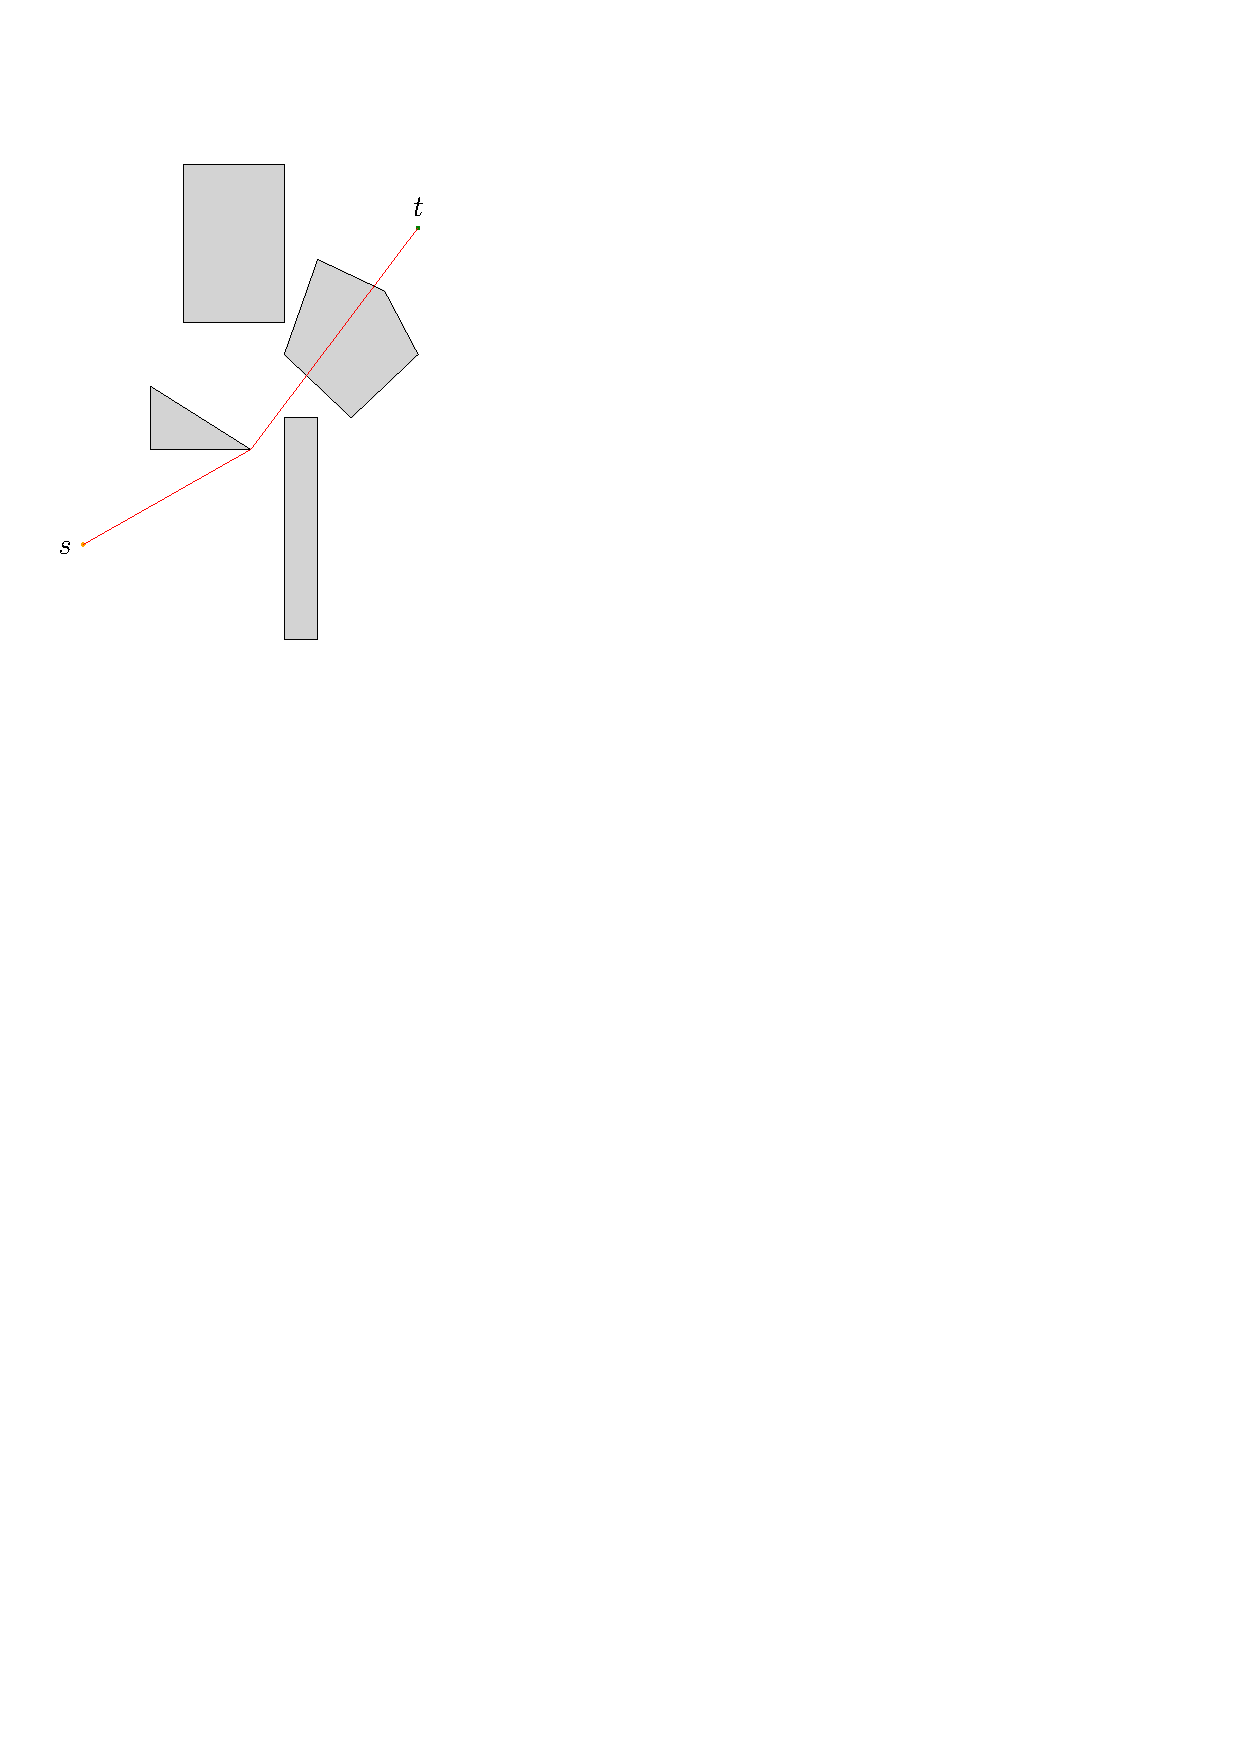
\includegraphics[width=6cm]{figures/frontpage.pdf}
}

\posttitle{
	\end{center}
}
\title{
	\\
	\normalfont \normalsize 
    \vspace{2cm}
	\textsc{Aarhus University, Department of Computer Science} \\ [25pt] % Your university, school and/or department name(s)
	\horrule{0.5pt} \\[0.4cm] % Thin top horizontal rule
    \huge Master's Thesis \\
    \huge Shortest Path Problem in the Plane with Polygonal Obstacle Violations 
	\horrule{2pt} \\[0.5cm] % Thick bottom horizontal rule 
}

\author{
	Nick Bakkegaard - 20114270\\
	Peter Burgaard - 201209175\\
	{\small Advisor: Gerth Stølting Brodal}
} % Your name

\date{\normalsize\today} % Today's date or a custom date

\begin{document}

\frontmatter

\maketitle % Print the title

\thispagestyle{empty}

\newpage

\chapter*{Abstract}

This thesis is dedicated to exploring a solution to the shortest path in the
plane with polygonal obstacles violation problem. First, we explore and
implement a naive $O(n^3)$ solution to introduce the problem and key concepts.
Next, we move on to a $O(n \log n)$ algorithm which solves the shortest path in
the plane without polygonal obstacle problem, which is due to Hershberger and
Suri \cite{HershbergerS99}, where one build a shortest path map, in which one
can find the shortest path without violations in time $O(\log n)$. This
algorithm is extended to the main $O(k^2 n \log n)$ solution which is due to
Hershberger, Kumar and Suri \cite{HershbergerKS17}, in which the algorithm
builds a shortest $k$-path map, from which the shortest path with $k$
violations can be queried in $O(\log n)$ time. 

\newpage
\chapter*{Acknowledgement}

We want to thank Niels Bross and Kresten Maigaard Axelsen for being great office buddies and also being up for a nice chat and a cup of coffee. 

We also want to thank Andrease Malling Østergaard and Andreas Østergaard Nielsen for being great skribbl.io opponents. 
\newpage


\tableofcontents
\listoffigures
\listofalgorithms
\listoftables
\mainmatter

\chapter{Introduction} 
Given a starting point $s$, an endpoint $t$ and a set of
polygons $\mathcal{O}$ in the plane, we want to find the shortest path from $s$ to $t$ 
without traveling through the interior of any polygon in $\mathcal{O}$. 
This is an old and well studied problem, and historically there have been two
conceptually different approaches to the problem, one using visibility graphs and
another using the continuous Dijkstra method. 

The visibility graph approach is to construct a graph of all paths between every pair 
of vertices in the plane which doesn't go through an interior of an obstacle. 
These paths are called legal paths. Then the shortest path is found by then running a 
single source shortest path algorithm on that graph. A problem of this approach
is the complexity of the graph can be $\Theta(n^2)$, with $n$ begin the number of vertices of the polygons,
which makes it difficult to get below this threshold. 

The continuous Dijkstra method works by simulating a \emph{wavefront propagation}.
A wavefront is a circular arch which originates from a point and expands in at unit-speed
(non-changing speed) such that all points of the boundary of the arch have equal distance 
$d$ to the generator point from which the wavefront originated, at every time $t$. 
This point is the source (start point) $s$, see figure \ref{fig:simplewavefront}.

\begin{figure}[H]
    \centering
	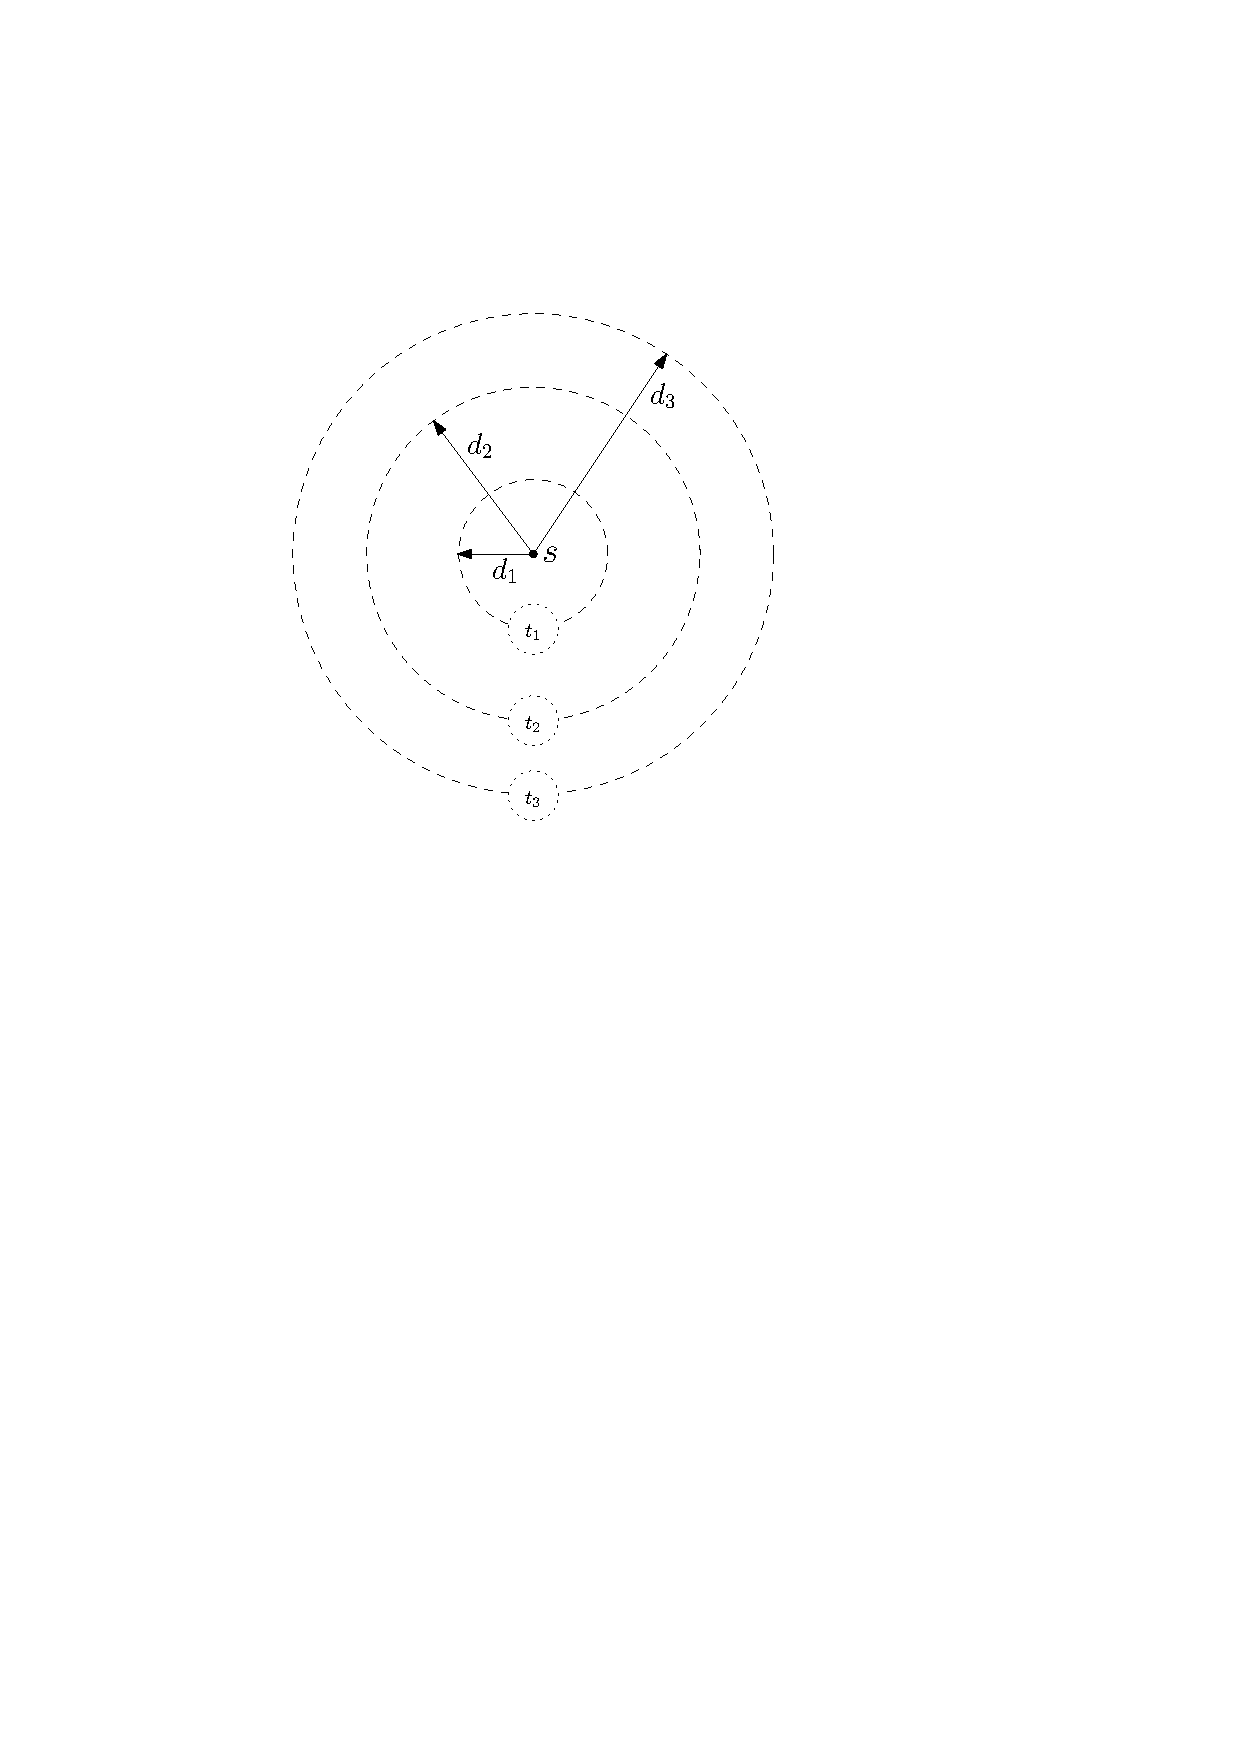
\includegraphics[width=0.5\textwidth]{figures/simplewavefront.pdf}
	\caption{A right turn formed by three points}
    \label{fig:simplewavefront}
\end{figure}

From the figure we can see that since the wavefront expands at unit-speed, the time distance
$d_i$ at time $t_i$ are equal, are one therefore is only concerned with the time $t$.
Every time a vertex $v$ is reached a new wavefront starts emitting from $v$. This way
the plane will be divided into different areas depending on which wavefront encapsulates it,
see figure \ref{fig:introductiontowavefront}.

\begin{figure}[H]
    \centering
	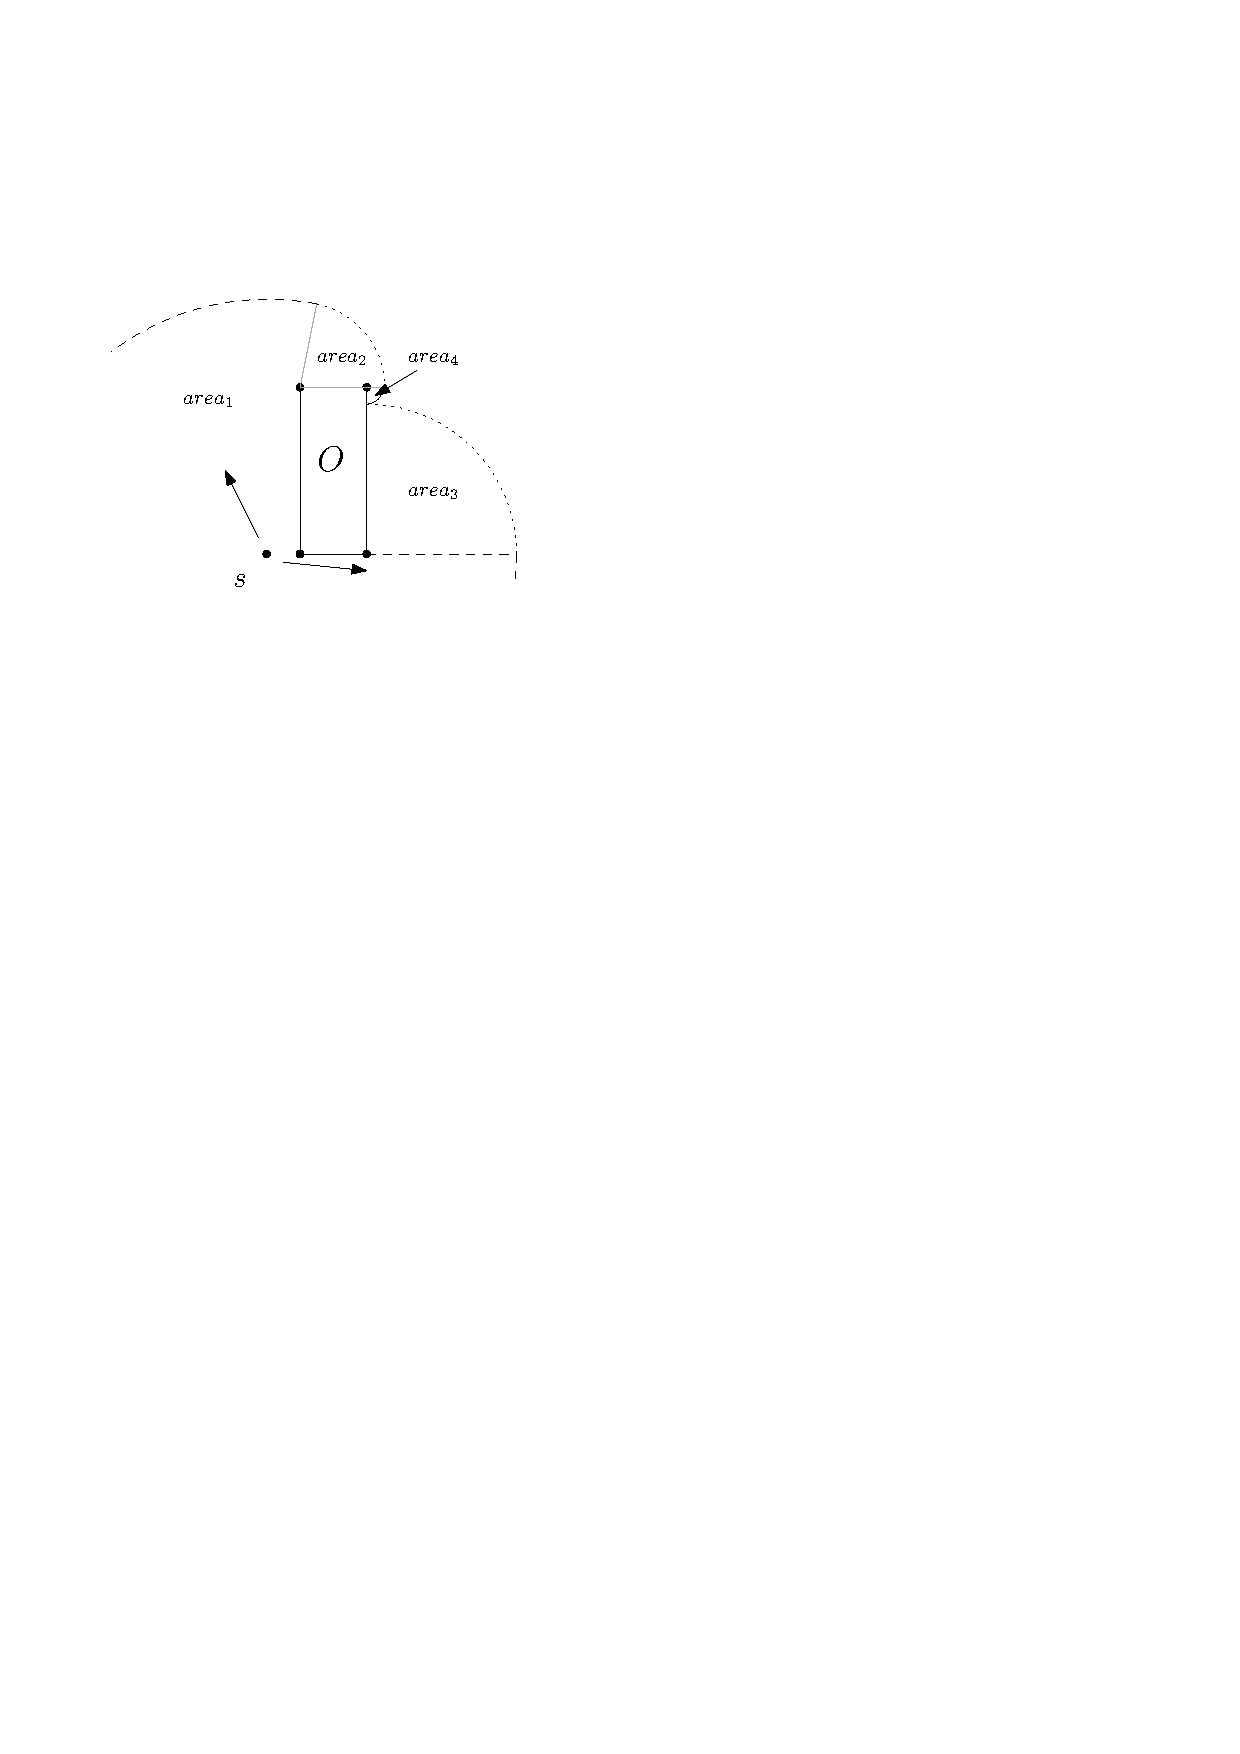
\includegraphics[width=0.5\textwidth]{figures/introductiontowavefront.pdf}
	\caption{A simple example of the wavefront spreading in the plane around an obstacle $O$
	         an encapsulating different areas.}
     \label{fig:introductiontowavefront}
\end{figure}

In 1999 Hershberger and Suri published the paper "an optimal algorithm for euclidean shortest 
paths in the plane"\cite{HershbergerS99} in which they presented an optimal $O(n\log n)$ time 
algorithm which matched the lower bound of the problem (see Chapter \ref{chapter:lowerbound}), 
using an implementation of the continuous Dijkstra method.

In 2017 they, together with Kumar, looked at a generalization of the problem:
given the same setting as before, one is now allowed to go through up to $k$ obstacles.
See figure \ref{fig:shortestkpath}.

\begin{figure}[H]
    \centering
	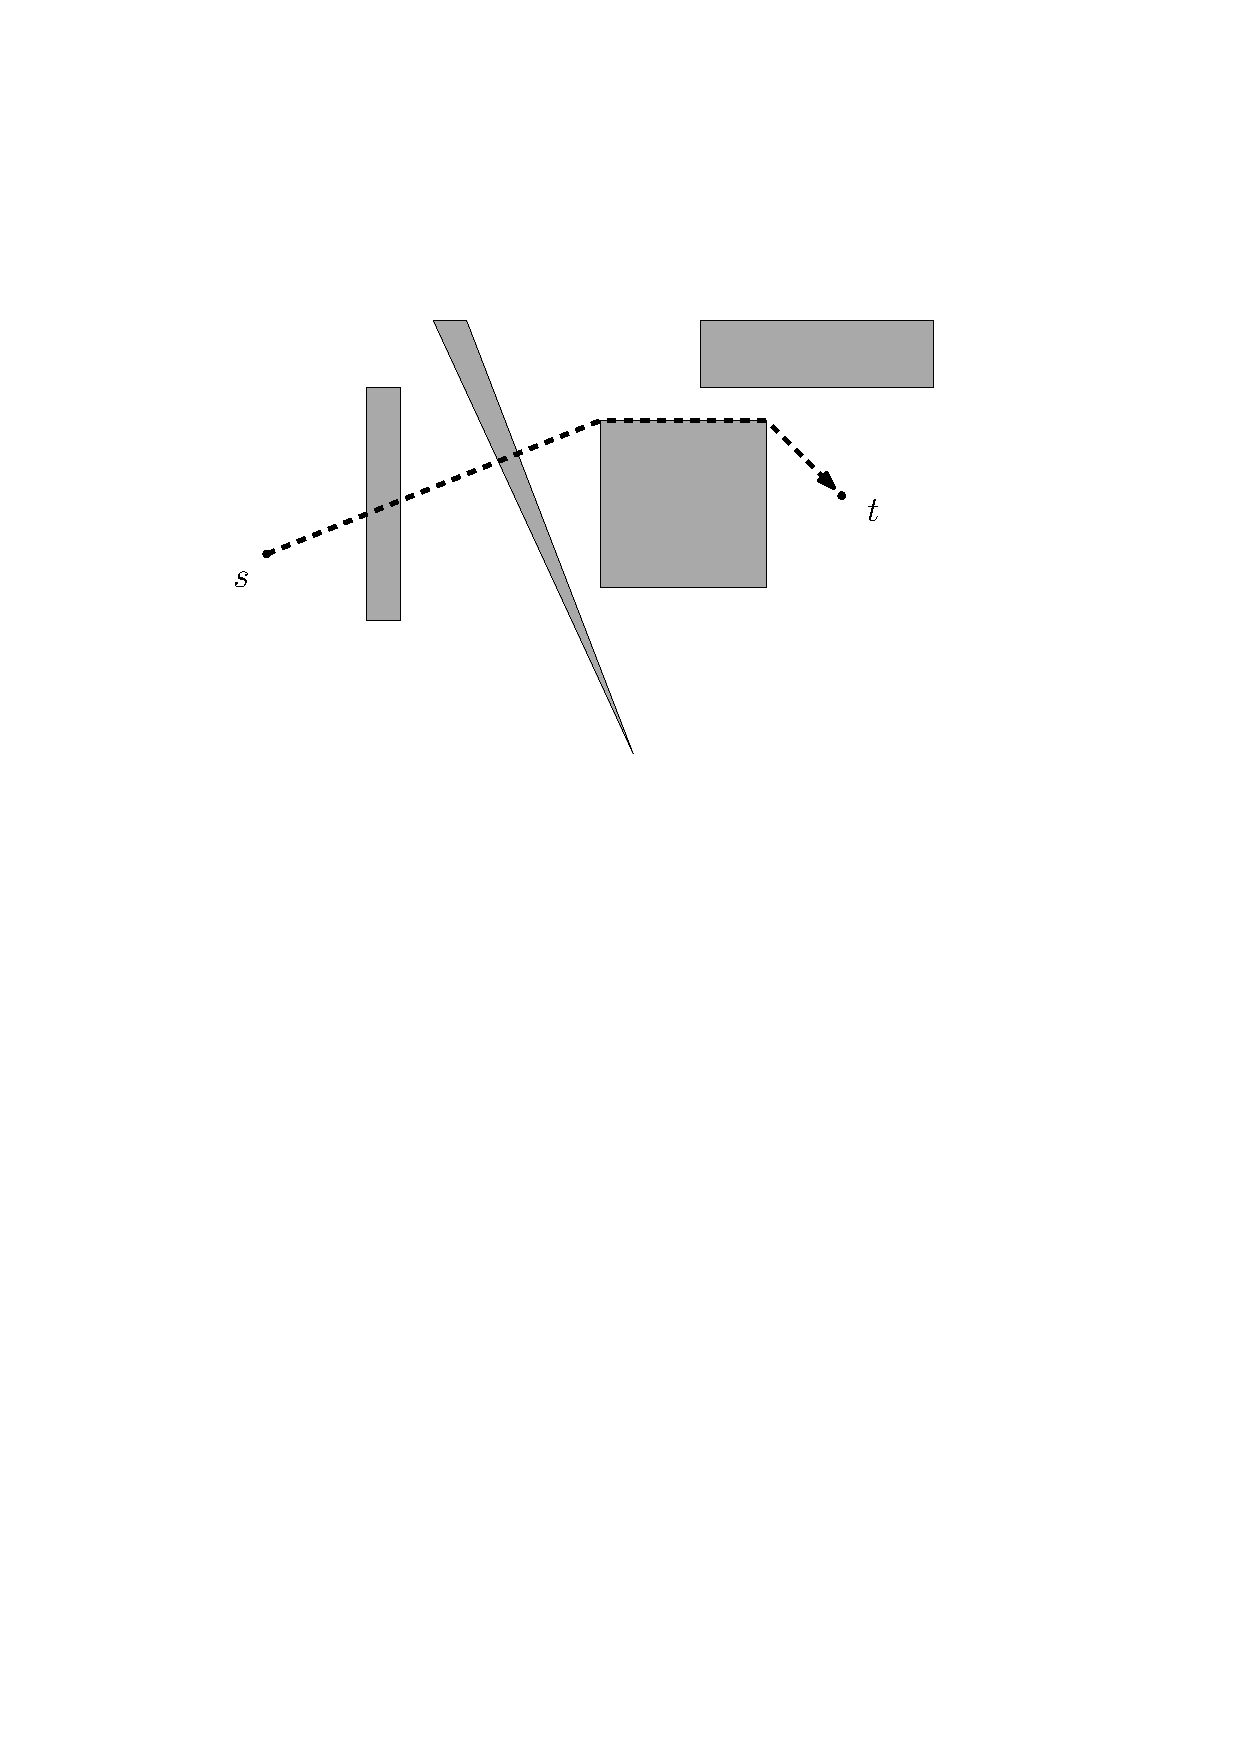
\includegraphics[width=0.7\textwidth]{figures/shortestkpath.pdf}
	\caption{A shortest $k$-path from $s$ to $t$ with $k = 2$}
     \label{fig:shortestkpath}
\end{figure}

The problem lies in which polygons you should pass through to minimize the distance from
$s$ to $t$. They presented an $O(k^2 n\log n)$ algorithm for this problem,
which used a modified version of the 1999 algorithm\cite{HershbergerKS17}.
Notice that if $k = 0$ it is identical to the Shortest path with no violations.

In this thesis we are going to present implementation details of both the original
and the generalized problem. We start by describing and implementing a naive algorithm 
for solving the problem based on computing a visibility graph and then running the Dijkstra
single source shortest path algorithm. Afterwards we are going to explain the theoretical
results leading to the algorithm and the implementation details. Lastly we describe the 
algorithm from 2017 and its implementation details.

\section{Formal Problem description} 
\label{problemdescription}
Given two points in the plane $s,t\in\mathbb{R}^2$ and a list of polygons
$\mathcal{O}=o_1,\dots,o_h$ where $o_i$ is a list of points in polygon $o_i$
starting at an arbitrary place and in clockwise order (note that sometimes we
use $\mathcal{O}$ as a set e.g. polygon $o_i \in \mathcal{O}$). We say a
\emph{legal path} is a list of points where two adjacent points are mutually
visible, i.e. you are able to draw a line from one to the other without
crossing the interior of any polygon in $P$.  We want to find a shortest legal
path from $s$ to $t$.

\section{Previous work}
\begin{table}[H]
\begin{tabular}{ c l l l c c} 
	\hline
	Year & Paper & Run time & Space & Visibility graph & SPM \\
	\hline
	 & Naive\tablefootnote{See Chapter 2} & $O(n^3)$ & $O(|E|)$ & x &\\

	1978 & Lee \cite{LEE78}\tablefootnote{We were not able to obtain the
	original ph.d. thesis, the got the running time from \cite{HershbergerS99} }
	& $O(n^2\log n)$ & ? & x & \\

	1985 & Welzl \cite{DBLP:journals/ipl/Welzl85} & $O(n^2)$ & $O(n^2)$ & x & \\

	1991 & Ghosh et al. \cite{GhoshM91}\tablefootnote{Where $E$ is the number of
	edges in the visibility graph} & $O(E+n\log n)$ & $O(E+n)$ & x & \\

	1991 & Mitchell \cite{DBLP:journals/amai/Mitchell91}\tablefootnote{Where $k$
	is a number bounded by the number of different obstacles that touches any
	shortest path from $s$} & $O(kn \log^2 n)$ & $O(n)$ & & x\\

	1996 & Mitchell \cite{DBLP:journals/ijcga/Mitchell96}\tablefootnote{For any
	$\varepsilon>0$ where the constant in the big-Oh notion depending on
	$\varepsilon$ }& $O(n^{3/2+\varepsilon})$ & $O(n)$ & & x\\

	1999 & Hershberger et al. \cite{HershbergerS99} & $O(n\log n)$ & $O(n\log
	n)$ & & x\\
	\hline
\end{tabular}
\caption{Shortest Paths in the Plane with Polygon obstacles algorithms}
\end{table}

In 1978 Lee presented a $O(n^2\log n)$ algorithm for constructing a visibility
map in his Ph.d.  thesis\cite{LEE78}, we couldn't find the original paper, the
running time is taken from \cite{HershbergerS99}. 

Seven years later, in 1985, Welzl \cite{DBLP:journals/ipl/Welzl85} published a
$O(n^2)$ time algorithm consuming $O(n^2)$ for construction of a visibility
map.  

Six years later in 1991 Ghosh et al.\ \cite{GhoshM91} presented a $O(E+n\log n)$
algorithm consuming $O(E+n)$ space, for constructing a visibility graph where
$E$ is the number of edges in the visibility graph.
Since the visibility graph can contain $O(n^2)$ the algorithm is output bound
and people started making shortest path map algorithm insteed, hoping to reach
the $\Omega{(n\log n)}$ lower bound (see chapter \ref{chapter:lowerbound}).

That same year in 1991 Michell \cite{DBLP:journals/amai/Mitchell91} published
an algorithm for constructing the shortest path map, with running time
$O(kn\log^2 n)$ and $O(n)$ space consumption. Where $k$ is bounded by the
number of different obstacles that touches any shortest path from $s$.

In 1996 he improved the run time to $O(n^{3/2+\varepsilon})$, for any
$\varepsilon>0$ where the constant in big-Oh notion depends on $\varepsilon$
keeping the linear space consumption  \cite{DBLP:journals/ijcga/Mitchell96}.

Then finally in 1999 Hershberger et al.\ \cite{HershbergerS99} revealed a
$O(n\log n)$ algorithm for computing the shortest path map, matching the lower
bound. The space consumption is $O(n\log n)$ and it is still an open problem if
there exists an algorithm with run time $O(n\log n)$ and linear space
consumption.

%\section{Naive algorithm}
%Overview of naive
%\section{Hersberger suri}
%overview of hersberger suri

\section{Overview of thesis}
\begin{description}

	\item[Chapter 2] We descripe a simple $O(n^3)$ algorithm for contructing a
		visibility graph. Then we implement it and compare the run time to the
		theoratical time.

	\item [Chapter 3] Gives an overview of the Hershberger et al.
		\cite{HershbergerS99} algorithm.

	\item [Chapter 4] Goes through the formal definition of the shortest path
		maps and its geometric properties including the complexity of the map.

	\item [Chapter 5] Explaines what the conforming subdivision is and how it is
		contructed.

	\item [Chapter 6] Is dedicated to the wavefront propagation algorithm
		explaining how it works and its implementation details.

	\item [Chapter 7] Presents the Hershberger et al. \cite{HershbergerKS17}
		which shows how to extend the original algorithm to work with $k$
		violations.

	\item [Chapter 8] In here we prove the lower bound of the "shortest path in
		the plane with obstacles problem in The Algebraic Computation Tree Model.
		By making a reduction from number destinction to number sorting to
		shortest map in the plane with obstacles.

	\item [Chapter 9] We conclude the work we have done.

\end{description}


\chapter{Simple $O(n^3 +k n^2)$ implementation}
In this section we describe an $O(n^3+k n^2)$ implementation which solves the
"Shortest Paths in Plane with Obstacles Violations"-problem. Recall that $n$ is
the number of vertices in the polygons and $k$ is the number of polygon
violations allowed. In the first section we describe how we construct the
visibility graph. Imagine a plane with a starting point $s$, an end point $t$,
and $\mathcal{O}$ polygon obstacles, which is build of groups of connected points,
each representing an obstacle. A visibility graph is a graph where for each set of
points $p,q\in \mathcal{O} \cup \{s,t\}$  there is an edge between them if the 
two points can see each other
without going (or looking) through any interior of an obstacle (see figure
\ref{visibilitygraph}). In the second section we explain Dijkstra's algorithm
for finding the shortest path from $s$ to $t$ in the visibility graph and
finally in the third section we test our implementation to compare if the actual 
running time is the same as the theoretical.

\begin{figure}[H]
	\begin{subfigure}{.5\textwidth}
		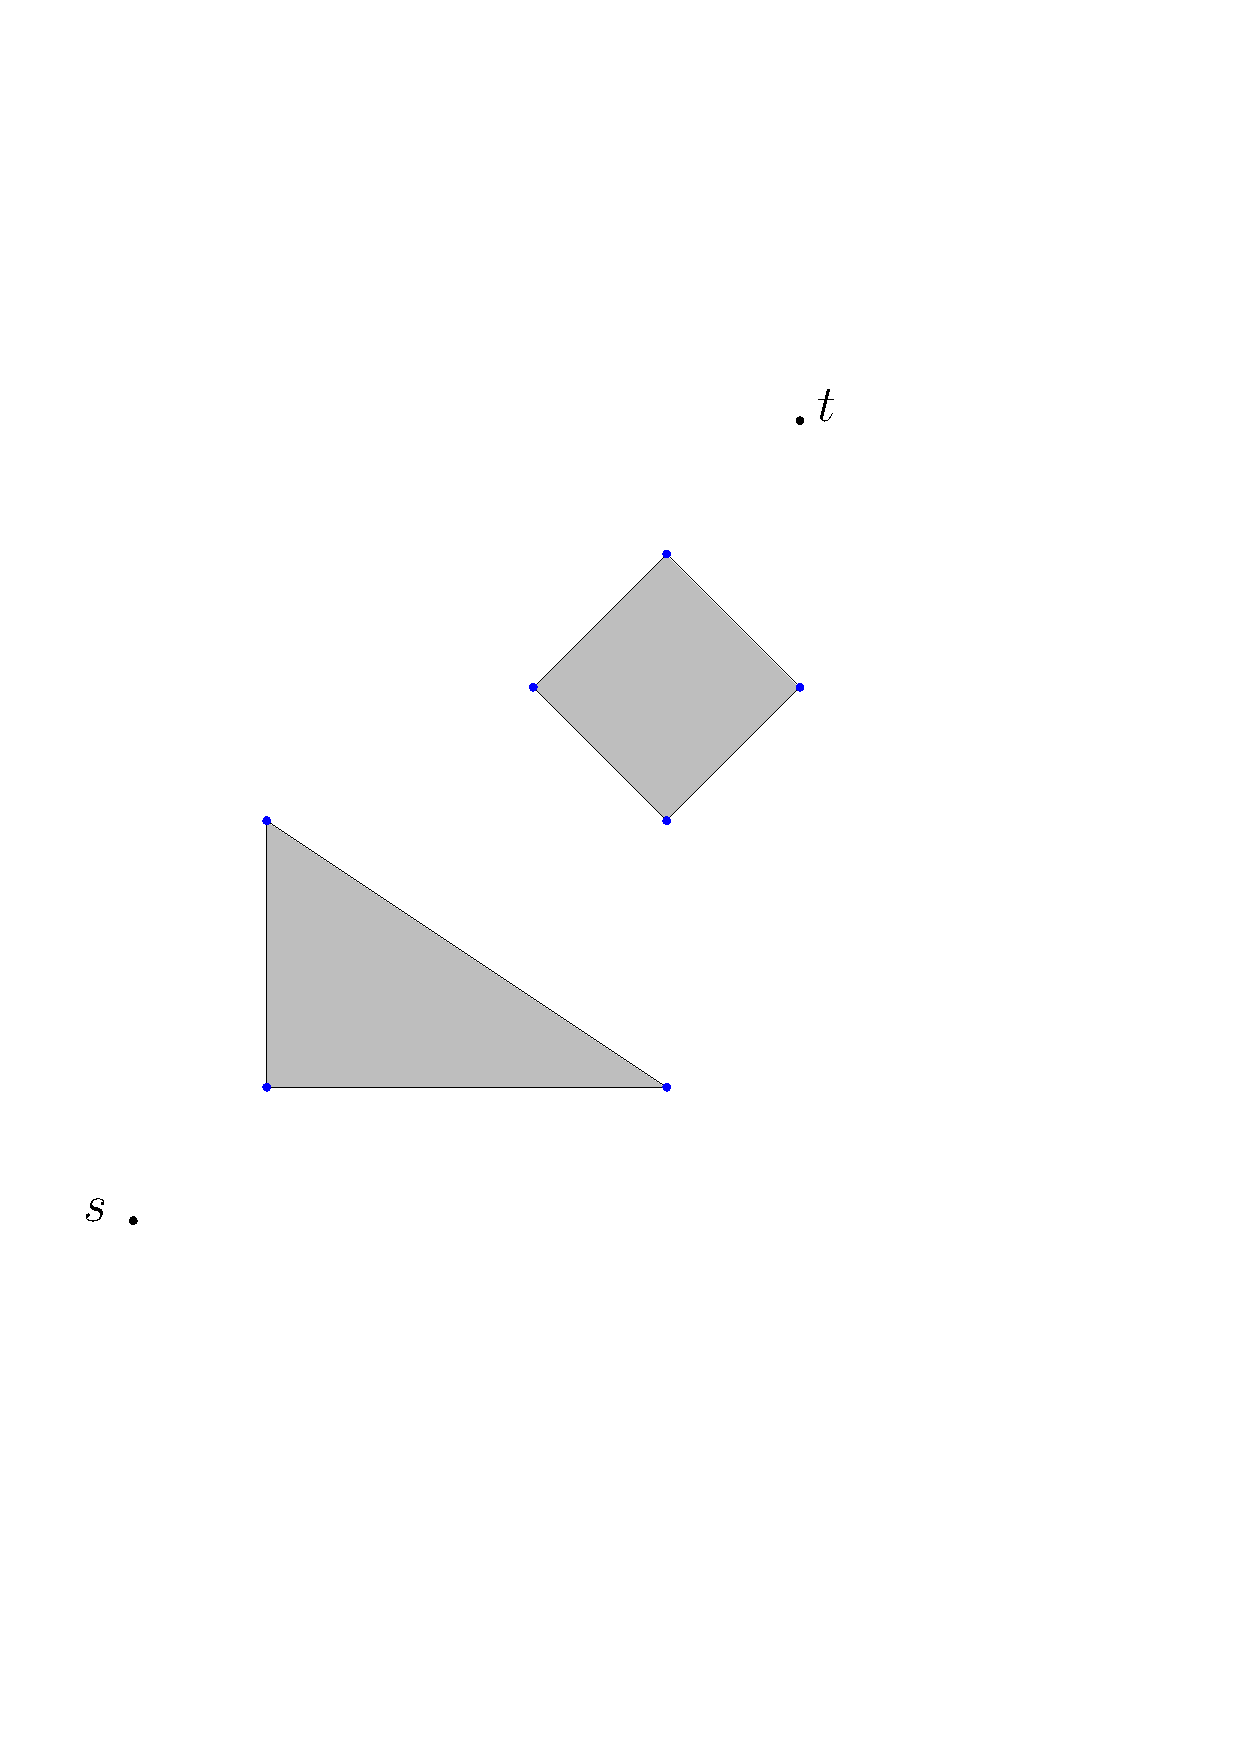
\includegraphics[width=6cm]{figures/visibilitygraph1.pdf}
		\caption{}
	\label{fig:visibilitygraph1}
	\end{subfigure}
	\begin{subfigure}{.5\textwidth}
		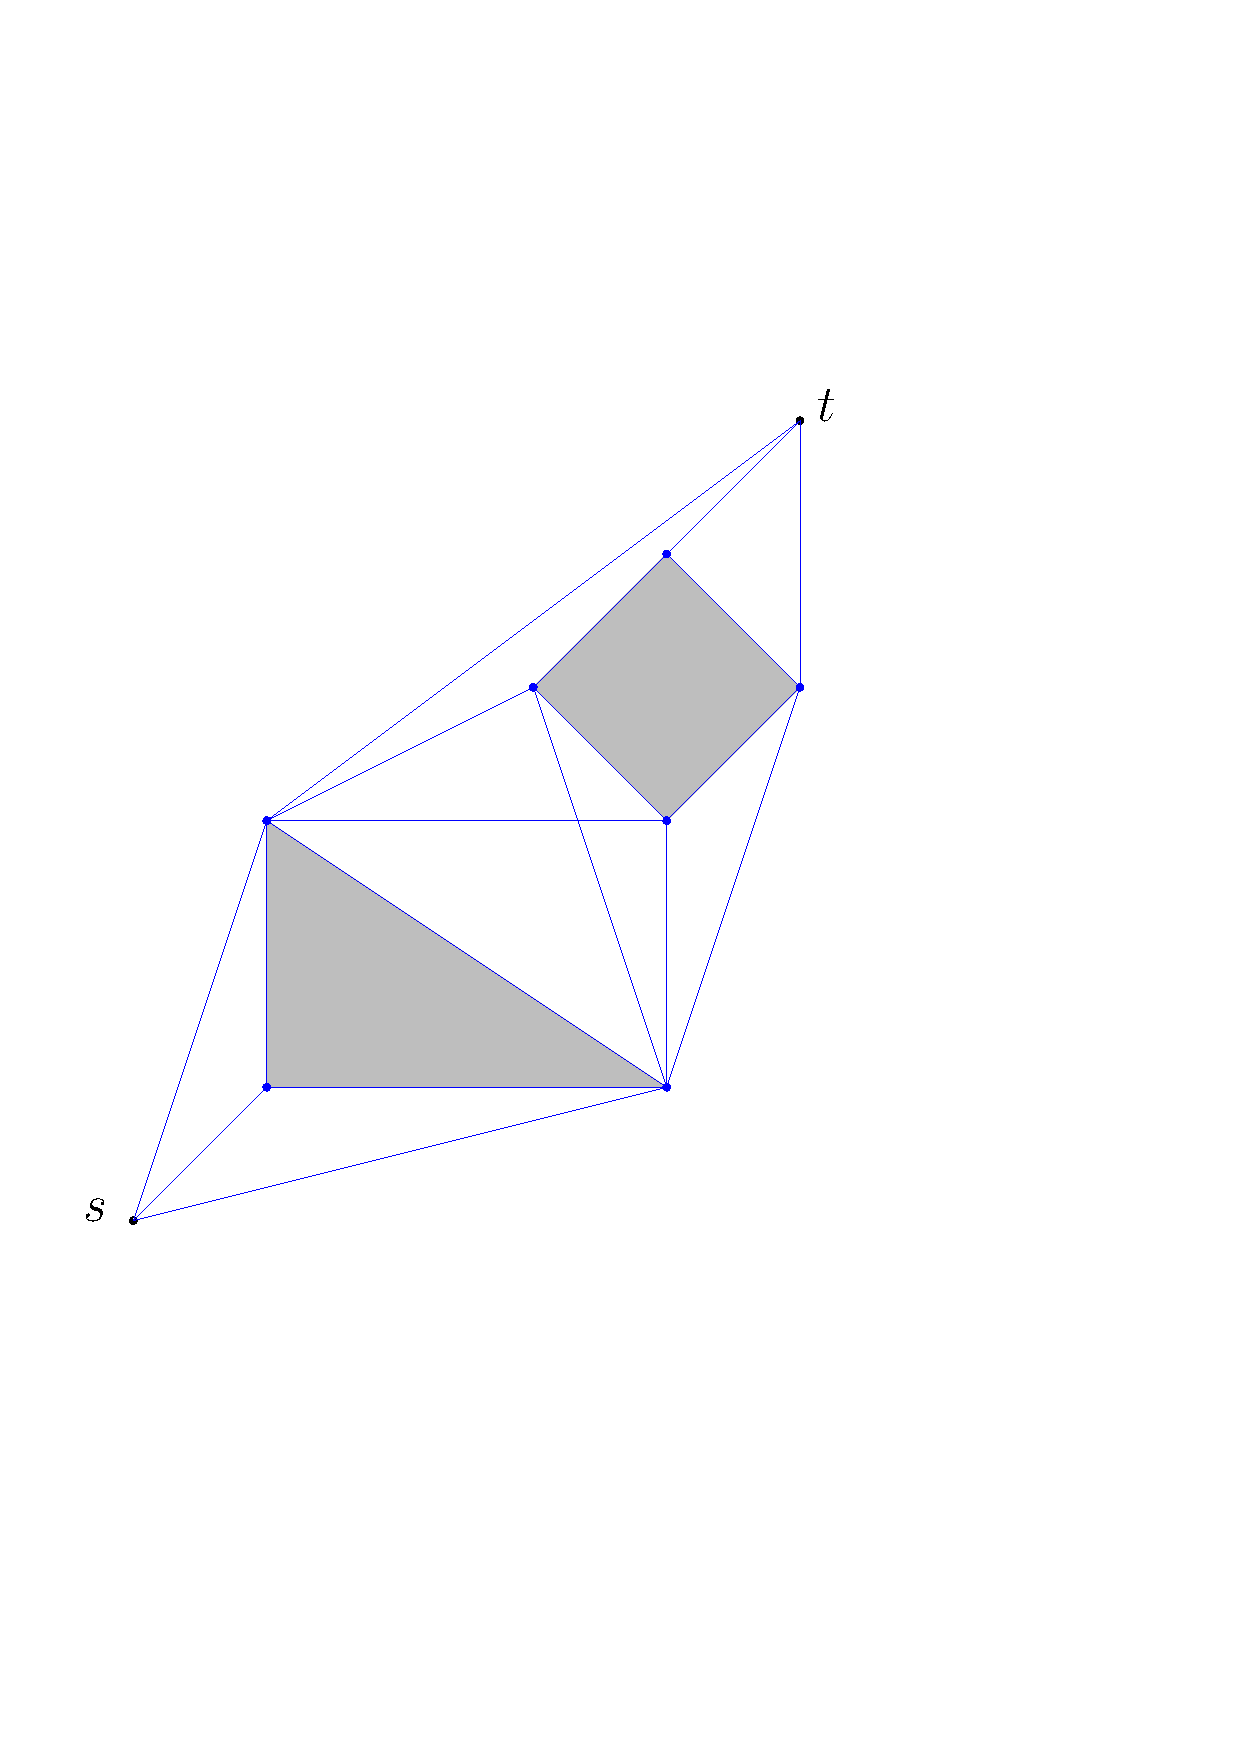
\includegraphics[width=6cm]{figures/visibilitygraph.pdf}
		\caption{}
		\label{fig:visibilitygraph2}
	\end{subfigure}
	\caption{Example of visibility graph}
	\label{visibilitygraph}
\end{figure}

\section{Constructing the visibility graph}
The naive way of constructing a visibility graph is to make a graph
where every set of points $p,q \in \mathcal{O} \cup \{s,t\}$ is connected to each other,
then removing all edges that crosses the interior of a polygon. But in this
setting we are allowed to cross $k$ polygons, so we construct the graph a bit
different. Given a set $\mathcal{O}$ consisting of all the polygons, where each polygon
is a list of the points in the polygon we use the following algorithm \ref{algo:MakeVisibilityGraph}.  
Create a graph $G_0=(V,E)$, where $V$ contains all the vertices in $P\cup \{s,t\}$,
and let $E$ contain all possible connections between the vertices. Make $k$
copies of the graph and name them $G_1,\dots,G_{k}$. Algorithm \ref{algo:MakeVisibilityGraph} goes as
follows: for each graph $G_i$, take each edge $e_j\in G_i$ and call
NumberOfCrosses$(e_j)$, which returns the number of polygons from $\mathcal{O}$ that the
line segment crosses, and connect the endpoint to the corresponding point in
$G_{i+m}$, i.e.\ if you take an edge in the graph, that goes through $m$
polygons, you travel $m$ graphs up. If $i+m > k$ then delete the edge. We now
have a graph that has $k$ levels where every time you go through $k$ polygons
you go $k$ levels up.

\begin{algorithm} 
	\caption{MakeVisibilityGraph($P,s,t$)}
	\begin{algorithmic}[1]
		\ForAll{$G_i=(V_i,E_i) \in G$}
		\ForAll{$e \in E_i$}
			\State $crosses = numberOfCrossings(e)$
			\If{$crosses+i<=k$}
				\State make $e$ go from $G_i$ to $G_{i+crosses}$
			\Else
				\State delete edge $e$
			\EndIf
		\EndFor
		\EndFor
	\end{algorithmic}
	\label{algo:MakeVisibilityGraph}
\end{algorithm}

The only missing part is the numberOfCrossings function, which we will define
below.

\subsection{Number of crossings}
Calculating the number of polygons a line segment crosses is no trivial task,
since there is a number of edge cases. We try to give a brief intuition of the
edge cases, and then present our algorithm.
The first five cases (a-e) in figure \ref{fig:crossings} are allowed intersections since
it is only the interior of a polygon that we can not travel. The
next five cases (f-j) are not allowed since they travel through the interior
of the polygon.

\begin{figure}
\begin{tabular}{|c|c|c|c|c|}
      \hline
		\multicolumn{5}{|c|}{No intersection} \\
		\hline
      \addheight{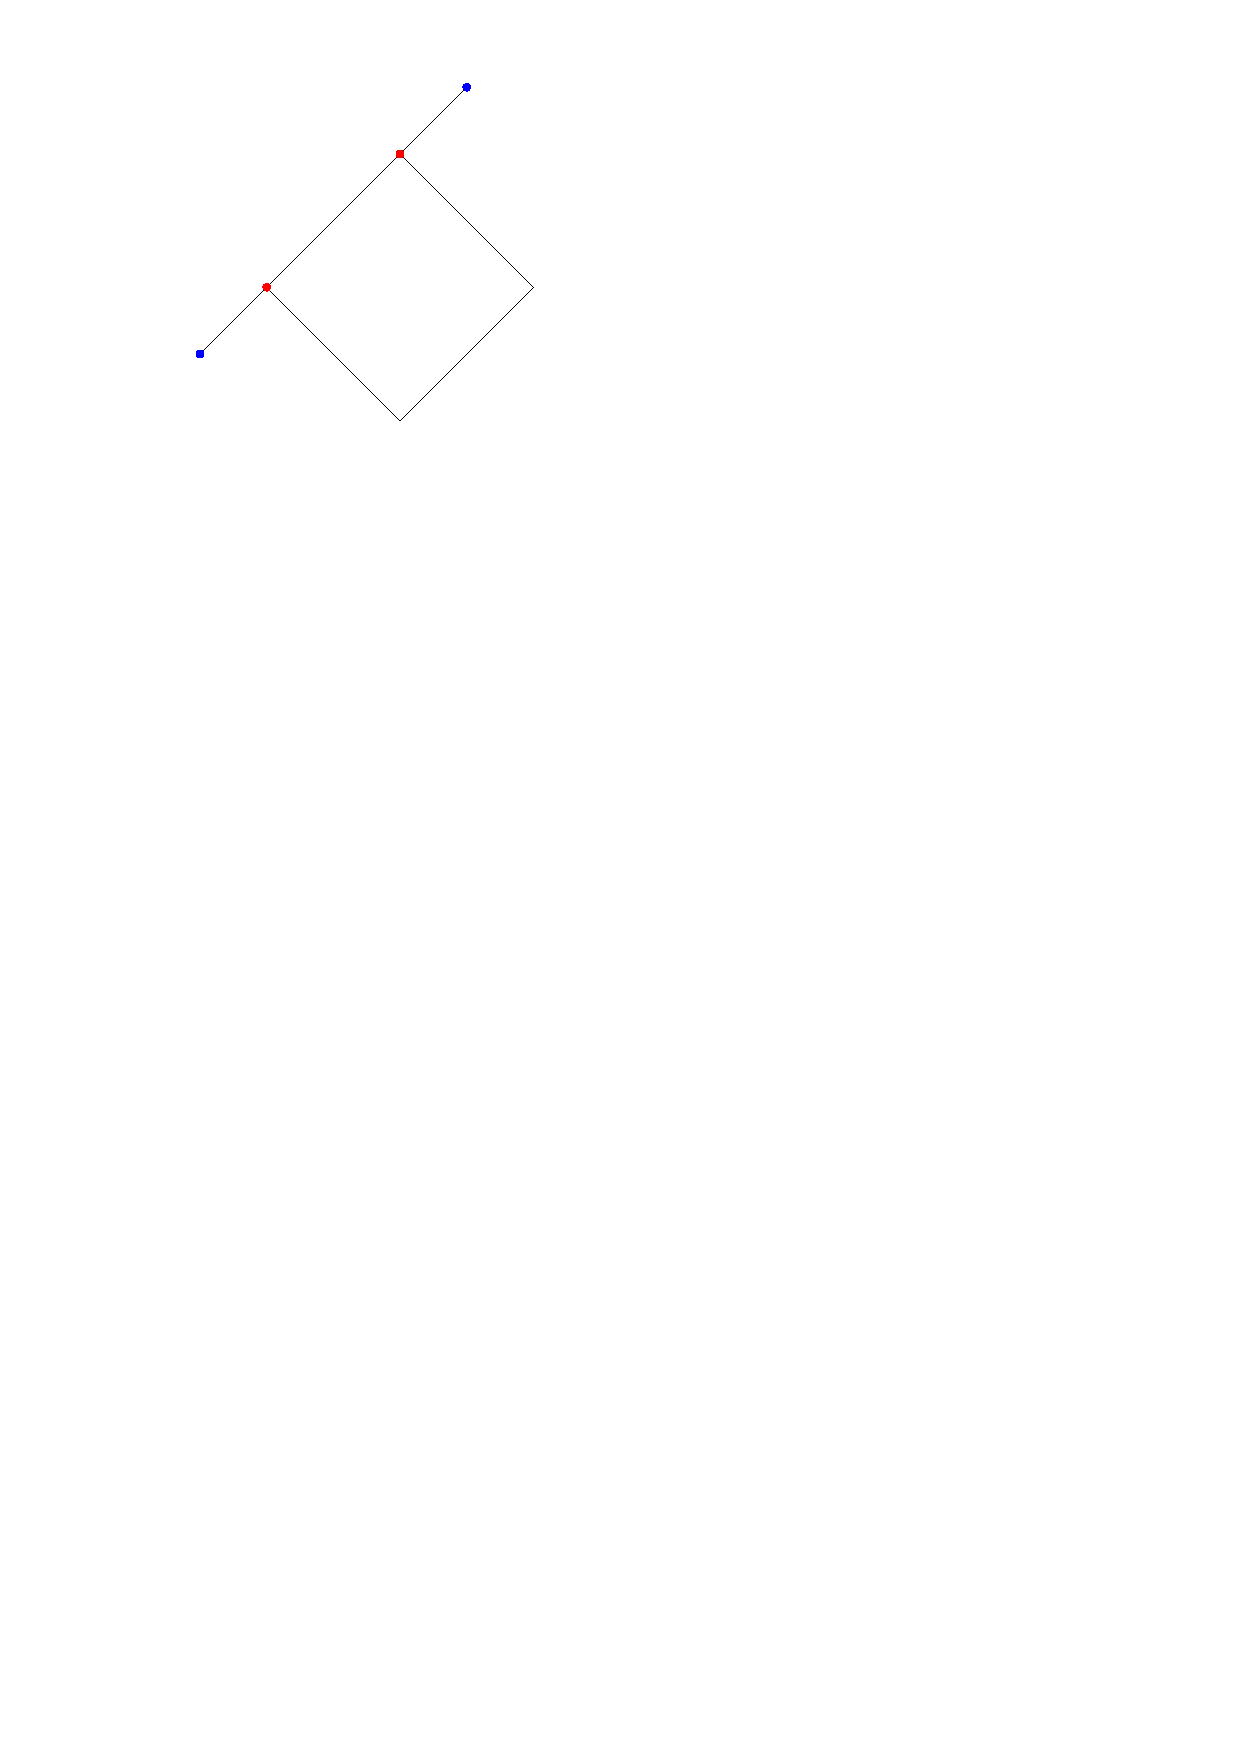
\includegraphics[width=20mm]{figures/crossFig1.pdf}} &
      \addheight{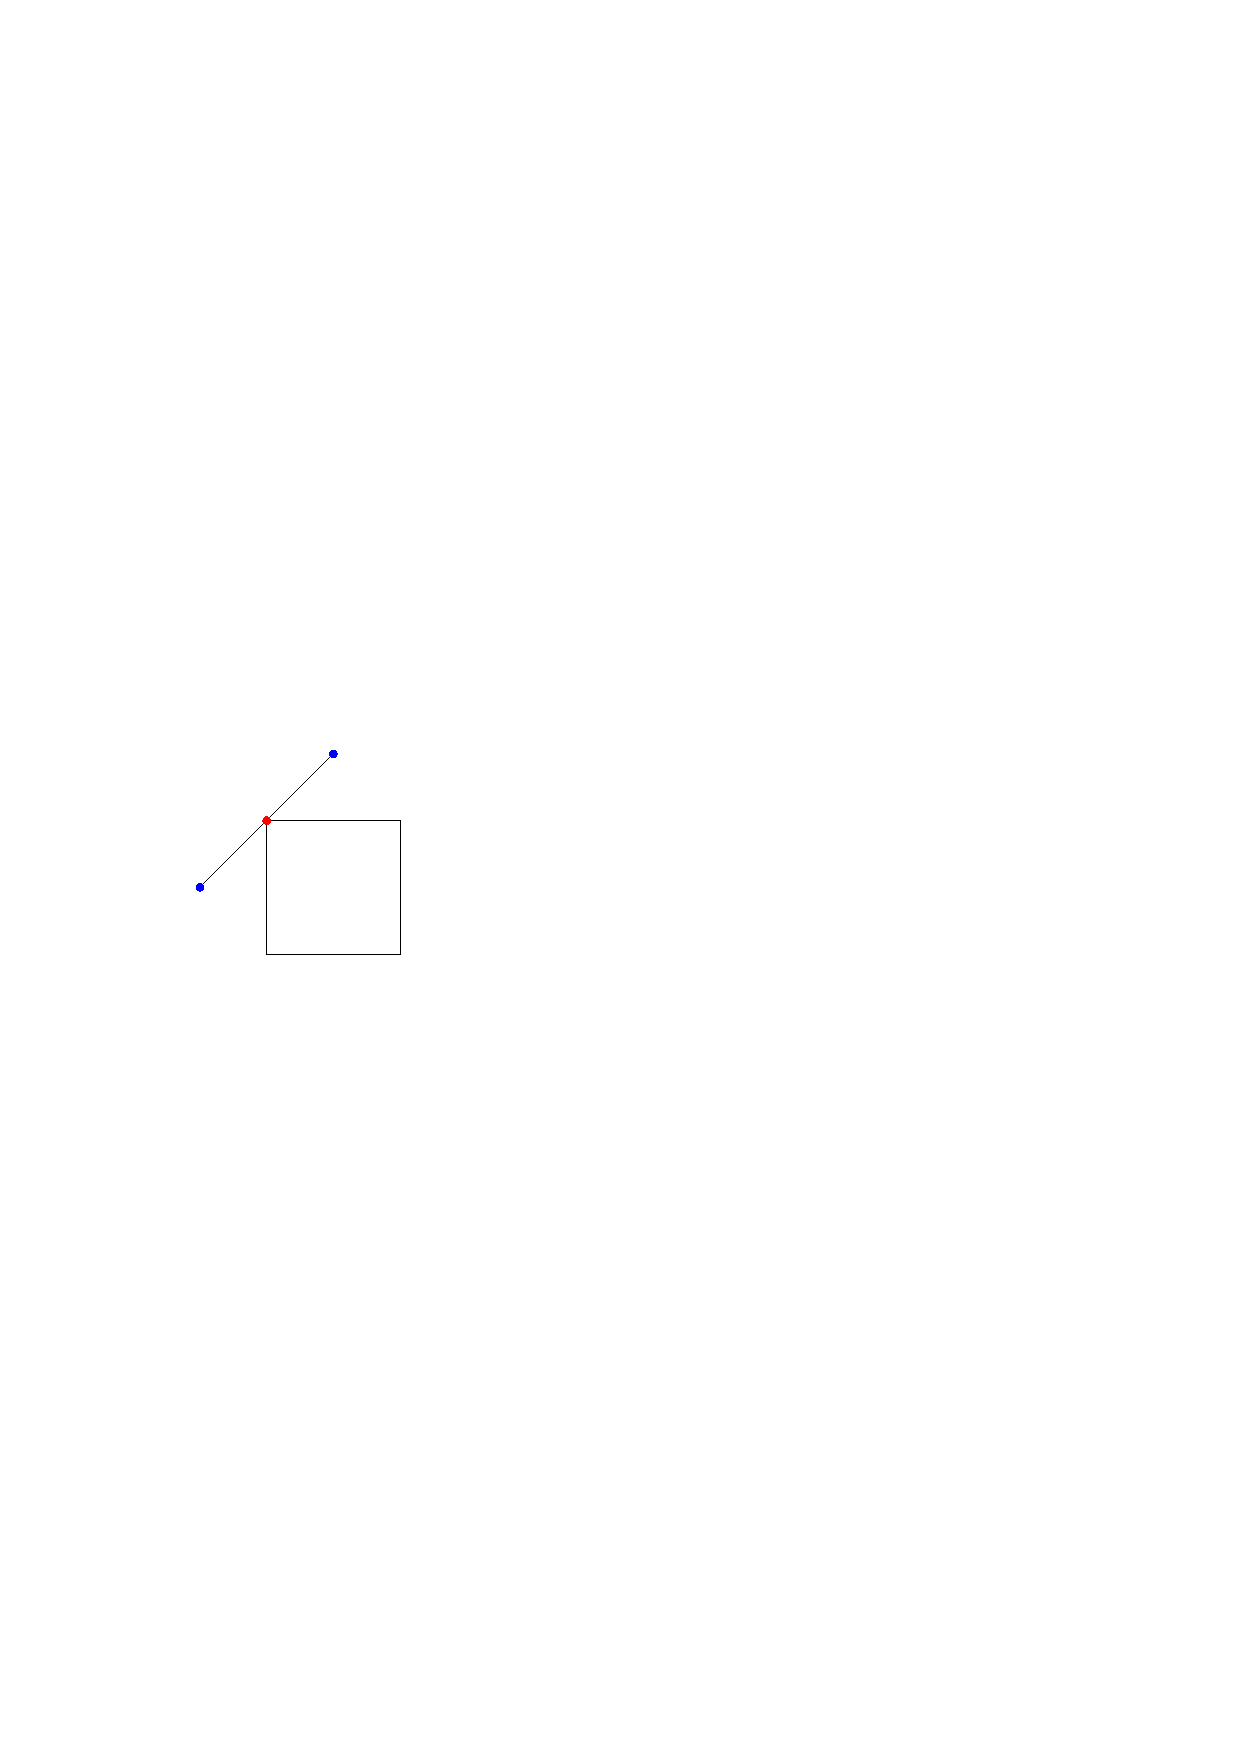
\includegraphics[width=20mm]{figures/crossFig2.pdf}} &
      \addheight{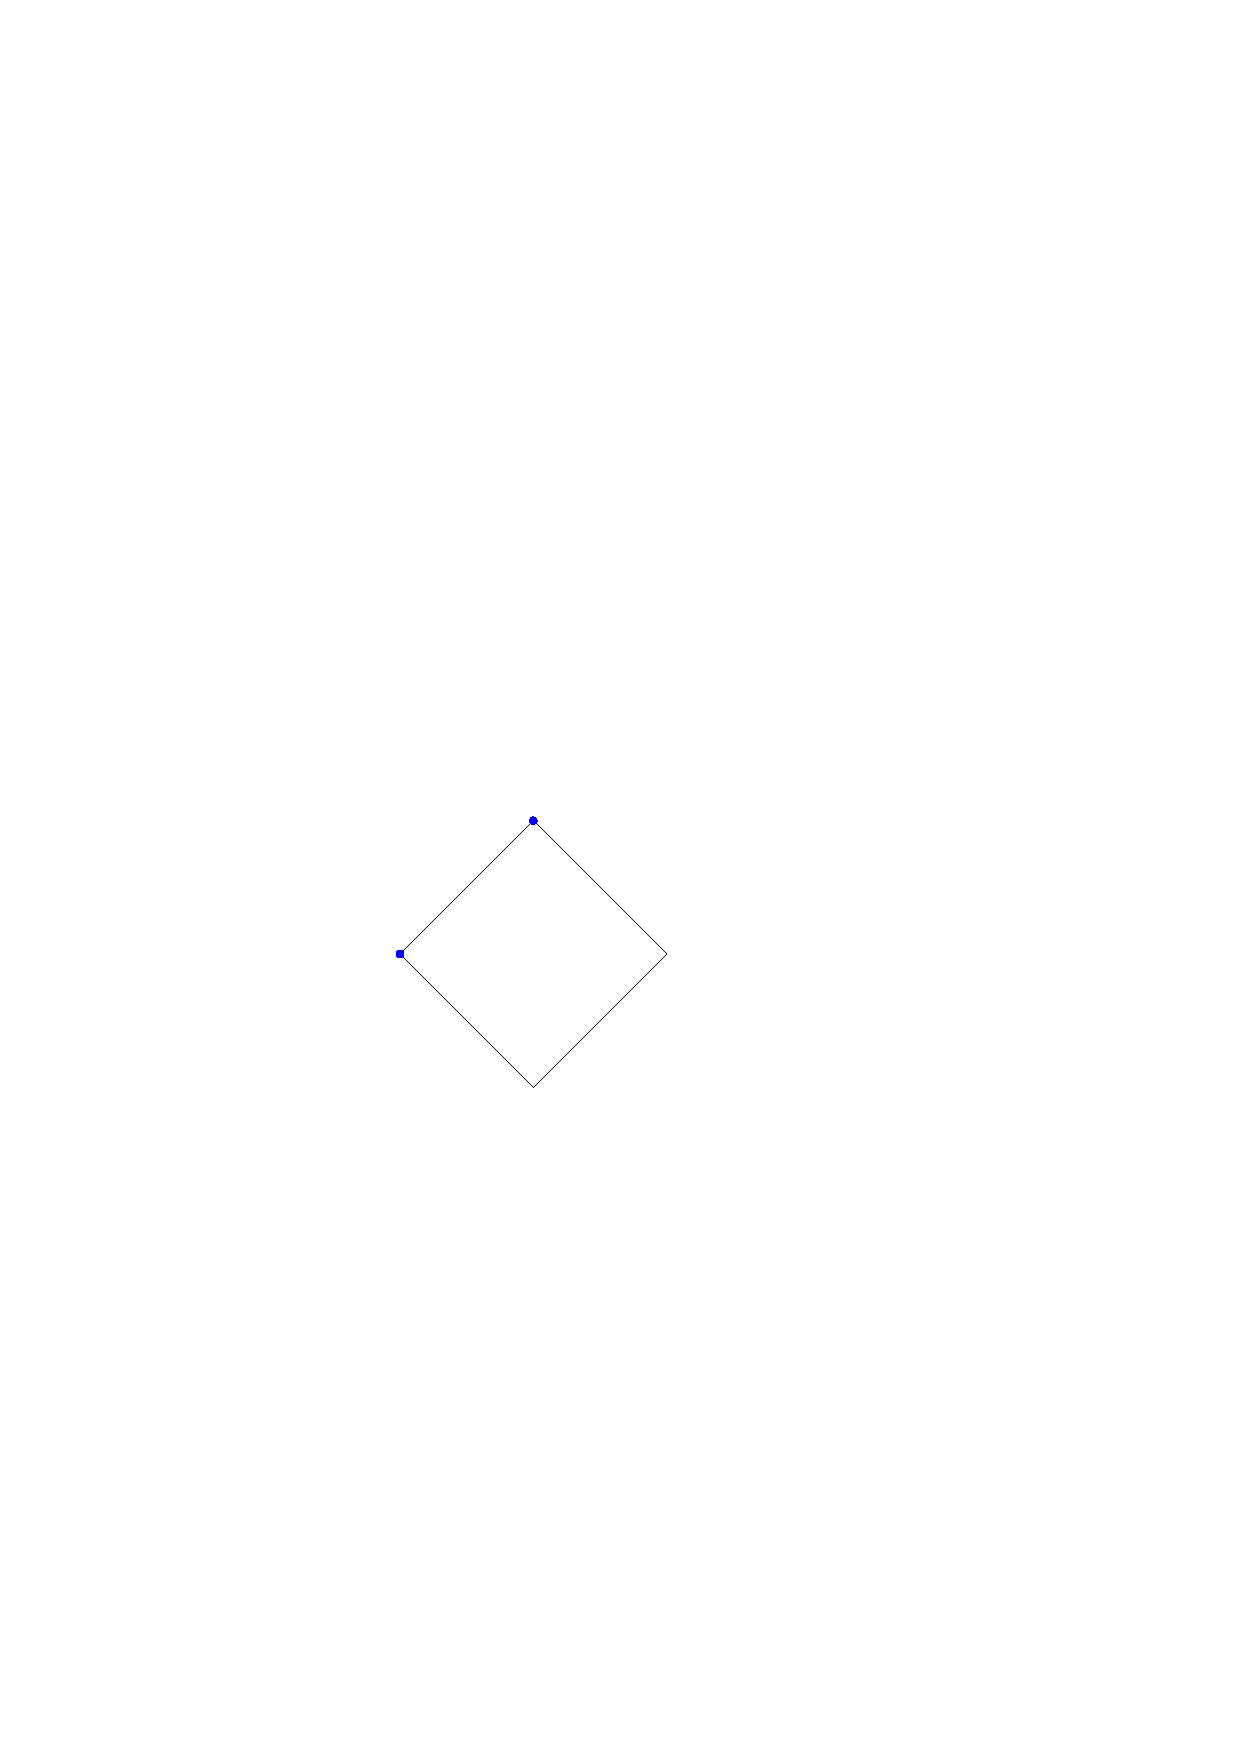
\includegraphics[width=20mm]{figures/crossFig3.pdf}} &
      \addheight{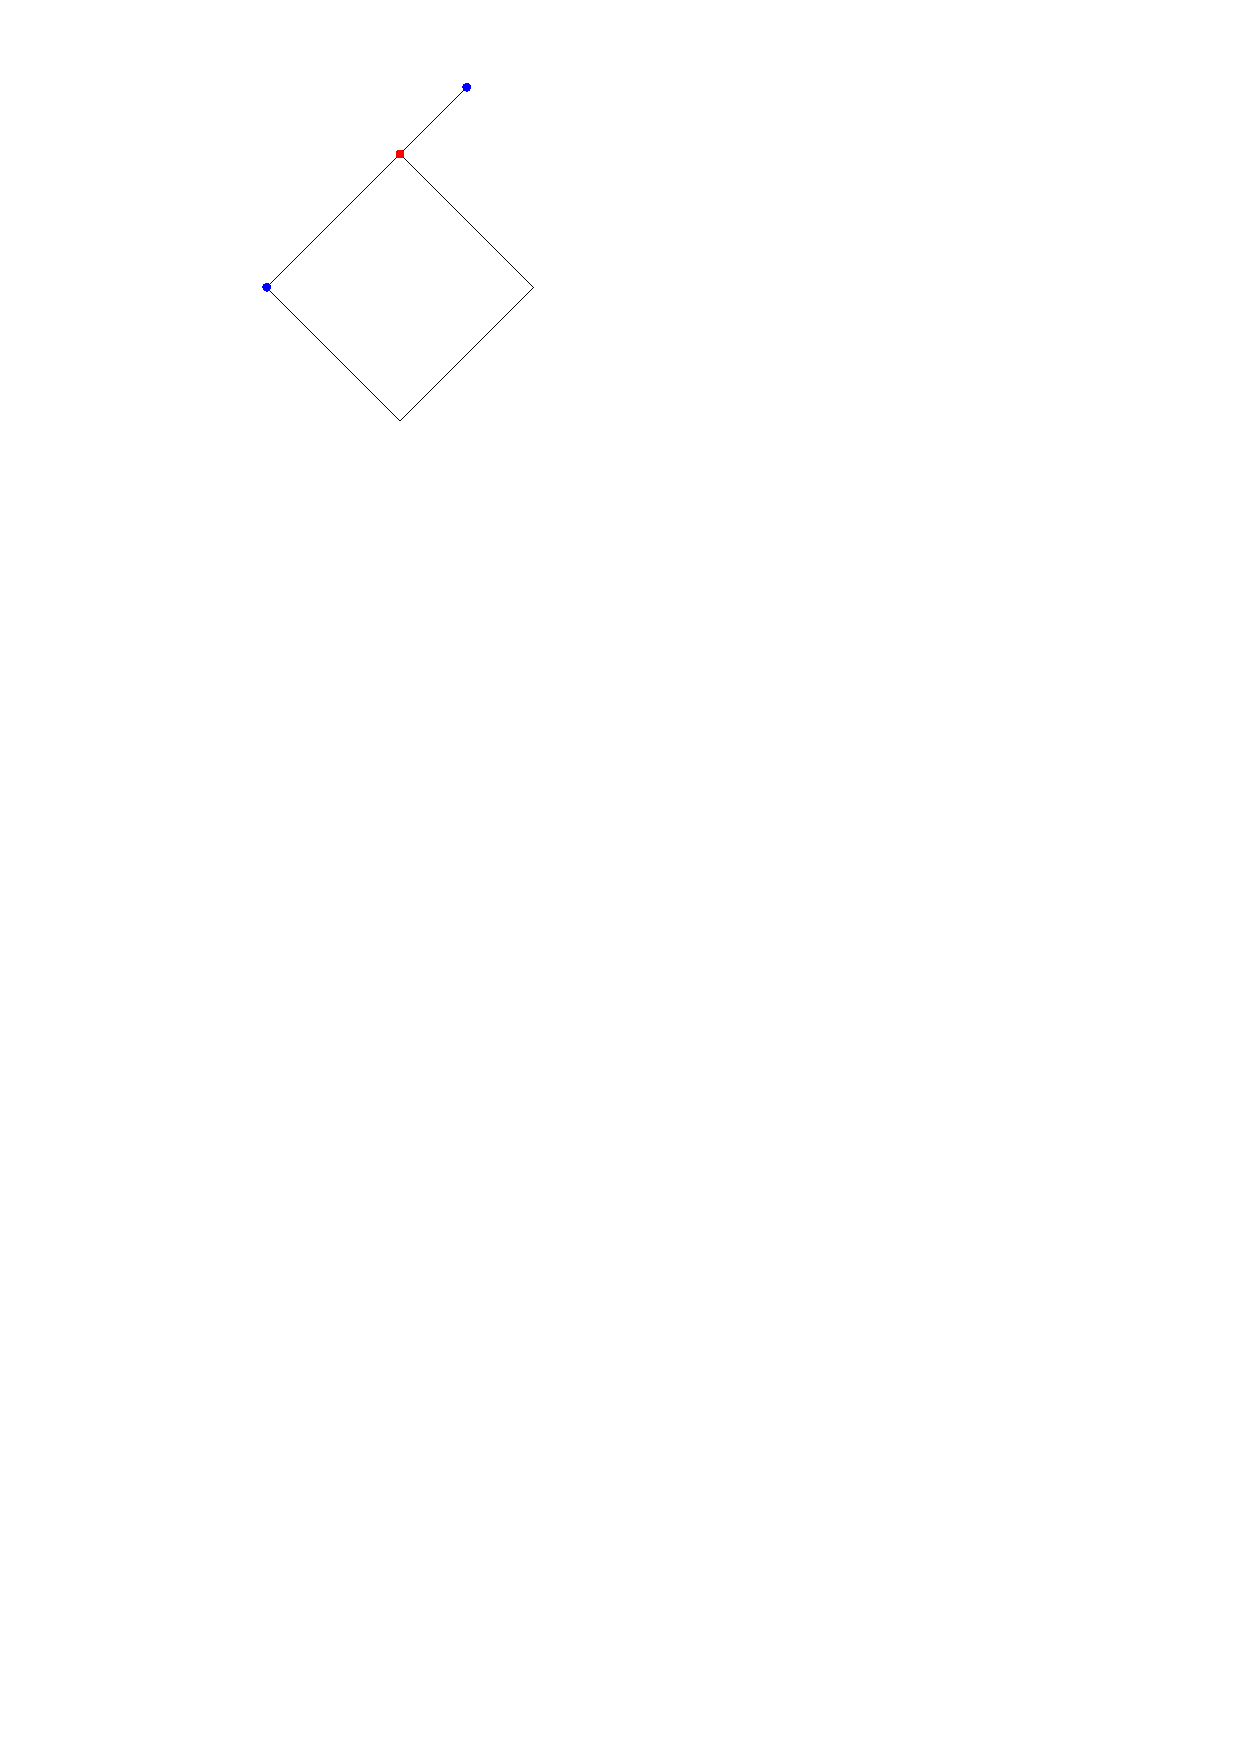
\includegraphics[width=20mm]{figures/crossFig4.pdf}} &
      \addheight{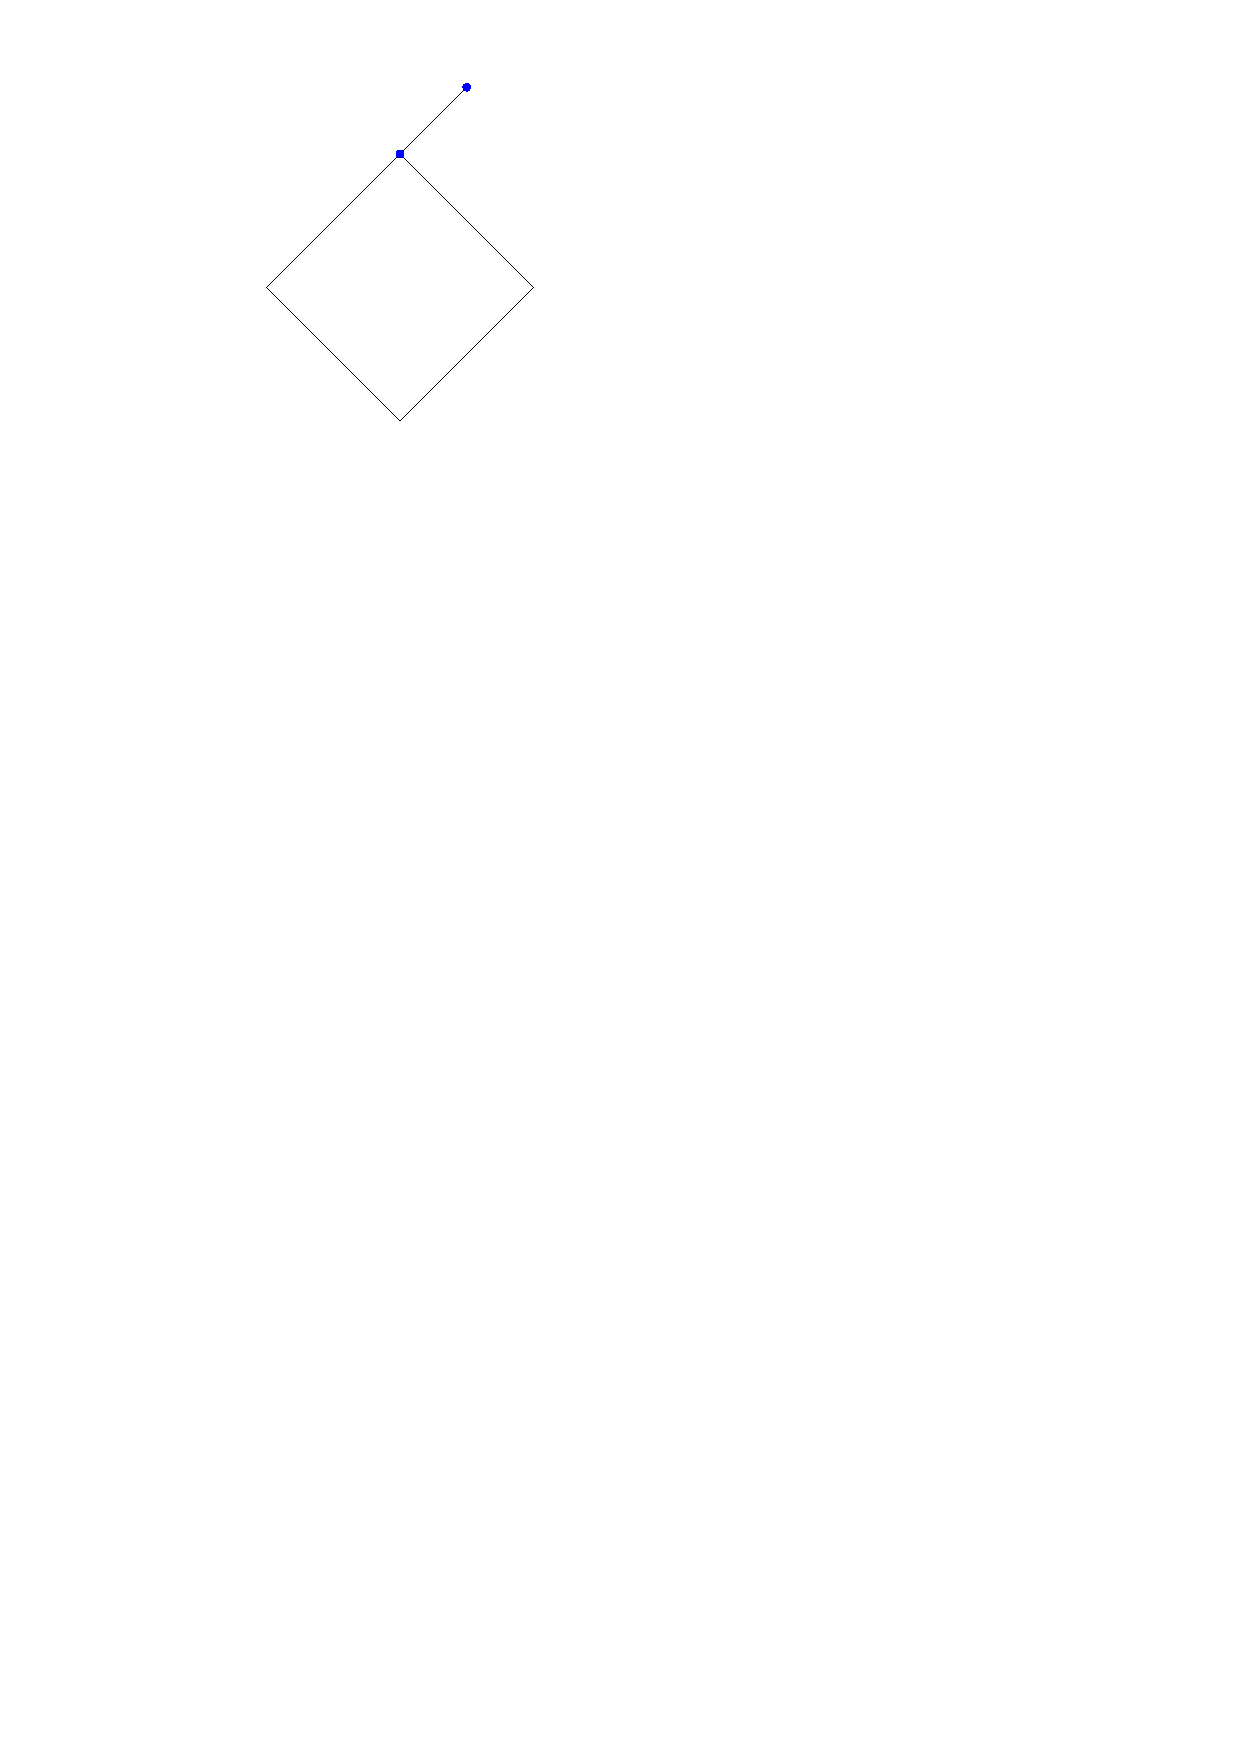
\includegraphics[width=20mm]{figures/crossFig5.pdf}} \\
      \small (a) &  (b) & (c) & (d) & (e) \\
      \hline
		\multicolumn{5}{|c|}{Intersection} \\
		\hline
      \addheight{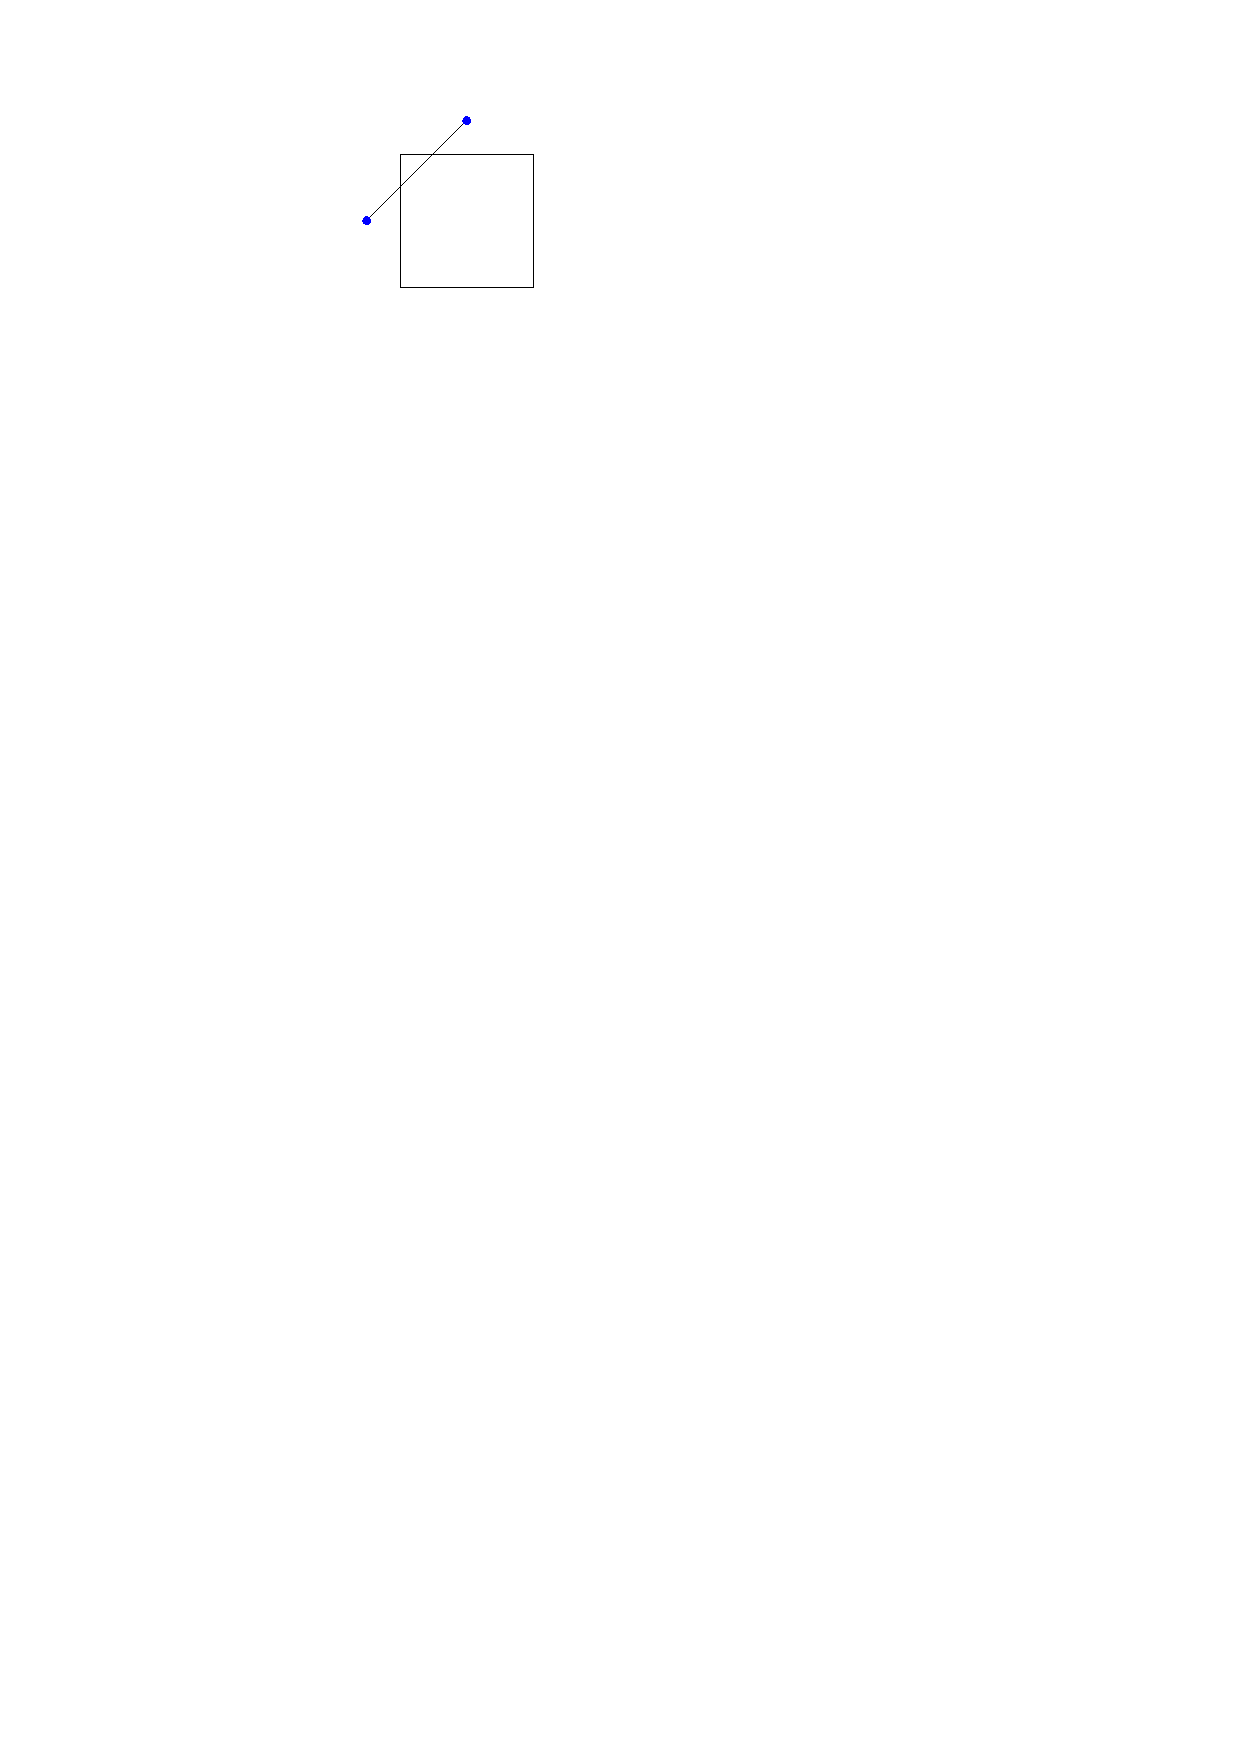
\includegraphics[width=20mm]{figures/crossFig6.pdf}} &
      \addheight{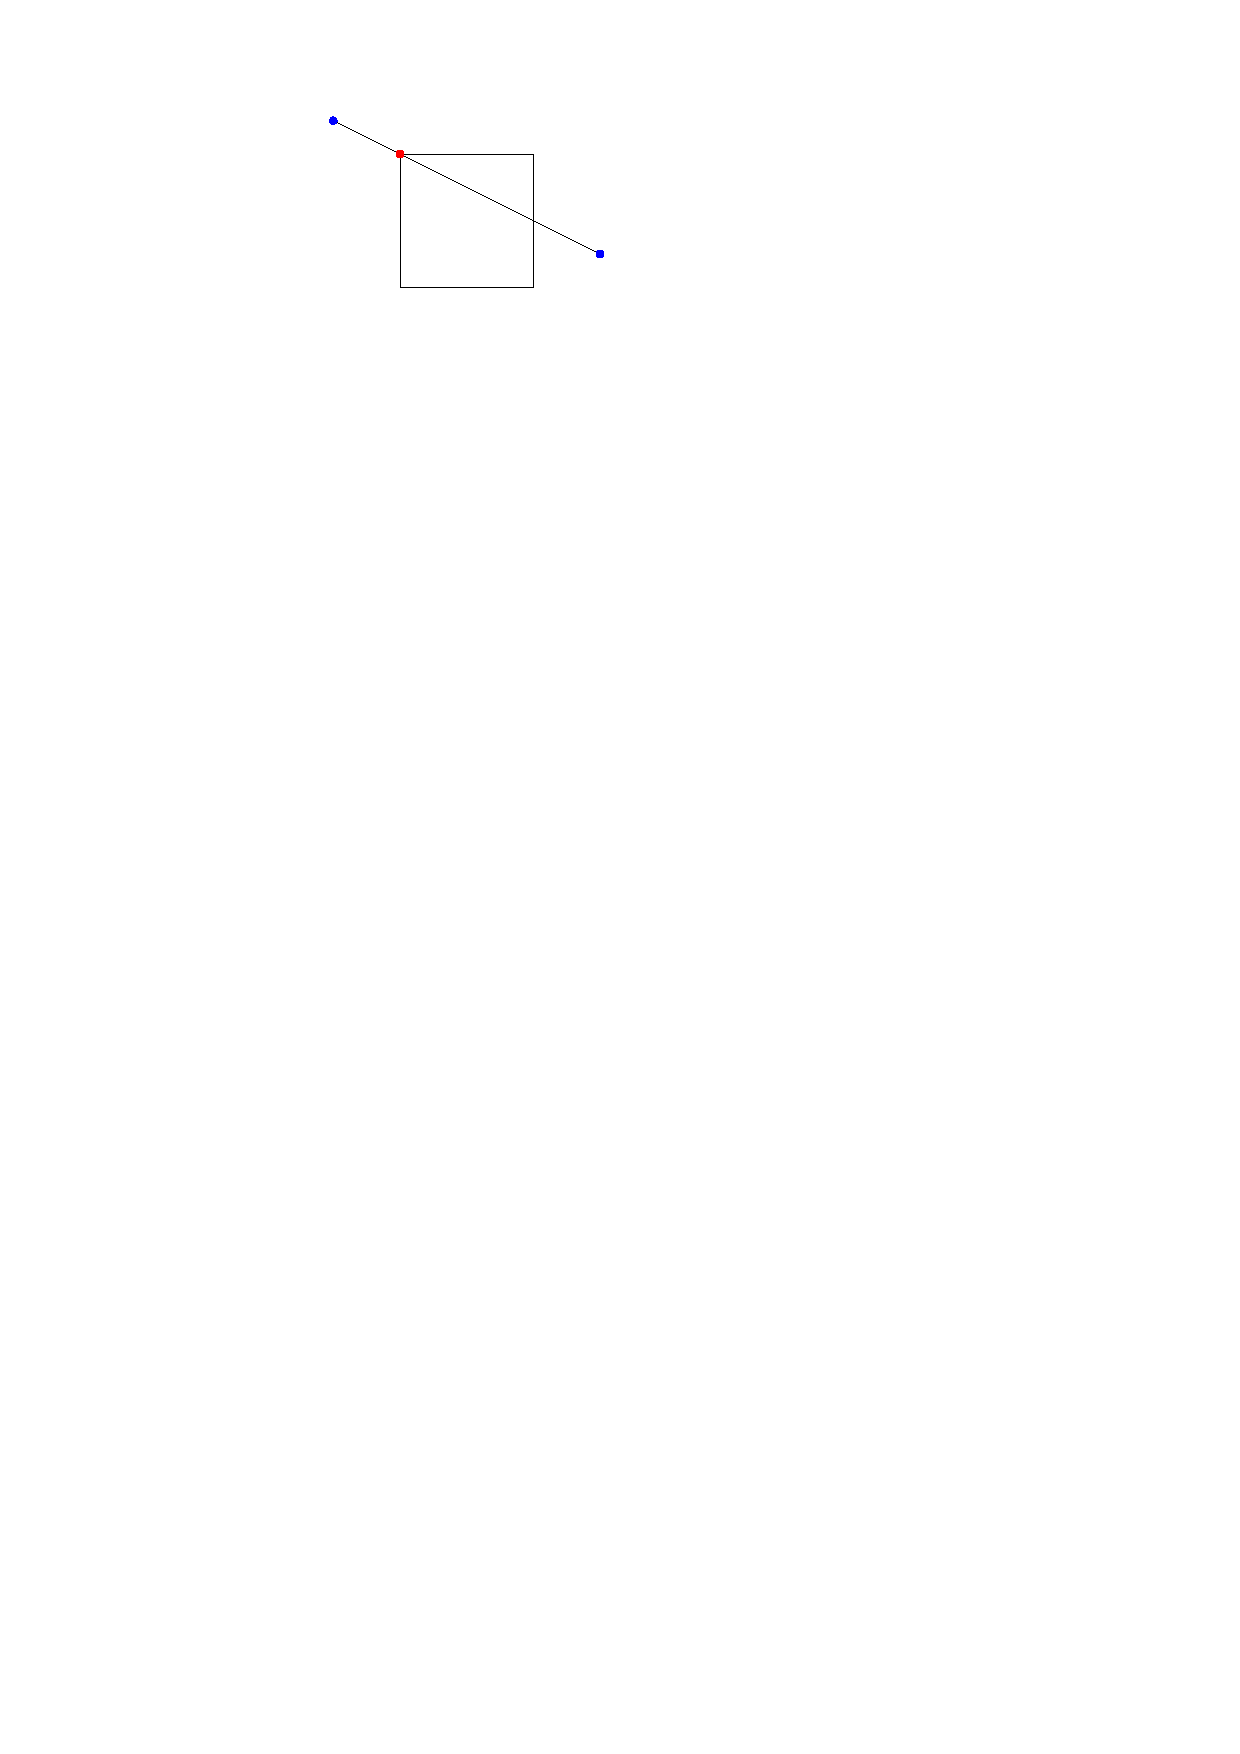
\includegraphics[width=20mm]{figures/crossFig7.pdf}} &
      \addheight{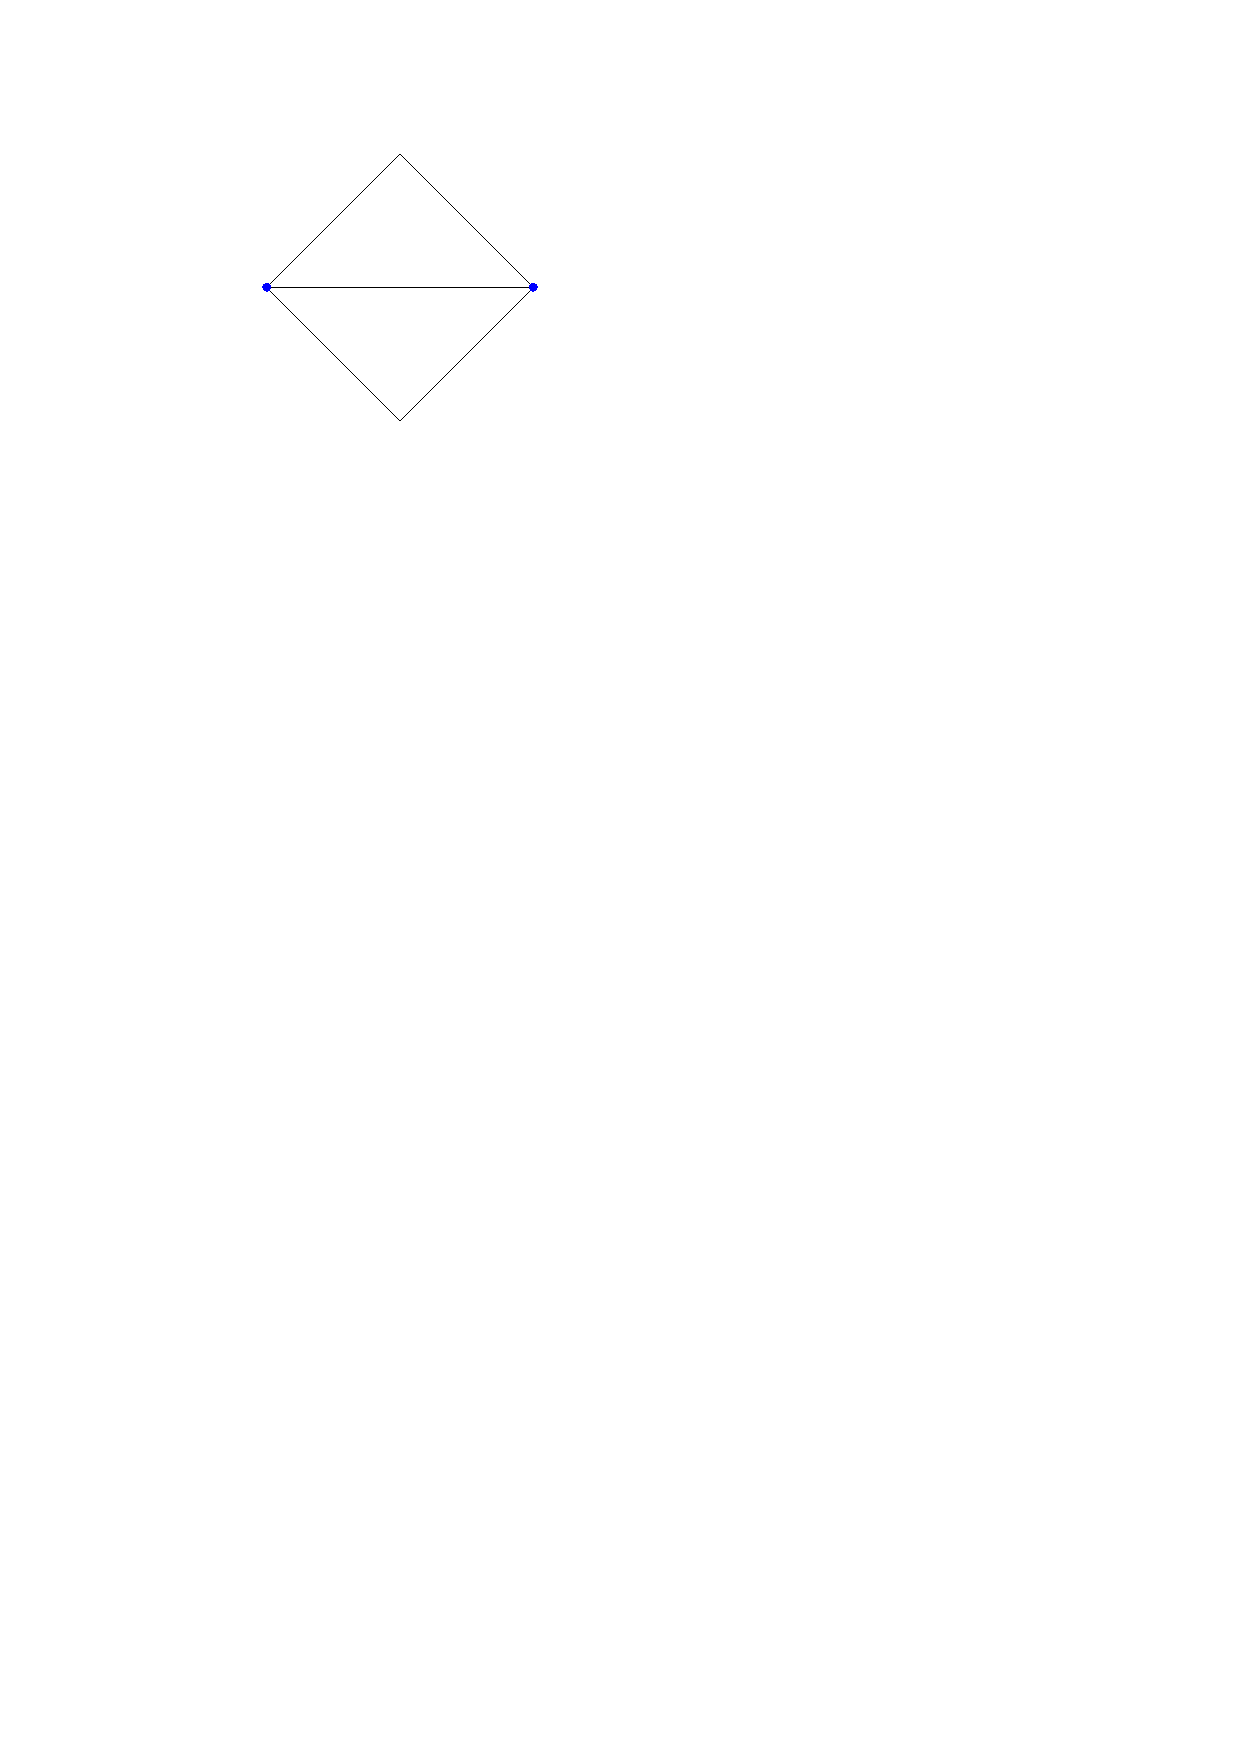
\includegraphics[width=20mm]{figures/crossFig8.pdf}} &
      \addheight{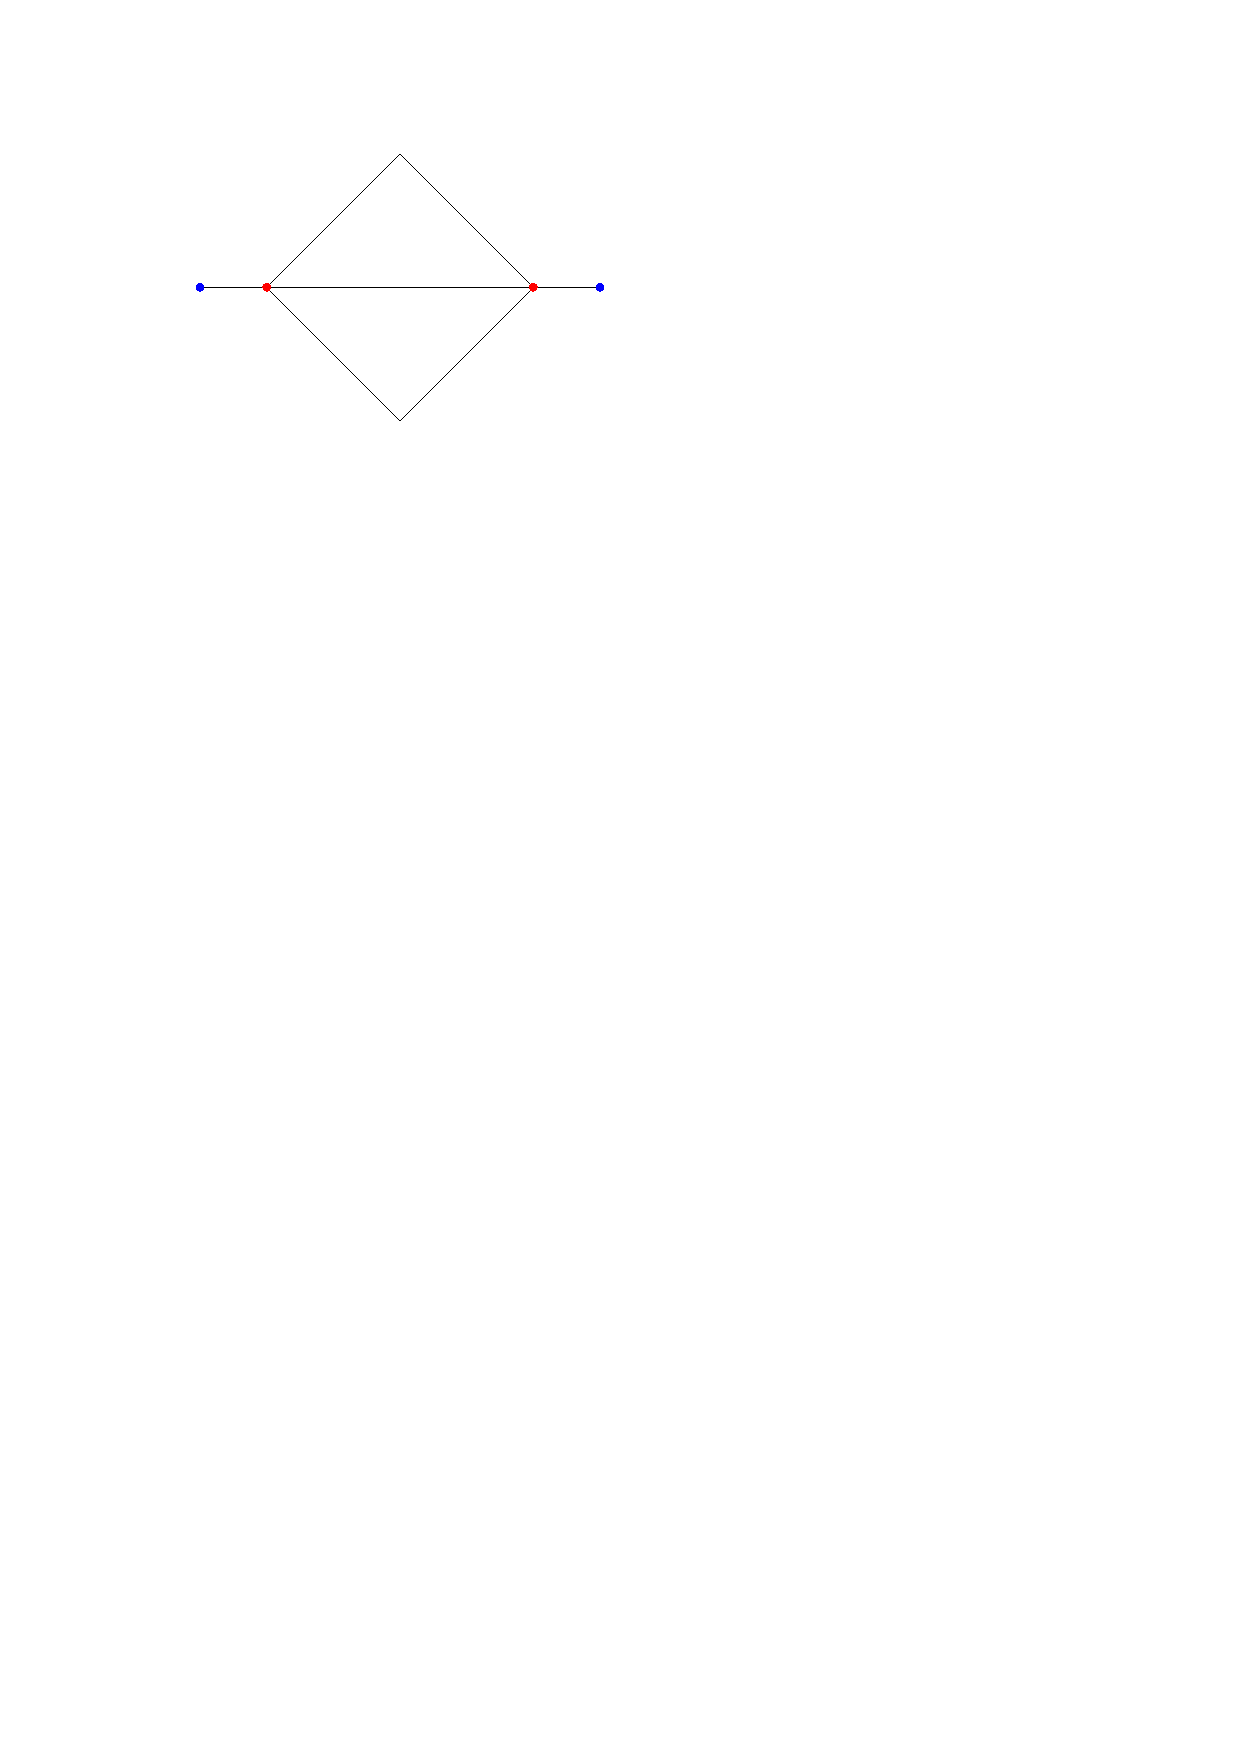
\includegraphics[width=20mm]{figures/crossFig9.pdf}} &
      \addheight{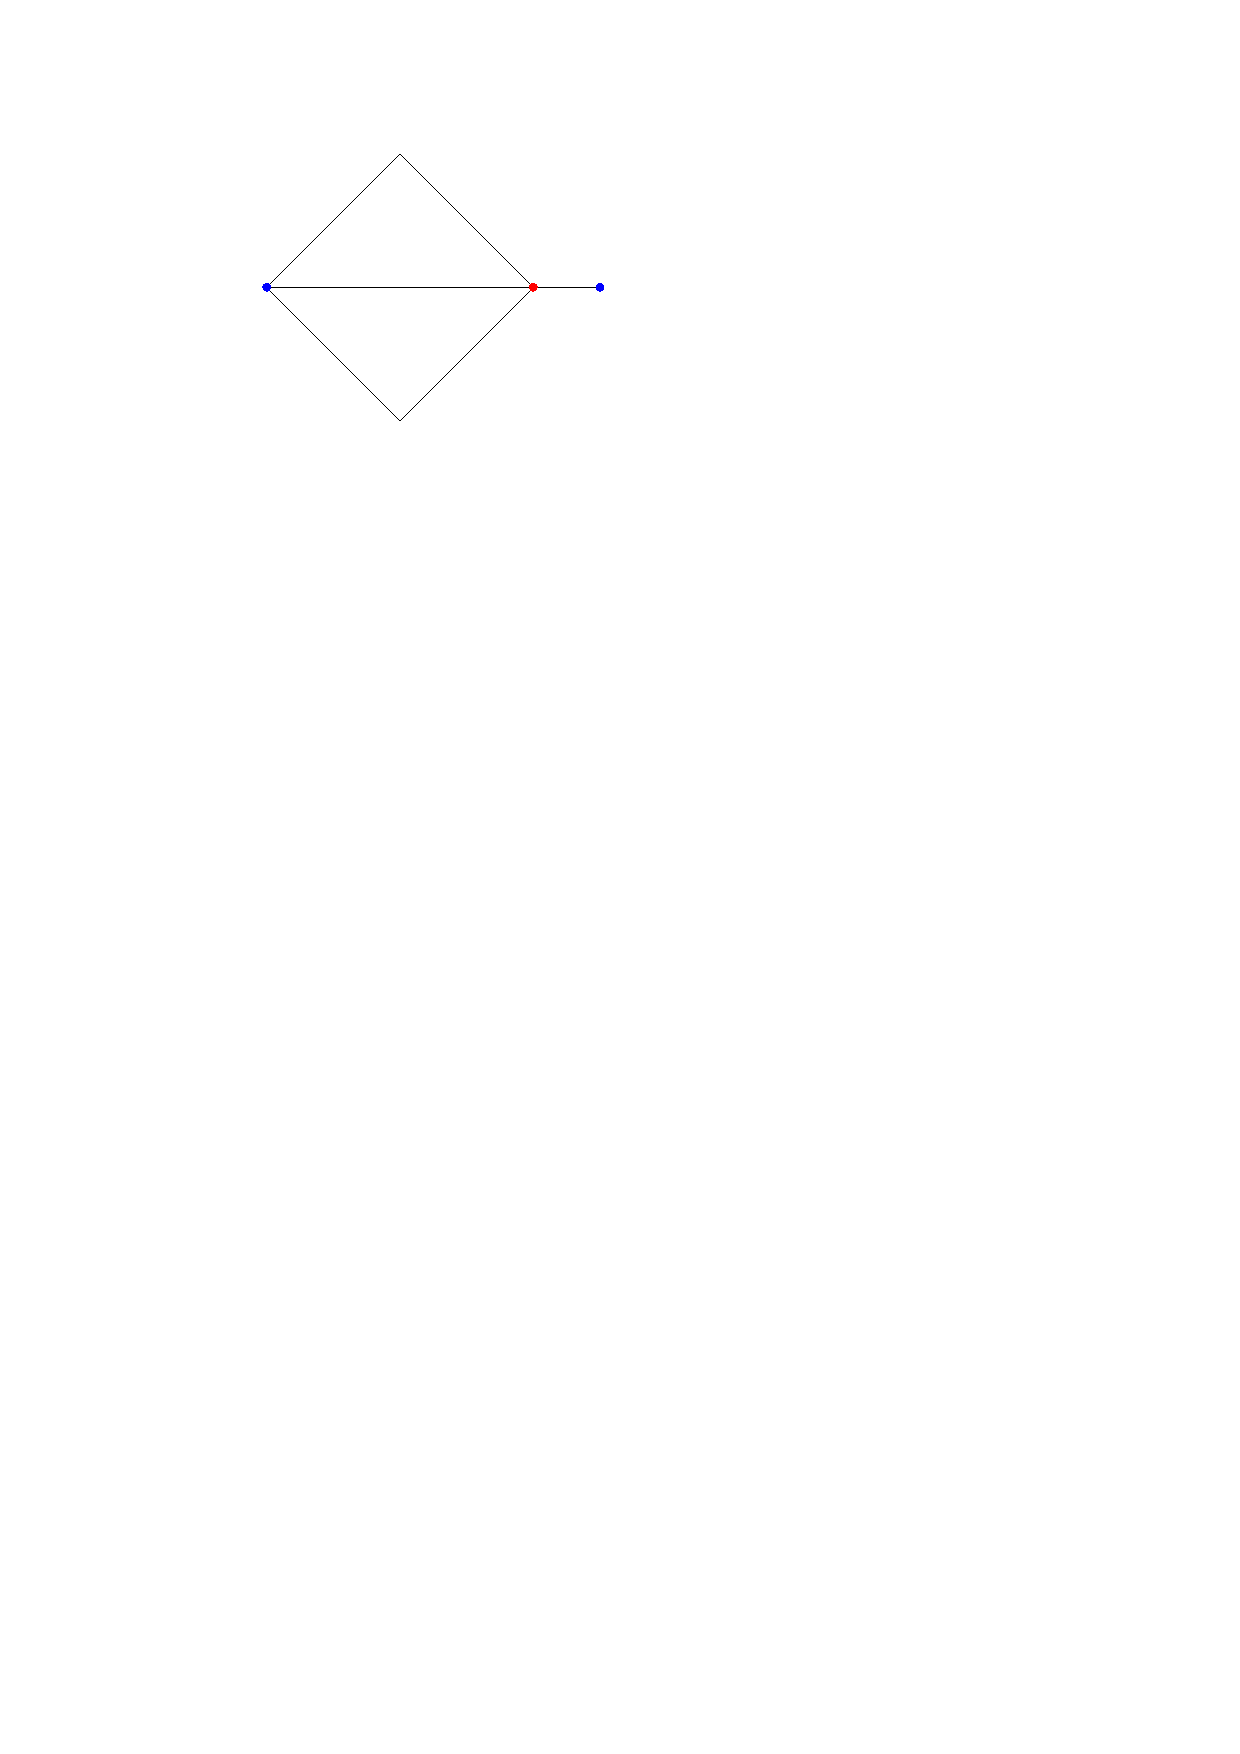
\includegraphics[width=20mm]{figures/crossFig10.pdf}} \\
      \small (f) &  (g) & (h) & (i) & (j) \\
      \hline
    \end{tabular}
    \caption{A collection of 10 different cases showing what we have 
             defined as an intersection between a polygon and a line segment}
	\label{fig:crossings}
\end{figure}

So given a polygon $O\in \mathcal{O}$, and a line segment $l$ we want to determine
weather $l$ crosses the polygon $O$. We start by making the list of points into
a list of line segment $O'=(p_1,p_2),(p_2,p_3),\dots,(p_{i-1},p_i)$.  Then we
observe that if a line segment crosses a line segment of a polygon, it counts
as a crossing (cases f and g). The other three cases of crossing (cases h, i
and j) all have that in common that the line segment crosses four end points
from the polygon. So we say it is not allowed to cross four points in of
a polygons line segments. The problem is that it makes (cases a, c
and d) illegal. But fortunately they all have that in common that they are collinear 
(they lie on a common line) with a line segment of the polygon, so the
algorithm is as follows:

\begin{enumerate}
	\item if a line segment $l_1$ crosses another line segment $l_2$ of a polygon it 
	      crosses the polygon
	\item if a line segment has four points in common with the polygon it crosses the
		  polygon, unless the line segment is collinear with a line segment of the
		  polygon 
\end{enumerate}

This lead us to the following algorithm
\nick{Write this algorithm}
\begin{algorithm} 
	\caption{NumberOfCrossings($l,P$)}
	\begin{algorithmic}[1] 
		\State \text{TODO}
	\end{algorithmic}
\end{algorithm}

\subsection{Crosses}
To make a crosses function, we need a right turn function. Consider three
points $p_1,p_2,p_3$ in the plane, make a line that goes through $p_1$ and $p_2$. 
Now if we stand at point $p_1$ and look in the direction of $p_2$ will $p_3$, if $p_3$
doesn't lie on the same line as $p_1$ and $p_2$ will it be on the
right or the left of the line. Let $p_i.x$ and $p_i.y$ denote the x-coordinates
and y-coordinates respectively. To find out whether the three points form a right turn, 
a left turn or are collinear we make the following two vectors.

\begin{align*}
	v_1 &=p_2-p_1 = \langle p_2.x-p_1.x,p_2.y-p_1.y\rangle\\
	v_2 &=p_3-p_1 = \langle p_3.x-p_1.x,p_3.y-p_1.y\rangle
\end{align*}
Lets denote $v_1 = \langle a,b\rangle$ and $v_2 = \langle c,d\rangle$
(see Figure \ref{fig:rightturn_a})

\subsection{Right turn}

\begin{figure}[H]
    \centering
	\begin{subfigure}{.7\textwidth}
		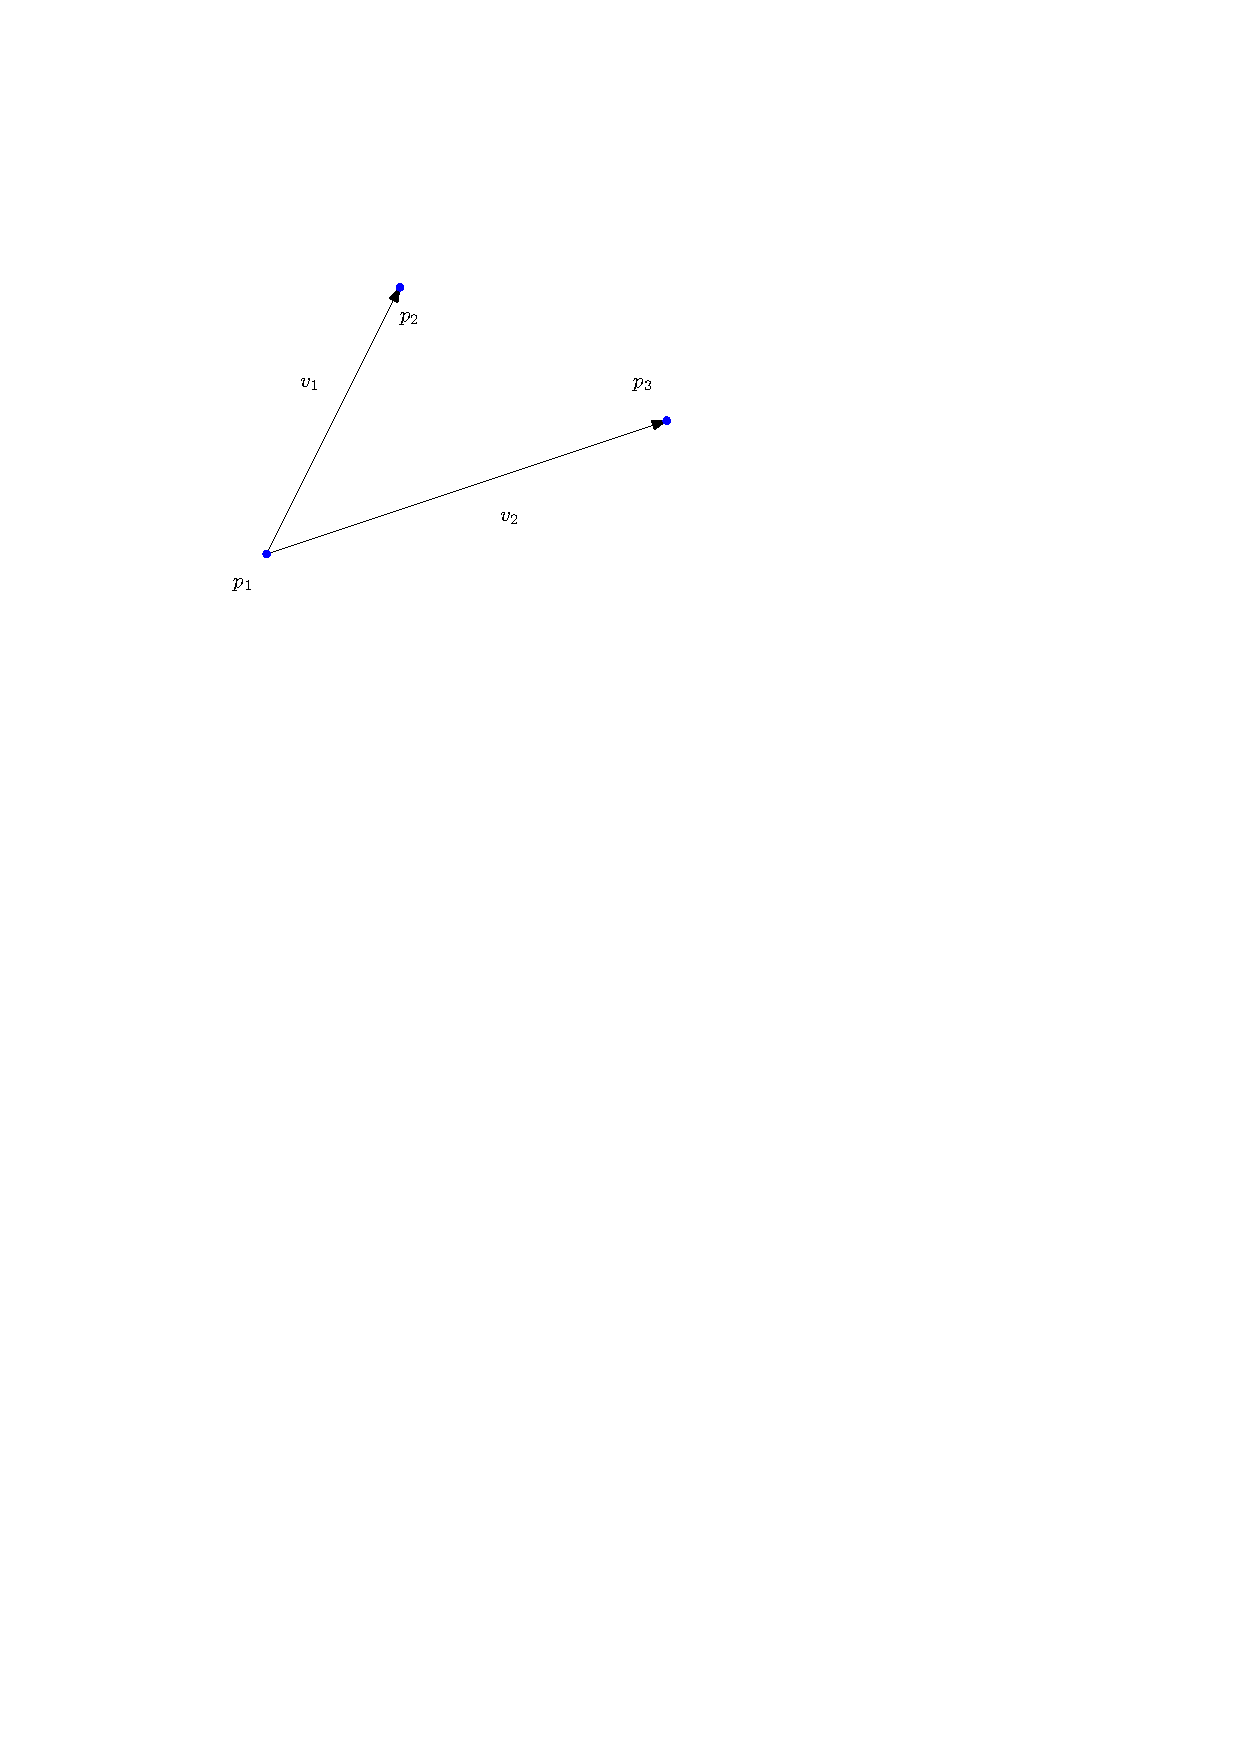
\includegraphics[width=8cm]{figures/rightturn1.pdf}
		\caption{}
		\label{fig:rightturn_a}
	\end{subfigure}
	\caption{A right turn formed by three points}
    %
	\begin{subfigure}{.7\textwidth}
		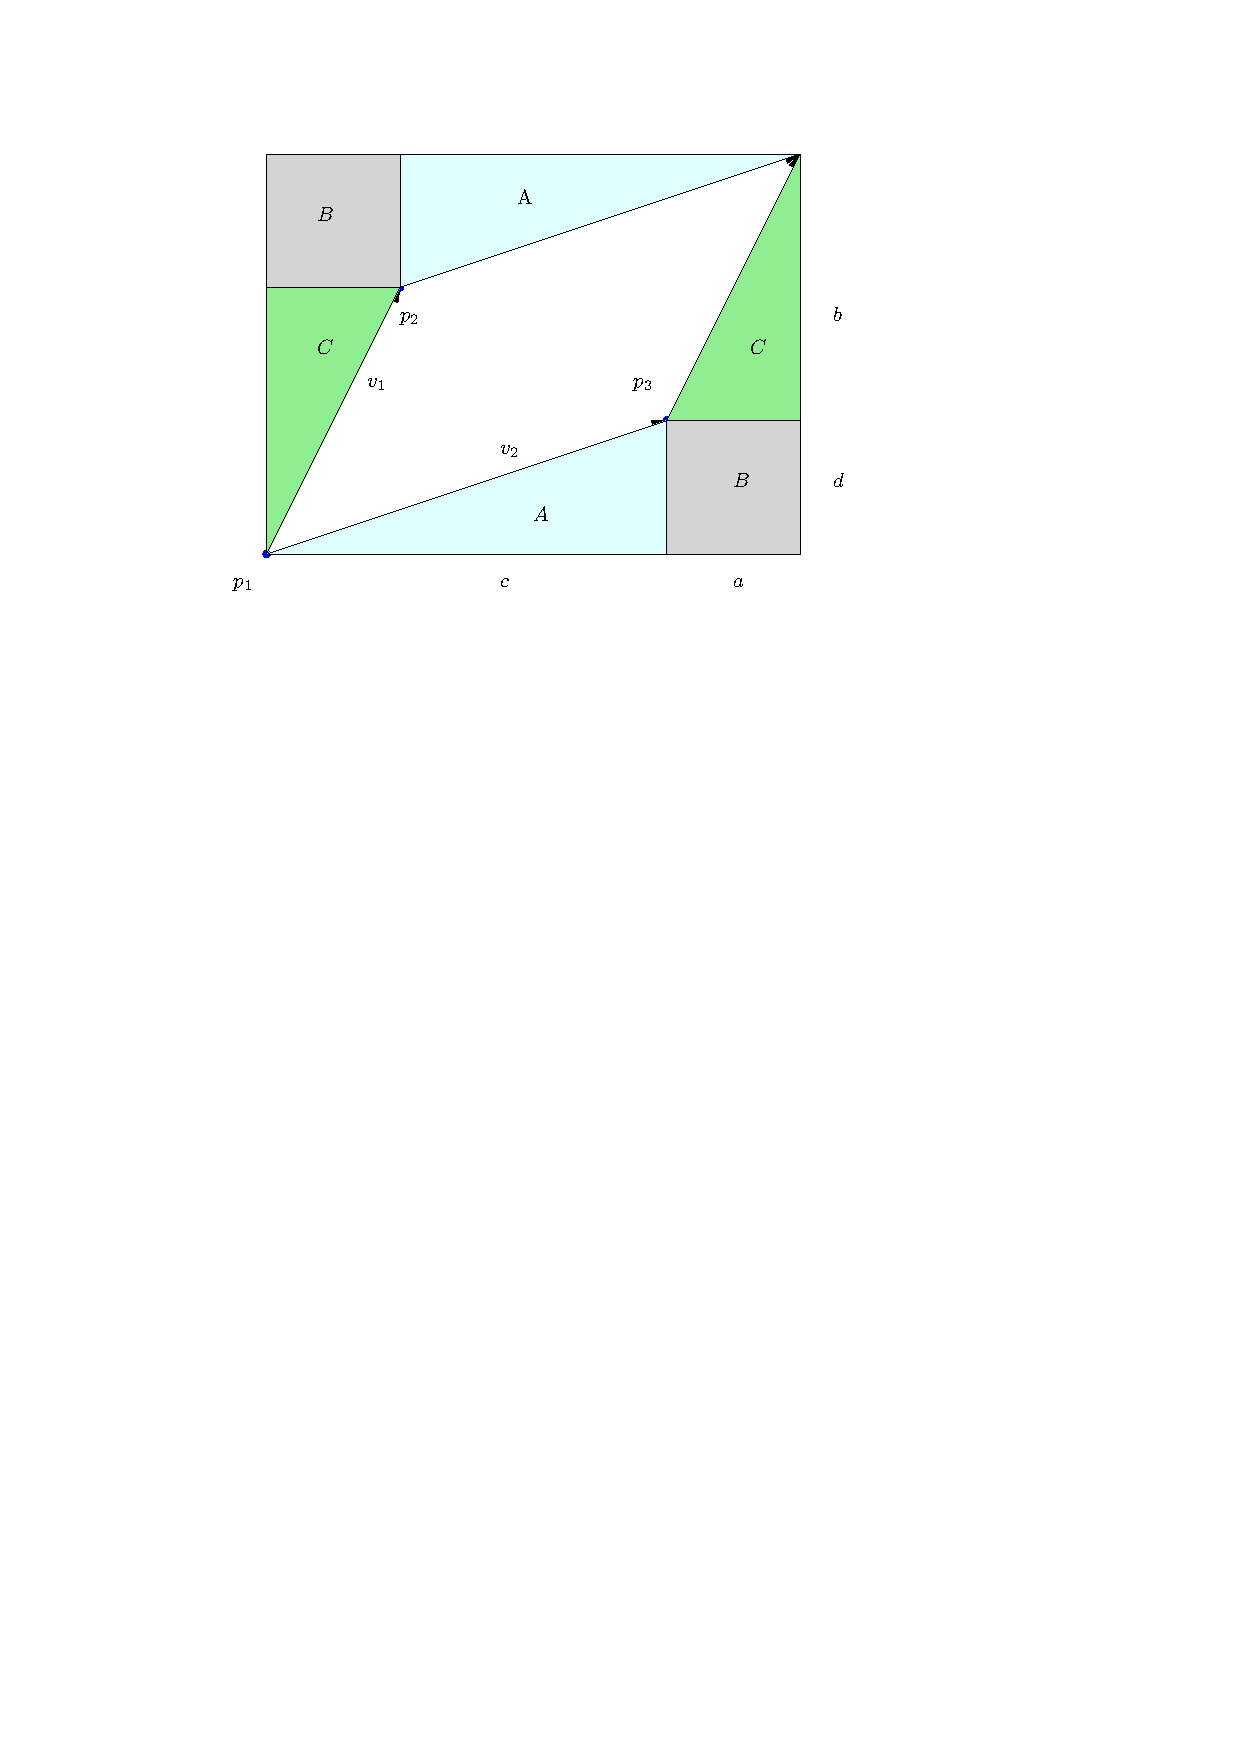
\includegraphics[width=8cm]{figures/rightturn2.pdf}
		\caption{}
		\label{fig:rightturn_b}
	\end{subfigure}
	\caption{Area are of a parallelogram given by two vectors}
\end{figure}

We claim that we can calculate the turn by calculating the signed area of the
parallelogram spanned by the two vectors. The area of their parallelogram can
be calculated as follows: calculate the area of the big rectangle, and take the
two small triangles and the little square and subtract that area.

\begin{align}
	\text{area} &= (a+c)(d+b)-2A-2B-2C\nonumber\\
							&=ad+ab+cd+bc-cd-2ad-ab\nonumber\\
							&=bc-ad \nonumber\\
							&=(p_2.y-p_1.y)(p_3.x-p_1.x)-(p_2.x-p_1.x)(p_3.y-p_1.y)\label{form:rightturn}
\end{align}

Now we claim that the area between these two vectors is positive if the
three points form a right turn, and negative if they form a left turn. We show
that by an example (see figure \ref{rightturn3})

Given our formula (formula \ref{form:rightturn}) we get that the $q_1,q_3,q_2$ area is

\begin{align*}
	&(q_3.y-q_1.y)(q_2.x-q_1.x)-(q_3.x-q_1.x)(q_2.y-q_1.y)\\ 
	= &(2-0)(-1-0)-(0-0)(1-0)\\
	= & 2\cdot (-1)-0\cdot1\\
	= & -2-0\\
	= & -2
\end{align*}
And the area of $q_1,q_3,q_4$ is
\begin{align*}
	&(q_3.y-q_1.y)(q_4.x-q_1.x)-(q_3.x-q_1.x)(q_4.y-q_1.y)\\ 
	= &(2-0)(1-0)-(0-0)(1-0)\\
	= &(2\cdot 1 - 0\cdot 1\\
	= &2-0\\
	= &2
\end{align*}

\begin{figure}[H]
    \centering
	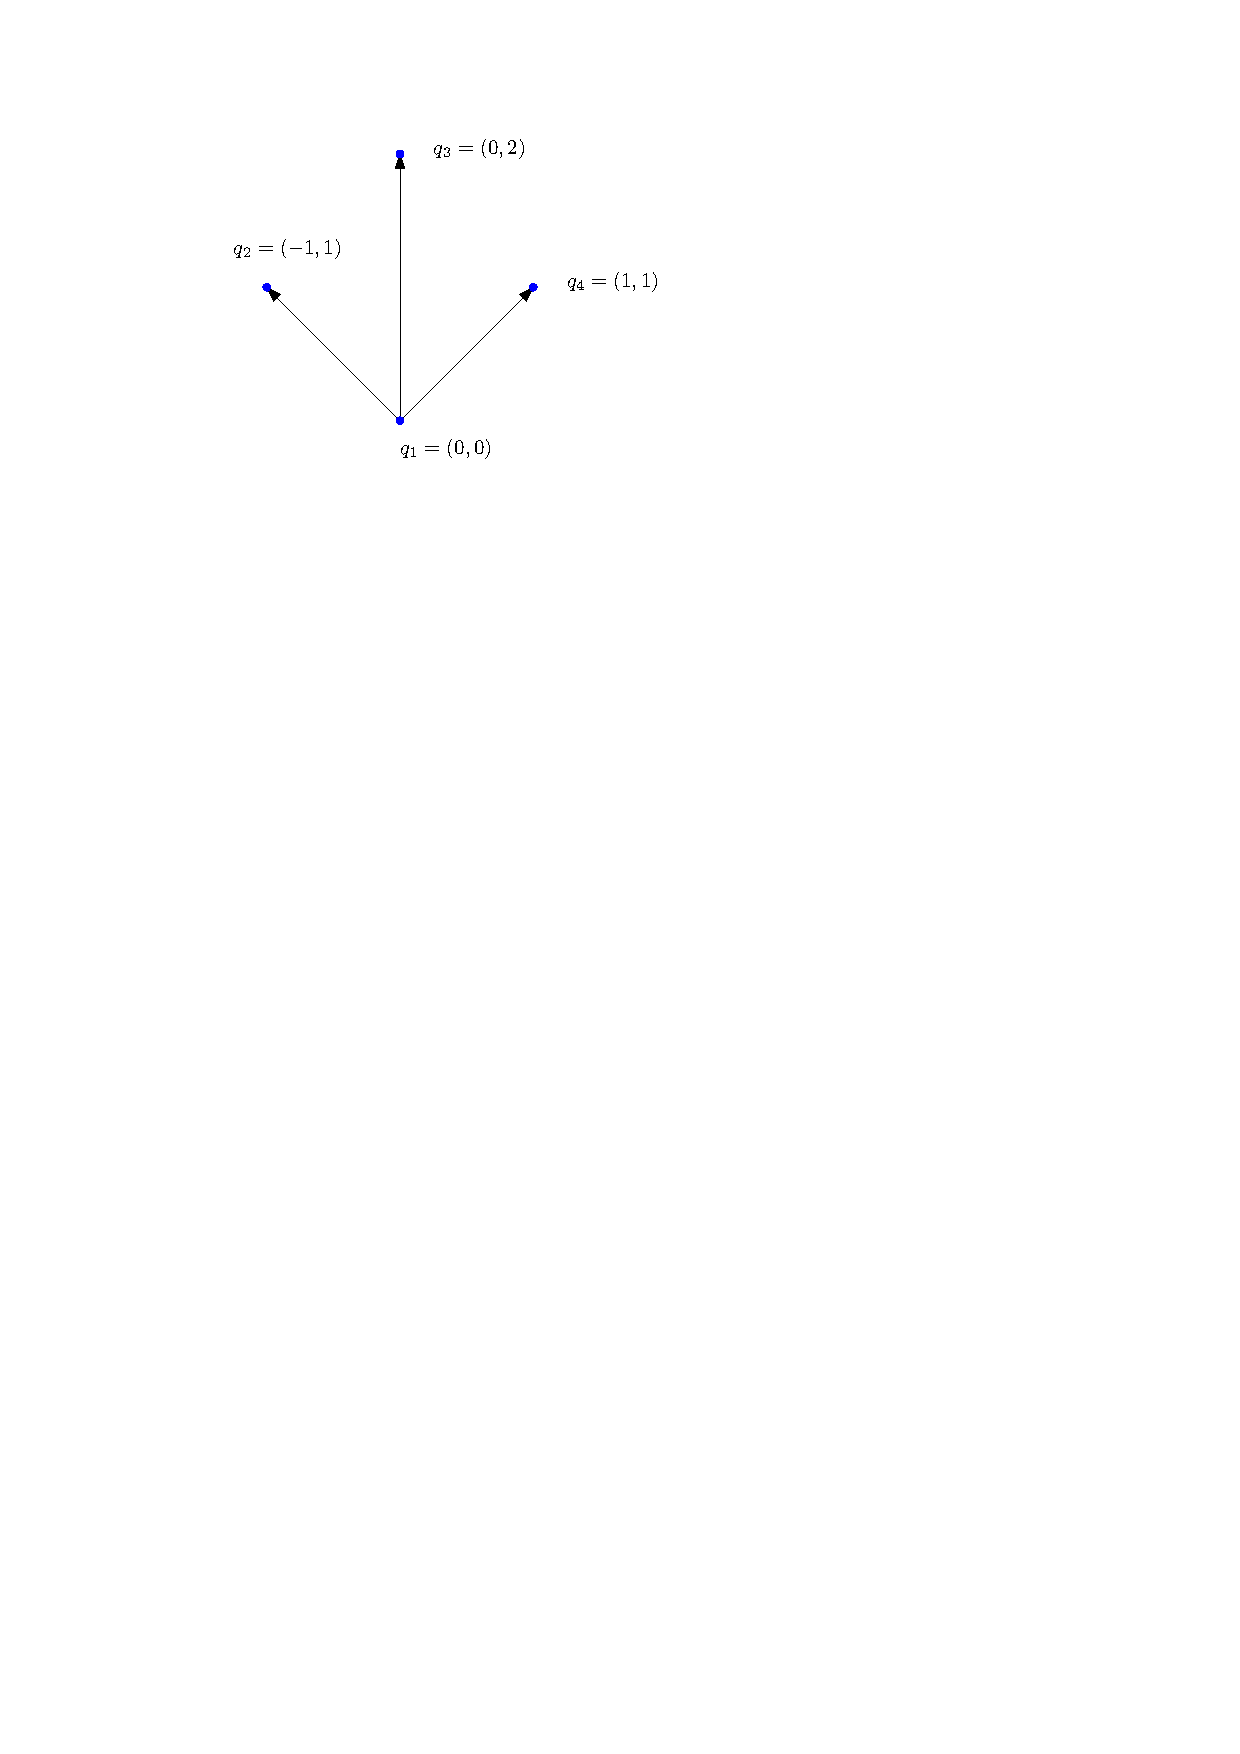
\includegraphics{figures/rightturn3.pdf}
	\caption{Right turn example}
    \label{rightturn3}
\end{figure}

So the function for calculating a right turn is

\begin{algorithm} 
	\begin{algorithmic}[1] 
		\State \Return $(p_2.x-p_1.x)(p_3.y-p_1.y)-(p_2.y-p_1.y)(p_3.x-p_1.x)$
	\end{algorithmic}
	\caption{rightTurn($p_1,p_2,p_3$)}
\end{algorithm}

This function will return a negative number if the three points make a left
turn, a positive number if it is a right turn and 0 if the three points are on
a line.

\subsection{Crossing of two line segments}

\begin{figure}[H]
	\minipage{0.32\textwidth}
		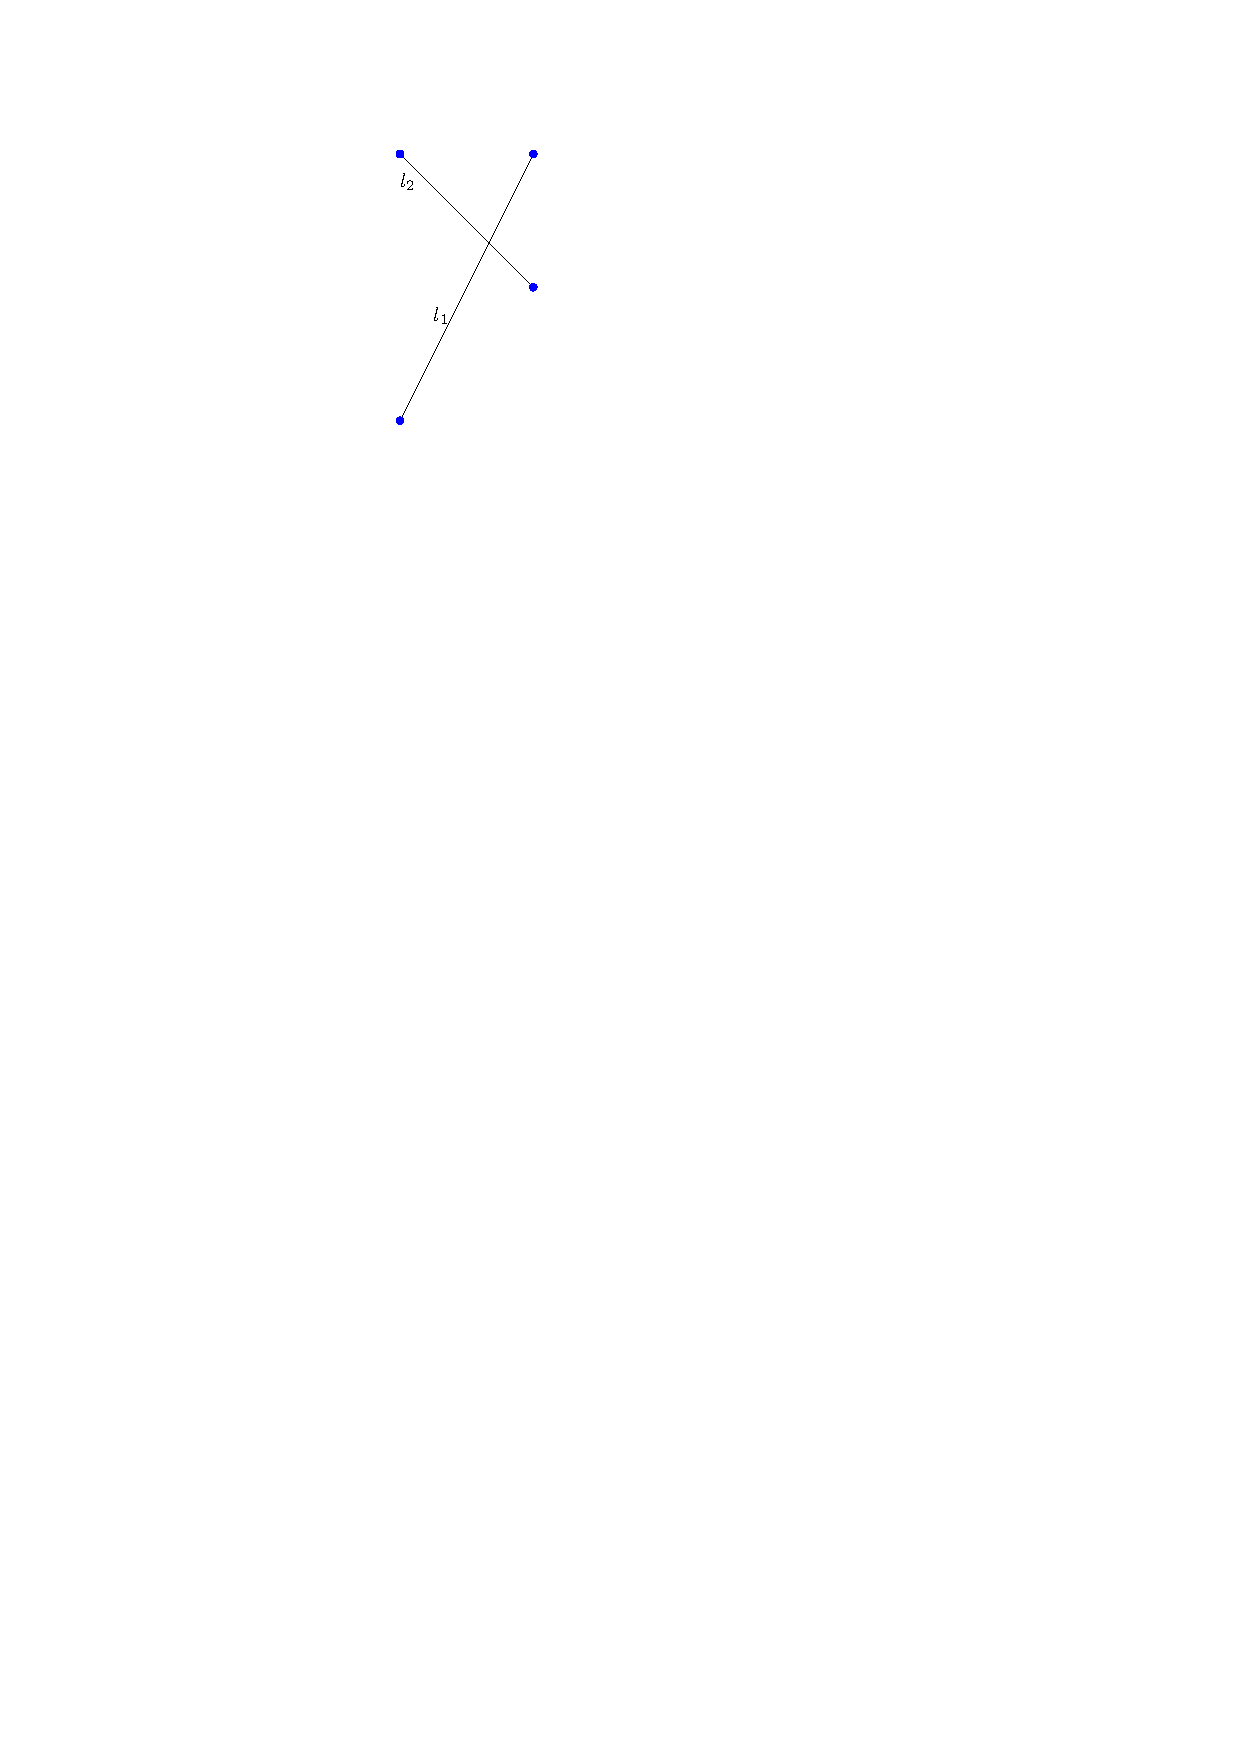
\includegraphics[width=2cm]{figures/crosses.pdf}
		\caption{Two lines crossing}
		\label{fig:crosses_a}
	\endminipage\hfill
	\minipage{0.32\textwidth}
		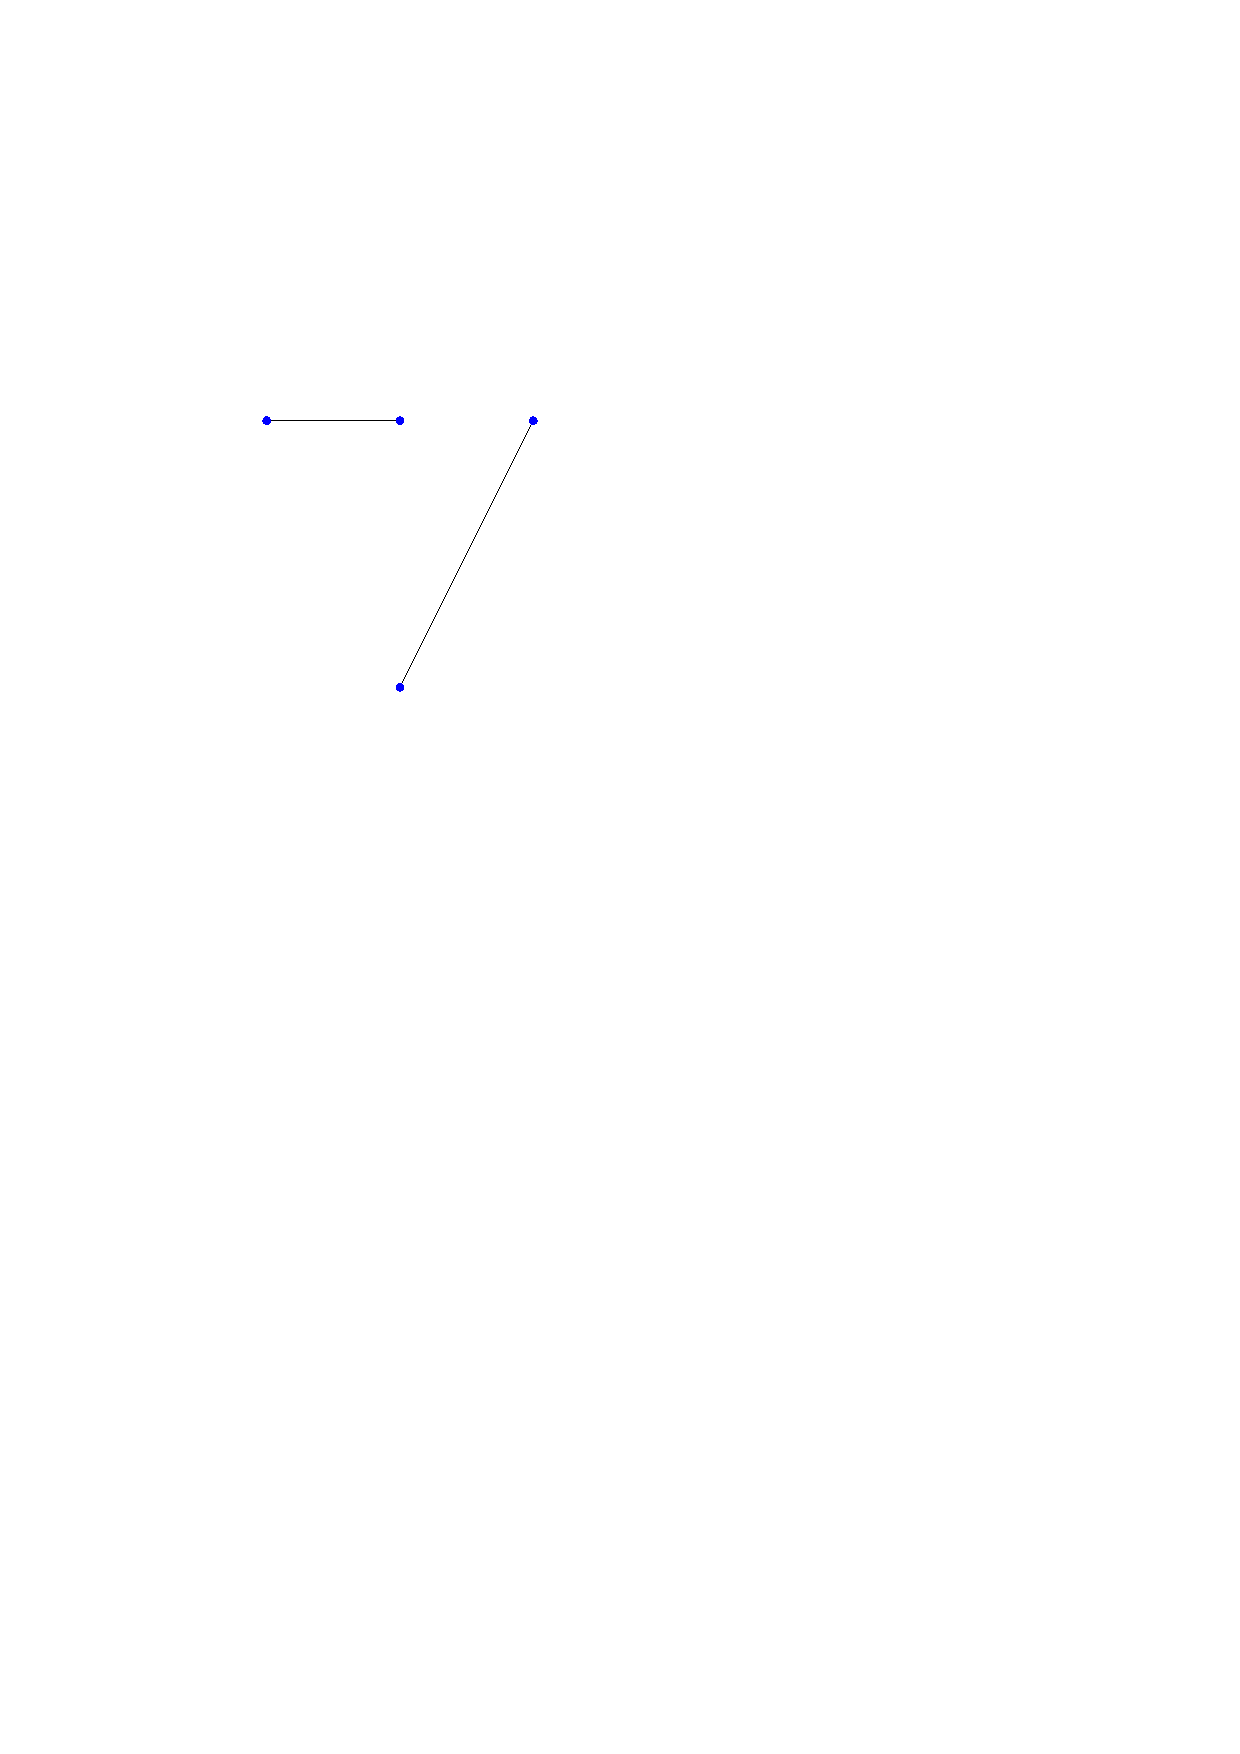
\includegraphics[width=3cm]{figures/crosses1.pdf}
		\caption{Two line which does not cross}
		\label{fig:crosses_b}
	\endminipage\hfill
	\minipage{0.32\textwidth}
		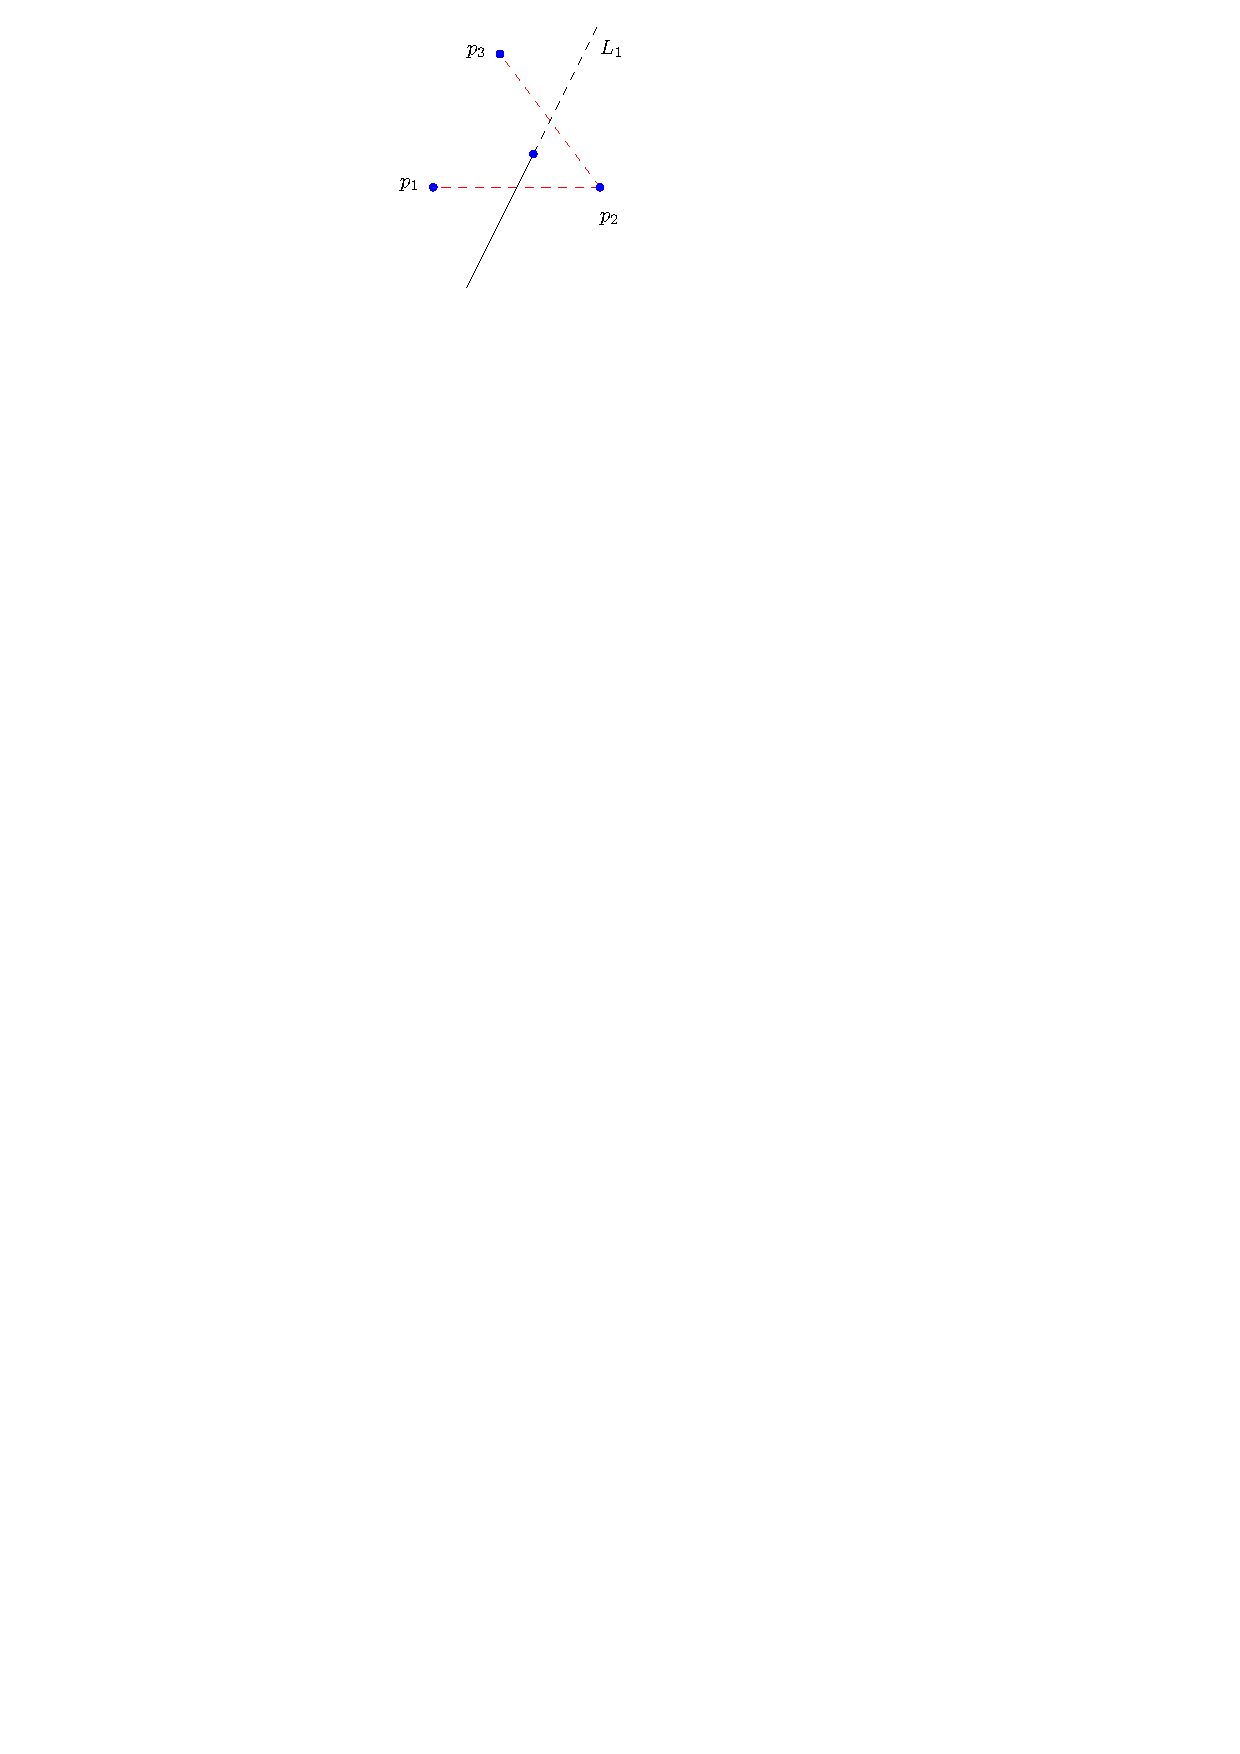
\includegraphics[width=3cm]{figures/crosses2.pdf}
		\caption{$\overline{p_1p_2}$ passes both tests of \ref{lemma:crosses}, while $\overline{p_2p_3}$ only passes one}
		\label{fig:crosses_c}
		\endminipage\hfill
\end{figure}

\begin{Lemma} \label{lemma:crosses}
    Given two line segments, $l_1$ and $l_2$ we can decide whether they cross
    by first checking if the two end points of $l_2$, namely $l_2.p$ and $l_2.q$, 
    lie on separate sides of the line which is collinear to $l_1$. Should this be
    the case, we do a similar check for $l_2$ on $l_1$. Should both cases be true
    we know $l_1$ crosses $l_2$, see figure \ref{fig:crosses_a}.
\end{Lemma}

\begin{proof}
Let $L_1$ and $L_2$ denote the lines collinear to $l_1$ and $l_2$ respectively.
	If both the end points of $l_2$ is on the same side of $L_1$, then the line
	segments can't cross $L_1$, and therefore $l_1$ obviously(see figure
	\ref{fig:crosses_b}). If they lie on opposite sites, $l_2$ crosses $L_1$ and
	we have to determine if $l_2$ crosses $L_1$ between $l_1.p$ and $l_1.q$. 

We know the line $l_2$ crosses $L_1$, the question is, is it between the two
	end points, we can quit easily determine this by looking at if the endpoints
	lie on opposite sites of $l_2$, like before(see figure \ref{fig:crosses_b}.
	If they do it must be the case that $l_1$ and $l_2$ crosses, if not it
	crosses $L_1$ another place.
\end{proof}

\subsection{Crosses algorithm}
We can check whether the endpoints of a line segment lie on opposite sites of another
line segment by multiplying the right turn results, since, if they lie on opposite sites,
they will have different sign, if they lie on the same side they have the same
sign so the result will be negative if they are on opposite sites and positive
if they are on the same side.
\nick{If its zero the hits an endpoint, write about that}
\begin{algorithm}[H]
	\caption{Crosses($l_1,l_2$)}
	\begin{algorithmic}[1] 
		\State foo = $rightTurn(l_1.p,l_1.q,l_2.p)\cdot
		rightTurn(l_1.p,l_1.q,l_2.q)$
		\State bar = $rightTurn(l_2.p,l_2.q,l_1.p)\cdot
		rightTurn(l_2.p,l_2.q,l_1.q)$
		\If{foo$<0$ and bar$<0$}
		\State \Return True
		\Else
		\State \Return False
		\EndIf
	\end{algorithmic}
\end{algorithm}

\section{Dijkstra}

the following description
is based on an "Introduction to Algorithms"\cite{IntroToAlg}, 24.3.

Dijkstra's algorithm solves the single-source shortest path problem for a
weighted directed graph $G$. i.e. Given a graph $G=(V,E)$, where $V$ is the
vertices and $E$ is the directed weighted edges and a start vertex $s\in V$,
find the path where the sum of the weights is the smallest possible.
Dijkstra original conceived the algorithm in his 1959 paper "A note on two
problems in connexion with graphs" \cite{dijkstra59}.

Let $v_\pi$ either be a predecessor of null. $v_d$ being the upper bound of
the weight of a shortest path from source $s$ to $v$. Running time $\Theta (V)$

\begin{algorithm} 
	\caption{Initialize-Single-Source(G,s)}
	\begin{algorithmic}[1] 
		\ForEach {vertex $v \in G.V$} 
			\State $v.d = \infty$
			\State $v.\pi =$ Null
		\EndFor 
		\State $s.d = 0$ 
	\end{algorithmic}
\end{algorithm}

Relaxing an edge $(u,v)$ consist of testing whether we can improve the shortest
path to $v$ found so far, by going through $u$ and, if so, update $v.d$ and
$v.\pi$. We define $w$ as following for a path $p=\langle v_0,v_1,...,v_k
\rangle$

$$ w(p) = \sum_{i=1}^k w(v_{i-1},v_i) $$

\begin{algorithm} 
	\caption{Relax(u,v,w)} 
	\begin{algorithmic}[1] 
		\If {$v.d > u.d + w(u,v)$} 
			\State $v.d=u.d+w(u,v)$ 
			\State $v.\pi = u$ 
		\EndIf 
		\State $s.d = 0$
	\end{algorithmic} 
\end{algorithm}

$Q$ acts as a min-priority queue to contain all the vertices in $V$. Naive
implementation of Dijkstra yields $O((V+E)lgV)$ which is $O(E \cdot lgV)$ if
all vertices are reachable from the source. And can be $O(V^2)$ if
$E=o(V^2/lgV)$. Extract min runs in $O(lgV)$ 

\begin{algorithm}[H]
	\caption{Dijkstra(G,w,s)} 
	\begin{algorithmic}[1] 
		\State Initialize-Single-Source(G,s) 
		\State $S = \emptyset$ 
		\State $Q = G.V$ 
		\While {$Q \not= \emptyset$} 
			\State $u = $Extract-Min(Q) 
			\State $S = S \cup \{u\}$
			\ForEach {vertex $v \in G.Adj[u]$} 
				\State Relax(u,v,w) 
			\EndFor 
		\EndWhile
	\end{algorithmic} 
\end{algorithm}

\section{Experiment}
In this section we present the experiments we did on our $O(n^3+kn^2)$ implementation,
both for running time and test of correctness.

\subsection{Computer specification}
The test were run on a computer with the following specification
\begin{figure}[H]
\begin{tabular}{| c | l |}
	\hline
	Model & Lenovo ThinkPad, x230 \\
	\hline
	Operating system & Arch Linux \\
	\hline
	CPU & Intel(R) Core(TM) i7-3520M CPU @ 2.90GHz\\
	\hline
	Memory & 8 GB \\
	\hline
\end{tabular}
\end{figure}

\subsection{Correctness of algorithm}
To verify the correctness of our implementation we run the code against a list of tests.
We implemented the function to output a svg image of the polygons and route so we
were able to confirm the algorithm made the correct visibility graph. (See
figure \ref{fig:correctness_1} and \ref{fig:correctness_2}
\begin{figure}[H]
	\begin{subfigure}{.5\textwidth}
		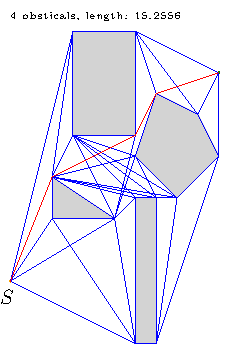
\includegraphics[width=6cm]{figures/correctness1.pdf}
		\caption{}
		\label{fig:correctness_1}
	\end{subfigure}
	\begin{subfigure}{.5\textwidth}
		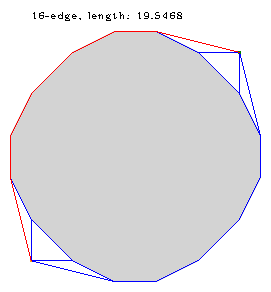
\includegraphics[width=6cm]{figures/correctness2.pdf}
		\caption{}
		\label{fig:correctness_2}
	\end{subfigure}
	\caption{Examples of figures for correctness}
\end{figure}

\subsection{Running time of algorithm}
To test the running time of our implementation we auto generated a map consisting of
x times x squares and put $s$ and $t$ in opposite corners of the map (see figure
\ref{fig:test})

\begin{figure}[H]
    \centering
	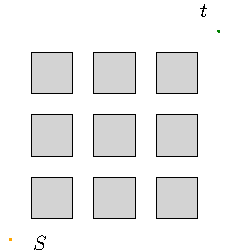
\includegraphics[width=6cm]{figures/testexample.pdf}
	\label{fig:test}
	\caption{Examples of figures for correctness}
\end{figure}
\label{testfilegeneration}
We ran the implementation with the number of violations being constant at $5$ and the
number of vertices was $n= 4 \cdot t^2$ for $t=1,\dots,41$ and got the following graph

\begin{center}
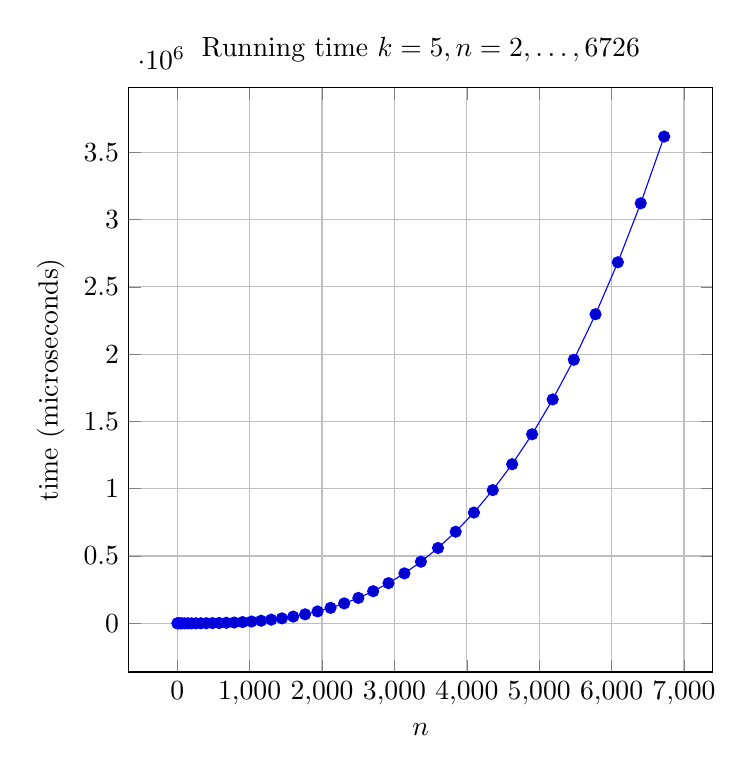
\begin{tikzpicture}
\begin{axis}[
		%xmode=log,
title={Running time $k=5,n=2,\dots,6726$},
height=9cm,
width=9cm,
grid=major,
xlabel = $n$,
ylabel = time (microseconds),
]
\addplot coordinates {
	(2,0)
	(6,0)
	(18,0)
	(38,1)
	(66,9)
	(102,24)
	(146,50)
	(198,112)
	(258,235)
	(326,466)
	(402,848)
	(486,1481)
	(578,2462)
	(678,3939)
	(786,6083)
	(902,9271)
	(1026,13357)
	(1158,19278)
	(1298,27520)
	(1446,37018)
	(1602,50129)
	(1766,66930)
	(1938,88378)
	(2118,114971)
	(2306,148055)
	(2502,188859)
	(2706,238534)
	(2918,298675)
	(3138,371052)
	(3366,457771)
	(3602,559747)
	(3846,680632)
	(4098,822848)
	(4358,989762)
	(4626,1182116)
	(4902,1404667)
	(5186,1663503)
	(5478,1958169)
	(5778,2296425)
	(6086,2682430)
	(6402,3120744)
	(6726,3616376)
};
\end{axis}
\end{tikzpicture}

\end{center}

Then we tried figuring out where the time was spent so we tried measuring the
crossing function, the construction of visibility graph and the Dijkstra
separately and got the following

\begin{center}
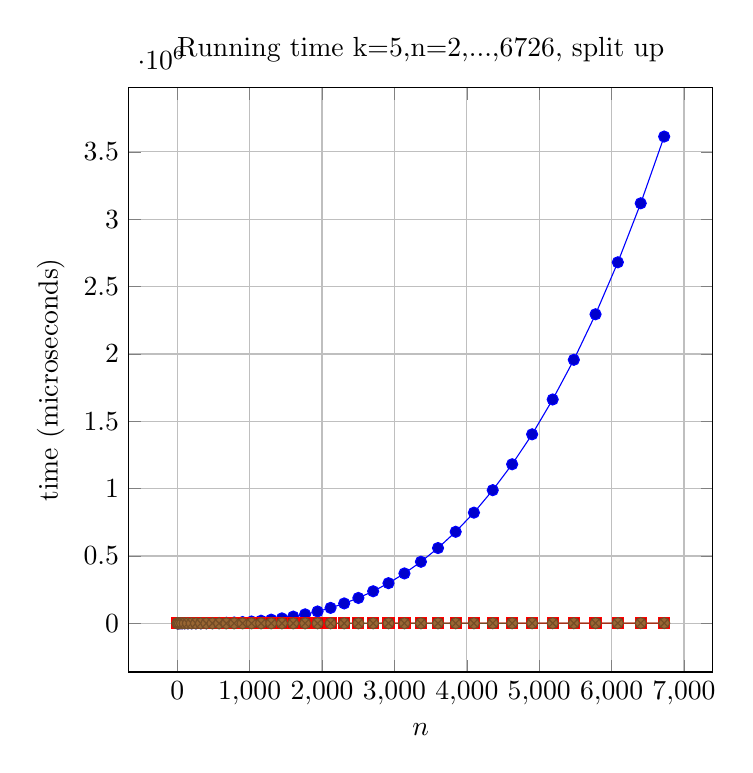
\begin{tikzpicture}
\begin{axis}[
title={Running time k=5,n=2,...,6726, split up},
height=9cm,
width=9cm,
grid=major,
xlabel = $n$,
ylabel = time (microseconds),
]
\addplot coordinates {
%crossing
	(2,0)
	(6,0)
	(18,0)
	(38,1)
	(66,8)
	(102,22)
	(146,45)
	(198,104)
	(258,222)
	(326,447)
	(402,821)
	(486,1444)
	(578,2415)
	(678,3878)
	(786,6006)
	(902,9178)
	(1026,13244)
	(1158,19144)
	(1298,27359)
	(1446,36821)
	(1602,49895)
	(1766,66658)
	(1938,88071)
	(2118,114616)
	(2306,147650)
	(2502,188395)
	(2706,237995)
	(2918,298074)
	(3138,370383)
	(3366,457025)
	(3602,558914)
	(3846,679704)
	(4098,821822)
	(4358,988634)
	(4626,1180886)
	(4902,1403311)
	(5186,1662007)
	(5478,1956547)
	(5778,2294661)
	(6086,2680522)
	(6402,3118674)
	(6726,3614138)
};
\addplot coordinates {
%visibility 
	(2,0)
	(6,0)
	(18,0)
	(38,0)
	(66,0)
	(102,0)
(146,1)
(198,2)
(258,3)
(326,4)
(402,6)
(486,9)
(578,11)
(678,15)
(786,18)
(902,22)
(1026,28)
(1158,33)
(1298,40)
(1446,47)
(1602,56)
(1766,65)
(1938,75)
(2118,87)
(2306,100)
(2502,115)
(2706,131)
(2918,148)
(3138,167)
(3366,190)
(3602,213)
(3846,238)
(4098,264)
(4358,298)
(4626,328)
(4902,363)
(5186,400)
(5478,440)
(5778,481)
(6086,530)
(6402,574)
(6726,628)
};
\addplot coordinates {
%Dijkstra
	(2,0)
(6,0)
(18,0)
(38,0)
(66,1)
(102,2)
(146,4)
(198,6)
(258,10)
(326,15)
(402,21)
(486,28)
(578,36)
(678,46)
(786,59)
(902,71)
(1026,85)
(1158,101)
(1298,121)
(1446,150)
(1602,178)
(1766,207)
(1938,232)
(2118,268)
(2306,305)
(2502,349)
(2706,408)
(2918,453)
(3138,502)
(3366,556)
(3602,620)
(3846,690)
(4098,762)
(4358,830)
(4626,902)
(4902,993)
(5186,1096)
(5478,1182)
(5778,1283)
(6086,1378)
(6402,1496)
(6726,1610)
};
\end{axis}
\end{tikzpicture}

\end{center}

The implementation is totally dominated by the crossing calculating which makes
sense since the $O(n^3)$ is the most dominant sub time, we tried dividing the first graph
with $O(n^3)$ and got the following

\begin{center}
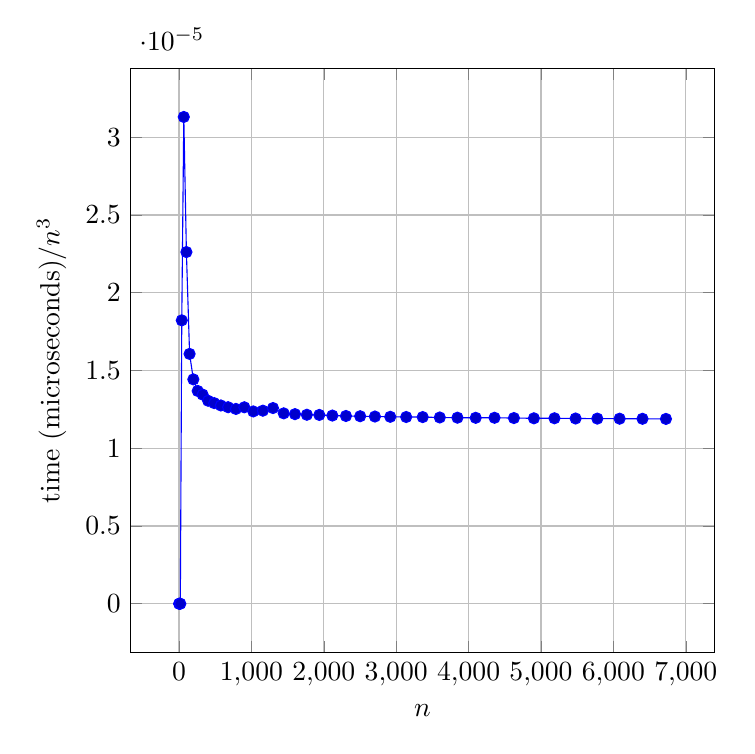
\begin{tikzpicture}
\begin{axis}[
height=9cm,
width=9cm,
grid=major,
xlabel = $n$,
ylabel = time (microseconds)/$n^3$,
]
\addplot coordinates {
	(2,0)
	(6,0)
	(18,0)
	(38,1.82242309374544E-05)
	(66,3.13047833708991E-05)
	(102,2.26157360291291E-05)
	(146,1.60661359272217E-05)
	(198,1.44285421297971E-05)
	(258,1.36838638480003E-05)
	(326,1.34503354733029E-05)
	(402,1.3053221060855E-05)
	(486,1.29016795495295E-05)
	(578,1.27498340864401E-05)
	(678,1.26385397648696E-05)
	(786,1.25270894447943E-05)
	(902,1.26330137388433E-05)
	(1026,1.2367070702209E-05)
	(1158,1.24147019560424E-05)
	(1298,1.25841634982224E-05)
	(1446,1.2243570102851E-05)
	(1602,1.21927454179994E-05)
	(1766,1.2152027041557E-05)
	(1938,1.21417937429069E-05)
	(2118,1.21006985351175E-05)
	(2306,1.20738331437455E-05)
	(2502,1.20580136097767E-05)
	(2706,1.20383485707373E-05)
	(2918,1.20210667777948E-05)
	(3138,1.20081459851104E-05)
	(3366,1.20034459584254E-05)
	(3602,1.19773474781993E-05)
	(3846,1.19642236814143E-05)
	(4098,1.19564913967957E-05)
	(4358,1.19582904652676E-05)
	(4626,1.19410690659842E-05)
	(4902,1.19248646628465E-05)
	(5186,1.19268580687987E-05)
	(5478,1.19119836093996E-05)
	(5778,1.19047328401354E-05)
	(6086,1.1899605218836E-05)
	(6402,1.18935399250374E-05)
	(6726,1.18851040850164E-05)
};
\end{axis}
\end{tikzpicture}

\end{center}

Lastly we tried to make a test where $n=25^2$ and $k=1,\dots,25$ and getting
the almost linear graph

\begin{center}
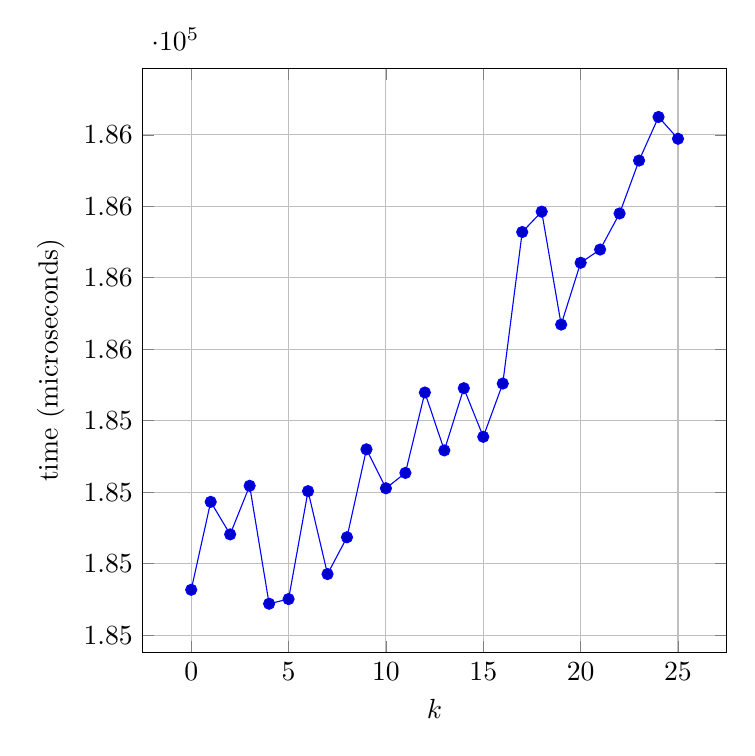
\begin{tikzpicture}
\begin{axis}[
height=9cm,
width=9cm,
grid=major,
xlabel = $k$,
ylabel = time (microseconds),
]

\addplot coordinates {
	(0,184927)
	(1,185173)
	(2,185082)
	(3,185218)
	(4,184888)
	(5,184901)
	(6,185203)
	(7,184971)
	(8,185074)
	(9,185320)
	(10,185211)
	(11,185254)
	(12,185479)
	(13,185317)
	(14,185491)
	(15,185355)
	(16,185504)
	(17,185928)
	(18,185985)
	(19,185669)
	(20,185842)
	(21,185879)
	(22,185980)
	(23,186128)
	(24,186250)
	(25,186189)
};
\end{axis}
\end{tikzpicture}

\end{center}

In conclusion we have implemented a naive $O(n^3 + kn^2)$ algorithm and made tests both
for confirming its correctness and its running time of the algorithm.


\chapter{Continuous Dijkstra - overview of $O(k^2 n \log n)$ algorithm}

The following chapter is dedicated to giving the reader an overview of an $O(k^2 n \log n)$ 
time algorithm for solving the shortest path with obstacle violation. First we present an 
overview of the Hershberger-Suri algorithm, which solves the shortest path with no violation, 
in an optimal $O(n \log n)$ time \cite{HershbergerS99}. This algorithm produces a shortest 
path map, which divides the free space, free space being the plane minus the interior of the 
obstacles, into subdivision where each subdivision will have the same shortest sub-path to 
all points in the area. This structure can then be extended for the purpose of calculating 
shortest paths with violation, which we will present an intuitive idea on how this is done. 
Finally we present an algorithm which will combine the Hershberger-Suri algorithm with a 
modified version of the same algorithm, to produce a shortest $k$-path map, a subdivision 
which has the shortest sub-path to all points in an area with $k$ violations, in time $O(k^2 
n \log n)$. This result is due to Hershberger, Kumar and Suri \cite{HershbergerKS17}.

\section{The Hershberger-Suri algorithm overview}

The Hershberger-Suri algorithm is an algorithm for computing the shortest 
path in a plane in the presence of obstacles without violations. The 
Hershberger-Suri algorithm was proven to be optimal-time in \cite{HershbergerS99}, 
with its $O(n \log n)$ running time, with $n$ being the total number of vertices 
of the obstacles located in the plane. This is done by computing a shortest path map 
which is  a map containing the shortest paths from a fixed source point $s$, to all 
other points in the plane. This is done by subdividing the plane into a finite number
of regions, where all the points in such a region have the same shortest sub-path
from $s$. This map can be constructed in $O(n\log n)$ time and requires $O(n\log n)$ 
space A query for a shortest path can be processed in $O(\log n)$
time.

The first step in the Hershberger-Suri algorithm is to use an implementation of
the continuous Dijkstra method, which purpose is to give a distance from the
source $s$ to each vertex and edge in the plane. The continuous Dijkstra method
is a theoretical tool to simulate a propagation of a unit speed wavefront in a
free space, where $s$ sends out the first emission, which propagates through
the plane and collides with obstacles. Upon collision between a wavefront and
a vertex in an obstacle, then this vertex will also start emitting a wavefront
of its own, with its weight equal to the time it took from $s$ started to emit
its wavefront until a contact (with any wavefront). 

Hershberger and Suri introduced two new ideas to speed the implementation of the
continuous Dijkstra method up compared to previous attempts, the first being a 
quad-tree-like subdivision of the plane, which we'll later introduce as a conforming 
subdivision, and the second being an approximate wavefront, which introduces a
bit of slack in the calculation of the collision-time of the wavefronts.

The first idea is grounded in the observation that a wavefront of the type in the 
continuous Dijkstra method, will be quite complicated to implement directly. 
A subdivision of the plane into well-behaved regions will be a way around this. 
This subdivision is constructed in such a way that it aids the propagation of the 
wavefronts. This is done by temporarily ignoring the line segments(edges) between the 
vertices in the obstacles, and subdividing the plane into a grid-like subdivision of 
size $O(n)$ around the vertices. Each cell in this subdivision, (the conforming 
subdivision) will only have a constant number of straight line edges, and will contain 
at most one obstacle vertex. This construction means that the subdivision satisfies the 
following crucial property: for any edge $e$ of the subdivision, there are $O(1)$ cells 
within distance $2|e|$ of $e$, which will be crucial in bounding the overall complexity
of the subdivision.

The obstacle line segments will then be inserted into the subdivision, while
maintaining both the linear size of the subdivision and its conforming property, except 
now a non-obstacle edge $e$ will have the property of having $O(1)$ cells within 
shortest path distance $2|e|$ of the edge.

These cells will then form the basis for the \textit{unitspeed} propagation in the 
algorithm, which will act as the wavefront propagation in the algorithm. This means 
that at each step the wavefront will propagated through one cell at a time for each 
time count. Since the descriptive complexity of each cell will be constant the 
algorithm will perform efficiently in the propagation through of the cells.

Inside each of these cells there will be two types of event: the first being a
collision between a wavefront and an obstacle, which is quite easy to handle. The 
second type of event will be a collisions between two wavefronts which will be more 
complex problem to handle. There will be two different types of collisions between two 
wavefronts, the first being the collisions where the wavelets are neighbors in the 
wavefront, and the second being collisions between non-neighboring wavelets. Here two 
wavefronts are waves emitted from two different sources, and two wavelets being two 
parts of the wave arch emitted from one source. The case of colliding neighboring 
wavelets occurs when a wavelet would be engulfed by the expansion of wavelets of its 
two neighbors and should be quite easy to detect and process. The collision between 
non-neighboring wavelets, however are more troublesome, and to process these we make 
use of the second idea: approximate wavefront.

The idea of approximating wavefronts is the abandonment of trying to compute the exact 
time of collision and instead maintaining two separate wavefronts approaching the edge 
from opposite sides. Each of these wavefronts is an \textit{approximate wavefront}, 
representing the wavefront that hits the edge from only one side. This leads to the 
other wavefronts which arrives at the edge after first wavefront, wont be recorded by 
the edge, due to it being slower than the initial arriving wavefront.

As mentioned above the Hershberger-Suri algorithm make use of timers to estimate the 
distance between two points in the plane but also to estimate when each edge in the 
subdivision would be engulfed by the wavefronts. A critical task of these timers is to 
ensure that the collision between two wavefronts which are used in the construction of 
the shortest path map, is measured in a small proximity of their actual collision, and 
therefore location.

At the end of the propagation phase, all the collision information is collected, and 
then a Voronoi diagram like technique is used in each cell to compute the collision 
events in that cell precisely. These collisions determines the edges of the final 
shortest path map, which will give us the shortest path to every point in the plane.

\section{From no violations to k-violations}

Previously, we've given an overview of the Hershberger-Suri algorithm which calculates a 
shortest path map ($SPM$) in $O(n\log n)$ time from a source point $s$ 
\cite{HershbergerS99}. By modifying the algorithm, and using it in as a subroutine 
Hershberger, Kumar and Suri showed an algorithm for calculating the shortest path map, 
where every route would violated at most $k$ obstacles from $s$ to an endpoint 
$t$\cite{HershbergerKS17}. This  is done by calculating a shortest $k$-path map, which in 
essence would produce a subdivision of the plane into regions, as done by the 
Hershberger-Suri algorithm, but with the guarantee of every path violating at most $k$ 
obstacles. A way to better understand how such a map would be calculated is by using the 
metaphor of a parking garage. Here every obstacle would be seen as an elevator from one 
floor $i$ to the next floor $i+1$. This would imply one could only take at most $k$ 
elevator trips when taking the path from $s$ to $t$. When thinking about the problem in 
this way, it seems quite natural to think of the construction of $SPM_k$ iteratively, 
starting by making the $SPM_0$ map, which is done by the Hershberger-Suri algorithm, and 
then from this construct the $SPM_1$ map, and for each iteration going one floor up, 
until we reach $SPM_{k-1}$.

\section{Construction of a shortest $k$-path map}

The $O(k^2 n \log n)$ implementation of shortest path with obstacle violation, makes use 
both of a unchanged and a modification version of the Hershberger-Suri algorithm. The 
unchanged version is used to prepare the $SPM_0$ map, which the modified version then 
uses to iteratively calculate the $SPM_k$ map. The change is due to the unchanged 
algorithm starts the wave propagation from a source point $s$ which propagates through 
the plane. 

\begin{figure}[H]
\centering
\caption{}
\begin{subfigure}{.5\textwidth}
  \centering 
  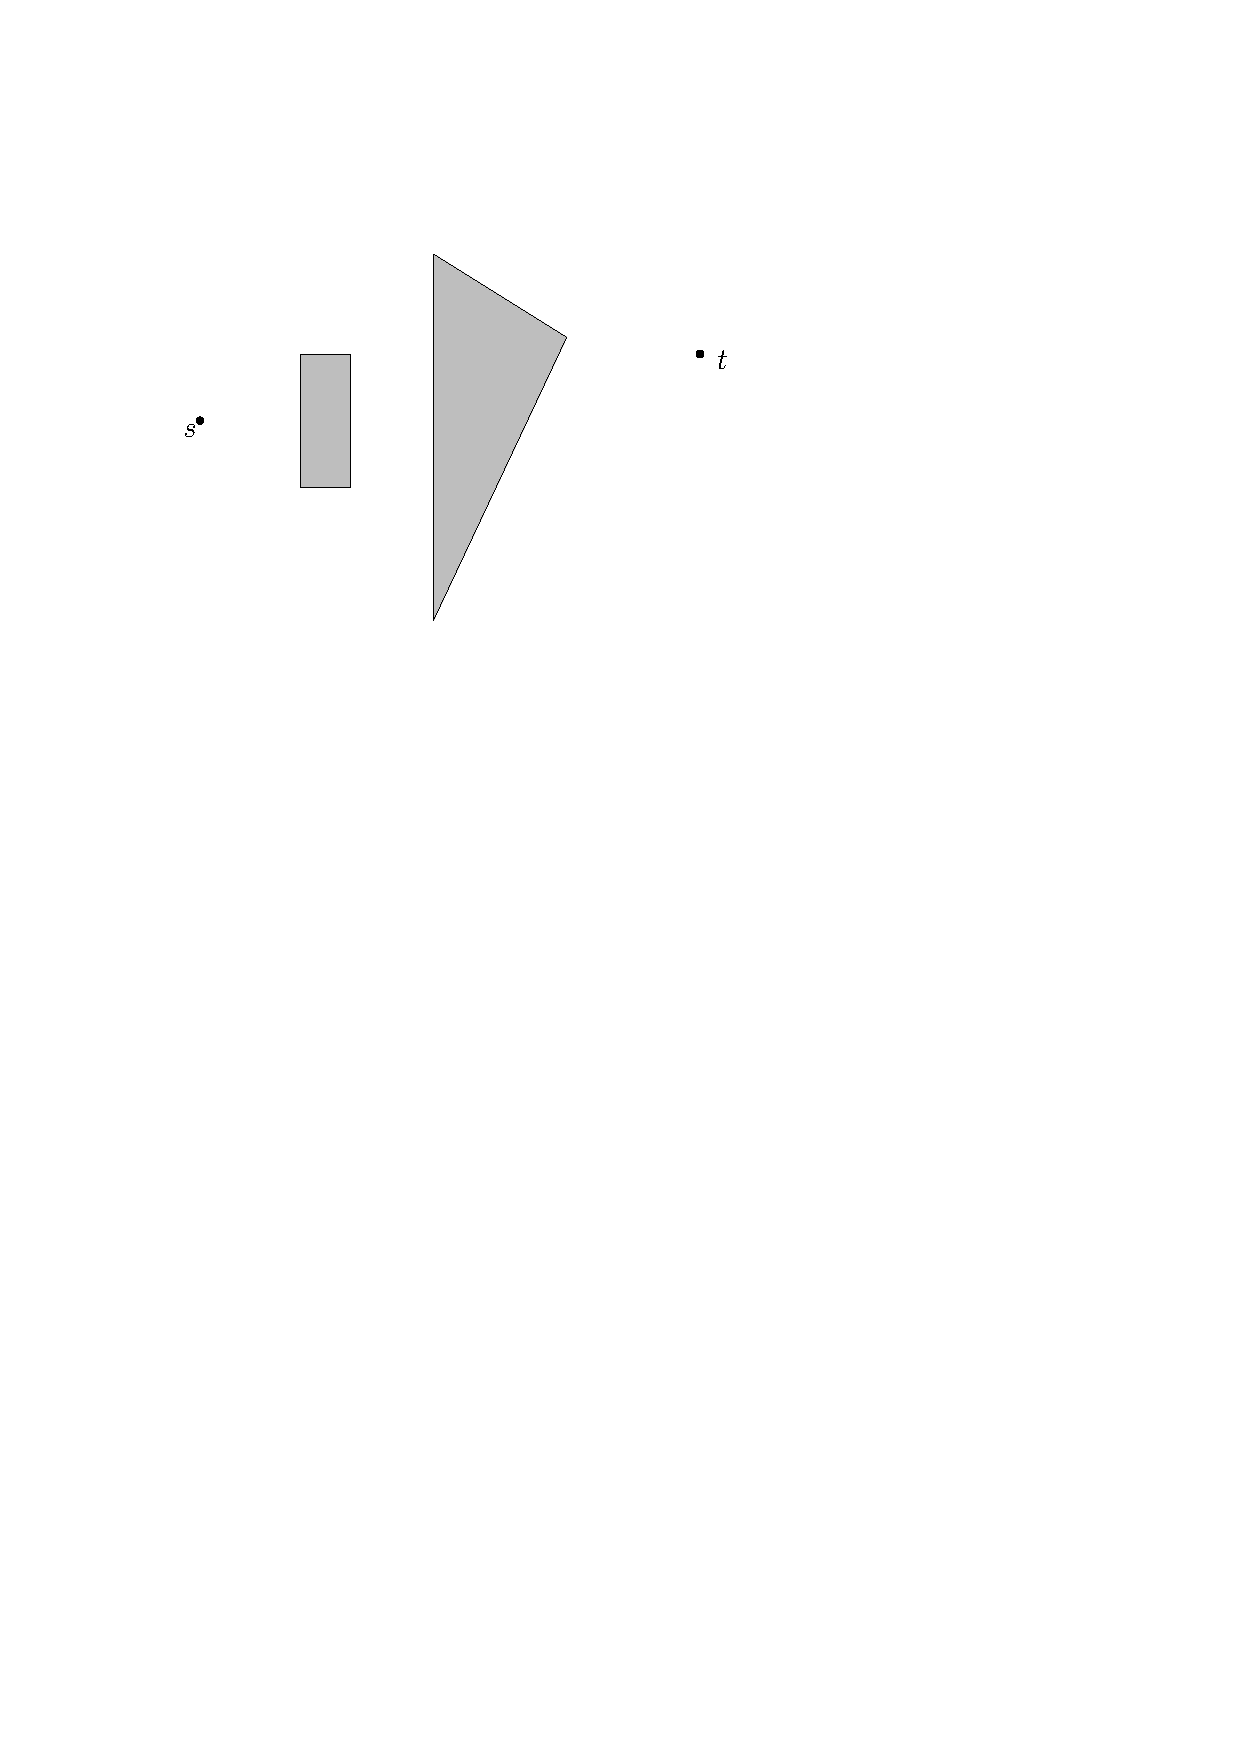
\includegraphics[width=.95\linewidth]{figures/prespm0.pdf}
  \caption{A plane with source $s$ and target $t$ with two obstacles}
  \label{fig:spmplane}
\end{subfigure}%
\begin{subfigure}{.5\textwidth}
  \centering
  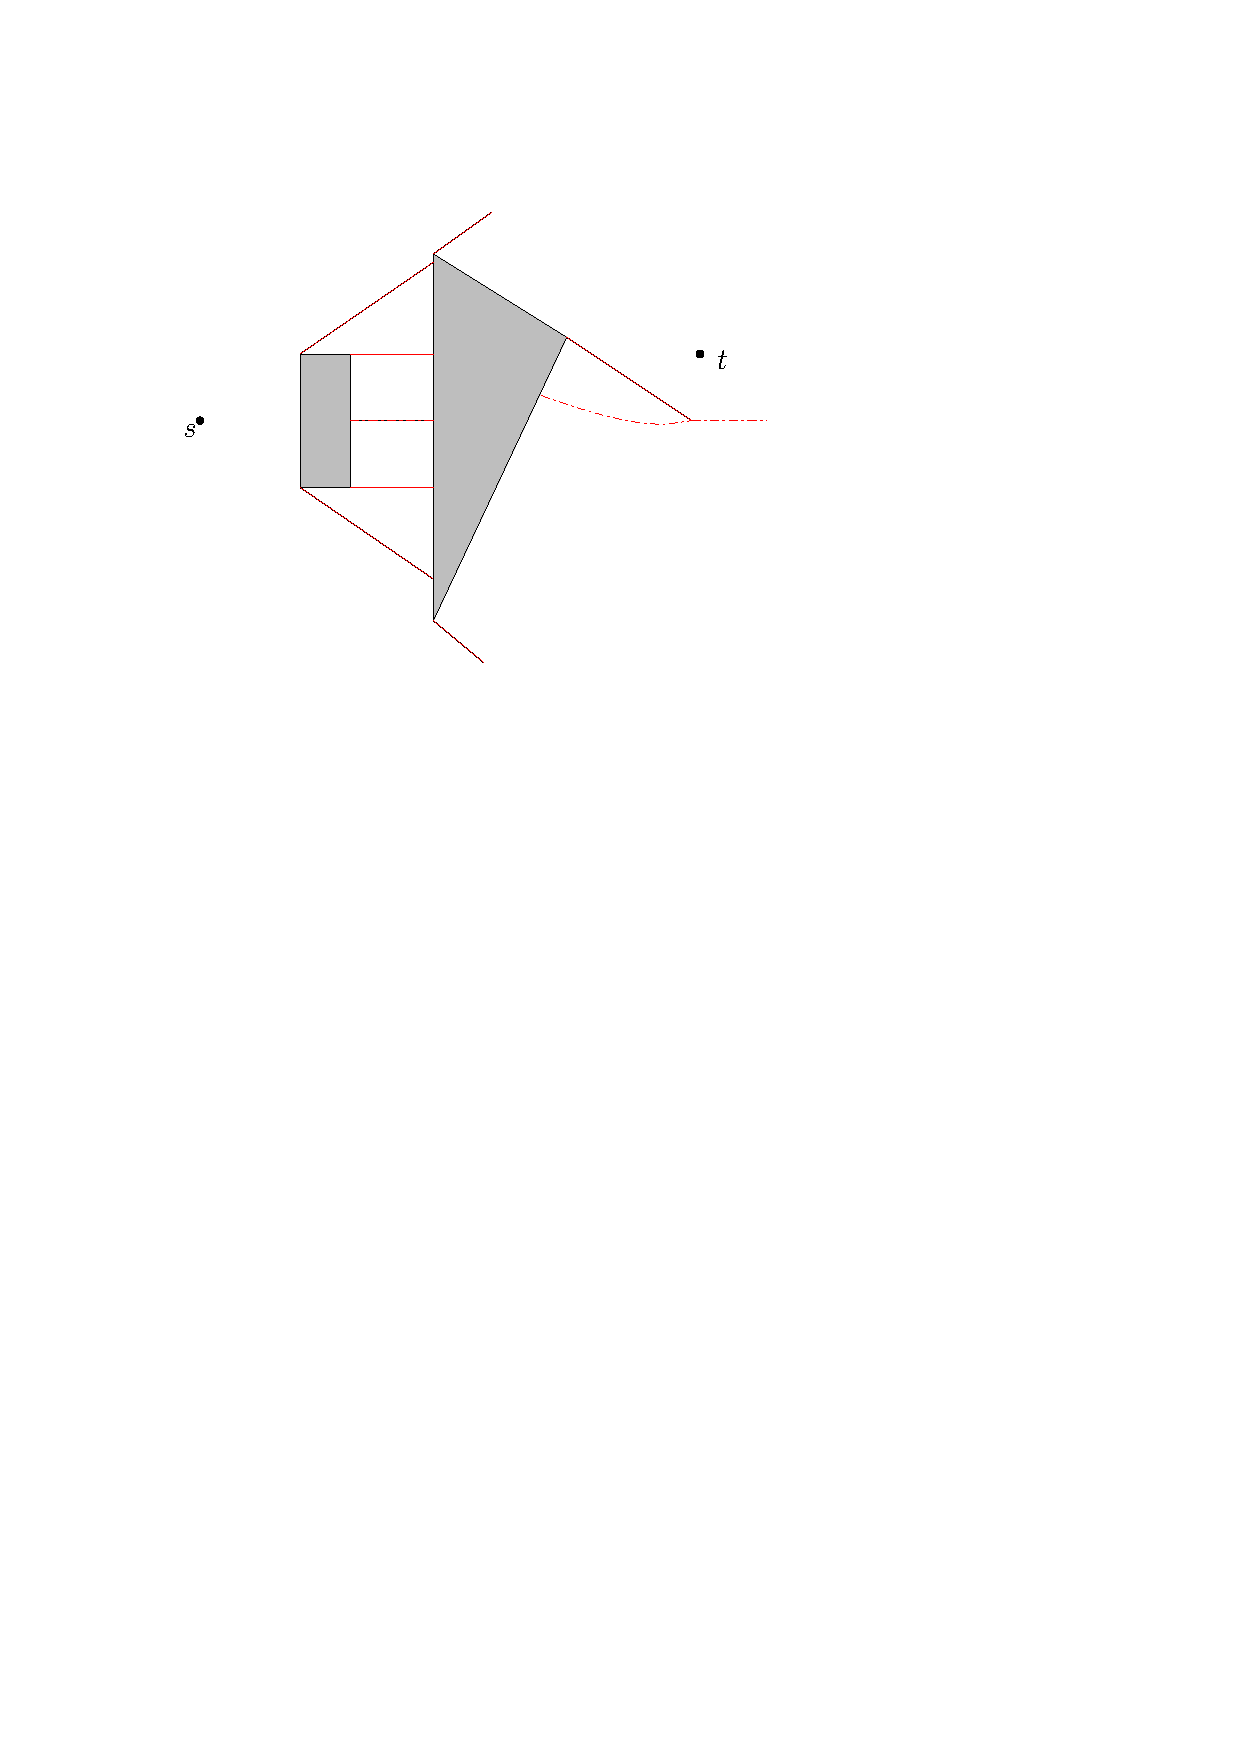
\includegraphics[width=.95\linewidth]{figures/spm0.pdf}
  \caption{A plane with the regions of $SPM_0$ drawn. The dash dotted line is the edge of two 
  		   areas where there is two shortest paths of equal length}
  \label{fig:planewithspm0drawn}
\end{subfigure}
\end{figure}

Above we see in figure \ref{fig:spmplane} a plane with $s$ and $t$ and two obstacles. Figure 
\ref{fig:planewithspm0drawn} shows a drawing of the $SPM_0$, which the unmodified 
Hershberger-Suri algorithm will calculate. 

\begin{figure}[H]
\caption{}
\centering
\begin{subfigure}{.5\textwidth}
  \centering
  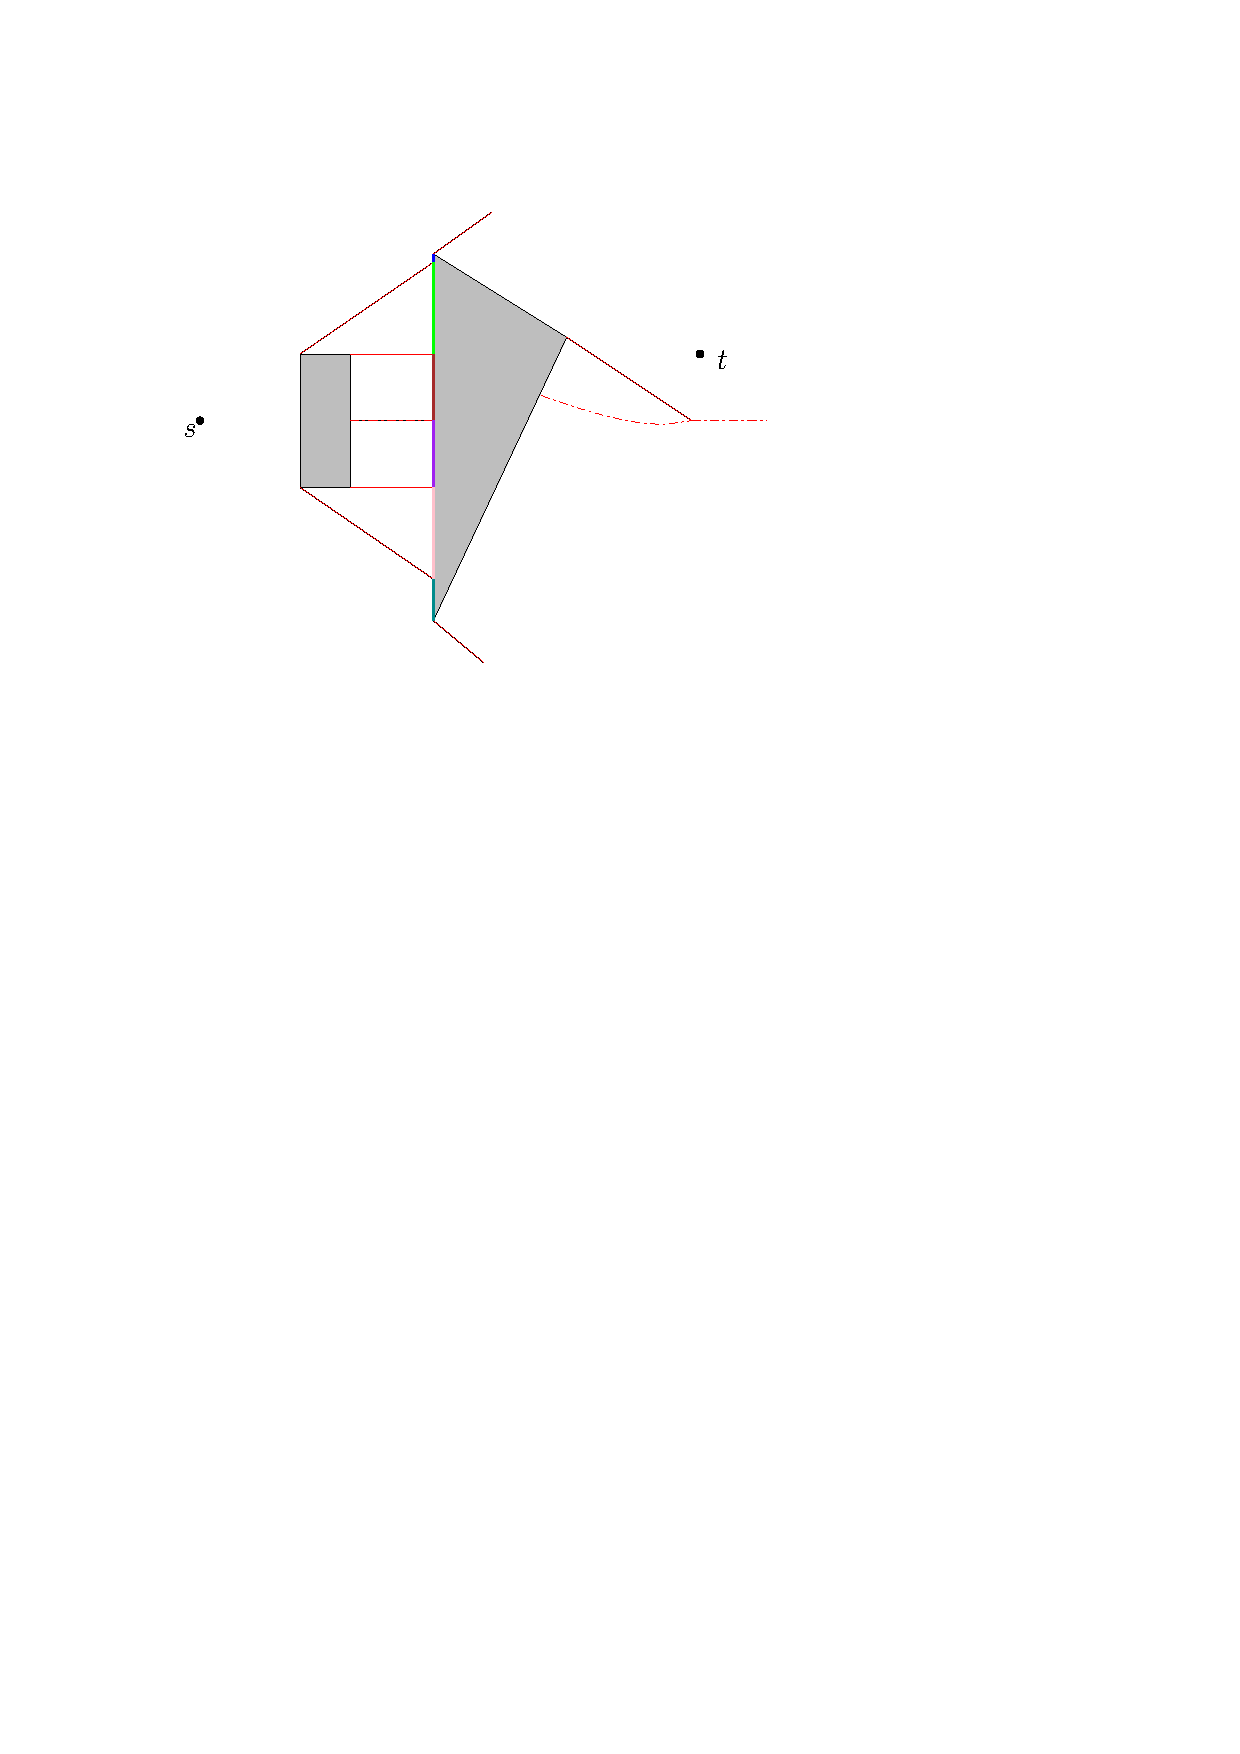
\includegraphics[width=.95\linewidth]{figures/spm0projection.pdf}
  \caption{The preparation of the modified Hershberger-Suri, which will propagate through each 
  		   color on the left most edge of the triangular obstacle}
  \label{fig:spm0projection}
\end{subfigure}%
\begin{subfigure}{.5\textwidth}
  \centering
  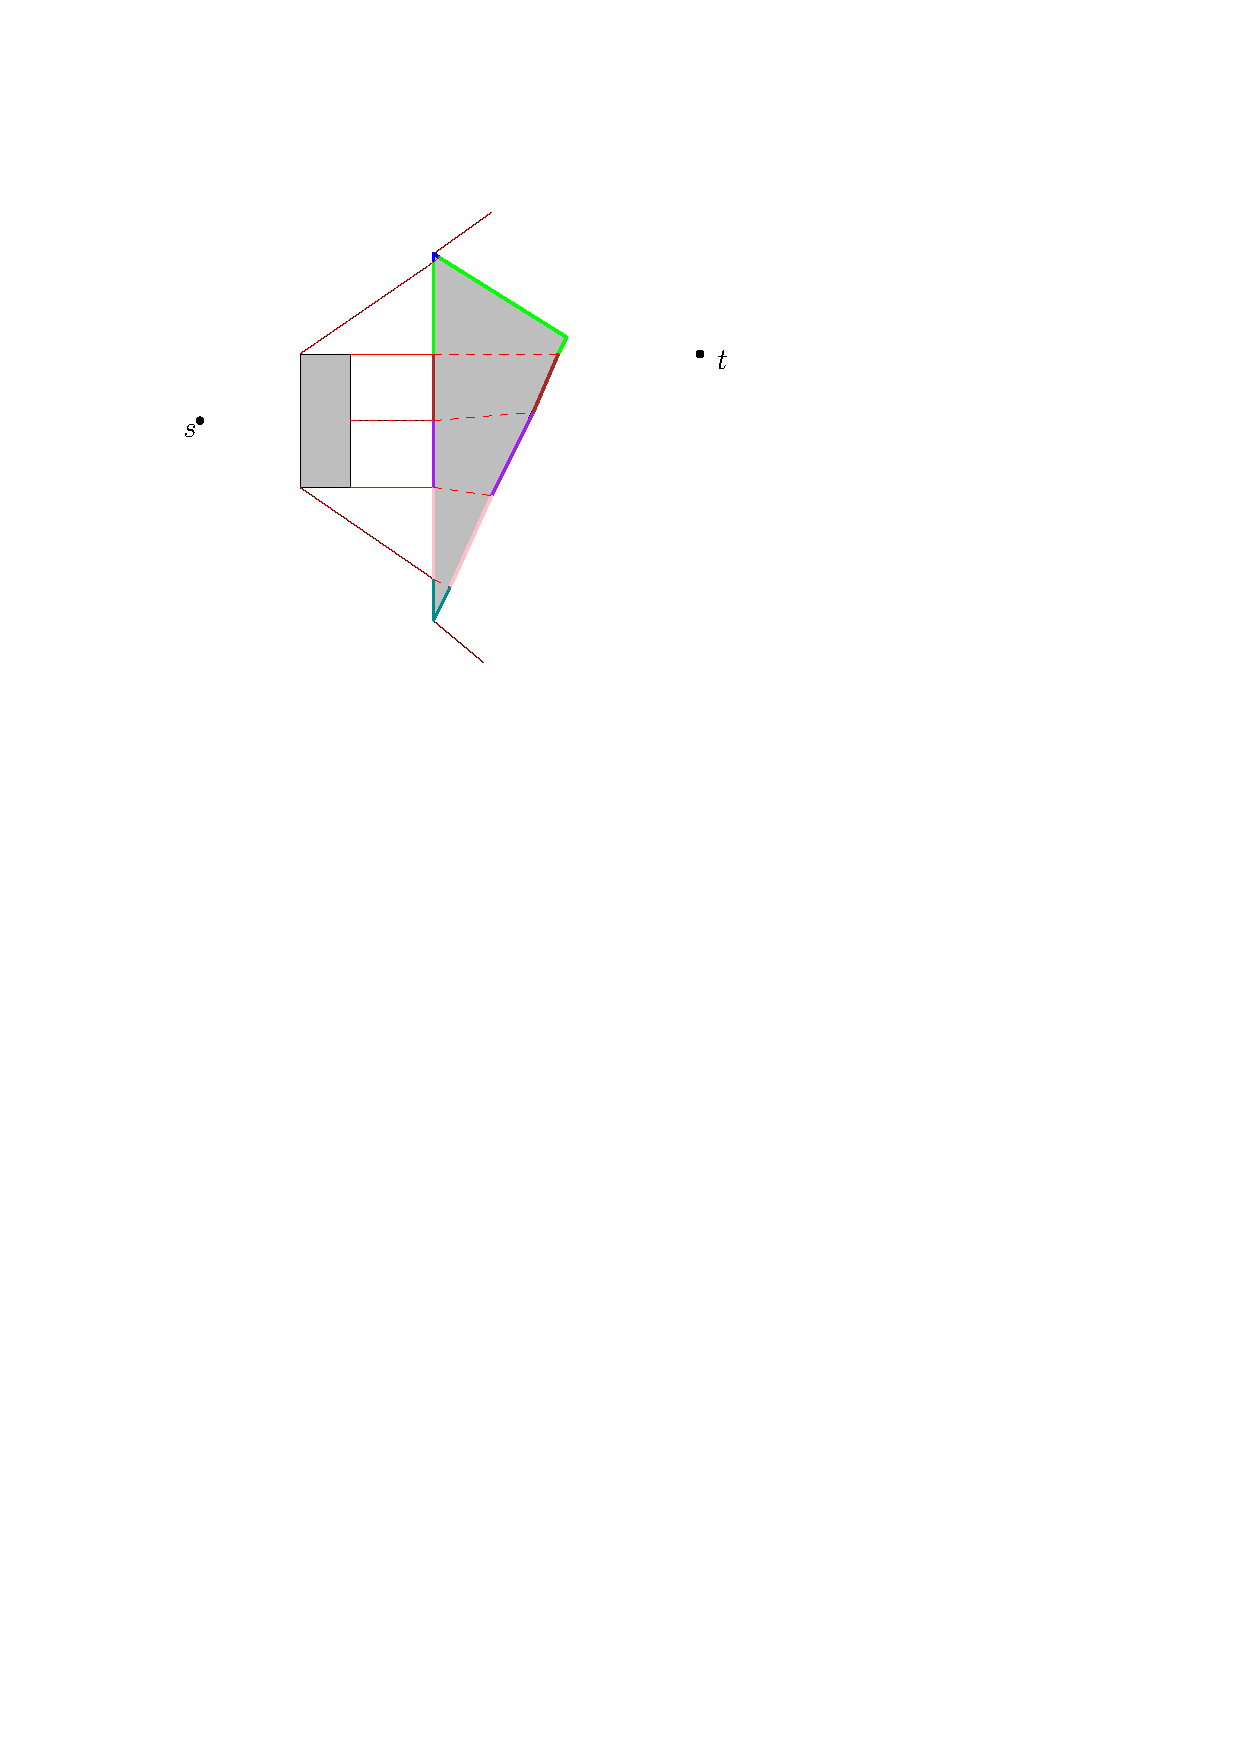
\includegraphics[width=.95\linewidth]{figures/spm1.pdf}
  \caption{the modified Hershberger-Suri algorithm propagates through the triangle to the 
  		   opposite side, where the propagation into the free space will happen for each 
           colored sub-edges as sources}
  \label{fig:spm1}
\end{subfigure}
\end{figure}

The modified algorithm needs to be able to propagate not from a source which is a point but 
from a sub-edge which can be seen in figure \ref{fig:spm0projection}. Each of the colors 
represent a "sub-edge-source" from which wavefronts will propagate the obstacle. When the 
obstacles interior has been propagated, the modified algorithm is ready to propagate the free 
space towards $t$, which we see in figure \ref{fig:spm1}. It's worth noting that the free area 
the modified algorithm needs to propagate in figure \ref{fig:spm1}, is enclosed by the the two 
red line which are collinear with $s$ and the top and bottom point of the triangle, with an 
angle of less than 180 degree. This is due to the area on the other of the wedge could be 
reached faster by just going directly from $s$ without violating an obstacle.

This process is then repeated when constructed the next level of the $SPM_i$ map. Finally we 
will have $SPM_k$ which will consist of an area where the path freely can traverse, since it 
haven't violated more than the allowed obstacles, and a $SPM_{=k}$ which consist of areas, 
where the path needs to make turns since it can't violate any more obstacles. These two areas 
are what $SPM_k$ are made of, and from this we can use the map to look up the fastest path 
from $s$ to $t$.

\chapter{Shortest path maps and their geometric properties}

\label{chapter:shortestpathmap}

This chapter is dedicated to presenting some formal definition that will help us
precisely discuss the theory in the rest of the thesis. We will also define the
shortest path map and its near relatives the shortest $k$-path map, and some properties
their properties. Finally we will present a Lemma which bounds some complexity of 
the shortest path map which will be usefull later in \ref{chapter:wavefrontpropagation}.

\section{Definitions for shortest paths and shortest $k$-paths}

We start with a trivial definition which we will expand upon.

\begin{mydef}\textbf{Path:}
Given a plane encapsulated by a polygon $\mathcal{P}$, let $s$ and $t$ be two
	points in the plane. We define a path between $s$ and $t$ to be a set of
	vertices and edges which forms a connection from $s$ to $t$.
\end{mydef}

Its trivial to see that a path with a minimum length in the case where $s$ and $t$
are the only entities in the plane will be $\overline{st}$. But we can imagine the
space being occupied not only by two points $s$ and $t$, but also with a set of 
polygons in which a path cannot pass through. We call such polygons obstacles and
we assume through out the rest of this thesis that these obstacles will be 
simple polygons. Since we will represent these with graphs we give a definition of 
simples graphs.

\begin{mydef}\textbf{Simple Graph:}
  A graph is simple if it has no loops and no two of its links join the same pair
  of vertices.
\end{mydef}

Now we might be in a situation where the path with minimum length between two point 
$s$ and $t$ isn't just $\overline{st}$ due to obstacles being placed in the way. We 
further define what space we can create our path in, and which we cannot.

\begin{mydef} 
	\textbf{Free space:}\\ 
	Let $\mathcal{O}=\{O_1,O_2,...,O_k\}$ be a
	family of simple polygons which will act as obstacles in the interior of an
	encapsulating polygon $\mathcal{P}$. We define the free space to be
	$\mathcal{FS}=\mathcal{P}\setminus\mathcal{O}$, that is the plane of the
	encapsulating polygon minus the interiors of all obstacle polygons.
\end{mydef}

The final $O(k^2 \cdot n \log n)$ algorithm that we will be examining will  
need the obstacles to be convex, which are defined as follows: 

\begin{mydef}
	\textbf{Convex Polygons:} \\ 
	A convex polygon is a simple polygon (not self-intersecting) in which no
	line segment between two points on the boundary ever goes outside the
	polygon. In a convex polygon, all interior angles are less than or equal to
	180 degrees, while in a strictly convex polygon all interior angles are
	strictly less than 180 degrees.
	\cite{Bisector-collinearity-convexPoly} 
\end{mydef}

We are only allowed to make paths between $s$ and $t$ in the free space, which we 
will denote as legal paths.

\begin{mydef}
	\textbf{Legal Path:}\\ 
	We define a path between two vertices to be
	legal if it lie entirely in the free space. That is a legal path is disjoint
	from the interiors of all potential obstacle polygons in the plane.
\end{mydef}

Now we are ready to define out legal shortest path between our two points $s$ and 
$t$

\begin{mydef}
	\textbf{Euclidian shortest path:}\\ 
	The legal path of minimum total length connecting the two endpoints is a 
    shortest path.  
\end{mydef}

We define a path which is not legal to be violating, or having a number of
violations, equal to the number of obstacles in which the path will pass
through. We will not only deal with shortest paths which have no violations,
but also shortest path which allow up to $k$ violations.

\begin{mydef}
	\textbf{Shortest k-path}
	The path of minimum total length which violates at most $k$ obstacles.
\end{mydef}

Through out this thesis we will use use the notation of $\pi(s,t)$ to denote the 
shortest paths connecting two points $s$ and $t$ in the case where no obstacle 
violation is allowed. The length of any path in	$\pi(s,t)$ is the shortest path 
distance between $s$ and $t$, denoted $d(p,q)$. If the shortest path between $s$ 
and $t$ is the line segment $\overline{p,q}$, then $p$ and $q$ are said to be 
visible. 

\begin{mydef}
	\textbf{Visibility between points:}
    We define two points $s$ and $t$ to be visible to each other if $s$ and $t$ are 
    connectible with the path $\overline{st}$ which is either legal, or in the case 
    of violations have less that the allowed $k$ violations.
\end{mydef}

The notion of shortest path distance between two sets of points $X$ and $Y$ is 
denoted as $d(X,Y)$ and is the minimum $d(x,y)$ over all pairs of points $x\in X$ 
and $y \in Y$. \cite{HershbergerS99} \\

We call a path violating of at most $k$ obstacles a \textit{$k$-path}, generalizing 
on the traditional obstacle-free path, which is a 0-path. We use the notation of 
$\pi_k(p)$ to be the shortest path in this case where the path can pass through up 
to $k$ obstacles from a \textit{fixed source} $s$ to the point $p$. When reasoning 
about a path with exactly $k$ crossing we denote this as an $(=k)$-path. And 
equally we use $d_k(p)$ to denote the length of the shortest path from the fixed 
source $s$ in the case of up to $k$ obstacle violations. The reason we use a 
separate notation in the case of obstacle violation is that shortest 0-path 
problem with origination at a common source point $s$ cannot intersect, by the 
triangle inequality\cite{HershbergerKS17}

\begin{mydef}
	\textbf{Triangle Inequality:} \\ 
	Let $A$ and $B$ be points in a $\mathbb{R}^n$ space and let $|AB|$ denote
	the distance between $A$ and $B$.  Then the triangle inequality states that
	for three points $A,B,C\in\mathbb{R}^n$ \cite{metricspaceandpoints}
	$$|AB|\leq|AC|+|BC|$$
\end{mydef} 
\begin{figure}[H] 
	\centering
	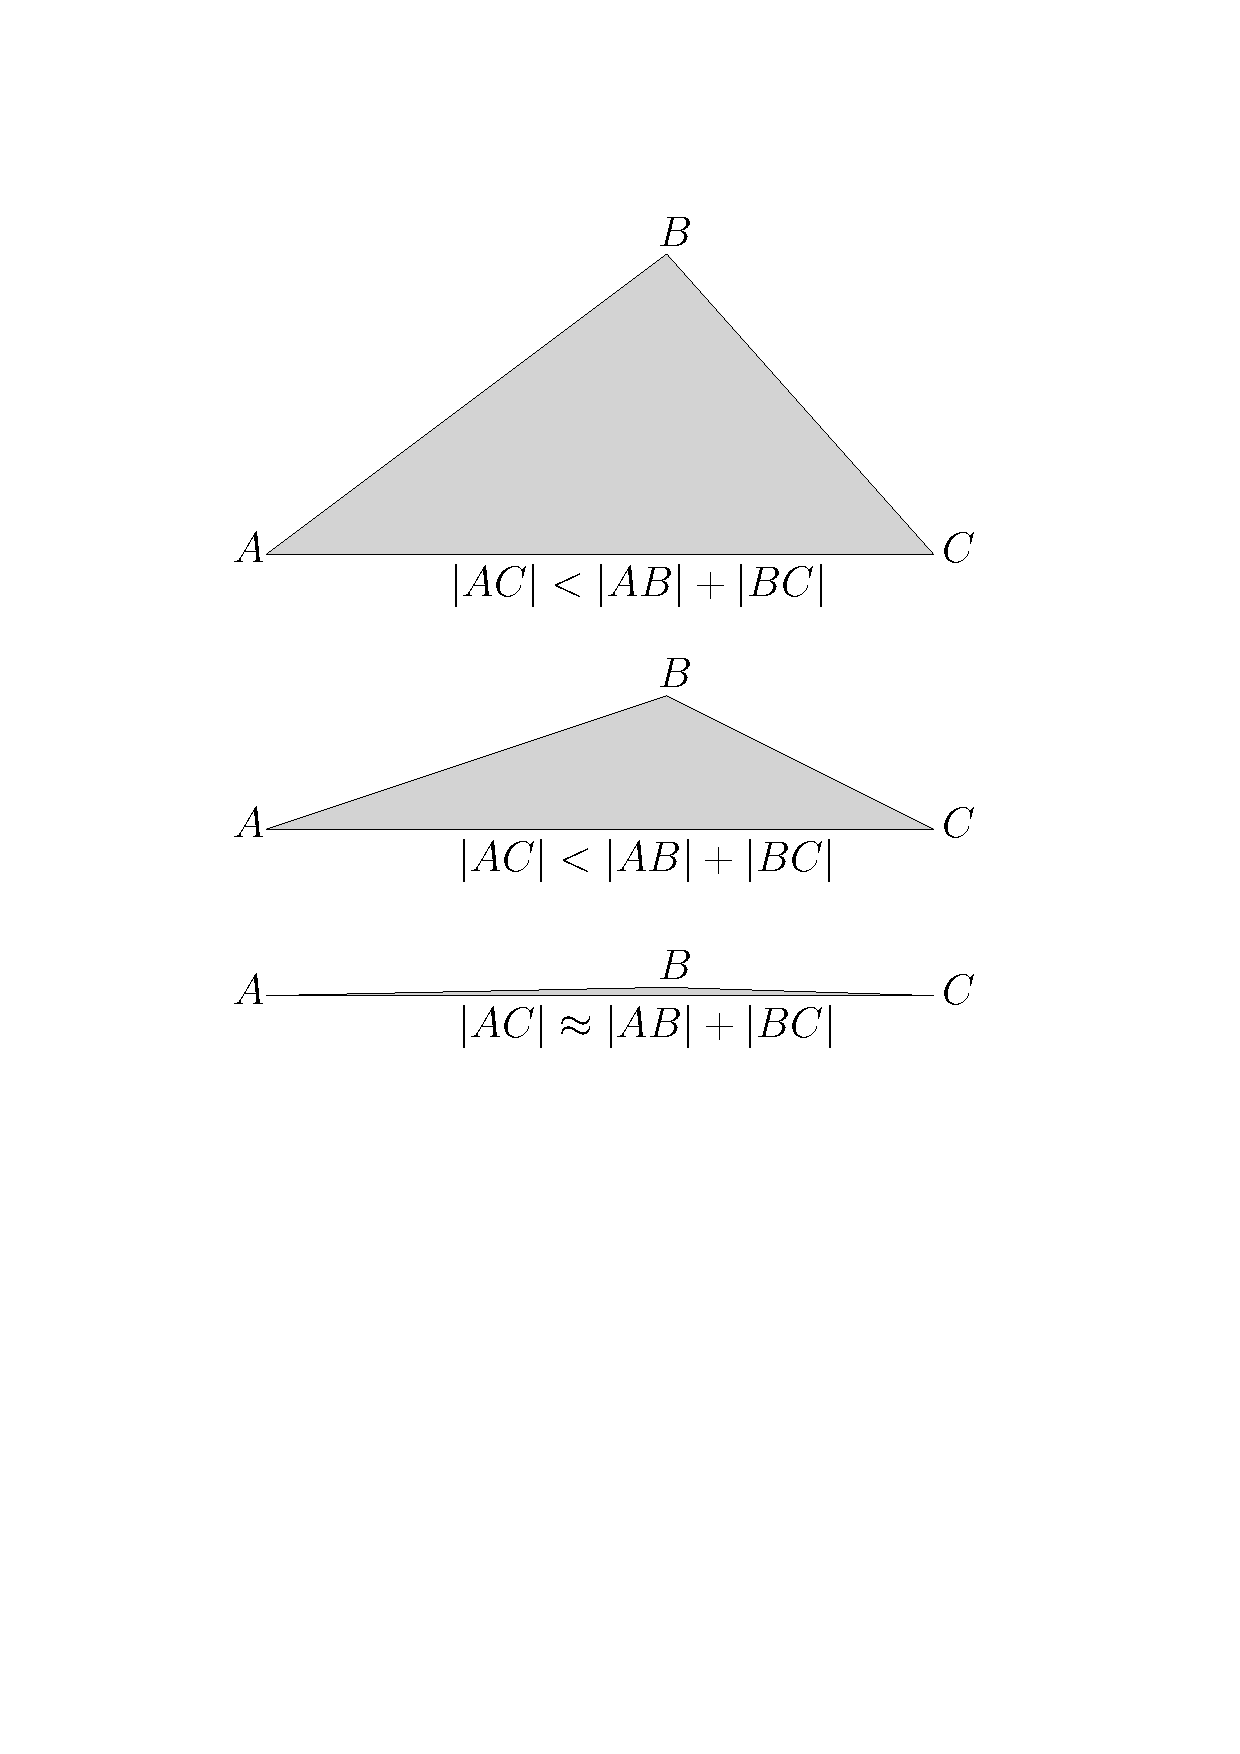
\includegraphics[width=5cm]{figures/TriangularInequality.pdf}
	\caption{Triangular Inequality approaching equality}
	\label{fig:TriangularInequality} 
\end{figure}


\section{Shortest path map and shortest $k$-path map}

This section will briefly introduce the reader to the concept of shortest path map
and shortest $k$-path map and som basic properties of these.

We begin this section with a definition of a predecessor which is essential to understand
what a shortest path map is

\begin{mydef}
	\textbf{Predecessor:} \\ 
	The predecessor of an arbitrary point $p$ is defined as a vertex in the plane which is 
	adjacent to $p$ in $\pi(p,s)$. These vertices also include the source $s$. A predecessor of
	$p$ is necessarily visible from $p$. If $p$ and $s$ are mutually visible,
	then $s$ is a predecessor of $p$. \cite{HershbergerS99} 
\end{mydef}

next we give the definition of a shortest path map

\begin{mydef}
	\textbf{Shortest Path Map:} \\ 
	The shortest path map  of a
	particular source point s, denoted $SPM(s)$, is a subdivision of the plane
	into two-dimensional regions such that all the points in one region have the
	same, unique predecessor\cite{HershbergerS99}. 
\end{mydef}

An example of an $SPM$ can be seen in figure \ref{fig:exampleofspms} blow

\begin{figure}[H] 
	\centering
	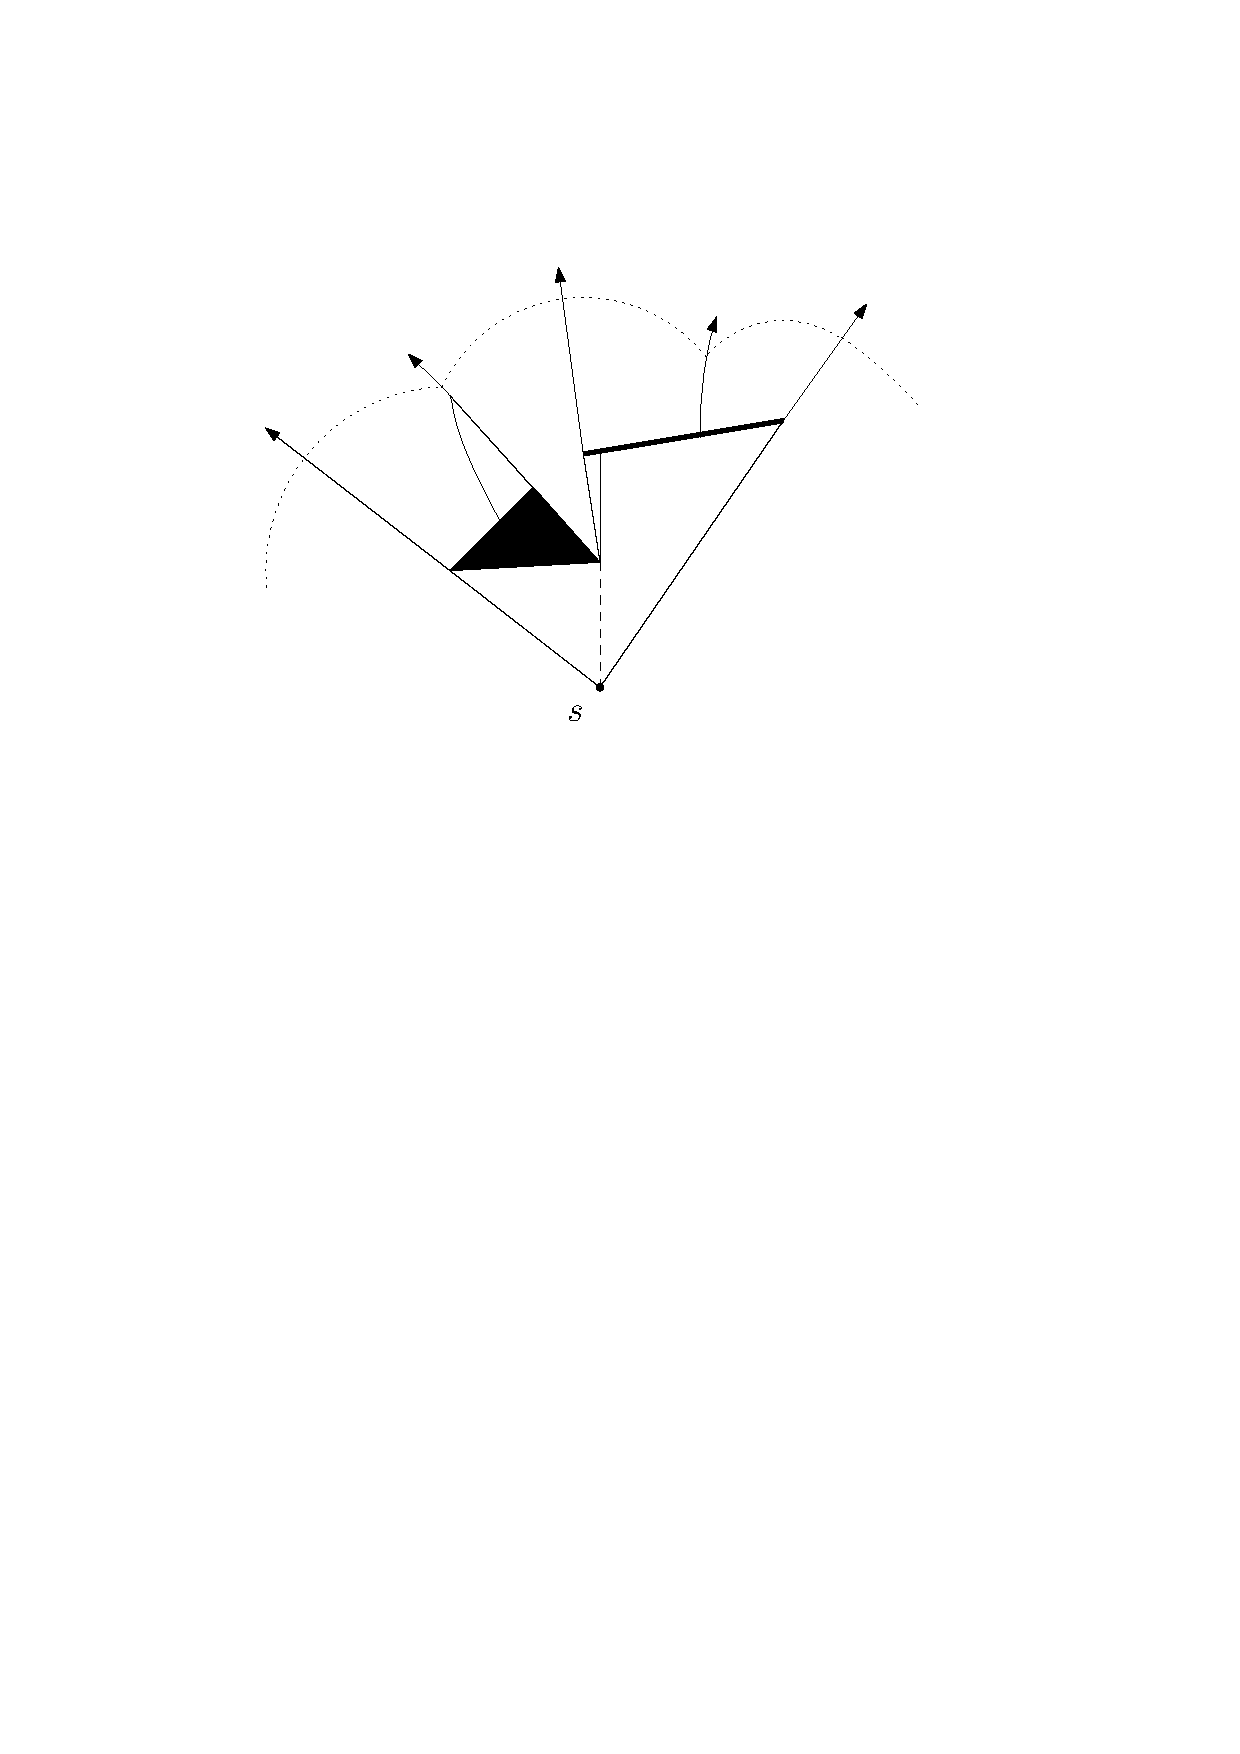
\includegraphics[width=0.65\textwidth]{figures/exampleofspms.pdf}
	\caption{An example of an $SPM$ build around $s$ with where the area between
	         the arrows and fully drawn lines shows the regions in the plane with
	         the same predecessors.}
	\label{fig:exampleofspms} 
\end{figure}

The figures shows the $SPM$ build around $s$ as the source, and the different obstacles in the plane. 
Since a shortest path only needs to turn at the vertices of the obstacles, by triangular inequality, 
the vertices of obstacles naturally constitute the unique predecessors of the points within the different 
regions marked by the fully drawn lines. Here the lines will extend until the meet the encapsulating 
polygon $\mathcal{P}$ an then be fully enclosed. The dashed lines show the shortest path from a region 
$s$ or to the preceding region. It should be noted that these fully drawn line constitutes bisectors 
(which will explained in later chapter) and there point on the line have a equal distance to $s$ through 
either of the regions which the bisector acts a border between. It should therefore be noted that in the 
case of the $SPM$ there may multiple shortest paths to points in the plane, in which case one just chooses 
one of them.

The distance to a point $p$ in the $SPM$ is calculated by finding the weight from $s$ to $p$

\begin{mydef}
	\textbf{Weight:} \\ 
	We define weight of an vertex (including obstacle vertices) to be
	its shortest path distance to the source $s$. Given an arbitrary point $p$
	in free space, its weighted distance to a visible vertex $v$ is defined as
	$$d(s,v) + \left| \overline{vp} \right|$$
	that is the straight-line distance from $v$ to $p$ plus the shortest path 
	distance from $s$ to $v$.
	\cite{HershbergerS99} 
\end{mydef}

Next we move on to the definition of $k$-predecessors and the shortest $k$-path map

\begin{mydef}
	\textbf{$k$-predecessor}\\ 
	Given a shortest $k$-path $\pi_k(p)$, we define the \textit{predecessor of
	p} to be the vertex (including $s$) that is adjacent to $p$ in
	$\pi_k(p)$\cite{HershbergerKS17}. 
\end{mydef}

\begin{mydef}
	\textbf{Shortest k-path map}(Definition 9 in \cite{HershbergerKS17})\\
	The partition of free space into connected regions with the same
	$k$-predecessor is called the \textit{shortest k-path map}, and is denoted
	by $SPM_k$. The subset of $SPM_k$ for which the shortest path $\pi_k(p)$ to
	every point $p$ has exactly $k$ crossings is called the shortest $(=k)$-path
	map and denoted by $SPM_{=k}$. 
\end{mydef}

It is quite easy to see that a $SPM$ is the same as an $SPM_{=0}$, we will therefore use $SPM$ when 
dealing with the Hershberger-Suri algorithm in chapters \ref{chapter:conformingsubdivision} and 
\ref{chapter:wavefrontpropagation}, and $SPM_{=0}$ when dealing with the computing of $SPM_k$ in
chapter \ref{chapter:shortestpathobstaclesviolation}.

We saw with the $SPM_0$ map that each predecessor to an region always where on the boundary on said
region, this isn't necessarily the case for a $SPM_k$. Further more multiple regions in $SPM_k$ may 
have the same predecessor see figure \ref{fig:1predecessor}.

\begin{figure}[H] 
	\centering
	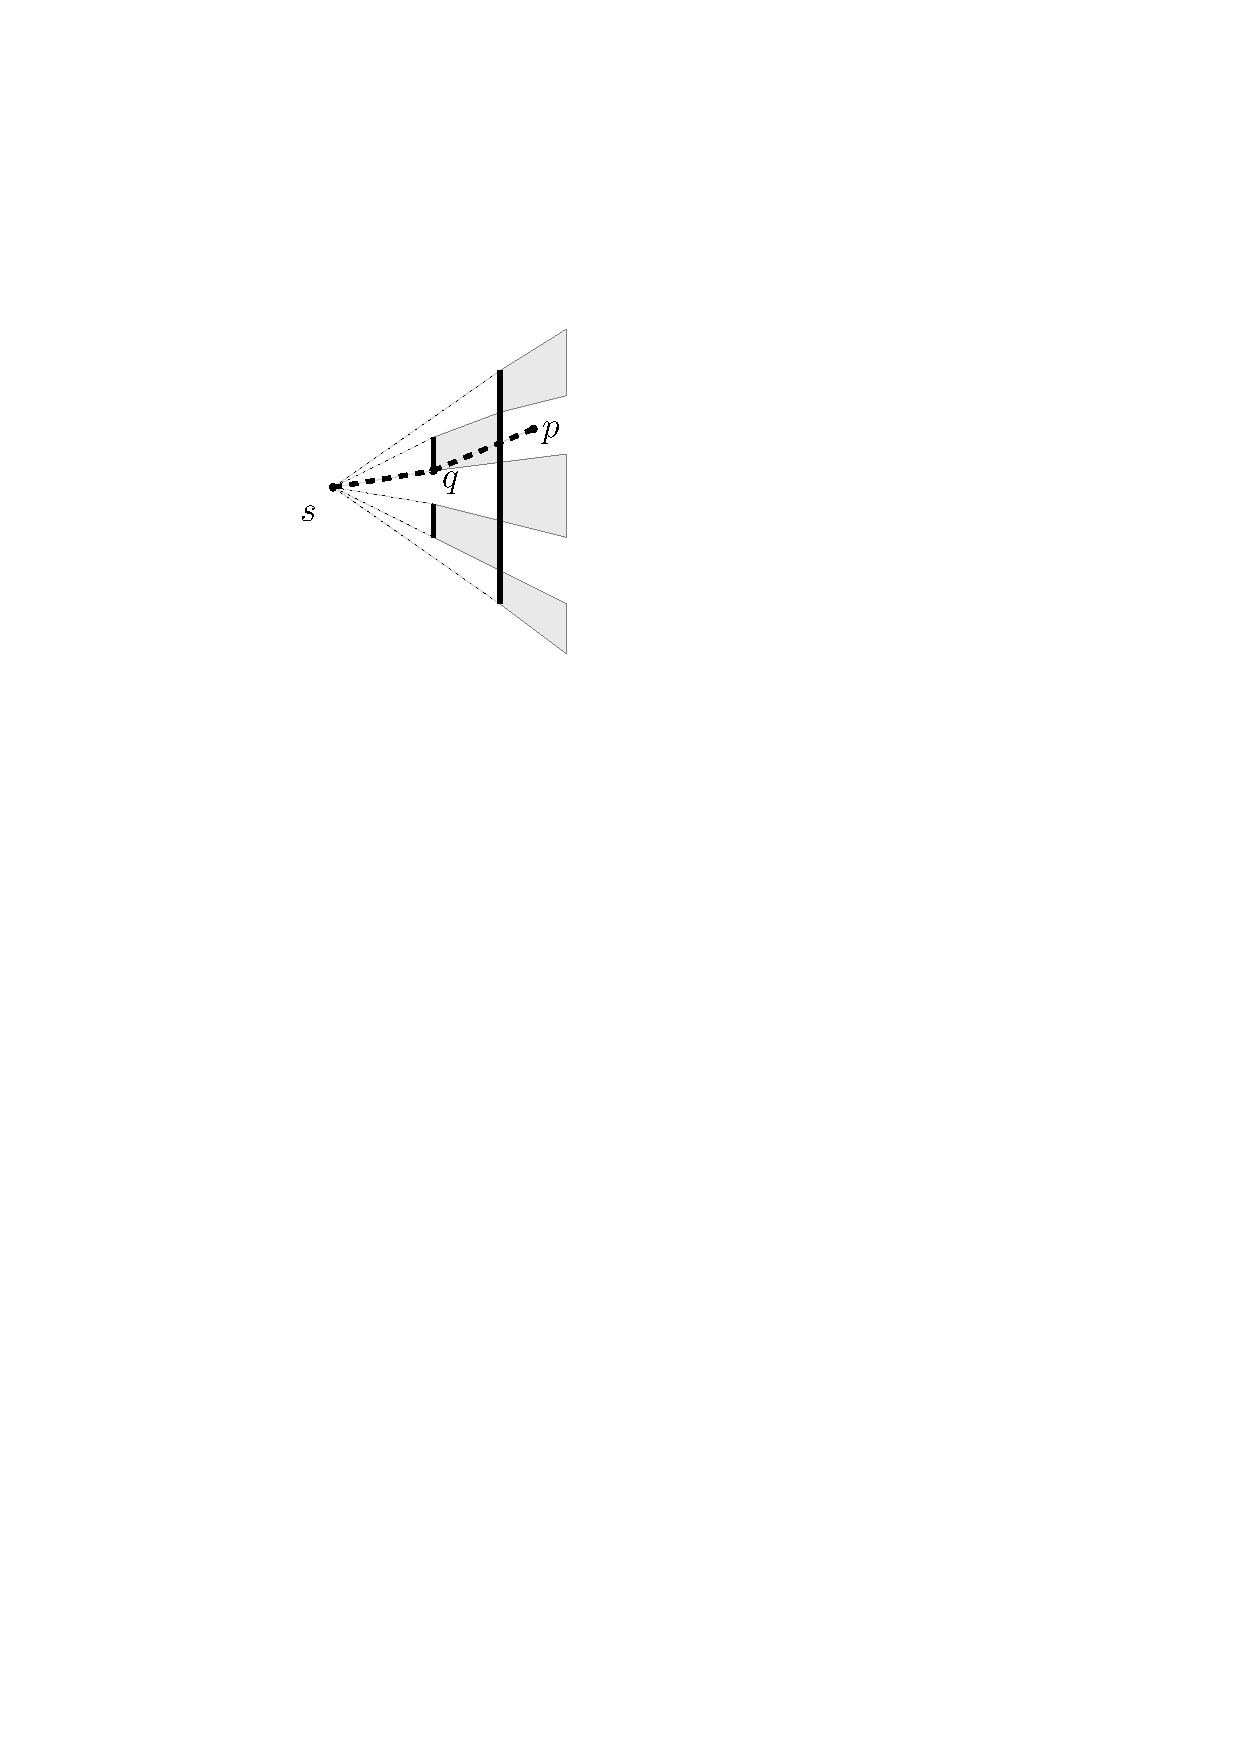
\includegraphics[width=0.4\textwidth]{figures/1predecessor.pdf}
	\caption{Here we present a $SPM_1$ map, where we the fat lines are obstacles.}
	\label{fig:1predecessor} 
\end{figure}

Here we see that the shortest path from $s$ to $p$ goes through point $q$ which lies outside the region
in which $p$ is. So we need to maintain additional information with polygon vertices to disambiguate the 
predecessor relation. So suppose we have a live segment $\overline{vp}$ between to vertices which crosses
$(k-1)$ obstacles for some $0 \leq i \leq k$, then the length $d_k(p)$ of $\pi_k(p)$, is defined as
the sum of the length of the $i$-path to $v$ and the length of segment $\overline{vp}$. So in the context
of figure \ref{fig:1predecessor}  we have $\overline{qp}$ crosses $(k-1)$ obstacle in the relation of $0 \leq
1 \leq k = 1$, which leaves the $k - 1 = 0$ obstacles left which we can cross. The $0$-path to $q$ is the
direct path $\overline{sq}$, where we have the total shortest path.

So for a point $p$ in $SPM_{=k}$, we identify the $k$-predecessor of $p$ by the pair $(v,i)$, where $v$
is a vertex of $\mathcal{P}$ and $i \in \{0,1,..,k\}$ such that $d_k(o) = d_i(v) + |\overline{vp}|$ and the
segment $\overline{vp}$ crosses $(k-i)$ obstacles \cite{HershbergerKS17}.

Neat property of the $SPM_k$ is we devide it into two parts, a $V_{k-1}$ path which is the region consisting of
$k-1$-visible points, which is starshaped, and the $SPM_{=k}$ part. The concept of $V$ areas can be seen in
figure \ref{fig:regions}.

\begin{figure}[H] 
	\centering
	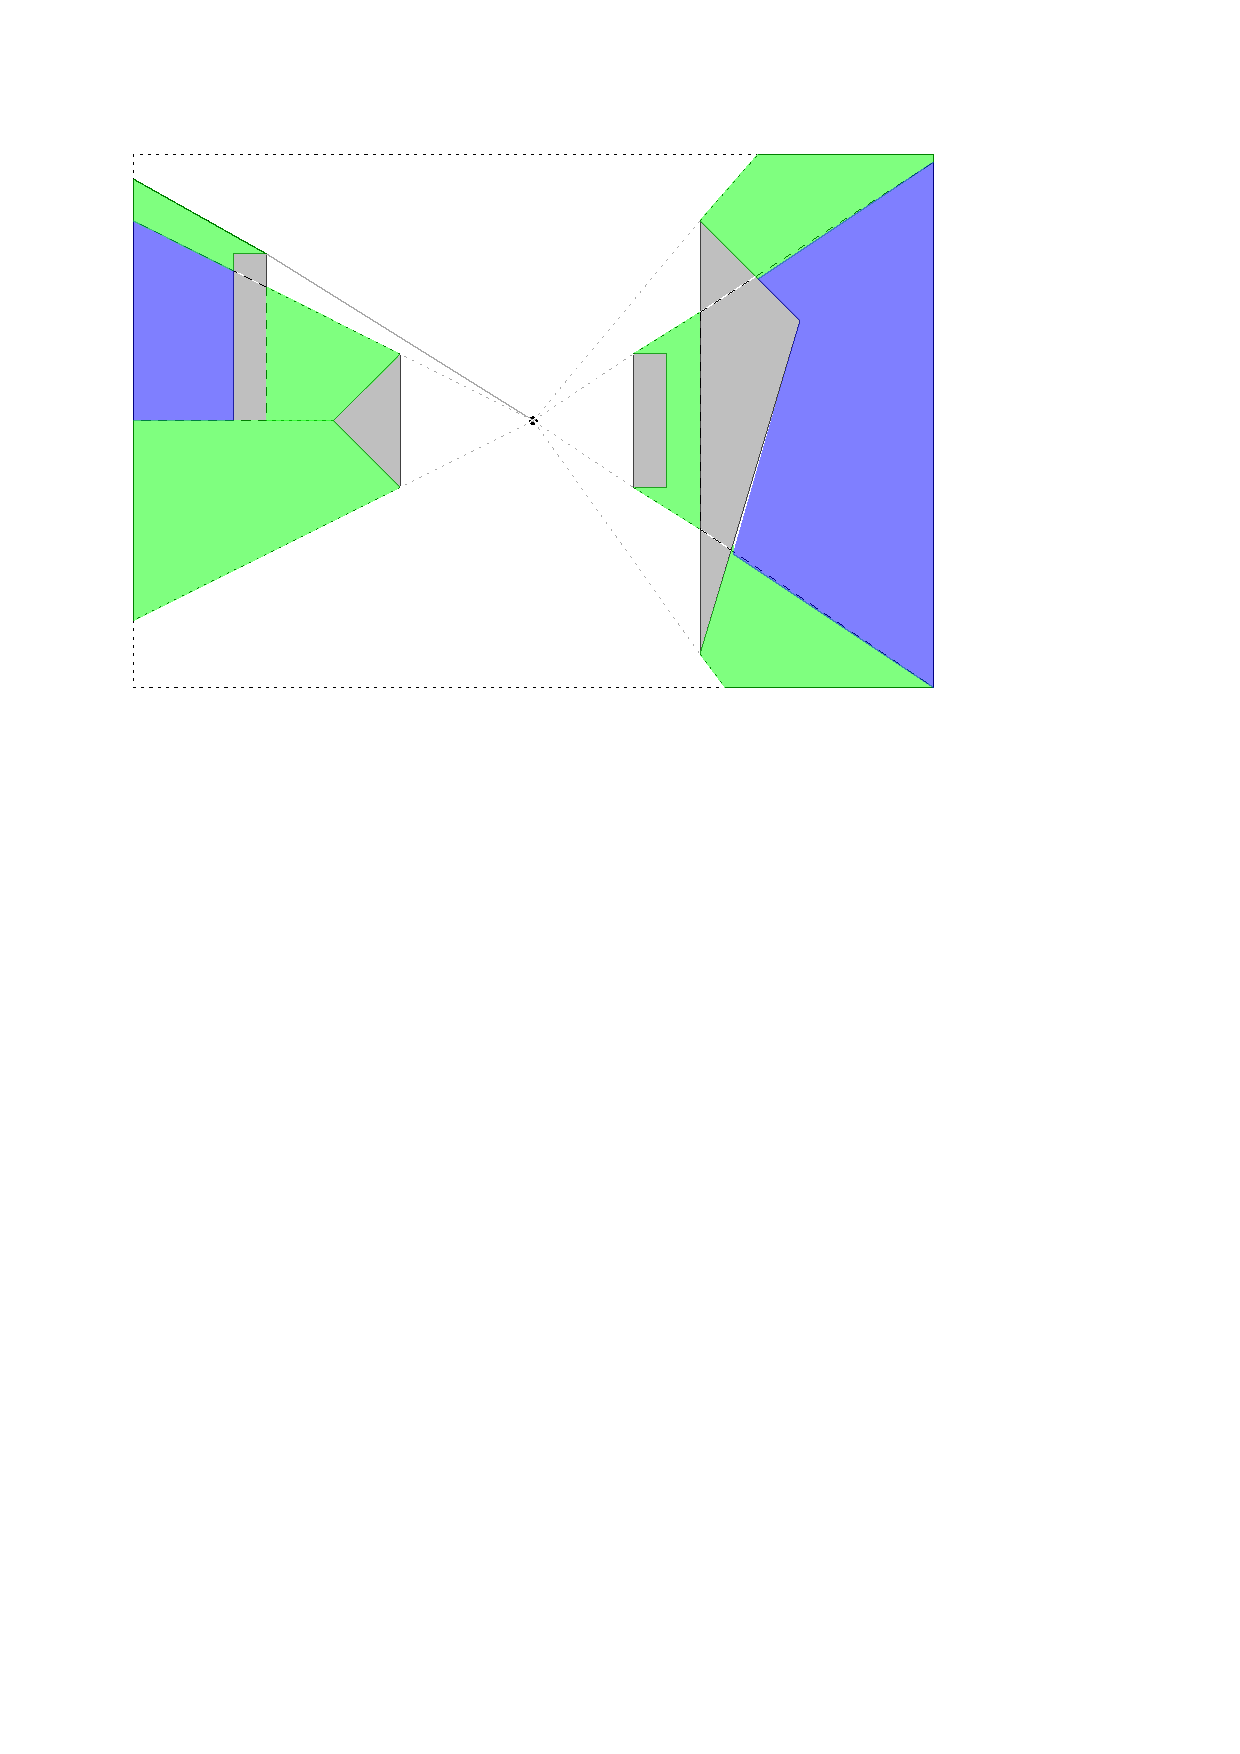
\includegraphics[width=0.8\textwidth]{figures/regions.pdf}
	\caption{Here the boundary of $V_1$ is marked with dashed lines, while the region of $V_0$ is shown with 
	         dotted lines. $V_1$ is further shown with blue and the $V_1 \setminus V_0$ is shown with green.}
	\label{fig:regions} 
\end{figure}

\section{Complexity of $SPM$ map}

Here follows a Lemma which will be usefull for bounding the number of hyperbolic arcs in the proof 
of Lemma \ref{lemma:4.12} in chapter \ref{chapter:wavefrontpropagation} but first we define what
a star-shaped polygon is.

\begin{mydef}[Star-shaped polygon]\cite{PreparataS85}
	\label{star-shaped}
	A simple polygon $P$ is star-shaped if there exists a point $z$ not external
	to $\mathcal{P}$ such that for all points $p$ of $\mathcal{P}$ the line segment 
	$\overline{zp}$ lies entirely within $P$. The locus of the points $z$ having the 
	above property is the \emph{kernel} of $\mathcal{P}$.
\end{mydef}

\begin{Lemma}[Lemma 3.2]
	\label{lemma:3.2}
	The shortest path map $SPM(s)$ has $O(n)$ vertices, edges and faces. Each
	edge is a segment of a line or a hyperbola
\end{Lemma}
\begin{proof}
	Note that each face $SPM(s)$ is star-shaped (see definition
	\ref{star-shaped})
	with the unique predecessor vertex for the face, and the predecessor is in
	the kernel of the face.
	The idea behind this proof is to show that each obstacle vertex is a
	predecessor vertex for at most one face in $SPM(s)$.
	Consider a vertex $u$ that is the predecessor of a face $F$ and let
	$pred(u)$ be the set of predecessors of $u$, this is a set because there can
	be multiple predecessors. Observe that $d(s,u)=d(s,v)+|\overline{uv}|$ for
	any $v\in pred(u)$, since the distance $d(s,u)$ can always be rewritten as
	the distance to from $s$ to $u$'s predecessor, and a straight line from the
	predecessor to $u$ since your predecessor is always visible from a point.

	If a point $p$ is visible from a vertex $v \in pred(u)$ with $v$, $u$, $p$ 
    not being collinear, then $p$ cannot have $u$ as its predecessor. This is 
    due to the triangle inequality, where it is always shorter to take the direct 
    line instead going by another point.


	Consider the subset of the free space that is visible from $u$
	but not visible from $v\in pred(u)$. Let $R(u,v)$ denote the component of
	this subset that is incident to $u$. Then $R(u,v)$ lies in an
	angular angle around $u$ of less than 180$^\circ$. Define
	\begin{align}
		R(u) =  \bigcap_{v\in pred(u)} R(u,v)
	\end{align}

	Clearly $F \subseteq R(u)$, since the area $R(u)$ is the area that is
	incident to $u$, and not visible from any predecessor $v\in pred(u)$ 
	
	Then the claim is that there is at most one face of
	$SPM(s)$ in $R(u)$ with $u$ as its predecessor. 
	
	We do this by contradiction: 
	Suppose there were two faces
	$F_1$ and $F_2$ both having $u$ as their unique predecessor. The faces $F_1$
	and $F_2$ must have exactly one point in common, the vertex $u$. In the space
	between $F_1$ and $F_2$ there is a point $p$, there have to be a point here,
	otherwise they would be the same face. The point $p$ is arbitrarily close to $u$ with
	predecessor $z$ such that $z$ is distinct from both $u$ and $pred(u)$. In
	other words $d(s,u)+|\overline{up}|>d(s,z)+|\overline{zp}|$. However as $p$
	moves towards $u$ the difference in the distance shrinks and finally
	$d(s,u) = d(s,z)+|\overline{zu}|$. But then $z$ must be a predecessor of
	$u$. This means that $F_1$ and $F_2$ is part of the same face, contradicting
	the hypothesis. Thus a vertex $u$ is a predecessor of at most one face in
	the shortest path map.

	Finally to prove the linear upper bound on the size of the shortest path
	map, recall that the number of obstacle vertices is $n$ the remaining
	vertices border at least three faces of $SPM(s)$ (for this argument we count
	the obstacle polygons as faces of the shortest path map). Since the number
	of faces is $O(n)$, Eulers formula for planar graphs implies that the total
	number of vertices is also $O(n)$. This completes the proof
\end{proof}


\chapter{Conforming subdivision}

\label{chapter:conformingsubdivision}

The following chapters result are due to Hershberger and Suri\cite{HershbergerS99}. 
We will present the main theory behind a conforming subdivision, 
and an algorithm for computing it, and The implementation details for a $O(n \log n)$
implementation.

Given a plane with obstacles, we could view this as a plane with holes in it, which we 
cannot enter. These holes are made of the obstacles occupying the space. So here the notion 
of free space is the plane minus the interior of the obstacles. This free space is where the 
unmodified Hershberger-Suri would find a shortest path, that is a shortest path without 
violations. One of the key ideas for calculating the shortest path map, which we need to 
find the shortest path, is the notion of a conforming subdivision of the free space. This is 
a subdivision of the free space into squares, which we will call \textit{cells}, where a 
cell has a constant descriptives complexity. 

This construction is done i two steps: the 
first step construct a subdivision while only considering the vertices of the obstacle 
polygons. The second step will then insert the obstacle edges into the subdivision, which 
will have a taken a grid-like structure. This structure is build bottom up, such that every 
vertex in the plane is contained in the interior of a cell. The algorithm then proceeds to 
simulate \textit{growth-process} which will make the cells grow until then entire plane is 
covered by these cells. The way this growth is facilitated is by defining a equivalence 
class of when cells overlap, and can be merged together. This is the reason it's called a 
conforming subdivision, since the grid grows, and conforms to the vertices in the plane. 


When this grid of orthogonal cells has been produced we insert the obstacle edges intro the 
grid, giving us two types of edges. The edges that we have grown, which we will call 
\textit{transparent} edges, since our wavefronts will be able to pass through them, and the 
obstacles edges which we will call \textit{opaque} edges, which the wavefront will be 
blocked by these. The transparent edges will obey the claim that the will be well-covered, 
which we will define in the next section, but this help us bind the overall complexity of 
the subdivision, and secure that there are $O(1)$ of cells within a distance of $2|e|$ for 
every transparent edge $e$. It is this well-covering property that the shortest path 
algorithm relies heavy on, in the unmodified Hershberger-Suri algorithm. This subdivision 
can be built in $O(n \log n)$ time \cite{HershbergerS99}.

\section{Defining well covering of regions}\label{section:def-well-covering-if-regions}

A crucial property of the quad-like subdivision is the subdivision being \textit{well-
covering} on its internal edges. The following section outlines the different definitions 
and properties that we mean by well-covering, This section is very much inspired by 
Hershberger and Suri definition for the same concepts in \cite{HershbergerS99}. 

We give the following definition for well-covering:

\begin{mydef}
	\label{def:wellcoveringwithpara}
	\textbf{Well-covering with parameter $\alpha$:}\\
	Given a straight line subdivision $\mathcal{S}$ of the plane, an edge
	$e\in\mathcal{S}$ is said to be \textit{well-covered with parameter}
	$\alpha$ if the following three conditions hold:
	\begin{enumerate}
    \setlength\itemsep{1em}
		\item[W1.] There exists a set of cells $\mathcal{C}(e)\subseteq\mathcal{S}$ such
				   that $e$ lies in the interior of their union. The union is denoted
				   $\mathcal{U}(e)=\{c|c\in\mathcal{C}(e)\}$.
		\item[W2.] The total complexity of all the cells in $\mathcal{C}(e)$ is 
        		   $O(\alpha)$.
		\item[W3.] If $f$ is an edge on the boundary of the union $\mathcal{U}(e)$, then
        		   the Euclidean distance between $e$ and $f$ us at least $\alpha\cdot
				   max(|e|,|f|)$. 
	\end{enumerate}
	The edge is said to be \textit{strongly} well-covered if the stronger
	condition 3' holds:
	\begin{enumerate}
    \setlength\itemsep{1em}
		\item[W3'.] If $f$ is an edge on \textit{or outside} the boundary of the
					union $\mathcal{U}(e)$, then the Euclidean distance between $e$ and
					$f$ is at least $\alpha\cdot max(|e|,|f|)$.
	\end{enumerate}
\end{mydef}

In either of the two cases, we will say the region $\mathcal{U}(e)$ is called
the \textit{well-covering region of e}. The Hershberger-Suri shortest path algorithm 
focuses solely on the distance from the boundary of $\mathcal{U}(e)$ to $e$, which means 
we only require a the region to be well-covered, and not strongly well-covered. The 
reason for a definition of strongly well-coveredness is due to the definition being 
used later for proving correctness of algorithm.

\begin{mydef}
	\label{def:aconformingsubdivision}
	\textbf{$\alpha$-conforming subdivision:} \\
	Let $V$ denote the set of vertices of the obstacle polygons, plus the source
	vertex $s$. A subdivision $\mathcal{S}$ is called a \textit{(strong)
	$\alpha$-conforming subdivision for V} if:
	\begin{enumerate}
    \setlength\itemsep{1em}
		\item[C1.] Each cell of $\mathcal{S}$ contains at most one point of $V$ in its
				   closure\footnote{its interior plus boundary}.
		\item[C2.] Each edge of $\mathcal{S}$ is (strongly) well-covered with
				   parameter $alpha$.
		\item[C3.] The well-covering region of every edge of $\mathcal{S}$ contains at
				   most one vertex of $V$.
	\end{enumerate}
\end{mydef}

The reason for the naming of definition \ref{def:aconformingsubdivision} being 
conforming, is due to condition 1 and 3, will force the cell structure to 
\textit{conform} around the distribution of the point of $V$, and example of can be seen 
in Figure \ref{fig:1conformingsubdivision}. Since the Hershberger-Suri
constructs a 2-conforming subdivision $V$, we will the rest of the thesis
denote \textit{conforming} to 
mean 2-conforming, and explicitly state the parameter if it is 
not 2. 

\begin{figure}
	\centering
	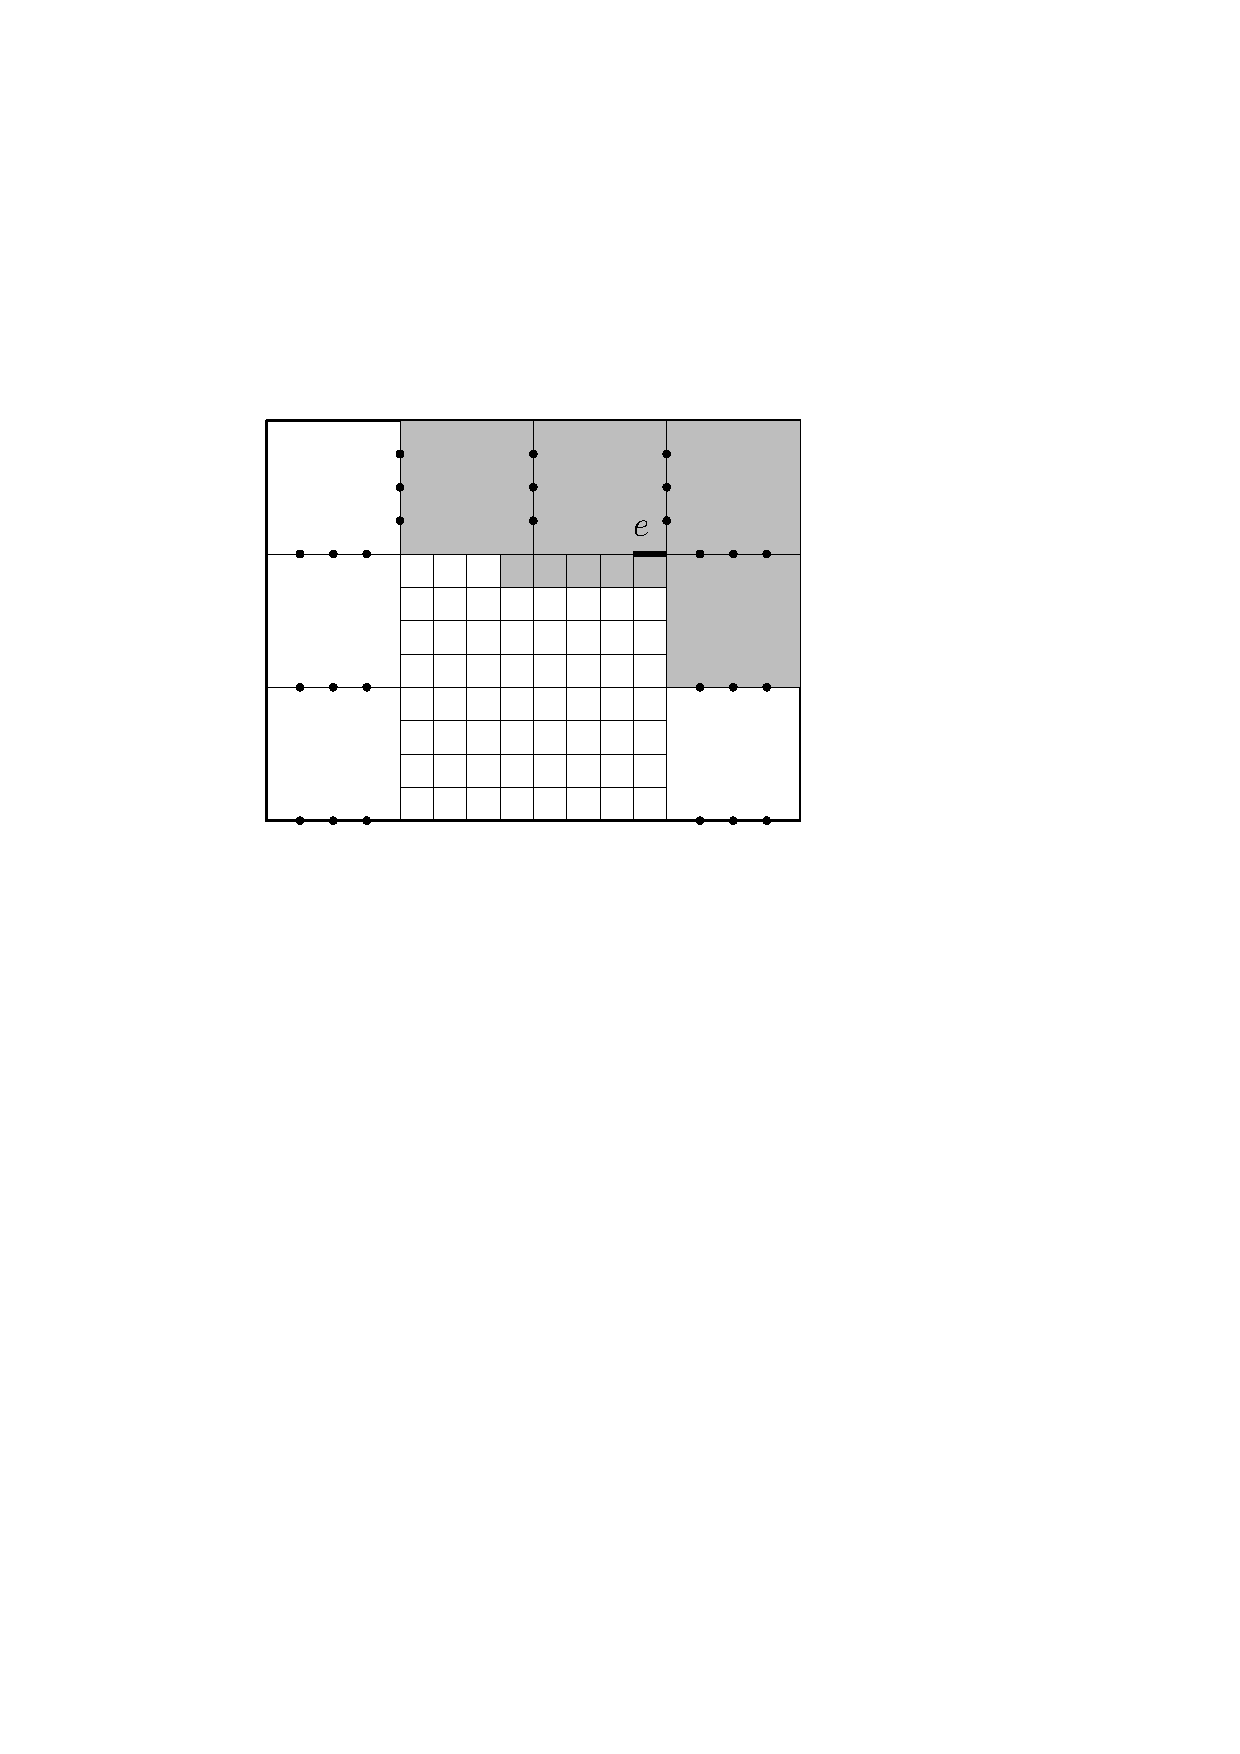
\includegraphics[width=0.5\textwidth]{figures/1conformingsubdivision.pdf}
	\caption{An example of part of an string 1-conforming subdivision. The shaded region 
    		 in the figure is the union of cell $\mathcal{U}(e)$ forming a well-covering 
             of edge $e$}
	\label{fig:1conformingsubdivision}
\end{figure}

As mentioned earlier in the overview of the Hershberger-Suri algorithm, the subdivision of 
$\mathcal{S}$ is similar to a quad-tree in that all its edges are horizontal or vertical. 
However, as we will see, the cells of $\mathcal{S}$ may not always be convex and the 
subdivision itself can be disconnected. As will shown later, each cell is still reasonably 
well-behaved, and there are at most one hole per cell. To give a more precise definition, 
each cell is either a square or a square-annulus.

\begin{mydef}
	\textbf{(Square-annulus:)}\\
	We will define it as a square $A$ which is missing  a square $B$ internally such that 
    the internal square $B$ is at least $1/4$ the side length of the outer square $B$
\end{mydef}

But the boundary of these cell may be subdivide into a constant number of edges.
We require also that they have the following minimum clearance property: 

\begin{mydef}
\textbf{(Minimum clearance property:)} \label{minimumclearanceproperty}\\
      The minimum width of an annulus in the subdivision (the minimum distance from the 
      inner square to the outer square) is at least one quarter of the side length of the 
      outer square. See Figure \ref{fig:minimumclearancesquareannulus}
\end{mydef}

\begin{figure}[H]
	\centering
	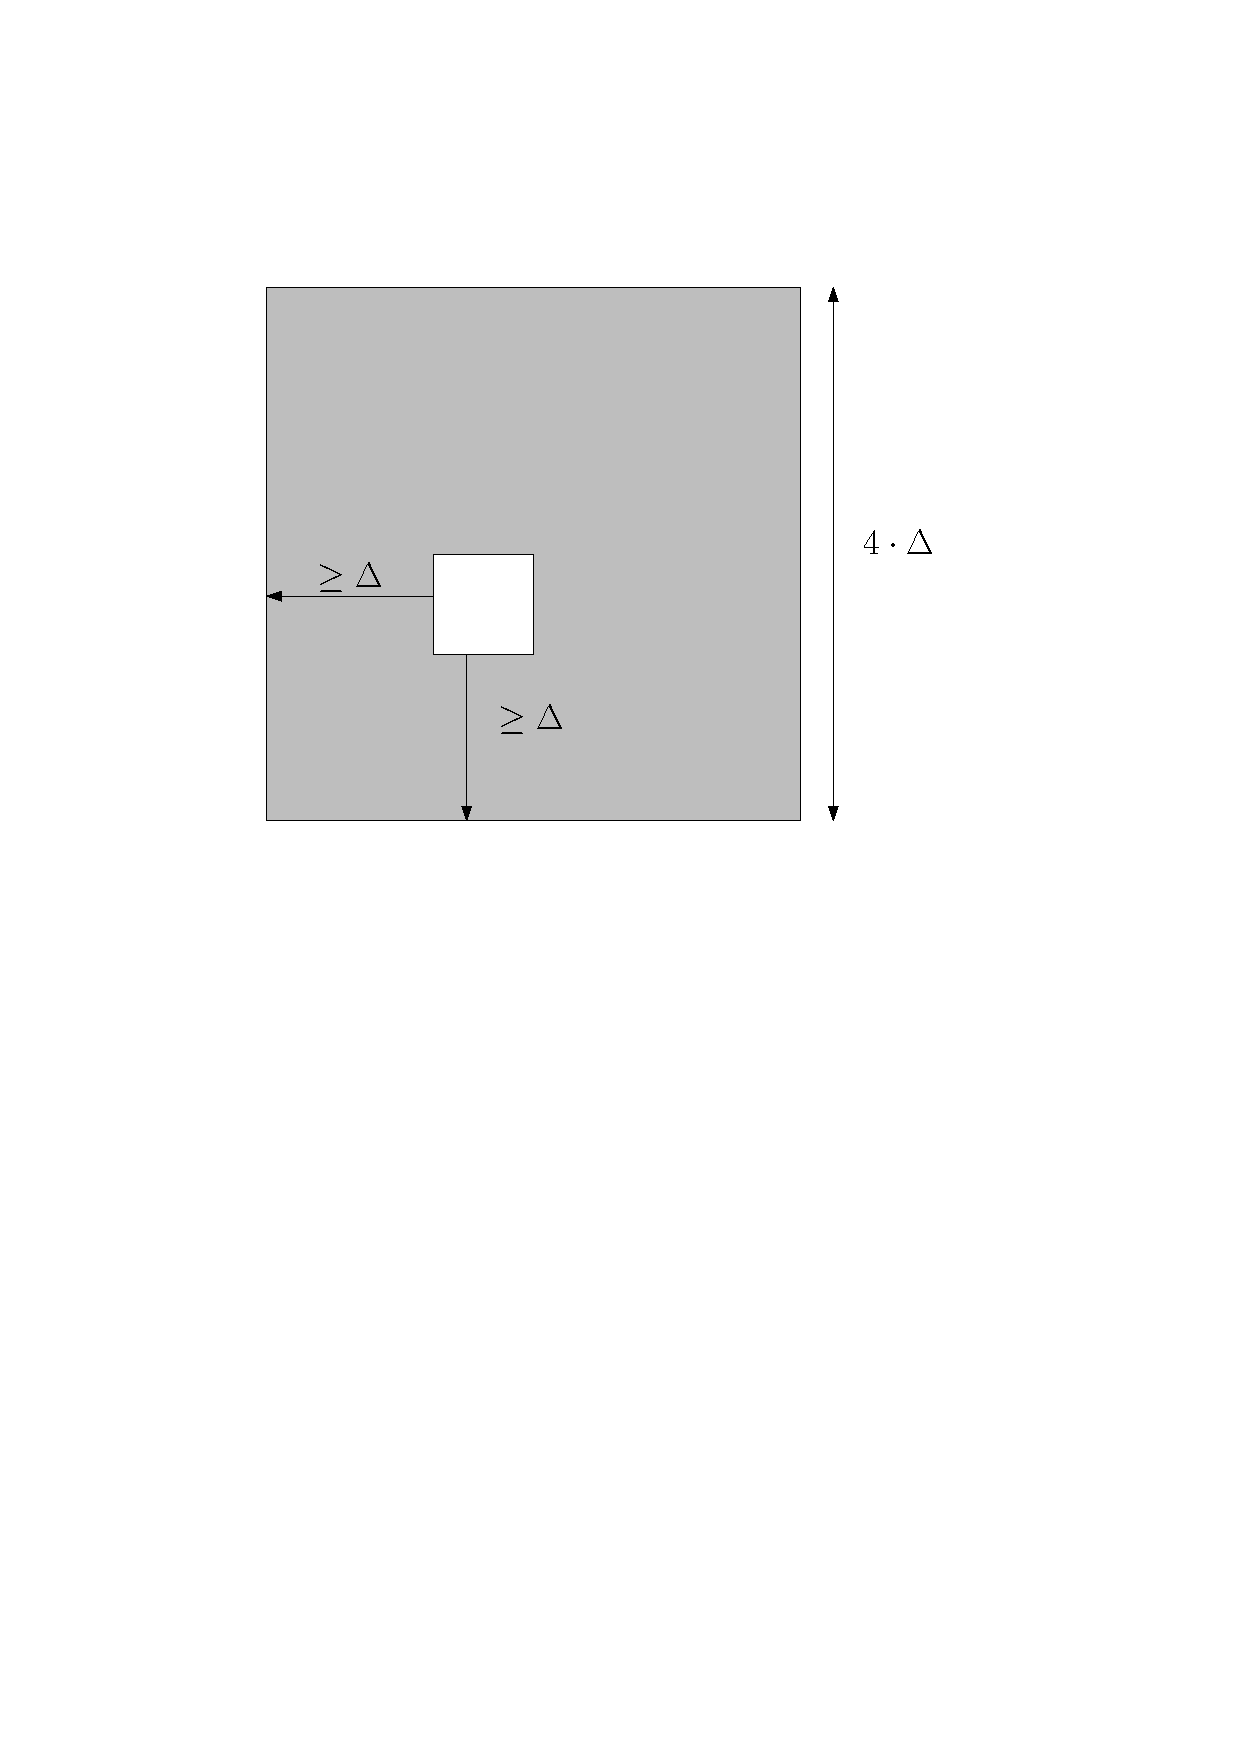
\includegraphics[width=0.5\textwidth]{figures/minimumclearance.pdf}
	\caption{A square-annulus, where the distance from the inner square to the outer 
  			 square, which is $\Delta$, is at least $1/4$ the side length of the outer 
             square which is $4\cdot \Delta$}
	\label{fig:minimumclearancesquareannulus}
\end{figure}

Both the annuli and square faces are subject to the uniform edge property:

\begin{mydef} \textbf{Uniform edge property:} 
\begin{itemize}
	\itemsep0em 
	\item Every edge on the outer square of an annulus has length
		  $1/(4\lceil \alpha \rceil)$ times the side length of the outer square.
	\item Every edge on the inner square has length $1/(4\lceil\alpha\rceil)$ times
		  the side length of the inner square.
	\item The lengths of edges on the boundary of a square cell differ by at
		  most a factor of 4.
\end{itemize}
\end{mydef}

\section{Conforming subdivision theorem}

The conforming subdivision theorem precisely states the properties we expect of our 
subdivision. It is also why this theorem will be proven by construction of the 
conforming subdivision algorithm which we will present in section 
\ref{section:implementationconforming}.

\begin{theorem}
	\label{theorem:conformingsubdivision}
	(Theorem 2.1 in \cite{HershbergerS99}) \textbf{Conforming Subdivision Theorem:} \\
	For any $\alpha\geq 1$, every set of $n$ points in the plane admits a strong
	$\alpha$-conforming subdivision of $O(\alpha n)$ size satisfying the
	following additional properties:
\begin{enumerate}	
	\item All edges of the subdivision are horizontal or vertical,
	\item Each face is either a square of a square-annulus, with subdivided
		boundary,
	\item Each annulus has the minimum clearance property,
	\item Each face has the uniform edge property, and
	\item Every data point is contained in the interior of a square face
\end{enumerate}
	Such a subdivision can be computed in time $O(\alpha n + n\log n)$.
\end{theorem}

This theorem implies that we need to make modifications to the strong conforming 
subdivision of $V$ to accommodate for the edges of the obstacles, because our goal is 
to produce a \textit{conforming subdivision of the free space}. This is done by 
modifying the edges present in the subdivision, s.t. we differentiate between the edges 
introduced by the subdivision construction and the edges of obstacles. We mentioned the 
difference between these before, but for completeness we here present a formal 
definition of these differences.

\begin{mydef}\textbf{Transparent and opaque edges:}\\
    Let the edges in a conforming subdivision of the free space, which are introduced by 
    the subdivision be transparent edges. Equally let the edges in a conforming 
    subdivision of the free space, which are introduced by the original obstacles be 
    opaque edges. 
\end{mydef}

The reason, as mentioned before, we the need to differentiate between these, is due to the 
fact that the algorithm allows wavefronts to pass through transparent edges, but are blocked 
by the opaque edges. We also require that the transparent edges are well-covered in the 
conforming subdivision of the free space, even though they don't need to be strongly 
covered. Due to these requirement, we will slightly alter definition 
\ref{def:wellcoveringwithpara} first and third requirement as such:

\begin{enumerate}
\item[W1$_{fs}$.] Let $e$ be a tranparent edge of $\mathcal{S}$. There exists a set of 
cells $\mathcal{C}(e)\subseteq\mathcal{S}$ such that $e$ is contained in the closure 
of the uinion of cells $\mathcal{U}(e)=\{c|c\in\mathcal{C}(e)\}$.
\item[W3${fs}$.] Let $e$ and $f$ be two transparent edges of $s$ such that $f$ lies on 
the boundary of the well-covering region $\mathcal{U}(e)$. Then the shortest path 
distance between $e$ and $f$ is at least $\alpha\cdot\max(|e|,|f|)$. 
\end{enumerate}

It is worth noting that condition $3_{fs}.$ ensures $e$ does not touch any transparent 
boundary edge of $\mathcal{U}(e)$, although it may touch opaque boundary edges.

\section{Construction of the conforming subdivision}

In this section we go through the basic building blocks used for computing the conforming 
subdivision, $i$-boxes and $i$-quads, and some nice properties and behavior of them. We will go 
through the overlap relation, which is used to make set of equivalence classes of $i$-quads. These 
equivalence classes are the main component for the two algorithms which will calculate the conforming 
subdivision. We will also briefly show a lemma for transforming a $1$-conforming subdivision to a 
$\alpha$-conforming subdivision, for a constant $\alpha$. Finally we will discuss the invariants of 
the of the conforming subdivision algorithms, before moving on to discuss the algorithm in the next 
section. 

\subsection{Definitions of $i$-boxes and $i$-quads}

Before going into the algorithm for constructing the conforming subdivision, wee need
preliminary terminology and definitions.

To make things easy for our selfs, we fix a Cartesian coordinate system in the plane we are 
working with. We say for any integer $i$ and $k$, the $i$'th-order grid in the coordinate 
system is the arrangement of all lines $z = k \cdot 2^i$ and $y = k \cdot 2^i$. This makes a 
grid where each cell (face), is a square of size $2^i \times 2 ^i$, whose lower-left corner 
lies at the point $(k \cdot 2^i, l \cdot 2^i)$, for any pair of integers $k$ and $l$. We will 
refer to such a cell as an $i$-box. Any array of size $4 \times 4$ is called an \textit{i-
quad}, see figure \ref{fig:iquad}.

\begin{figure}[H]
	\centering
	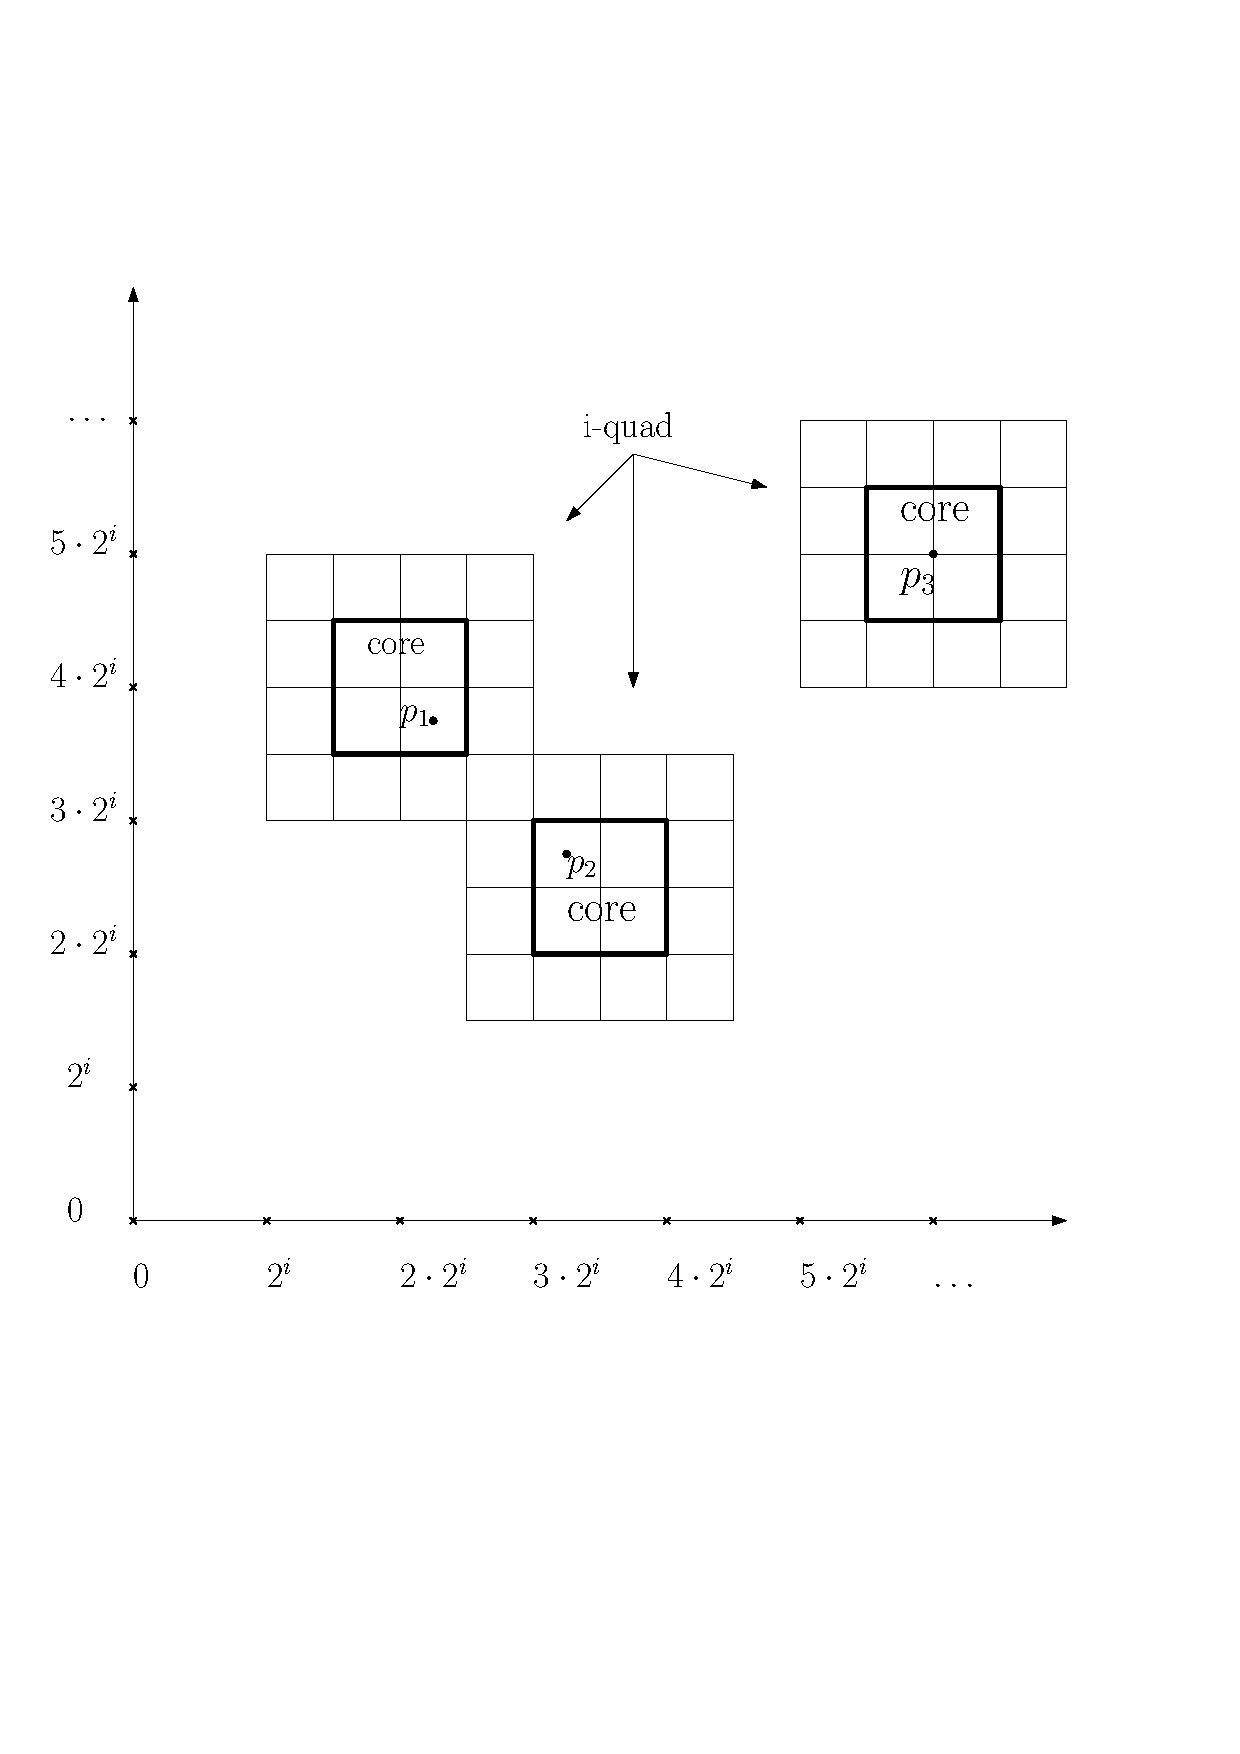
\includegraphics[width=0.7\textwidth]{figures/iquad.pdf}
	\caption{The figure show an example of how i-quads would be grown around the point $p_1, 
    		 p_2$ and $p_3$. Here we also see that in this particular $i$'th stage of growth, 
             that $p_1$ and $p_3$ belong to the same equivalence class, while $p_3$ does 
             not.}
	\label{fig:iquad}
\end{figure}

One could note that, while it is true that the size of an $i$-quad is the same as an 
$(i+2)$-box, an $(i+2)$-box may not be a cell in the $(i+2)$-order grid. So these are not 
always equal. We also refer to the four non-boundary $i$-boxes of an $i$-quad as the core of 
the $i$-quad, see figure \ref{fig:iquad}. By this definition the core is always an $2 \times 
2$ array in the $i$-boxes. One can also observe that an $i$-box $b$ may have up to four 
$i$-quads that contain $b$ in their cores.

The algorithm for building a $1$-conforming subdivision, is in a quad-tree-like fashion where 
we build a partition around the set of points in the plane in a bottomup procedure. This i done 
by \textit{growing} a square box around each data point, until the entire plane is covered by 
these boxes. This is done in a number of discrete \textit{stages} numbered $-2, 0, 2, 4,...$. 
The end goal is to produce a $1$-conforming partition of the points, where the subdivision will 
be a grid with orthogonal cells. Key idea behind the growth process is, each data point $p$ in
stage $i$ is in the core of an $i$-quad. And since we grow the initial box, the data point $p$
will remain in the $i$-quads core, and the following lemma holds inductively, by definition of
the process we have described.

\begin{Lemma}
Each $(i-2)$-quad constructed in stage $(i-2)$ lies in the core of some $i$-quad constructed in 
stage $i$. 
\end{Lemma}

To lower overhead of the algorithm, we only maintain a minimal set of quads at any given $i$-stage.
We denote the set of quads in stage $i$ with $\mathcal{Q}(i)$. This set is partitioned into 
equivalence classes under the transitive closure of an \textit{overlap} relation. 

\begin{mydef} \textbf{(Overlap relation:)} \\
Given any two quads $q$ and $q'$, we say these are in the same equivalence class, by the overlap 
relation, if and only if there is a sequence of quads $q = q_0, q_1, ..., q_m = q' \in 
\mathcal{Q}(i)$, s.t. $q_j$ and $q_{j+1}$ overlap (have common interior point) for all $j = 0, 1, 
..., m - 1$. Further more, let $\{S_1(i), ..., S_k(i)\}$ denote the partition of $\mathcal{Q}(i)$ 
into these equivalence classes in the $i$th stage, and let $\equiv_i$ denote the transitive 
equivalence relation. 
\end{mydef}

We denote a region, or to be more exact the partition of the plane, covered by the quads of one 
class a \textit{component}. By previous definitions we know that a component in stage $i$ either 
is a single $i$-quad, of the a union of $i$-quads where the points in each $i$-quads core, belong 
to the same equivalence class. We differentiate between two types of classes. The first being a 
\textit{simple} component. A component at stage $i$ is simple if

\begin{enumerate}
\item Its outer boundary is an $i$-quad and
\item It contains exactly on $(i-2)$-quad of $\mathcal{Q}(i-2)$ in its interior.
\end{enumerate}

The second type is a complex component. A complex component is complex if it is not simple.

\subsection{Merging of $i$-quad} \label{section:mergingiquad}

In this subsection we show some distance properties that is satisfied by points of the same 
equivalence class at stage $i$, which will be useful in the final algorithm. We say that a quad 
$q$ is a \textit{containing $i$-quad} of a point $u \in V$ if $q \in \mathcal{Q}(i)$ and $u$ lies 
in $q$'s core. We also say that a point $u$ \textit{belongs} to an equivalence class $S \in 
\mathcal{Q}(i)$ if there is a containing $i$-quad of $u$ in $S$.

\begin{Lemma} (Lemma 6.6 in \cite{HershbergerS99}) \label{lemma:6.6HershbergerS99}\\
Let $u$ be a point of $V$ and let $q \in \mathcal{Q}(i)$ be a containing $i$-quad of $u$. Then 
the minimum distance between $u$ and the outer boundary of $q$ is $2^i$.
\end{Lemma}

\begin{proof}
The key idea is the property that $u$ lies in the core of $q$, which we know the size of. Since 
$q$ has side length $2^{i+2}$, and $u$ lies at least a quarter of this distance away from the 
outer boundary, the lemma trivially follows.
\end{proof}

As used earlier in the thesis, we use the notation $d(u,v)$ to denote the distance between the 
points $u$ and $v$.

\begin{Lemma} (Lemma 6.7 in \cite{HershbergerS99}) \label{lemma:6.7HershbergerS99} \\
Let $u$ and $v$ be two points of in the plane that belong to two different equivalence classes of 
$\mathcal{Q}(i)$. Then $d(u,v) > 2 \times 2^i$.
\end{Lemma}

\begin{proof}
Let $q_u$ and $q_v$ be two containing $i$-quads for $u$ and $v$, respectively. Since $u$ and $v$ 
lie in different equivalence classes, these $i$-quads cannot intersect. By Lemma 
\ref{lemma:6.6HershbergerS99}, each of the points lies at least a distance $2^i$ away from 
the outer boundaries of their $i$-quads, which immediately gives a lower bound of $d(u,v) > 2 
\times 2^i$, which proofs the lemma.
\end{proof}

\begin{Lemma} (Lemma 6.8 in \cite{HershbergerS99}) \label{lemma:6.8HershbergerS99}\\
Let $u$ and $v$ be two points in the plane and let $q_u$ and $q_v$, respectively, be the two $i$-quads of $\mathcal{Q}(i)$ containing them. If $q_u \cap q_v \neq \emptyset$, then $d(u,v) < 6 
\times 2^i$.
\end{Lemma}

\begin{proof}
By Lemma \ref{lemma:6.6HershbergerS99}, the maximum distance between $u$ and the outer boundary 
of $q_u$ is at most $3 \times 2^i$. The same holds for $v$ and $q_v$, which implies the upper 
boundary of $d(u,v) < 6 \times 2^i$. See figure \ref{fig:lessthan6i}.
\end{proof}

\begin{figure}[H]
	\centering
	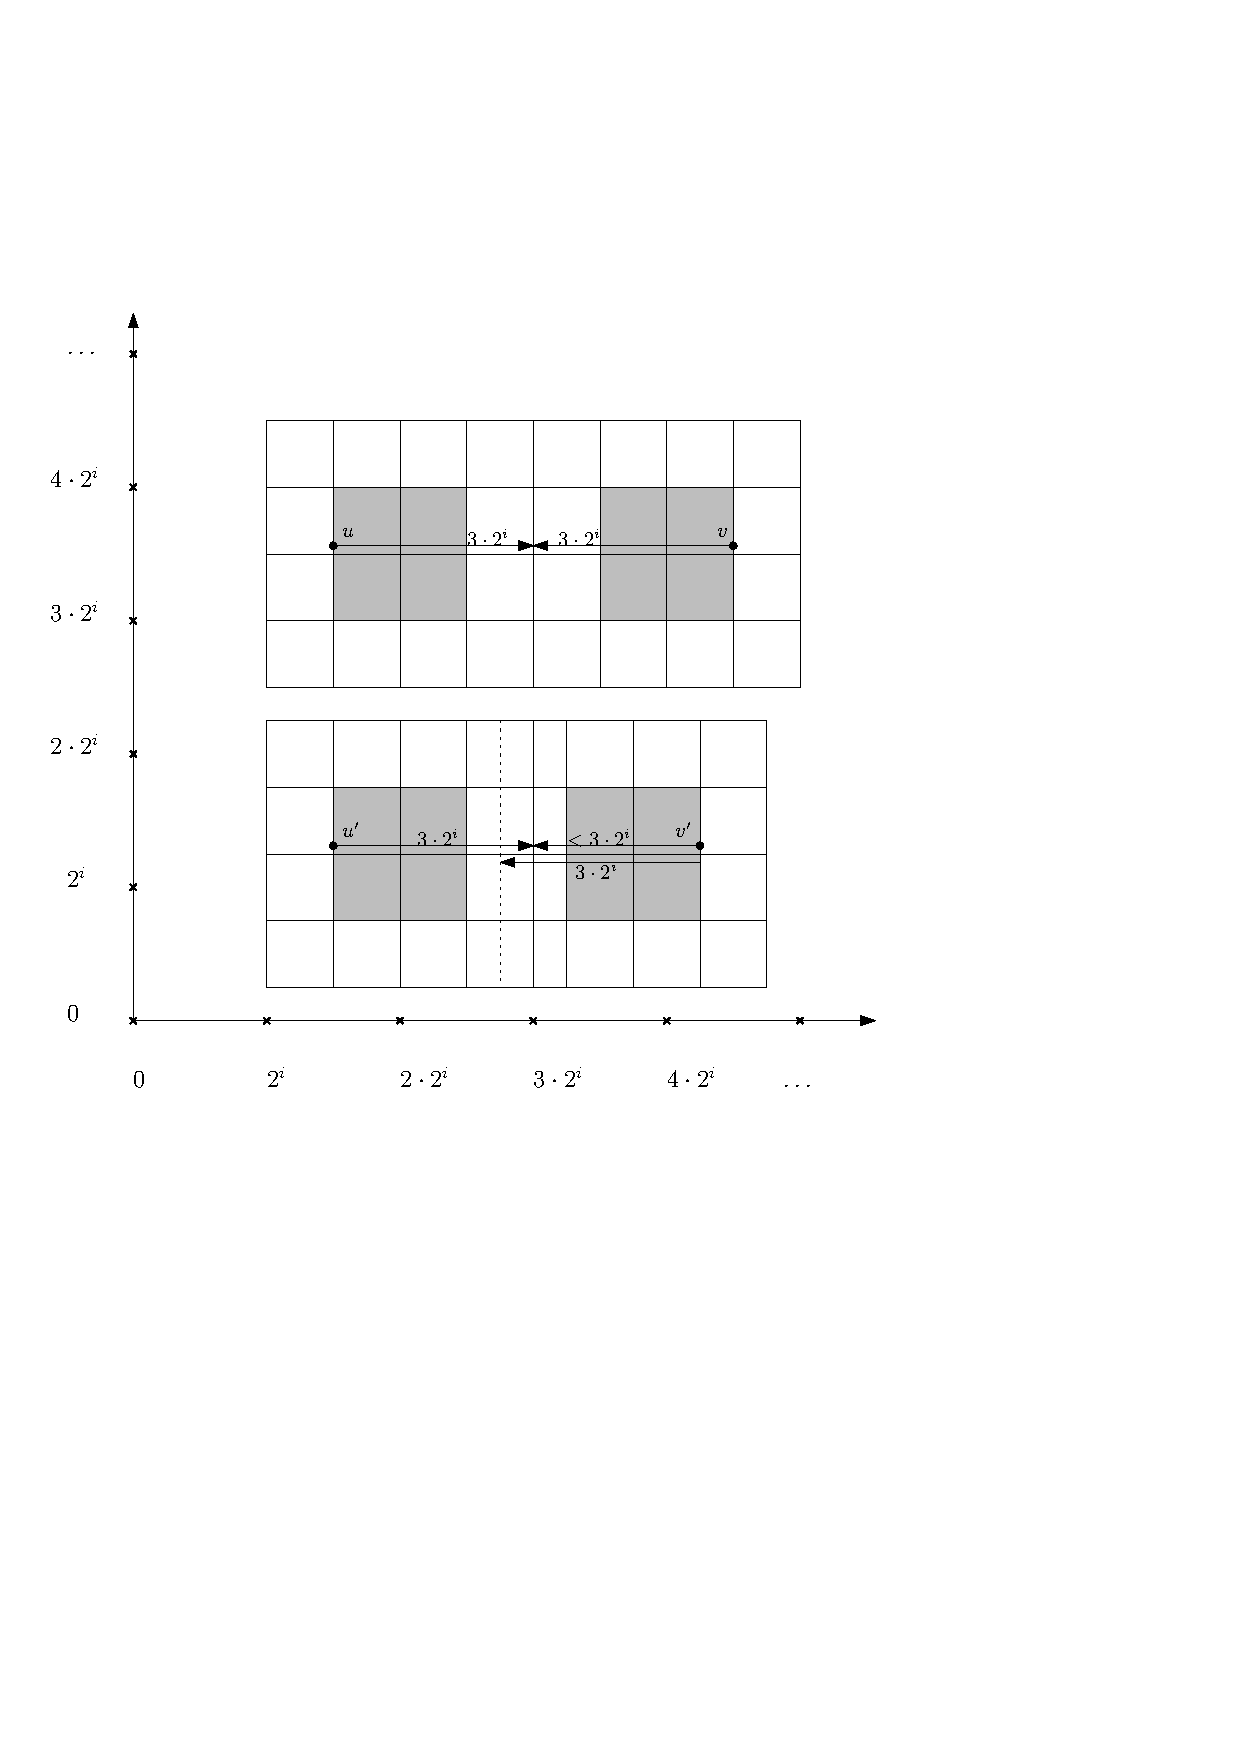
\includegraphics[width=\textwidth]{figures/lessthan6i.pdf}
	\caption{The two top $i$-quads with points $u$ and $v$ are as close as they can be without 
    		 belonging to the same equivalence class, that is not overlapping, and therefore have 
             $d(u,v) = 6 \times 2^i$. The two lower $i$-quads with points $u'$ and $v'$ overlap, and 
             therefore have $d(u,v) < 6 \times 2^i$.}
	\label{fig:lessthan6i}
\end{figure}

\subsection{Transforming $1$-conforming subdivision to $\alpha$-conforming subdivision}

The following lemma shows how to transform a $1$-conforming subdivision into an $\alpha$-conforming 
subdivision of size $O(\alpha\cdot n$ in $O(\alpha\cdot n)$ time. This is quite important for the 
correctness of our algorithm, since we will need the ability to transform the $1$-conforming 
subdivision to an $\alpha$-conforming subdivision.

\begin{Lemma} (Lemma 6.1 from \cite{HershbergerS99}) \label{lemma:6.1HershbergerS99} \\
Let $V$ be a set of $n$ points, and let $\mathcal{S}_1$ be a $1$-conforming 
subdivision for $V$ of size $O(n)$. For any $\alpha>1$, we can build an $\alpha$-conforming 
subdivision $\mathcal{S}_\alpha$ for $V$ with complexity
\end{Lemma}

\begin{proof} Subdivide each edge of $\mathcal{S}_1$ into $\lceil \alpha
	\rceil$ equal-length pieces. Define the well-covering region of each edge
	$e$ in $\mathcal{S}_\alpha$ to be the same as the well-covering region in
	$\mathcal{S}_1$ of which $e$ is a fragment. These operations can performed
	in $O(\alpha\cdot n)$ time. 

We show below that the subdivision thus defined satisfies properties from
	definition \ref{def:aconformingsubdivision}. 

\begin{enumerate}
    \item $\mathcal{S}_\alpha$ has the same set of cells as $\mathcal{S}_1$, so each cell of 
    	  $\mathcal{S}_\alpha$ contains at most one point of $V$ in its closure.
    \item Each internal edge $e_\alpha$ of $\mathcal{S}_\alpha$ is well-covered with 
    	  parameter $\alpha$, since it satisfies the conditions stated in 
          \ref{def:wellcoveringwithpara}. Let $e_1$ be the edge of $\mathcal{S}_1$ of which 
          $e_\alpha$ is a fragment. Let $C_\alpha(e_\alpha)$ be the set of cells of 
          $\mathcal{S}_\alpha$ whose union $\mathcal{U}_\alpha(e_\alpha)$ is the well-
          covering region of $e_\alpha$. Define $\mathcal{C}_1(e_1)$ and $\mathcal{U}(e_1)$ 
          analogously.
    \begin{enumerate}
    	\item $\mathcal{U}_\alpha(e_\alpha)$ covers the same area as $\mathcal{U}_1(e_1)$, 
        	  so $e_\alpha$ is contained in its interior.
        \item Each edge of each cell in $\mathcal{C}_1(e_1)$ is divided in $\lceil \alpha 
        	  \rceil$ pieces in $\mathcal{C}_\alpha(e_\alpha)$ is $O(\alpha)$.
        \item Let $f_\alpha$ be an edge of $\mathcal{S}_\alpha$ on (or outside in the case 
        	  of strongly 1-conforming) the boundary of $\mathcal{U}_\alpha(e_\alpha)$, and 
              let $f_1$ be the edge of $\mathcal{S}_1$ from which it is derived. The 
              Euclidean distance between $e_\alpha$ and $f_\alpha$ is at least as large as 
              the distance between $e_1$ and $f_1$, which is at least $\max(|e_1|,|f_1|)\geq 
              \max(\alpha\cdot|e_\alpha|, \alpha\cdot|f_\alpha|)$.
    \end{enumerate}
    \item Well-covering regions in $\mathcal{S}_\alpha$ are the same as in $\mathcal{S}_1$, 
    	  so each contains at most one vertex of $V$.
\end{enumerate}
Which establishes the lemma.
\end{proof}

\subsection{The invariants}

The main objective of the algorithm is to draw the boundaries of certain components, which in 
the end will give the correct subdivision. Each of these edges will be straight line segments,
all parallel to one the axes, and will be subdividing the plane into orthogonal cells. The 
critical property of our subdivision is the following \textit{conforming property:}

\paragraph{Invariant 1:} For any edge $e$ and cell $c$ of the subdivision, $c$ has an interior 
point within distance $|e|$ of $e$ if and only if $c$ and $e$ are incident (their closures 
intersect). Thus There are at most six cells within distance $|e|$ of any edge $e$. \\

The algorithm will only draw edges of increasing lengths, and so we never need to subdivide 
previously drawn edges inside a component. In order to maintain Invariant 1, the algorithm 
will also enforce the following auxiliary invariant:

\paragraph{Invariant 2:} The boundary of each complex component in stage $i$ is subdivided 
into edges of length $2^i$ that are aligned with the $i$th-order grid\footnote{both invariants 
are as defined in \cite{HershbergerS99} section 6.2}. \\

Through the algorithm the outer boundary of simple components, wont be drawn until just before 
they merge with other components to form complex components. This will show itself very valuable,
since this helps to ensure the upper bound of the size for the final subdivision of $O(n)$.

The algorithm consists of two main sub-algorithms. The first procedure \textit{\textbf{growth}}, 
will take care of simulating the growth of the $(i-2)$-quads to $i$-quads at a stage $i$. The 
second procedure \textit{\textbf{build-subdivision}}, will compute and maintain the equivalence 
classes, and will also draw the subdivision edges (which will satisfy invariant 1 and 2). 

First we will present \textbf{build-subdivision}, and then move on to presenting \textbf{growth}. 
All we need to know about \textbf{growth} for now is, given an $i$-quad $q$, the procedure 
$\mathbf{growth}(q)$ will produce a $(i+2)$-quad containing $q$ inside its core. For a family 
$S$ of $i$-quads, $\mathbf{growth}(S)$ is a minimal set of $(i+2)$-quads satisfying the following:

$$\forall q \in S, \quad \exists \bar{q} \in \mathbf{growth}(S) \quad \text{s.t.} \quad \bar{q} 
= \mathbf{growth}(q)$$

As mentioned earlier, up to four $(i+2)$-quads may contain the $i$-quad $q$ in their cores. So 
to not complicate matter, we will postpone the discussion of how the procedure \textbf{growth} 
chooses $\mathbf{growth}(q)$. For now we will be content with $\mathbf{growth}(q)$ being a 
unique $(i+2)$-quad returned by the procedure \textbf{growth}. We also use the notation $\bar{q}$ 
to denote $\mathbf{growth}(q)$.

\section{Pseudo Code for \textbf{build-subdivision}}

To assure that all components will be simple and disjoint at the initial state, and not complex 
(overlap) we will scale the plane in such a way that either the horizontal or the vertical 
distance between any two points in the plane is at least 1, and no points has a coordinate which 
is a multiple of $1/4$. We compute a $(-2)$-quad for every point $p$ in the plane, with $p$ in 
the upper left corner of the $(-2)$-boxes core. These quads form the initial set of quads in 
$\mathcal{Q}(-2)$. Since no $i$-quad overlaps, they all belong to their own equivalence class, 
and can in this context be regarded as singletons. We proceed to draw the $(-2)$-box around 
each point $p$, which will be contained in the core of the $(-2)$-box, which we won't draw now. 
From this initial setup, one can easily see that the invariants are satisfied, and we are ready 
to proceed with the \textbf{build-subdivision} algorithm:

\begin{algorithm}[H]
	\caption{Algorithm \textbf{build-subdivision}} \label{algorithm:build-subdivision} 
	\begin{algorithmic}[1]
		\While {$|\mathcal{Q}(i)| > 1$} 
        	\State $i = i + 2$
			\State Initialize $\mathcal{Q}(i)=\emptyset$
            \ForEach {equivalence class $S$ of $\mathcal{Q}(i-2)$}
            	\State $\mathcal{Q}(i)=\mathcal{Q}(i)\cup\mathbf{growth}(S)$.
            \EndFor
            \ForEach {pair of $i$-quads $q,q'\in\mathcal{Q}(i-2)$}
            	\If {$q \cap q' \neq \emptyset$}
                	\State Set $q \equiv_i q'$.
                \EndIf
            \EndFor
            \State \multiline{Extend $\equiv_i$ to an equivalence relation by transitive closure, 
            				  and compute the equivalence class}
    		\ForEach {$q\in \mathcal{Q}(i-2)$}
            	\State Let $\bar{q} = \mathbf{growth}(q)$ as computed in step $2-8$
                \If {$q$ is a simple component of $\mathcal{Q}(i-2)$ 
						 but $\bar{q}$ isn't a simple component of
						 $\mathcal{Q}(i)$(*)}
                     \State \multiline{Draw the boundary box of $q$ and subdivide each of its
                     		sides into four edges at the $(i-2)$-order grid lines.}
                \EndIf
            \EndFor
            \ForEach {equivalence class $S$ of $\mathcal{Q}(i)$}
                \State Let $S'=\{q\in\mathcal{Q}(i-2) \quad s.t. \quad 
                	   \mathbf{growth}(s)\in S\}$.
                	\If {$|S|>1$}
                        \State Let $R_1 = \cup_{q\in S'} \{$the core of 
                        	   \textbf{growth}$(q)\}.$
                        \State Let $R_2 = \cup_{q\in S'} \{$the region covered by 
                        	   $q\}.$
                        \State \multiline{Draw $(i-2)$-boxes to fill the region between the 
                        	   boundaries of $R_1$ and $R_2$.}
                        \State \multiline{Draw $i$-boxes to fill the region between the 
                        	   boundaries of $R_1$ and $S$; break each cell boundary 
                               with an endpoint incident to $R_1$ into four edges of 
                               length $2^{i-2}$, to satisfy Invariant 1.}
                    \EndIf
            \EndFor
		\EndWhile
	\end{algorithmic} 
\end{algorithm}
(*)\peter{HOW TO FIX!?}
As we explained earlier, the algorithm runs in discrete stages of $-2, 0, 2, 4, ... $, which we 
see in the increment step of step 2. Step 3 to step 8 computes the $\mathcal{Q}(i)$ from 
$\mathcal{Q}(i-2)$. This is done by growing the previous squares from $\mathcal{Q}(i-2)$, one 
equivalence class at a time, and the see if any of the newly grown squares overlap. If this is 
the case, the belong to the same equivalence class, and should be marked as suck in 
$\mathcal{Q}(i)$. Next in step 10 to 13 we process the simple components of $\equiv_{i-2}$ that 
are about the merge with other components. This is done by checking if the square $q$ which was 
simple before the growth process still would be simple after the growth. If not we draw the 
boundary box of $q$ before the growth, and subdivide its sides into edges of equal length, each 
a quarter of the total side length. The last steps 14 to 20 are dedicated to processing the 
complex components. Here we compute a $S'$ which consists of the $q \in \mathcal{Q}(i-2)$ which 
will grow into the equivalence class $S$ in $\mathcal{Q}(i)$. We will only process if $|S'| > 1$ 
which means $S$ would be complex. Here create two set $R_1$ being the cores of the $i$-quads in 
the complex equivalence class $S$ and $R_2$ being the region covered by the $q$ in $S'$. Should 
these not overlap we fill the region between $R_1$'s and $R_2$'s boundaries with $(i-2)$-boxes. 
In the last step we basically draw the outer boundaries of the $growth(q)$ square, to fill the 
space between the cores, $R_1$, and the outer boundary of $S$, with edges that satisfy our 
invariant. 

This is the overall idea behind the \textbf{build-subdivision} algorithm. This pseudo code, 
while not being efficient enough, gives a good understanding of what we want it to do. We will 
visit this algorithm again in section \ref{section:implementationconforming}, at improve it to 
an $O(n \log n)$ implementation, the needed supporting data structures and more.

\section{Pseudo Code for \textbf{growth}}

The overall idea behind the algorithm for \textbf{growth($S$)} is to build a graph on the quads 
in $S$. 

\begin{algorithm}[H]
	\caption{Algorithm $\mathbf{growth}(S)$} 
	\begin{algorithmic}[1]
		\State Set $\mathbf{growth}(S)=\emptyset$
        \ForEach {pair of quads $q_1,q_2\in S$}
        	\If {$q_1 \cup q_2$ can be contained in a $2 \times 2$ array of $(i+2)$-boxes}
                \State Put an edge between $q_1$ and $q_2$.
            \EndIf
        \EndFor
        \State Compute a maximal matching in the graph computed in Step 1
        \ForEach {edge $(q_1, q_2)$ in the maximal matching}
        	\State Choose an $(i+2)$-quad $\bar{q}$ containing $q_1, q_2$ in its core.
            \State Set $\mathbf{growth}(q_1)=\mathbf{growth}(q_2)=\bar{q}$, and add 
            	   $\bar{q}$ to $\mathbf{growth}(S)$.
        \EndFor
        \ForEach {unmatched quad $q\in S$}
        	\State Set $\mathbf{growth}(q)=\bar{q}$, where $\bar{q}$ is an $(i+2)$-quad 
            	   containing $q$ in its core.
            \State Add $\bar{q}$ to $\mathbf{growth}(S)$.
        \EndFor
	\end{algorithmic} 
\end{algorithm}

Initially we set $\mathbf{growth}(S)$ to be empty. Step 2 to step 4 builds a graph whose 
nodes are the $i$-quads of $S$, with the property that their collective area can be contained 
in a grid of $2 \times 2$ $(i+2)$-boxes. If this is the case we connect the two nodes. In step 
5 we compute a maximal matching of the graph.

\begin{mydef} {Maximal matching} \\
Given a graph $G = (V,E)$, we define a matching $M$ in $G$ to be the set of pairwise 
\textit{non-adjacent} edges; that is, no two edges will have a vertex in common. A maximal 
matching is then defined as a matching $M$ of $G$ with the property that if any edge not in 
$M$ is added to $M$, then $M$ will no longer be a matching. By this definition, we see that 
a maximal matching $M$ is a superset of all other matchings of $G$, where further $M$ can't 
be a subset of the other matching of $G$. See figure \ref{fig:imperfectmatching} and 
\ref{fig:perfectmatching} \peter{wikipedia}
\end{mydef}

\begin{figure}[H]
	\centering
	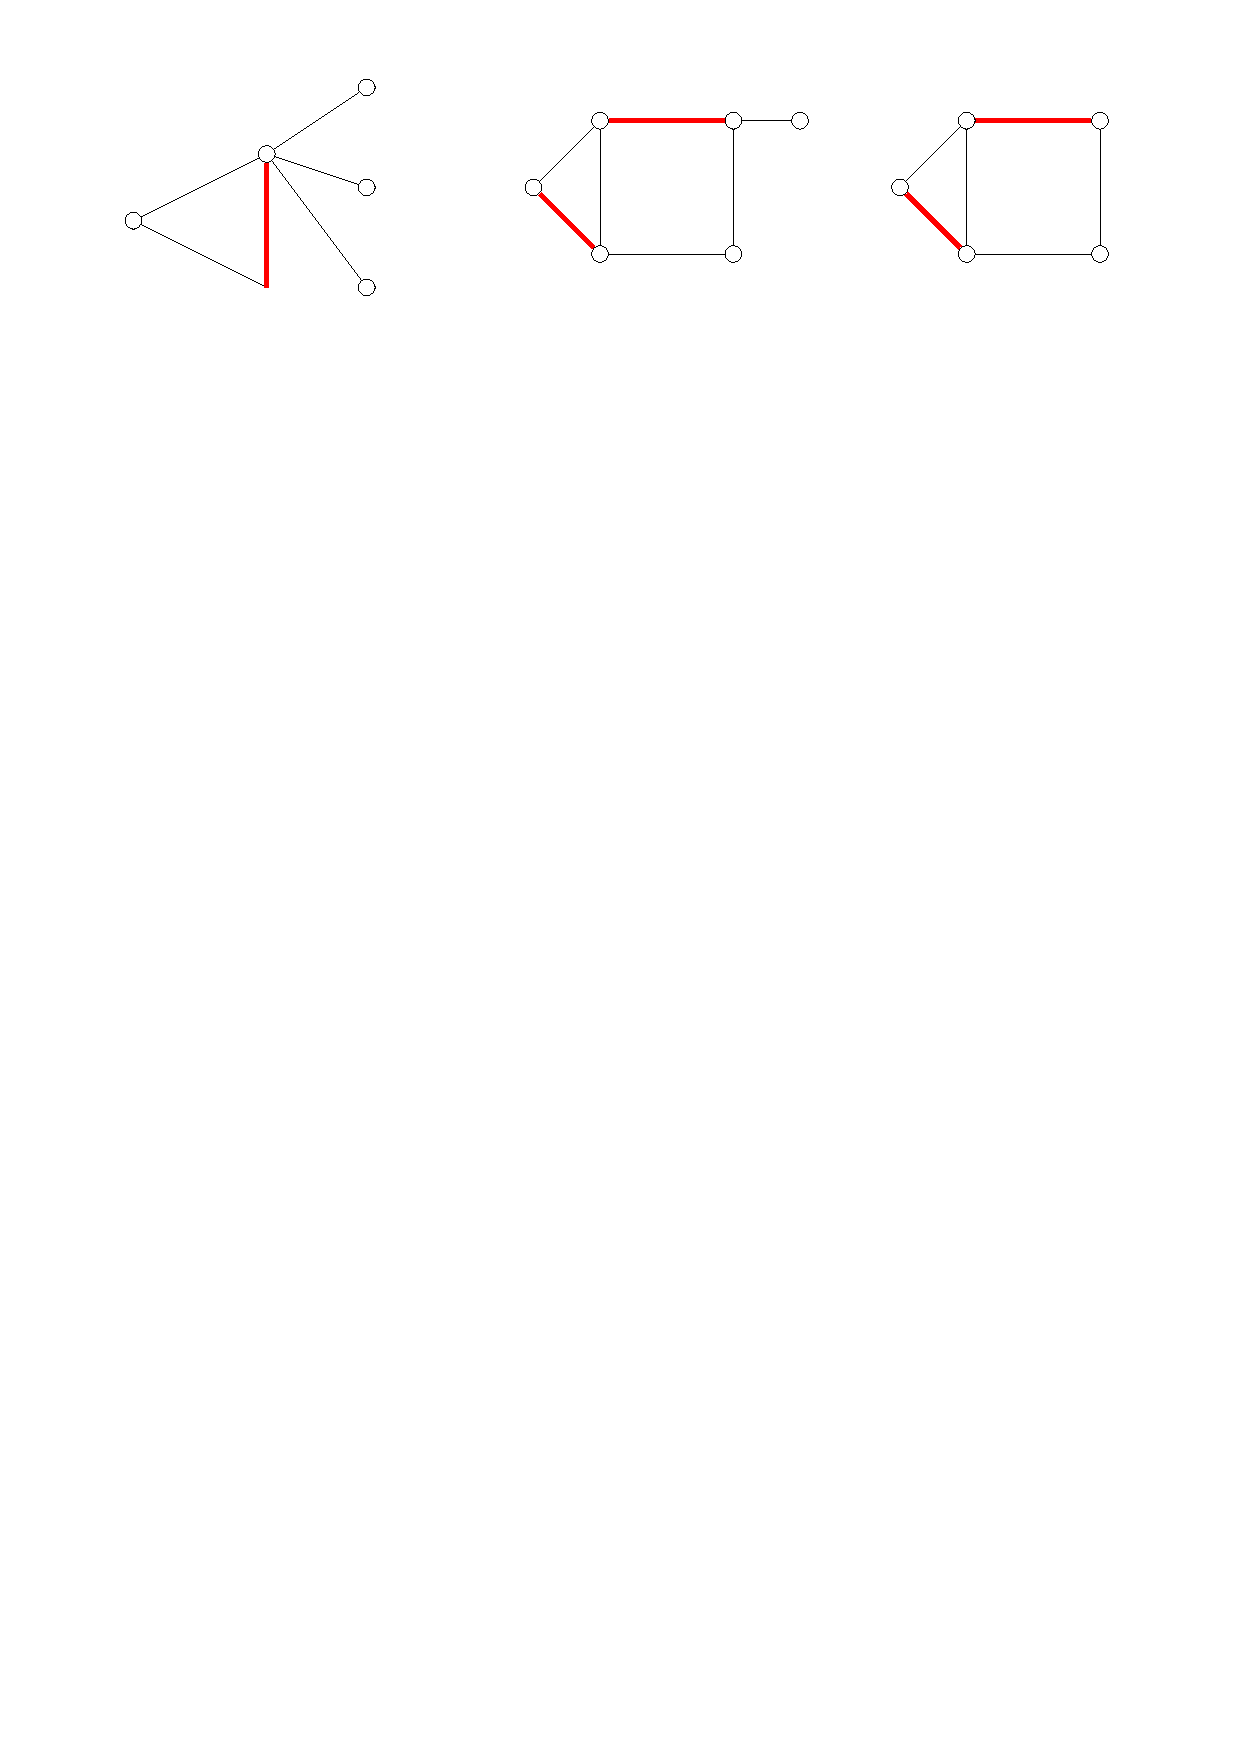
\includegraphics[width=0.7\textwidth]{figures/imperfectmatching.pdf}
	\caption{The figure shows three examples of non maximal matching}
	\label{fig:imperfectmatching}
\end{figure}

\begin{figure}[H]
	\centering
	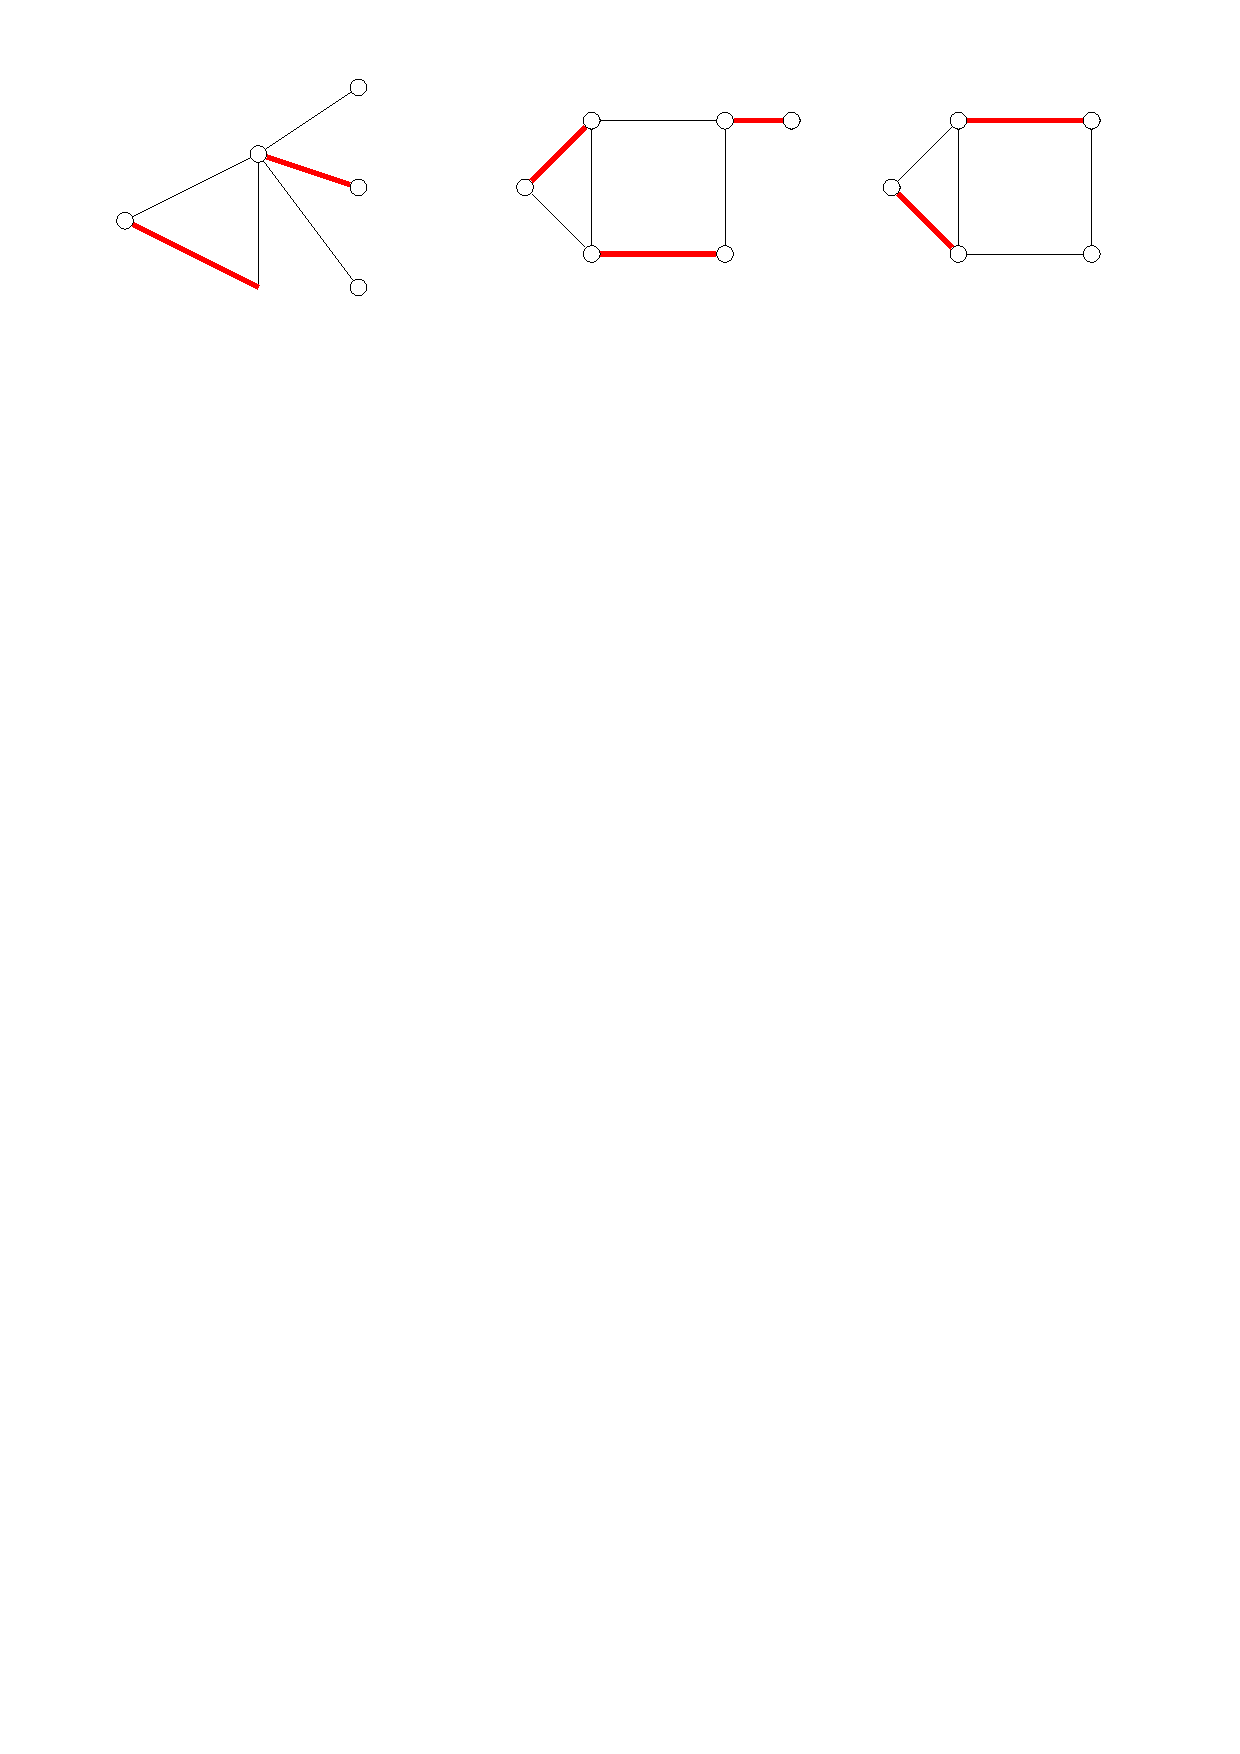
\includegraphics[width=0.7\textwidth]{figures/perfectmatching.pdf}
	\caption{The figure shows three examples of maximal matching, one should notice that the last 
    		 figure have multiple maximum matching, each with two edges.}
	\label{fig:perfectmatching}
\end{figure}

We will save the proof of correctness of the \textbf{growth} algorithm for section 
\ref{section:correctnessgrowth}, but it is worth noting that the maximum node degree of the 
graph build in step 2 to 4, is of constant since, $O(1)$. This is due to the fact that only a 
constant number of $i$-quads can touch any $i$-quad $q$. This implies the maximal matching in 
this graph has $\Theta (|E|)$ edges. Since \textbf{growth} basically maps an $i$-quad to its 
larger counter part in the next stage, each $i$-quad at stage $i$ maps to an $(i+2)$-quad in 
stage $(i+2)$. And since each matching edge, that is the edges marked in step 5, corresponds 
to two $i$-quads that map to the same $(i+2)$-quad, it follows that:

$$|\mathbf{growth}(S)| = |S| - |\Theta(|E|)$$

Later we will show that $|E|$ is a constant fraction of $|S|$ which leads to $|S|$ gradually 
becoming smaller and smaller, which is why the algorithm terminates. We will revisit this fact 
section \ref{section:correctnessgrowth} and give a formal proof, so for now we are content 
with the fact that for each iteration step 5 will compute a maximal matching on gradually 
smaller and smaller graphs.  

Step 5 to 8 constructs a new larger $(i+2)$-quad if two point $q_1$ and $q_2$ would be in it's 
core, and assigns this quad to the equivalence class $S$. The remaining \textit{unmatched} 
quad $q$ are just grown individually and added to the equivalence class $S$.

The fact that any two quads $q, q' \in S$ are contained in the same grown quad $\mathbf{growth}
(q) = \mathbf{growth}(q')$ if their closure intersect is one of the main facts why 
\textbf{growth}$(S)$ runs in time $O(|S| \log |S|)$, which is the overall running time for 
\textbf{growth}.

\section{An $O(n \log n)$ implementation for computing a $1$-conforming subdivision} 
\label{section:implementationconforming}

The following section presents an $O(n \log n)$ implementation of for building a 1-conforming subdivision of the free space. This is done by maintaining the different equivalent classes in $\mathcal{Q}(i)$ for each discrete stage $i$. This is done by making a Delaunay triangulation of the vertices in the plane. When we have this triangulation we can compute the minimum spanning forest by using Kruskal's algorithm, and connect each three if the distance between them is close enough to make the equivalence class merge together. This minimum spanning forest is maintained through each growth stage until all trees in the minimum spanning forest have merged into one tree.

\subsection{Minimum spanning trees}

The minimum spanning tree problem is based on the problem of connecting $n$ points, with $n - 1$ 
edges in such a way that the total weight of these edges remain minimal. More formally, given a 
graph $G = (E,V)$, we can let $w(u,v)$ be a weight function for any two vertices $u$ and $v$ in the 
graph $G$ which returns the weight of the edge between $u$ and $v$ if such an edge exists, and 
$\infty$ if no such edge exists. Then the minimum spanning tree problem is to find a acyclic subset 
$T \subset E$ that connect all vertices, such that the total weight 
$$ w(T) = \sum_{(u,v) \in E} w(u,v)$$
is minimized \cite{IntroToAlg}. The minimum spanning tree would then be the solution to this problem. 

We further say, if the graph $G$ is made up of multiple components then the minimum spanning tree for 
each component, will together form a minimum spanning forest of $G$.

We recall from section \ref{section:mergingiquad} by Lemma \ref{lemma:6.8HershbergerS99}, if two 
$i$-quads $q_u$ and $q_v$ overlap, and therefore at stage $i$ belong to the same equivalence class $S 
\in \mathcal{Q}(i)$ the distance between the two point $u$ and $v$, contained in respectively $q_u$'s 
and $q_v$'s core, has the following  property $d(u,v) < 6 \cdot 2^i$. The $O(n \log n)$ 
implementation of \textbf{build-subdivision} is based upon the fact that, given $V_S$ which is the 
set of points in the core of some equivalence class $S \in \mathcal{Q}(i)$, then the longest edge of 
a minimum spanning tree of $V_S$ has length less than $6 \cdot 2^i$.

Let $V$ be the set of all vertices in the plane we want to build a conforming subdivision around. We 
then define $G(i)$ to be the graph on V which contains exactly those edges whose weight is at most $6 
\cdot 2^i$, and define $MSF(i)$ to be minimum spanning forest of $G(i)$. Here the forest consist of 
each minimum spanning from each component $S \in \mathcal{Q}(i)$.

To show the validity of this idea, we briefly present two Lemma for the correctness of this the above 
assumption. First we show that each point at a stage $i$ only will belong to a single minimum 
spanning tree.

\begin{Lemma} (Lemma 6.9 in \cite{HershbergerS99}) \label{lemma:6.9HershbergerS99}
The points contained in any component $S$ of $\mathcal{Q}(i)$ belong to a single tree of $MSF(i)$.
\end{Lemma}

\begin{proof}
Let $S$ be a random component of $\mathcal{Q}(i)$. By Lemma \ref{lemma:6.8HershbergerS99}, the points 
contained in $S$ can be linked by a tree with edges shorter than $6 \times 2^i$. This implies that 
any bipartition\footnote{bipartition is the grouping of vertices into two groups} of the points of 
$V_S$, has a minimum weight edge linking the two subsets together which is shorter than $6 \times 2^i$. 
The minimum spanning tree of $V_S$ has all edges shorter than $6 \times 2^i$, and therefore $V_S$ 
belongs to a single tree of $MSF(i)$.
\end{proof}

Next we show that if two $i$-quads at stage $i$ don't overlap, then their points will belong to 
different minimum spanning trees in stage $i-2$.

\begin{Lemma} (Lemma 6.10 in \cite{HershbergerS99}) \label{lemma:6.10HershbergerS99}
If $i$-quads $q_1$ and $q_2$ belong to different components of $\mathcal{Q}(i)$, then their points 
belong to different tree of $\mathbf{MSF}(i-2)$.
\end{Lemma}

\begin{proof}
By Lemma \ref{lemma:6.7HershbergerS99} we know that every edge from a point in $q_1$'s core to any point 
outside that core has length greater than $2 \cdot 2^i$. The points of quads $q_1$ and $q_2$ components 
are in the same tree of $MSF(i-2)$ only if every bipartition of $V$ that separates the points of $q_1$ 
from those of $q_2$ is bridged by an edge of length less than $6 \times 2^{i-2}$, this is due to lemma 
\ref{lemma:6.7HershbergerS99}. But the bipartition separating the points of $q_1$'s component of 
$\mathcal{Q}(i)$ from the rest of $V$ has bridge length grater than $2 \times 2^i$, which is due to 
lemma \ref{lemma:6.7HershbergerS99}. Since $2 \times 2^i > 6 \times 2^{i-2}$. the points of $q_1$ and 
$q_2$ must belong to different trees of $\mathbf{MSF}(i-2)$.
\end{proof}

\subsection{\textbf{build-subdivision} implementation}

The final implementation of the \textbf{build-subdivision} procedure is based on an efficient 
construction of the $MSF(i)$ for all $i$ such that $MSF(i) \neq MSF(i-2)$. One way to go 
about this is to compute a Delaunay triangulation of $V$. To understand what a Delaunay triangulation 
is, we start by understanding what a Voronoi digram is. The Voronoi digram is build around points in a 
plane, where the plane partition into a set of cells, where each cell has exactly one point in its 
interior. The special property for each of these cells is that each edge in there border is placed 
between two points, in such a way that the distance from the two points to any point on the edge is the 
same. The Voronoi digram can be computed in $O(n \log n)$ time \cite{CompGeo}. 

Delaunay Triangulation can then be understood as the dual graph of the Voronoi diagram. That is, we can 
build a graph, where the vertex in each cell of the Voronoi diagram gets a edge to another vertex if the 
vertex is a neighboring cell. This gives us a triangulation of the all the points in the plane, where no 
edge overlaps.

The Delaunay triangulation of a plane with points can be done in $O(n \log n)$ time\cite{CompGeo}. and 
then for finding the minimum spanning tree of this triangulation we can run Kruskal's MST 
algorithm\cite{IntroToAlg}. 

Kruskal's algorithm will insert the $O(n)$ edges, made in the Delaunay triangulation, into the, at 
stage $i$, current minimum spanning forest in sorted order from shortest to longest. Any edge that 
might join two trees of the forest is retained, and all other edges are dropped. 

For each edge $e$ added to the forest, we compute $k = 2 \lceil \frac{1}{2} \log_2 (|e|/6) \rceil$, 
which determines the stage $k$ at which $e$ is added to $MSF(k)$\peter{why is this?}. By stopping 
just before each stage change, we produce $MSF(i)$ for each even $i$ such that $MSF(i) \neq MSF(i-2)$ 
in $O(n \log n)$ total time.  

\begin{algorithm}[H]
	\caption{Implementation of \textbf{build-subdivision}}  \label{algo:impl-build-subdivision}
    For each $T \in \mathbf{MSF}(i)$, maintain the corresponding set of $i$-quads in 
    $\mathbf{Q}(i)$ that are the containing quads for the vertices of $T$. Call this 
    set $\mathcal{Q}(i,T)$. \\
    
    Initialize $i=-2$. Initialize $\mathbf{MSF}(-2)$ to be a forest of singleton 
    vertices. For each vertex $v\in V, \mathcal{Q}(-2,\{v\})$ is a singleton quad 
    with $v$ in its core.\\
    
    Maintain a set $\mathcal{N}$ of trees in $\mathbf{MSF}(i)$ such that for each $T 
    \in \mathcal{N}, |\mathcal{Q}(i,T)| > 1$; that is, $T$'s component is not a 
    singleton quad. Initialize $\mathcal{N} = \emptyset$. \\
	\begin{algorithmic}[1]
		\While {$|\mathcal{Q}(i)| > 1$}
        	\State $i_{old} = i$;
            \If {$|\mathcal{N}| > 0$}
            	\State $i = i + 2$
            \Else
            	\State Set $i$ to the smallest even $i' > i$ such that $\mathbf{MSF}
                	   (i') \neq \mathbf{MSF}(i)$
            \EndIf
            \ForEach {edge $e$ of $\mathbf{MSF}(i)$ not in $\mathbf{MSF}(i_{old})$}
            	\State Let $T_1$ and $T_2$ be the trees linked by $e$.
                \ForEach {$T_x \in \{T_1,T_2\}$}
                	\If {$T_x \in \mathcal{N}$}
                    	\State Remote $T_x$ from $\mathcal{N}$.
                    \Else
                    	\State compute the singleton $(i-2)$-quad in $\mathcal{Q} 
                        	   (i-2 ,T_x)$.
                    \EndIf
                \EndFor
                \State Join $T_1$ and $T_2$ to get $T'$, and put $T'$ in 
                	   $\mathcal{N}$.
                \State Set $\mathcal{Q}(i-2,T') = \mathcal{Q}(i-2, T_1) \cup 
                	   \mathcal{Q}(i-2,T_2)$
            \EndFor
            \ForEach {$T\in\mathcal{N}$}
            	\State Initialize $\mathcal{Q}(i,T) = \emptyset$.
                \ForEach {equivalence class $S$ of $\mathcal{Q}(i-2,T)$}
                	\State $\mathcal{Q}(i,T) = \mathcal{Q}(i,T) \cup \mathbf{growth}
                    	   (S)$.
                \EndFor
                \State Compute the equivalence classes of $\mathcal{Q}(i,T)$ by plane
                	   sweep.
                \State perform Steps 10 through 20 of algorithm 
                	   \ref{algorithm:build-subdivision} on $\mathcal{Q}(i,T)$.
                \If {$|\mathcal{Q}(i,T)=1$}
                	\State Delete $T$ from $\mathcal{N}$.
                \EndIf
            \EndFor
        \EndWhile
	\end{algorithmic} 
\end{algorithm}

To give a better overview, we include step 10 through 20 from algorithm 
\ref{algorithm:build-subdivision} below.

\begin{algorithm}[H]
	\caption{step 10 to 20 from Algorithm \ref{algorithm:build-subdivision}}  
	\begin{algorithmic}[1]
        \ForEach {$q\in \mathcal{Q}(i-2)$}
            \State Let $\bar{q} = \mathbf{growth}(q)$
            \If {$q$ is a simple component of $\mathcal{Q}(i-2)$ 
                but $\bar{q}$ isn't a simple component of
                $\mathcal{Q}(i)$(*)}
                \State \multiline{Draw the boundary box of $q$ and subdivide each of its
                sides into four edges at the $(i-2)$-order grid lines.}
            \EndIf
        \EndFor
        \ForEach {equivalence class $S$ of $\mathcal{Q}(i)$}
            \State Let $S'=\{q\in\mathcal{Q}(i-2) \quad s.t. \quad 
            \mathbf{growth}(s)\in S\}$.
            \If {$|S|>1$}
                \State Let $R_1 = \cup_{q\in S'} \{$the core of 
                \textbf{growth}$(q)\}.$
                \State Let $R_2 = \cup_{q\in S'} \{$the region covered by 
                $q\}.$
                \State \multiline{Draw $(i-2)$-boxes to fill the region between the 
                boundaries of $R_1$ and $R_2$.}
                \State \multiline{Draw $i$-boxes to fill the region between the 
                boundaries of $R_1$ and $S$; break each cell boundary 
                with an endpoint incident to $R_1$ into four edges of 
                length $2^{i-2}$, to satisfy Invariant 1.}
            \EndIf
        \EndFor
	\end{algorithmic} 
\end{algorithm}


There are a couple of things worth noticing about algorithm \ref{algo:impl-build-subdivision}. For once 
we only process stages in which something happens, indicated by the choice of $i$ in step 2 to step 6. 
These cases are if $MSF(i)$ changes, that is two trees merge into one, or there are complex components 
of $\mathcal{Q}(i)$ whose \textbf{growth} computation is nontrivial. By this we mean we only compute 
$growth(S)$ for complex components and for simple components that will merge with other components soon, 
and compute the equivalence classes of $\mathcal{Q}(i)$ only for this same set of quads. Simple 
components that are well-separated from others are not involved in these computations since they by 
nature are quite trivial. 

The running time of this algorithm is dominated by the $O(k \log k)$ required for a plane sweep \cite{CompGeo} of $k=|\mathcal{Q}(i,t)|$ quads in step 20. There are $O(k)$ quads in complex components either in $\mathcal{Q}(i,T)$ or in $\mathbf{Q}(i+2,T)$, so there are $O(k)$ edges drawn for these quads at stage $i$ or $i+2$. We amortize this cost by charging $O(\log k)$ per edge of the subdivision getting $O(n\log n)$ time overall. The computation of the Delaunay triangulation and the minimum spanning forest contributes a term of the same asymptotic magnitude.\\
We have established the following lemma.

\begin{Lemma} (Lemma 6.11 in \cite{HershbergerS99}) \label{lemma:6.11HershbergerS99}\\
Algorithm build-subdivision can be implemented to run using $O(n \log n)$ standard operations on a real RAM, plus $O(n)$ floor and $base_2$ logarithm operation.
\end{Lemma}

\chapter{Wavefront propagation}

\label{chapter:wavefrontpropagation}

This chapter presents the results of Hershberger and Suris wavefront propagation, 
and is therefore heavily inspired by section 4 and 5 of \cite{HershbergerS99}.

Here we will present wavefront propagation with the unmodified Hershberger-Suri 
algorithm in mind. One of the only differences in the regards to the modified Hershberger-
Suri, is the sources of the wavefronts, can be sub-edges inn the modified algorithm, 
instead of points in the unmodified.

When the conforming subdivision has been constructed we are ready to actually 
simulate the continuous Dijkstra method, by propagating through the subdivision with 
a wavefront expanding at a unit-speed spreading among the obstacles and cells. At simulation 
time $t$, we say that a wavefront consists of all the points whose shortest-path
distance to the source is $t$. See figure \ref{fig:wavefrontpropagation}. Such a 
wavefront is a set of disjoint paths and closed cycles. Each path or cycle is a 
sequence of circular arcs, called \textit{wavelets}. Each of these wavelets are 
centered on a obstacle vertex that is covered by the wavefront. These vertices 
are called \textit{generators} of the wavelets. This is the reason that figure 
\ref{fig:wavefrontpropagation} has multiple sources, since if both the dashed 
and dotted arches had source at $s$, their paths from $s$ to $g$ would overlap 
(the same for $s$ to $g'$). The obstacle vertices $g$ and $g'$ are engulfed by 
the wavefront with source $s$, and becomes generators for their own wavelets.

\begin{figure}
	\centering
	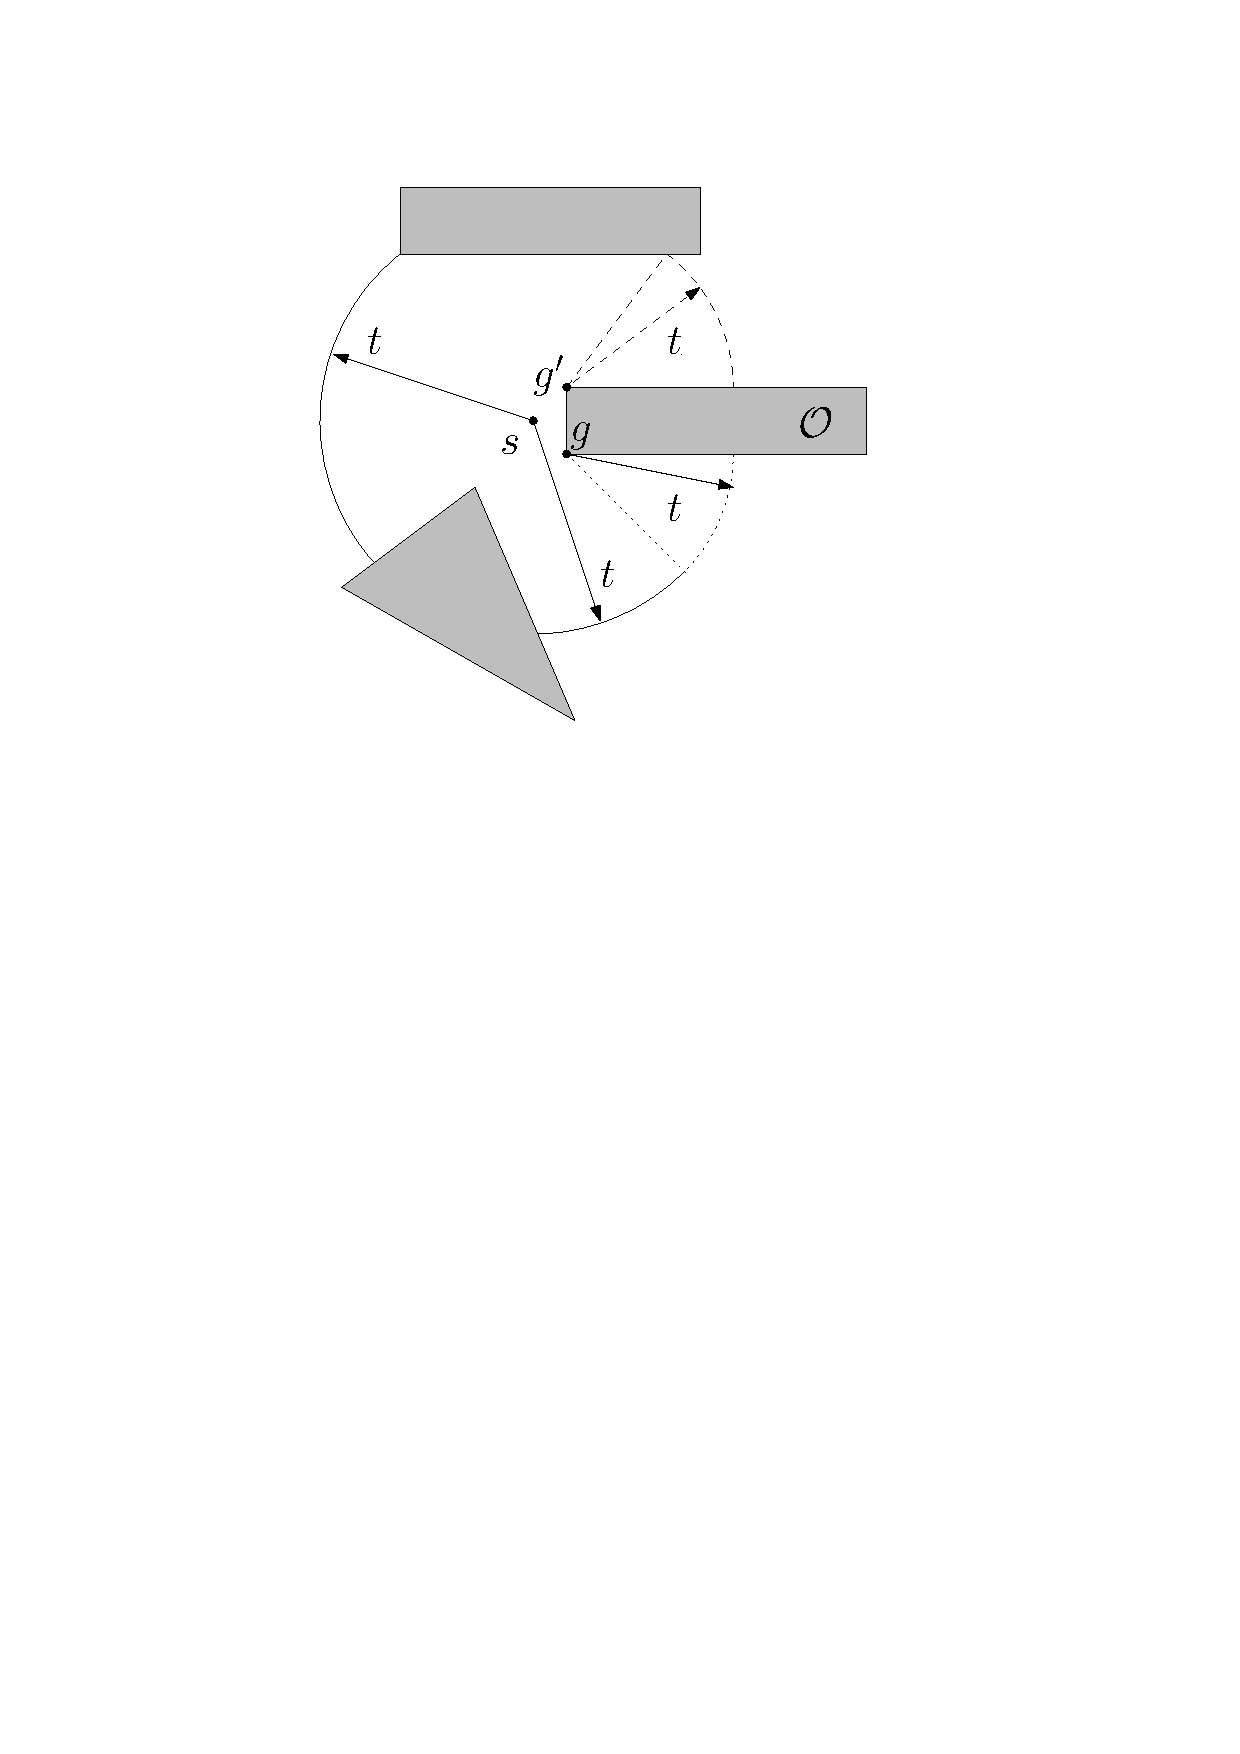
\includegraphics[width=0.45\textwidth]{figures/wavefrontpropagation.pdf}
	\caption{An example of a wavefront propagation from $s$ with distance $t$ to all
    		 points of its circular arch. Since a path into the dashed and dotted 
             area would require a turn at $O$, these areas are propagated 
             by $g$ and $g'$. Since we look at the propagation at time $t$ both 
             generator would have propagated a distance $t$.}
	\label{fig:wavefrontpropagation}
\end{figure}

As the wavefront expands, the meeting point of two adjacent wavelets sweeps along a 
\textit{bisector curve}, and divides the area between them with a hyperbolic bisector 
of the two wavelets generators\footnote{see appendix A}. These ideas can be seen on 
figure \ref{fig:bisectorex}. Here $g$ and $g'$ are generators, who each starts a 
wavelet marked by the dotted line. These two wavelets meets, and for every point they 
meet, the shortest distance from this point has equal length to both $g$ and $g'$. 
This is what creates the horizontal line between $g$ and $g'$, which is the 
hyperbolic bisector. The wavefronts creates paths, which have their endpoints when 
the wavelet meet obstacles, or the planes outer boundary. These endpoints sweeps 
along the obstacle boundaries as the wavefront expands. 

From the above we see that the topology, or "shape", of wavefronts during the 
simulation changes in the case of two different event: wavefront-wavefront collisions 
 and wavefront-obstacles collisions. 

\begin{figure}[H]
	\centering
	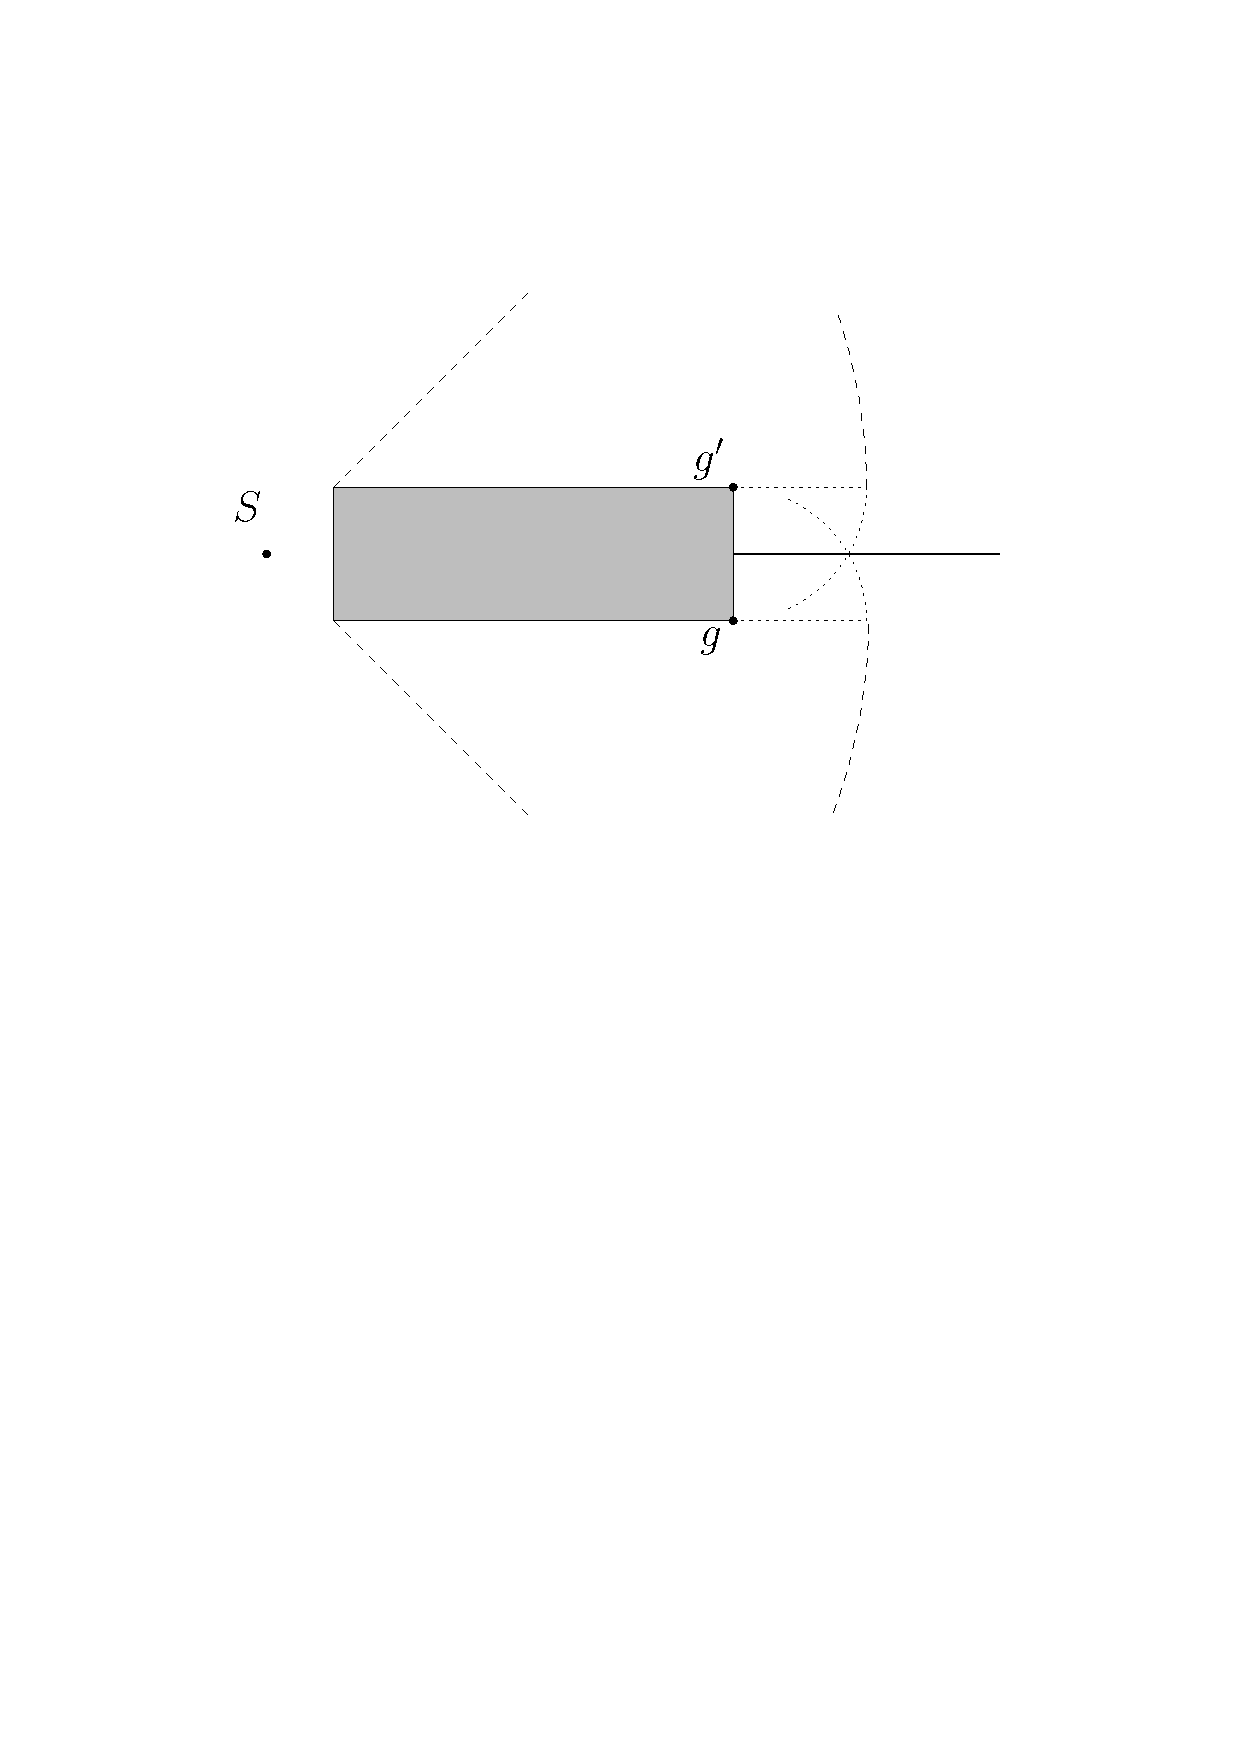
\includegraphics[width=0.45\textwidth]{figures/bisectorex.pdf}
	\caption{The adjacent generator $g$ and $g'$ each produce a wavelets which propagates 
    the space, these are represented by the dotted circular arcs. These will overlap, 
    and the split the area between them into two equal sized regions. The fully drawn 
    line segment between them then represent the splitting point between the two generators, 
    where any point on the line segment, has equal length shortest path to both of the 
    generators.}
	\label{fig:bisectorex}
\end{figure}

\section{Overview of propagation algorithm}

The wavefront propagation algorithm operates in two phases: first a wavefront 
propagation phase, and second a map computation phase. The wavefront propagation 
phase, simulates the wavefront, and thereby determines the approximate locations of 
the different wavefront collision events. We remind that there are two different kind 
of wavefront collisions, the first being the collisions where wavelets are neighbors 
in the wavefronts, that is adjacent wavelets and the collision between them. 
The second being collisions between non-neighboring wavelets. This propagation happens 
through adjacent cells, and only across 
their transparent edges. We remind the reader that transparent edges are the edges 
established by the subdivision, and opaque edges, are the edges of the obstacle 
polygons. The map computation phase uses the information of wavefront collisions to 
build a shortest path map in each cell in the conforming subdivision. 

One of the main idea behind the algorithm, is the idea of calculating two 
"\textit{single-sided approximate wavefronts}" where each approximate wavefronts 
will approach the transparent edge from their own side. This 
idea comes from the fact that literally translating the idea of wavefront propagation  
into an implementation would be very hard. Instead we are contempt with calculating 
for each transparent edge, two \textit{approximate wavefronts}, which will pass 
through the transparent edge, one from each side. So the job of the wavefronts is to 
assign an value $t$ to each point $p$ on an transparent edge. Here $t$ is the time it 
takes to travers at unit speed from the source $s$ to $p$. Each $p$ would have two 
such values, one from each side, where the minimum or these would the one we would use 
for a shortest path. In some cases we determine if a portion of a wavelet $w$ arrives 
after the wavelet $w'$ from the other side has fully engulfed an edge, that there is 
no need to record the time of $w$ since it is so much later than $w'$. This is also a 
reason why we refer to it as approximate, since the approximate wavefront might not 
necessarily give a complete view of all wavelets time to an edge.

\subsection{Definitions and terminology for propagation algorithm}

By visiting the cells in a correct order, and going cell by cell we can calculate the 
correct time in which a wavefront hits a transparent edge, within a giving 
approximation which will be enough for our purpose. To do that we formalize the 
following to sets of edges for an edge $e$, $input(e)$ and $output(e)$.

By $input(e)$ we mean the set of edges whose approximate wavefronts we use when computing 
the approximate wavefront collision with $e$, and as such the distance to $e$. This set 
consists of transparent edges on the boundary of $\mathcal{U}(e)$ which is the well covering 
region of $e$. This is described in section \ref{section:def-well-covering-if-regions}.
Computing the approximate wavefront at $e$ then consist of propagating the approximate 
wavefronts from $input(e)$ to $e$ inside $\mathcal{U}(e)$. It is quite clear that a shortest 
path without violation only needs to bend in the case getting around an obstacle, and the 
same is true for the wavefront. Because $\mathcal{U}(e)$ neither needs to convex, or even 
simply connected, nonconvexity of $\mathcal{U}(e)$ can block the wavefronts from some edges 
of $input(e)$ from reaching $e$. Typically, paths corresponding to blocked wavefronts either 
pass through free space outside $\mathcal{U}(e)$ and re-enter through other edges of 
$input(e)$ of simply run into obstacles outside $\mathcal{U}(e)$. 

By $output(e)$ we refer to the set of edges where $e$ influences the approximate wavefront. 
Formally we define $output(e)$ as 

$$output(e) = input(e) \cup \{ f | e \in input(f) \}$$

The reason $output(e)$ contains $input(e)$ is the algorithm is depending on $output(e)$ 
having a cyclic enclosing of $e$ for detecting wavefront collision events.

\begin{Lemma}[Lemma 4.1 in \cite{HershbergerS99}] \label{lemma:4.1} \hspace{1cm} \\
For any transparent edge $e$, $output(e)$ contains a constant number of edges.
\end{Lemma}
\begin{proof}
	Due to $|\mathcal{U}(f)| = O(1)$ for all edge $f$, and each $\mathcal{U}(f)$ being a 
    connected set of cells of $\mathcal{S}'$, no edge $e$ can belong to $input(f)$ for more 
    than $O(1)$ edges $f$.
\end{proof}

The implementation of the wavefront propagation is loosely synchronized. A main idea of 
approximate wavefront propagation being approximate lies in the following implementation: 
For a transparent edge $e=\overline{ab}$ we define 

$$\tilde{d}(s,e)=\min(d(s,a),d(s,b))$$ 

This estimates $d(s,e)$ because if the wavefront hits $a$ or $b$ then $\tilde{d}(s,e) = 
d(s,e)$, with $d(s,e)$ being the real distance from $s$ to $e$. Should the wavefront hit 
right in the middle, between the endpoints of $\overline{ab} = e$, then the distance to $a$ and 
$b$ from the point the wavefronts collides with would be $\title{d}(s,e)=d(s,e)+\frac{1}
{2}|e|$. Since if we, in the later case, move the point of collision in any direction the 
distance becomes smaller, since it must hold that $d(e,s) \leq \tilde{d}(e,s) \leq d(e,s) + 
\frac{1}{2}|e|$. 

Since we want to compute the covering time of each $e$, i.e. the time at which $e$ is 
completely covered by the wavefront. We set the time to $\tilde{d}(s,e)+|e|$. It is 
obviously a conservative estimate of when the whole edge is fully covered. This time can 
easily be calculated on the fly and only be looking at the $input(e)$. We denote the time 
where the edge $e$ is fully covered by $covertime(e)$. 

\subsection{The propagation algorithm, main loop}

Initially we look at every $e$ that is in the well-covering region $\mathcal{U}(e)$ (which 
also includes the source point $s$). We proceed to calculate an upper bound on $\tilde{d}
(s,e)$ considering only straight-line paths inside $\mathcal{U}(e)$ and set the 
$covertime(e) = \tilde{d}(s,e) + |e|$. For all other edges $e$ we initialize $covertime(e) = 
\infty$. This implies if the $covertime(e)$ is set to $\infty$, then the shortest path 
$\pi(s,a)$ or $\pi(s,b)$ must exit the boundary of $\mathcal{U}(e)$.

The algorithm for simulation, maintains a time parameter $t$ and processes each edge in 
order of its covertime. The main loop of the simulation is as follows:

\begin{algorithm}[H]
	\caption{Propagation Algorithm} \label{algorithm:propagationalgorithm}
	\begin{algorithmic}[1]
		\While {there is an unprocessed transparent edge}
        	\State Select edge $e$ with minimum $covertime(e)$
            \State Set time $t$ to $covertime(e)$
            \State \multiline{compute the approximate wavefronts at $e$ 
            		based on the approximate 
        		    wavefronts from all edges $f\in input(e)$ satisfying 
                    $covertime(f) < covertime(e)$}
            \State Compute $d(s,v)$ exactly for each endpoint $v$ of $e$.
            \ForEach {edge $g \in output(e)$}
           		\State \multiline{Compute time $t_g$ when approximate wavefront 
                	   from $e$ first engulfs an endpoint of $g$}
                \State Set $covertime(g)$ to $\min(covertime(g), t_g + |g|)$.
            \EndFor
        \EndWhile
	\end{algorithmic} 
\end{algorithm}

Lemma \ref{lemma:4.2} provides a proof of the propagation algorithms consistency, by showing 
$covertime()$ is correctly maintained and the edges needed for processing $e$ would already have 
been processed. 

\begin{Lemma}[Lemma 4.2 in \cite{HershbergerS99}]\label{lemma:4.2}
During the wavefront propagation the following invariants hold:

\begin{enumerate}[(a)]
	\item If a wavefront of an edge $f \in input(e)$ contributes to an
	approximate wavefront of e then $\tilde{d}(s,f)+|f|<\tilde{d}(s,e)+|e|$.
	\item The value of $covertime(\cdot)$ is updated a constant number of times.
	\item The final value of $covertime(e)$ is $\tilde{d}(s,e)+|e|$. This value
	is reached no later than the simulation clock reaches that time.
%side 16
	\item Edge e is processed at simulation time $\tilde{d}(s,e) + |e|$
	\end{enumerate}
\end{Lemma}

\begin{proof} 
The parts of the lemma are proven individually

	(a) If a wavelet is able to contribute to the approximate wavefront at $e$
	it must be the case that it reaches $e$ at some time $t_e$ where $d(e,s) \leq
	t_e \leq \tilde{d}(s,e)+|e|$. 
	On the way from $s$ to $e$ the wavelet either goes straight from $s$ in side 
	$\mathcal{U}(e)$ or by going through another transparent edge  $f \in inpute(e)$ at an 
    earlier time $t_f$ 
	with $d(s,f) \leq t_f < \tilde{d}(s,f)+|f|$ and $t_e \geq t_f+d(f,e)$.  
	Since we know from $(W3_{fs})$ of a well-covering region with parameter 2, 	   
    $d(f,e)\geq 2|f|$	
	and so $t_e \geq d(s,f)+2|f|$. Since $\tilde{d}(s,f)+\frac{1}{2}|f|$, it
	must be the case that $\tilde{d}(s,f)+|f|<\tilde{d}(s,e)+|e|$. \\

	(b) The value of $covertime(e)$ is only updated when an edge $f$ is processed
	from either $f \in input(e)$ or $e \in input(f)$. There are $O(1)$ such edges by
	Lemma \ref{lemma:4.1} \\

	(c),(d) These are proven by induction on the simulation clock. (c) and
	(d) holds for the edges $e$ whose initial $covertime(e)$ values are not
	infinite. The wavelets that first reaches an endpoint of $e$, at
	$t_e=\tilde{d}(s,e)$ passes through some $f \in input(e)$. Because of the
	base-case in the induction we know that $f$ has has already been visited before the 
    simulation clock
	reaches $t_e$ and so $covertime_e$ is set to $\tilde{d}(s,e)+|e|$ no later
	than $t_e=\tilde{d}(e,s)$. The variable $covertime_e$ cannot be set to any
	smaller value, because no approximate wavefront can reach the endpoints of
	$e$ earlier than $\tilde{d}(s,e)$. It follows that $e$ will be processed at
	simulation time $\tilde{d}(s,e)+|e|$.
\end{proof}

\begin{Lemma}[Lemma 4.3 in \cite{HershbergerS99}] \label{lemma:4.3}
	For every vertex v of our conforming subdivision, the propagation algorithm
	correctly determines the distance $d(s,v)$ before $v$ is used as a generator in
	any wavefront.	
\end{Lemma}

\begin{proof}
	In a conforming subdivision, every vertex $v$ is an endpoint of a transparent edge 
    $e$. The wavefront that creates the distance $d(s,v)$, either reaches $v$ by only 
    traveling within the boundary of $\mathcal{U}(e)$ or exists through an edge $f \in 
    input(e)$ s.t. $covertime(f) < covertime(e)$. In the case of not leaving $\mathcal{U}(e)$, 
    the initialization trivially computes $d(s,v)$ correctly. The case of leaving 
    $\mathcal{U}(e)$, step 4 and 5 in algorithm \ref{algorithm:propagationalgorithm} 
    implies $d(s,v)$ would be correctly computed. Should $v$ be an obstacle vertex, it may 
    appear as a generator in a wavefront, but it will not be used until $d(s,v)$ is 
    computed at time $\tilde{d}(s,e)+|e|$ (Lemma \ref{lemma:4.2} (d))
\end{proof}

Even though a well-covering union of cells $\mathcal{U}(e)$ has constant complexity, it might not be 
a simple connected component. One could consider the case of a square annulus. Consequently 
there might be multiple topologically distinct paths from a boundary edge $f \in input(e)$ 
to $e$. But we're not interested in comparing paths of different topologies, so to avoid 
comparisons of different topological paths we split the wavefront $W(e)$ into topologically 
equivalent pieces. 

For this purpose, let $W(e)$ denote one of the approximate wavefront passing through $e$. Now 
when we will compute $W(e)$ from the set $\{W(f) \mid f \in input(e)\}$, we will use topologically 
constrained versions of the two incoming wavefronts, which we will denote $W(f,e)$. In this 
context a wavefront $W(f,e)$ will be a portion of $W(f)$ that follows a single topological 
path inside $\mathcal{U}(e)$ from $f$ to $e$.

To further extend this notation, we can consider a $\mathcal{U}(e)$ which contains holes. 
In this cell there will therefore be multiple topologically distinct paths from an edge $f 
\in input(e)$ to $e$. When distinguishing between the multiple topologically different 
wavefronts from a single edge $f$ to $e$, we will use a primed notation $W(f,e)$, $W(f',e)$ 
etc.

Lets assume that two point $p, q \in e$ are hit by a single topologically constrained 
wavefront $W(f,e)$. The segment of $e$ which has $p$ and $q$ as endpoints then all of the 
segments points has among their predecessor the generator vertices in $W(f)$, which 
intersects $f$ and $e$. Also the quadrilateral\footnote{A figure consisting of 4 vertices in a euclidean space} 
bounded by the segments of $f$ and $e$, which 
is a subset of $\mathcal{U}(e)$. Such paths are not always segments. We can imaging an 
obstacle vertex $v$ which lies in a well-covering region of $e$, and the path from $f$ to $p$ 
turns at $v$. This would then imply that the predecessor of $p$ in $W(f,e)$ may be $v$. 
Should this be the case, then the paths from $p$ and $q$ to $f$ can be continuously deformed 
(there is no obstacles between the two paths) to each inside $\mathcal{U}(e)$. 

Unless source $s \in \mathcal{U}(e)$, then for any points $p \in e$ the shortest path $\pi(s,p)$ 
would pass through some $f \in input(e)$, an so constrain the source wavefronts to pass 
through $input(e)$, and by doing so not lose any essential information for the path.

\subsection{The artificial wavefronts}

As mentioned earlier, conceptually when calculating the distance to a transparent edge $e$, we 
can get to situation where one wavefront will consume the edge way before the other edge even 
reaches $e$. In such a situation we would want to discard the wavefront arriving later, 
because we don't need it since its being dominated. The concept for this is the artificial wavefronts. 
This mechanism will also be our only mechanism for pruning the wavefront that arrives second at a 
transparent edge. The easiest way to understand artificial wavefronts is by an example, see figure 
\ref{fig:artificialwavefront} below.

\begin{figure}[H]
	\centering
	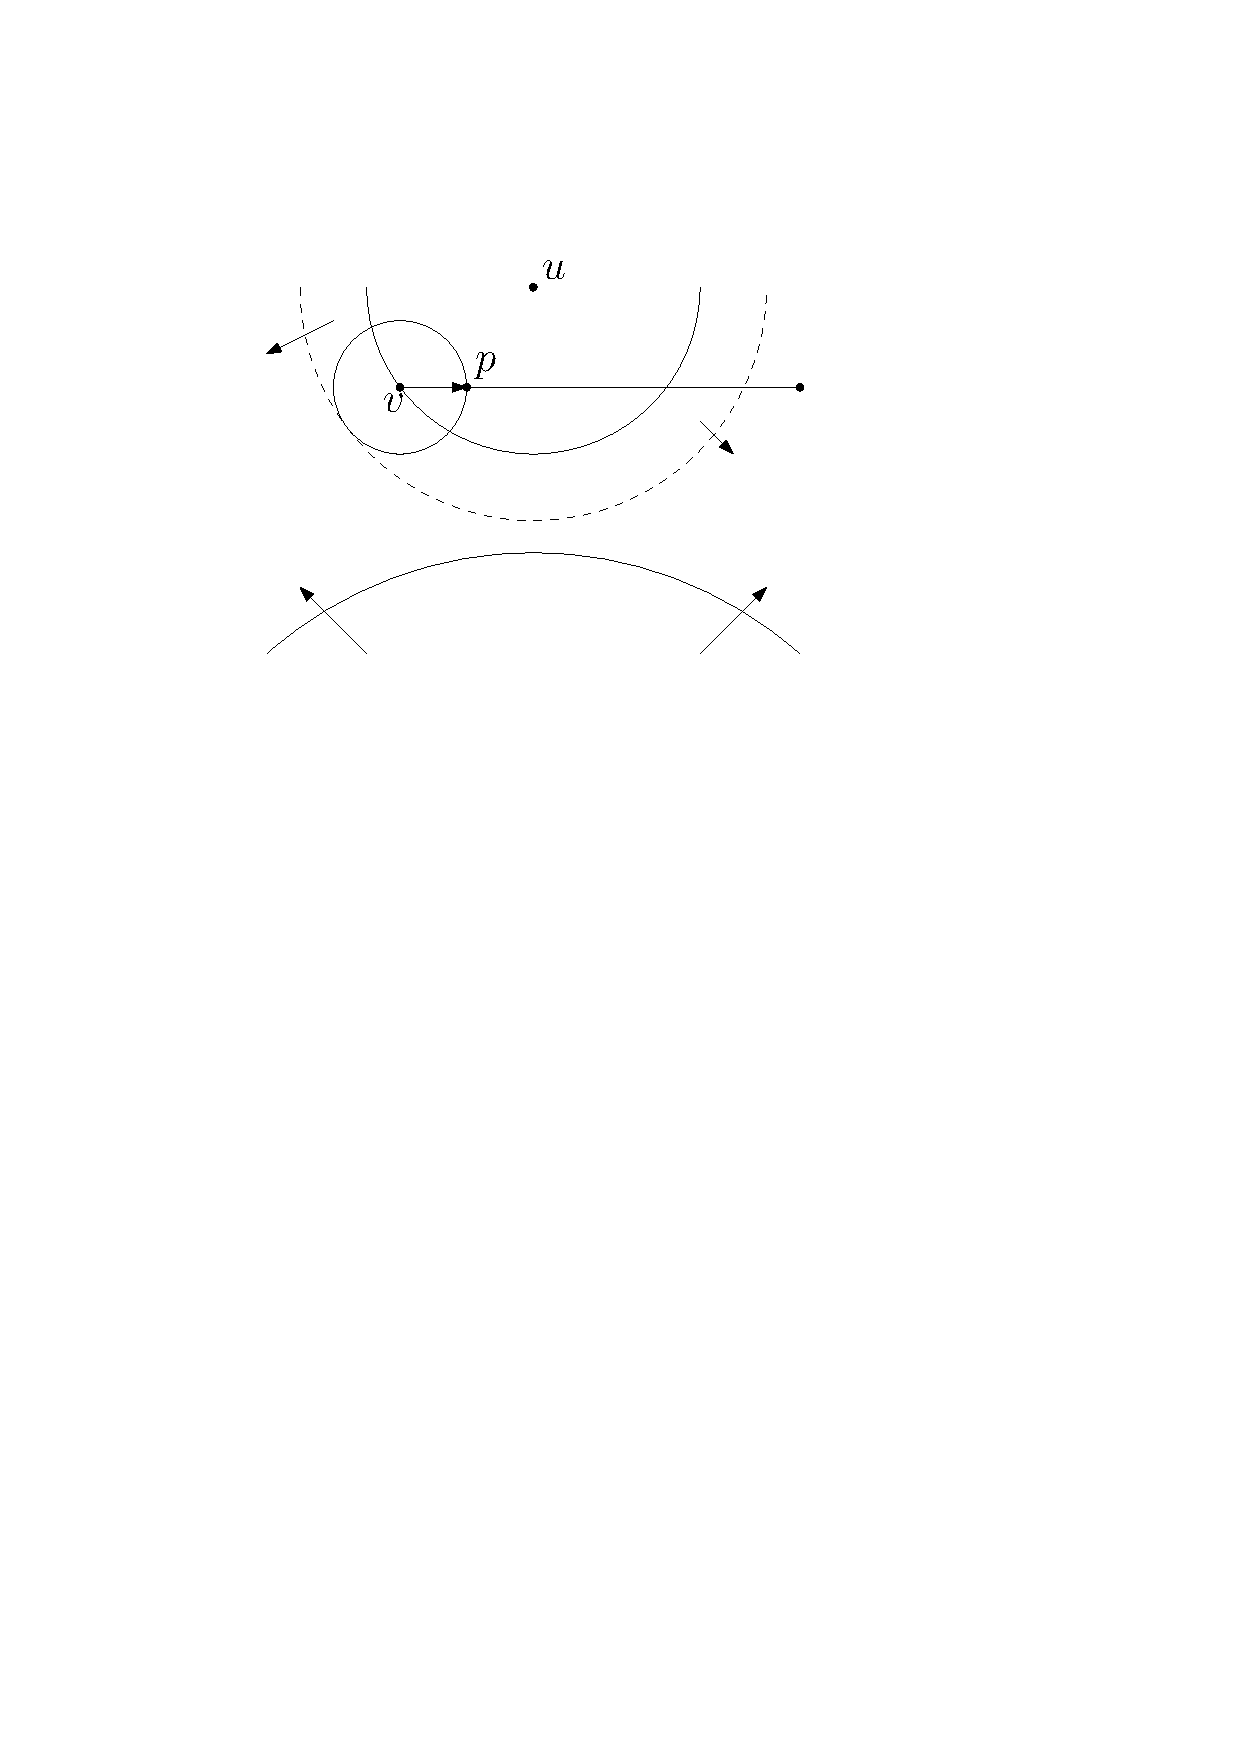
\includegraphics[width=0.45\textwidth]{figures/artificialwavefront.pdf}
	\caption{An example of an artificial wavefront from $v$ reaching point $p$ on edge $e$\cite{HershbergerS99}}
	\label{fig:artificialwavefront}
\end{figure}

Here $u$'s wavefront engulfs the left side of the transparent edge below it, lets call it $e$. 
The left endpoint of $e$ is $v$. When $v$ is engulfed, $v$ will generate a artificial wavefront, 
which will run along $e$. In the figure we see that $v$'s artificial wavefront engulfs $p$ 
before the wavefront from the other side even reaches $e$. By the triangular inequality we 
have $d(s,p) \leq d(s,v) + |\overline{vp}|$ for any point $p \in e$. This surely means that 
the upper wavefront reaches $p$ first, and there is therefore no need to continue the 
propagation of the lower wavefront through $p$.

So when computing the approximate wavefront passing through $e$ from below, the contributing 
wavefronts are the following:

\begin{enumerate}
\item All wavefront $W(f,e)$ for $f \in input(e)$ and $f$ below the line supporting $e$. As 
mentioned before, we differentiate between paths of topological difference, so if $f$ 
intersect the line supporting $e$, we then split $W(f,e)$ into two, and keep only the portion 
$W(f',e)$ that comes from the part of $f$ below $e$.
\item An artificial wavefront expanding from each endpoint of $e$. These generator, e.g. $v$ 
from figure \ref{fig:artificialwavefront} has weight $d(v,s)$.
\end{enumerate}

So in essence, the artificial wavefront is a convenient mechanism for discarding parts of the 
actual wavefront which will be completely dominated by other parts of the wavefront. Since we 
only use of the artificial wavefronts to discard parts of incoming wavefronts, their generators 
will not be passed on to $output(e)$ as part of the approximate wavefront, unless it's also a 
vertex of the set of obstacles $\mathcal{O}$.

\subsubsection{Proof for artificial wavefronts}

The following proofs are taken from \cite{HershbergerS99}, and included for completeness.

Consider a set of wavefronts that reach $e$ from the same side. We say that a
contributing wavefront $W(f)$  claims a point $p \in e$ if $W(f)$ reaches $p$
before any other contributor from the same side of $e$.

\begin{Lemma}[Lemma 4.4 in \cite{HershbergerS99}] 
	Let $e$ be horizontal  and let $W(f,e)$ and $W(g,e)$ be two contributors to the
	approximate wavefront that passes through $e$ from below. Let $p$ and $p'$ be
	points on $e$ claimed by $W(f,e)$ and let $q$ be a point $e$ claimed by $W(g,e)$. The
	$q$ cannot lie between $p$ and $p'$.
\end{Lemma}

\begin{proof}
	Consider the the shortest paths $\pi(s,p)$, $\pi(s,p'),$ and $\pi(s,q)$ in
	the modified environment in which $e$ has been replaced by an open, opaque
	segment. These paths connect $p$ and $p'$ to $f$ and $q$ to $g$, inside
	$\mathcal{U}(e)$. Shortest paths $\pi(s,p)$, $\pi(s,p'),$ and $\pi(s,q)$ do
	not cross. The subpaths of $\pi(s,p)$ and $\pi(s,p')$ inside
	$\mathcal{U}(e)$ can be continuously deformed to each other inside
	$\mathcal{U}(e)$, so $g$ is not between them. It follows that $q$ is not
	between them, either.
\end{proof}

\begin{Lemma}[Lemma 4.5 in \cite{HershbergerS99}]
	Let u and v be two obstacle vertices, both generating wavelets that are
	considered when the approximate wavefront passing through an edge e from
	below is computed. Then the bisector generated by u and v intersects e at
	most once in SPM(s).
\end{Lemma}

\begin{proof}
	Suppose the bisector intersects $e$ twice. Without lose of generality assume
	$u$ lies inside the loop formed by the bisector and $e$. If the bisector
	intersects $e$ twice in $u$ lies inside the loop formed by the bisector and
	$e$. If the bisector intersects $e$ twice in $SPM(s)$, then the segment from
	$u$ to its predecessor must intersect $e$ between the two bisector
	intersections.  The means that $d(e,s)<d(u,s)$, in fact, $d(e,s)+2|e|\leq
	d(u,s)$. Hence $\tilde{d}(e,d)+|e| < d(u,s)$ and $u$ cannot contribute to
	the approximate wavefront at $e$: it does not become a generator until after
	$e$ is prcoessed, contradicting the assumption that both $u$ and $v$
	contribute to the approximate wavefront at $e$.
\end{proof}

\begin{Lemma}[Lemma 4.6 in \cite{HershbergerS99}] \label{lemma:4.6HersherbergerS99}
	Given $W(f,e)$	for each f below e that contributes to $W(e)$ we can compute
	the interval of e claimed by each $W(f,e)$ in $O(1+m)$ total time, where $m$
	is the total number of generators in all wavefronts $W(f,e)$ that are absent
	from $W(e)$.
\end{Lemma}

\begin{proof}
	For each contributing wavefront $W(f,e)$, we show how to determine the
	portion of e claimed by $W(f,e)$ if only one other contributing wavefront
	$W(g,e)$ is present. Lemma 4.4 implies that this portion is contiguous. The
	intersection of these  claimed portions taken over all other contributors
	$W(g,e)$, is part of $e$ claimed by $W(f,e)$ in $W(e)$.

	In constant time we determine whether the claim of $W(f,e)$ is left or right
	of that of $W(g,e)$. If both $W(f,e)$ and $W(g,e)$ reach the left endpoint
	of $e$ in constant time, check which one reaches it sooner. Otherwise one of
	$W(f,e)$ and $W(g,e)$ reaches a point on $e$ that is left of any point
	reached by the other, and this point determines the ordering. Without loss
	of generality, assume that the claim of $W(f,e)$ is left of that of $W(g,e)$

	By Lemma 4.4 we can combine the two wavefronts using only local operations.
	Let $a$ denote the generator in $W(f,e)$ claiming the rightmost point on
	$e$. Let $p_a$ be the left endpoint of $a$'s interval on $e$. Similarly, let
	$b$ denote the generator in $W(g,e)$ claiming the leftmost point on $e$ and
	let $p_b$ be the right endpoint of $b$'s interval on $e$. Compute the
	bisector of $a$ and $b$, and let its intersection with $e$ be the point $x$.
	(By Lemma 4.5 there is only one intersection poiny in $SPM(s)$. If the
	hyperbola generated by $a$ and $b$ intersects $e$ twice, then $a$ is to the
	left of $b$ at only one of the intersections, and we use that intersection
	as $x$.) See figure 4.2. If $x$ is to the left of $p_a$, then delete a from
	$W(f,e)$ if $x$ is to the right of $p_b$, then delete $b$ from $W(g,e)$ in
	either case redefine $a$, $b$, $p_a$, $p_b$ recompute $x$, and repeat this
	test. If $p_a$ is left of $p_b$ and x lies between them then $x$ is the
	right endpoint of $W(f,e)$'s claim in the presence of $W(g,e)$
	
    \begin{figure}[H]
	\centering
	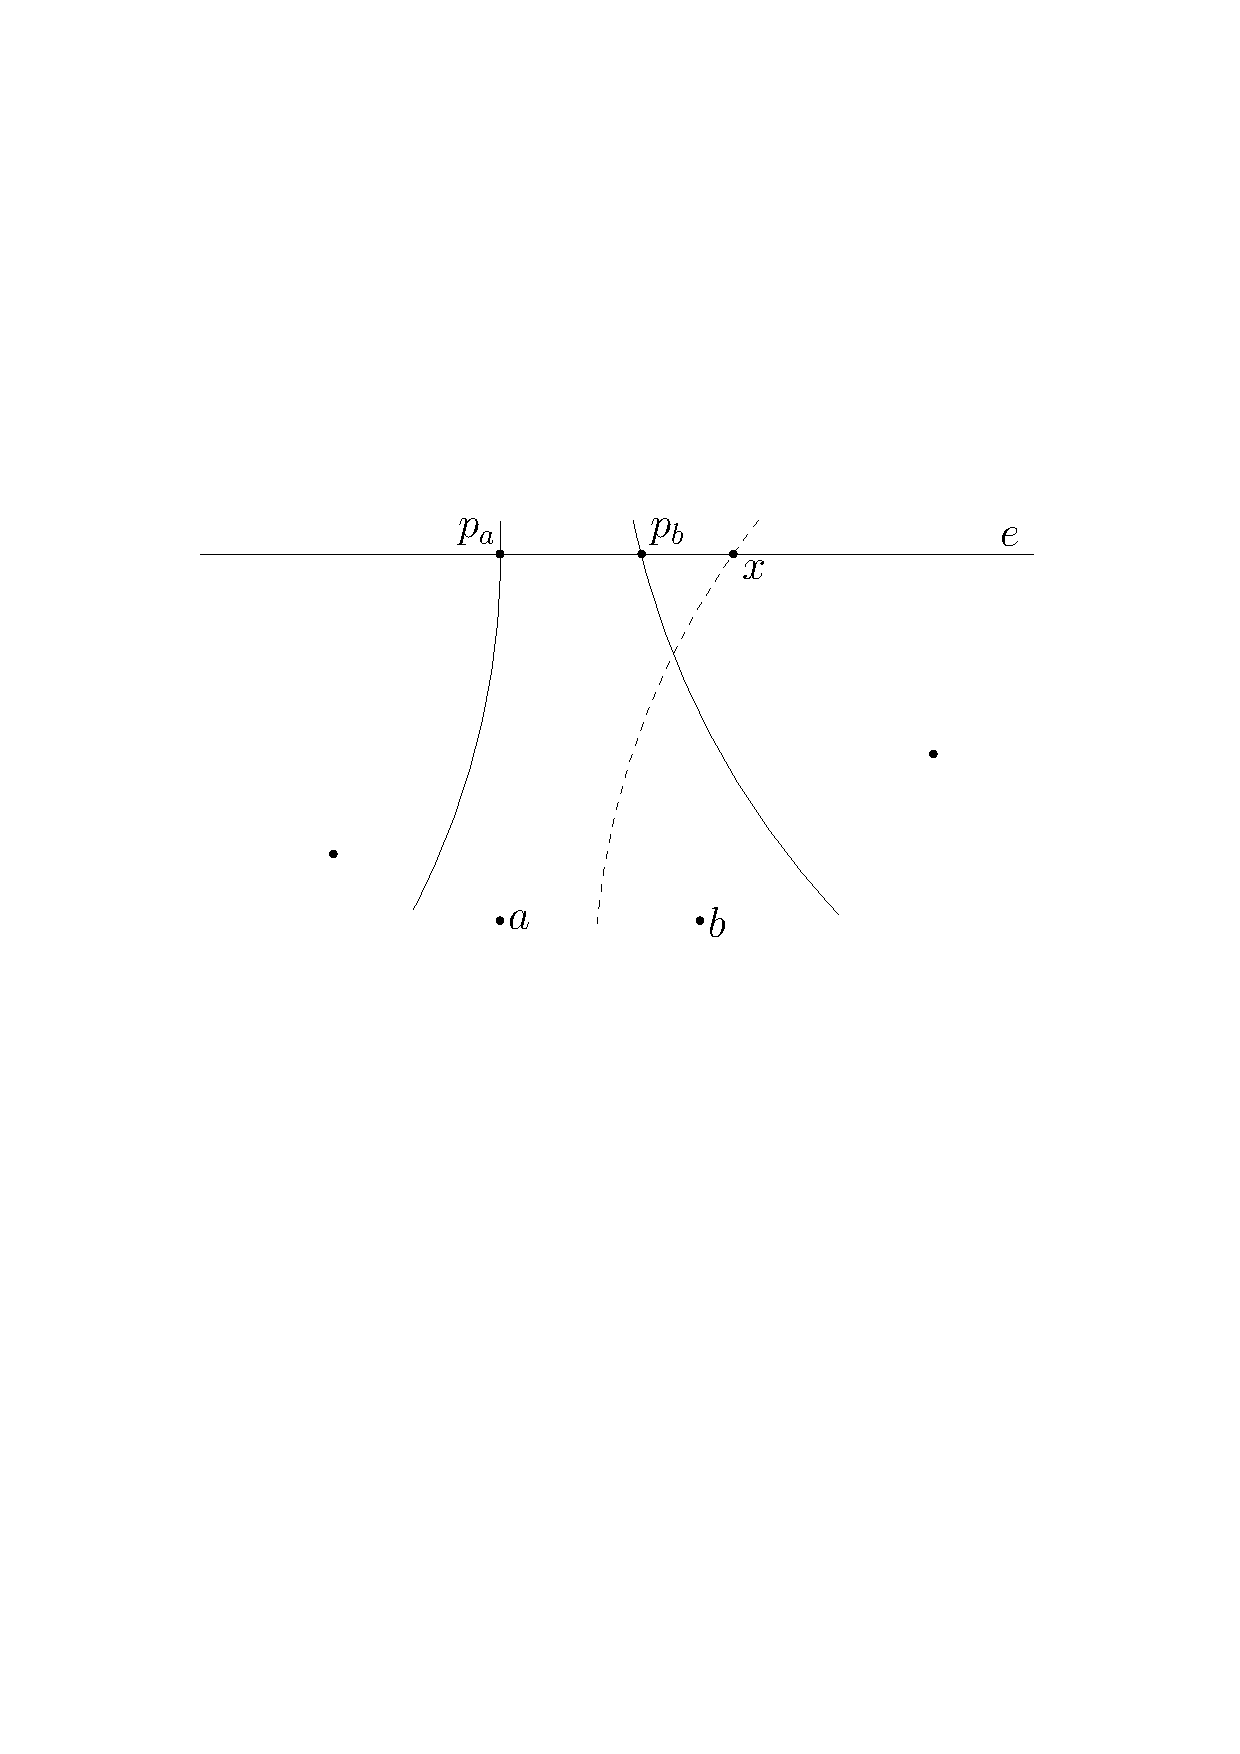
\includegraphics[width=0.65\textwidth]{figures/contribution.pdf}
	\caption{The contribution of $b$ to $W(e)$ is constrained to be left of $p_b$ 
    		 and right of $x$ and therefore does not exist\cite{HershbergerS99}.}
	\label{fig:artificialwavefront}
	\end{figure}

	By combining the claimed regions for all contributors $W(f,e)$ we construct
	the approximate wavefront $e$. The time bound follows since spend constant
	time per generator that is deleted for each pair of wavefronts, and he total
	number of wavefronts $W(f,e)$ to be merged is also constant. This finishes
	the proof
\end{proof}
\begin{Lemma}
	Any generator deleted during the construction of an approximate wavefront at
	edge $e$ does not contribute to the true wavefront at $e$. Every generator
	that contributes to the true wavefront at $e$ either is $s$ or belongs to
	one of the approximate wavefronts at $e$.
\end{Lemma}
\begin{proof}
	The first part is clear since every deleted generator is dominated by some other
	generator at $e$. The second part follows by induction from two facts: any
	wavelet that contributes to the true wavefront at $e$ must come either from
	$s$ inside $\mathcal{U}(e)$ or through one of the edges in $input(e)$ (by
	the definition of well-covering). The approximate wavefronts at $input(e)$
	are ready before they are needed to construct $W(e)$ (by Lemma 4.2)
\end{proof}

\subsection{The bisector events} \label{section:bisectorevents}

First we remind the reader that when we speak of bisectors, we refer to the meeting points of 
two adjacent wavelets along a bisector curve, which divides the area between them with a 
hyperbolic bisector, see figure \ref{fig:bisectorex}. When we talk about bisector events we 
mean the event of intersections of bisectors with each other or with obstacles. These may 
happen when we propagate an approximate wavefront $W(e)$ to $output(e)$. These bisector event 
may be detected in two ways:

\begin{enumerate}
\item During the computation of $W(e,g)$ from $W(e)$ for some $g \in output(e)$. This kind of 
	  bisector event is detected when simulating the propagation of wavefront from $e$ to $g$ 
      to compute $W(e,g)$. In particular, when two generators $u$ and $v$ are non-adjacent in 
      $W(e)$, but at any time in the propagation from $e$ to $g$ become adjacent, then there 
      is a bisector event involving $u$ and $v$.
\item During the merging process described in Lemma \ref{lemma:4.6HersherbergerS99}. Let a 
	  generator $v$ be contributing to one of the input wavefronts $W(e,g)$, but not the the 
      merged wavefront $W(g)$ at $g$, then $v$ will be involved in the bisector event on the 
      way from $e$ to $g$.
\end{enumerate}

The algorithm for detecting bisector events, detects these in a small proximity to their 
actual location in $SPM(s)$. The process of doing this is by \textit{marking} the generators 
that participate in a bisector event in $O(1)$ cell near where the event is detected. So if a 
generator $v$ is involved in a bisector event in a cell $c$, then $v$ is guaranteed to belong 
to a set of marked generators for $c$. It may however be the case that the set of marked 
generators for a cell $c$ is a super set of generators that actually participate in bisector 
events in $c$. The proof of showing that this total number of generator marked in all the cell 
in $O(n)$ time will be shown in Lemma \ref{lemma:4.9HershbergerS99}

We here state the rules for Marking generators as given in \cite{HershbergerS99}.

\begin{enumerate}
\item If a generator $v$ lies in a cell $c$, them mark $v$ in $c$.
\item Let $e$ be a transparent edge, and let $W(e)$ be the approximate wavefront coming from 
	  some generator $v$'s side of $e$.
      \begin{enumerate}[a.]
      \item If $v$ claims an endpoint of $e$ in $W(e)$, or if it would do so except for an 
            artificial wavefront, then mark $v$ in all cells incident to the claimed endpoint.
      \item If $v$'s claim in $W(e)$ is shortened or eliminated by an artificial wavefront, 
      		then mark $v$ in the cell on $v$'s side of $e$.
      \end{enumerate}
\item Let $e$ and $f$ be two transparent edges with $f \in output(e)$. Mark $v$ in both the 
	  cells that have $e$ as an edge if one of the following event occurs:
      \begin{enumerate}[a.]
      \item $v$ claims an endpoint of $f$ in $W(e,f)$;
      \item $v$ participates in a bisector event detected either during the computation of 
      		$W(e,f)$ from $W(e)$, or during the merging step at $f$. We also mark $v$ as 
            having a bisector event if $v$'s claim of $W(f)$ is shortened by an artificial 
            wavefront.
      \end{enumerate}
\item If $v$ claims part of an opaque edge when it is propagated from an edge $e$ toward 
	  $output(e)$, mark $v$ in both cells with $e$ on their boundary.
\end{enumerate}

From the above we see that both rule 2a and 3a apply when a wavefronts claims an endpoints of 
an edge $e$. The difference lies in 2a marking cells near the claimed end point while 3a  
marks generators in cells near the source edge of the wavefront.

%%%%%%%%%%%%%%%%%%%%%%%%%%%%%%%%%%% Copied from article %%%%%%%%%%%%%%%%%%%%%%%%%%%%%%%%%

\subsubsection{Proof for bisector events}

The following proofs are taken from \cite{HershbergerS99}, and are included for completeness.

A generator may contribute to a wavefront more than once in the wavefront sequence; each mark 
applies to only one instance of the generator in the sequence. The following technical lemma 
is used in the proof of Lemma \ref{lemma:4.9HershbergerS99} to establish the correctness of 
the marking rules.

\begin{Lemma}[Lemma 4.8 in \cite{HershbergerS99}] \label{lemma:4.8HershbergerS99}
	Let $v$ be a generator that contributes to an approximate wavefront $W(e)$
	suppose there is a point $p \in e$ that is claimed by $v$ in $W(e)$ but not
	in $SPM(S)$ (because a wave from the other side of $e$ reaches $p$ first)
	Then $v$ is marked in the cell $c$ on $v$'s side of $e$.
\end{Lemma}
\begin{proof}
	If $v$ is unmarked in $c$ there must be generators $u$ and $w$ such that
	$u$, $v$, $w$ are consecutive in $W(e)$ --- otherwise  Rule 2 would
	apply. The bisectors $(u,v)$ and $(v,w)$ must exit from $\mathcal{U}(e)$
	though the same transparent edge $h$ --- otherwise Rule 3 or 4 would
	apply. For the same reason, the region bounded by $(u,v)$, $(v,w)$, $h$,
	and $e$ is a subset of $\mathcal{U}(e)$ --- if the region contained a
	non-$\mathcal{U}(e)$ island, $v$ would claim an endpoint of a boundary
	edge of that island. Edge $h$ is by definition part of $input(e)$.
	Consider the point $p \in e$ that is claimed by $v$ in the approximate
	wavefront $W(e)$ but not in the true wavefront at $e$, and suppose that
	the true predecessor of $p$ is $z\neq v$. The vertex $z$ is either an
	obstacle vertex or the source $s$. In the former case, $z$ lies outside
	$\mathcal{U}(e)$ or on its boundary $\partial\mathcal{U}(e)$ --- by
	condition (C3), $\mathcal{U}(e)$ contains at most one obstacle vertex, so
	any vertex not strictly outside $\mathcal{U}(e)$ must be connected to
	points outside $\mathcal{U}(e)$ by opaque edge. Vertex $z$ may lie
	strictly inside $\mathcal{U}(e)$ only if $z=s$.

	Let us first assume that $z$ lies outside the well-covering region
	$\mathcal{U}(e)$ --- the proof simplifies in the other case, which is
	considered below. Let $q$ denote the intersection point between
	$\overline{zp}$ and $input(e)$ closet to $p$ (recall that $input(e)
	\subset output(e)$ and $input(e) \subset \partial\mathcal{U}(e))$. Based
	on the position of $q$ relative  to the bisector $(u,v)$ and $(v,w)$ we
	argue that $v$ must have been involved in a bisector event detected by
	our algorithm and thus marked in cell $c$.

	First consider the case in which $q$ lies between the bisectors $(u,v)$
	and $(v,w)$ on the edge $h$. Now, since $|\overline{qp}|\geq|h|$ (by the
	well-covering property), the endpoints of $h$ are engulfed by a wavefront
	from $z$ or from some other generator before the wavefront from $z$
	reaches $p$ at time $d(s,z) + |\overline{zp}|$. The artificial wavefront
	from $h$'s endpoints will cover $h$ before time
	$d(s,z)+|\overline{zp}|+|h|$. By assumption we have
	$d(s,v)+|\overline{vp}| > d(s,z)+|\overline{zp}|$. The wavefront from $v$
	cannot reach $e$ earlier than $d(s,v)+|\overline{vp}| - |e|$. By
	well-covering with parameter 2, $d(e,h)$ is at least $|e|+|h|$ and so the
	wavefront from $v$ reaches $h$ no earlier than
	$d(s,v)+|\overline{vp}|+|h|>d(s,z)+|\overline{zp}|+|h|$, at which time
	$h$ is already covered by the artificial wavefront. The claim of $v$ on
	$h$ is shortened by the artificial wavefront (in fact $a$'s claim is
	eliminated completely), and so it must be marked by Rule 3b.

	In the second case, $q$ is not between the bisectors $(u,v)$ and $(v,w)$
	on $h$. The segment $\overline{qp}$ must intersect one of the bisectors.
	Without loss of generality, assume $\overline{qp}$ intersects bisector
	$(u,v)$. Since every point on $\overline{qp}$ has $z$ as its predecessor
	in $SPM(s)$, the bisector $(u,v)$ does not reach $\partial\mathcal{U}(e)$
	in $SPM(s)$. We show that our propagation and merging algorithms will
	detect a bisector event for $(u,v)$. Let $r$ be the intersection point
	between the bisector $(u,v)$ and the edge $h$. As noted in the discussion
	after Lemma \ref{lemma:4.3}, the triangle defined by the segments $\overline{ur}$,
	$\overline{vr}$ and $e$ is a subset of $\mathcal{U}(e)$. Bisector $(u,v)$
	crosses the triangle boundary on $e$ and at $r$, but nowhere else. The
	larger region $R$ bounded by $e$, $h$, $\overline{ur}$ and bisector
	$(v,w)$ also is a subset of $\mathcal{U}(e)$ and it contains point $p$.
	Because $\overline{qp}$ crosses into $R$ to intersect $(u,v)$ and it does
	not intersect the $(v,w)$ or $h$ sides of $R$, $\overline{qp}$ must
	intersect $\overline{ur}$ let $x$ be the point of intersection. The
	wavelet from $z$ reaches $x$ before the one from $u$, so the path $z
	\to x \to r$ starting at time $d(s,z)$ reaches $r$ before the path $u \to
	r$ starting at time $d(u,s)$. Observe also that the path $z \to x \to r$
	is a legal path --- it lies in free space. Now, consider the shortest
	path from $z$ to $r$ inside the triangle $\bigtriangleup zxr$ that does
	not cross $h$ or any obstacle edge (see Figure \peter{make figure}). Because $z\to x \to
	r$ lies in free space, such a path exists and is shorter than $z \to x
	\to r$. This path claims $r$ from the same side as $u$ before the wavelet
	from $u$ reaches $r$. (If the path passes through an endpoint of $h$,
	then an artificial wavefront 
	%side 22
	claims $r$ otherwise the last obstacle
	vertex on the path claims $r$.) Thus a bisector event for $(u,v)$ is
	detected during the computation of $W(e,h)$ or $W(h)$ and $v$ is marked
	by Rule 3b.

	Next consider what happens if the predecessor vertex $z$ lies on the
	boundary of the well-covering $\mathcal{U}(e)$. Let $h$ be a boundary
	edge $\mathcal{U}(e)$ incident to $z$. In this case we detect a bisector
	event involving $v$ when we advance the wavefront from $e$ to
	$output(e)$: if $z$ lies between the bisectors $(u,v)$ and $(v,w)$ then
	$v$ is marked by Rule 3a or 4 if $z$ is not between the bisectors, the
	segment $zp$ intersects one of the bisectors, say $(u,v)$ and we detect a
	bisector event for $(u,v)$ in advancing the wavefront from $e$ to
	$output(e)$.

	Finally consider the case in which $z=s$ lies inside $\mathcal{U}(e)$. If
	$z$ is not between the bisectors $(u,v)$ and $(v,w)$ segment
	$\overline{zp}$ intersects one of them and the proof is as above. Let $r$
	be the intersection of $(u,v)$ with $h$ and let $t$ be the intersection
	of $(v,w)$ with $h$. The convex quadrilateral bounded by subsegments of
	$e$, $\overline{ur}$, $h$, and $\overline{tw}$ is contained inside
	$\mathcal{U}(e)$. Hence if $z$ is between the bisectors $(u,v)$ and
	$(v,w)$, the entire segment $\overline{rt}$ is visible from $z$ (that is
	$\bigtriangleup zrt$ is empty) and so $v$'s claim on $h$ is eliminated by
	$z$. Therefore $v$ is marked by Rule 3b. This completes the proof.

\end{proof}
\begin{Lemma}[Lemmma 4.9 in \cite{HershbergerS99}]\label{lemma:4.9HershbergerS99}
	If a generator $v$ participates in a bisector event of $SPM(s)$ in a cell
	$c$, then $v$ is marked in $c$.
\end{Lemma}
\begin{proof}
	If a bisector has an endpoint on an opaque edge of $c$, it either
	emanates from an obstacle vertex on the edge, or it is defined by two
	generators that claim part of the opaque edge. Rule 1 and 4 guarantee
	that all such generators are marked in $c$.
	If a generator $v$ that contributes to an approximate wavefront in $c$ is
	unmarked then by Rule 2a there must be transparent edges $e$ and $f$ on
	the boundary of $c$ such that $W(e)$ and $W(f)$ both contain the
	generator subsequence $u$, $v$, $w$ for some $u$ and $w$.
	Without loss of generality assume $W(e)$ enters $c$ and $W(f)$ leaves
	$c$. If $v$ participates in a bisector event of $SPM(s)$ in $c$, then at
	least one point $p$ inside the region $R$ bounded by $e$, $f$, $(u,v)$
	and $(v,w)$ is not claimed by $v$ in $SPM(s)$. Let $z$ be the true
	predecessor of $p$. Let $r$ and $t$ be the intersections of $(u,v)$ and
	$(v,w)$ with $f$, respectively. Region $R$ is contained in the convex
	quadrilateral $Q$ bounded by $\overline{ur}$, $\overline{rt}$,
	$\overline{tw}$, and the line supporting $e$. Because $u$, $v$, $w$ is a
	subsequence of $W(e)$, no vertex on the same side of $e$ as $v$ claims
	any point of the side of $Q$ collinear with $e$, that is, $\overline{zp}$
	does not cross that side of $Q$. If $r$ and $t$ are both claimed by $v$
	in $SPM(s)$ then $\overline{ur}\in \pi(s,r)$ and $\overline{wt}\in
	\pi(s,t)$. In this case $\pi(s,p)$ cannot cross $\overline{ur}$ or
	$\overline{wt}$ and hence it
	%side 23
	must cross $\overline{rt}$. The intersection of $\overline{zp}$ with
	$\overline{rt}$ is a point $q$ that satisfies the hypothesis of Lemma 4.8,
	and so $v$ is marked in $c$. On the other hand if either $r$ or $t$ is not
	claimed by $v$ in $SPM(s)$ that vertex satisfies the hypothesis of Lemma 4.8
	and so $v$ is marked in $c$.
\end{proof}

The following technical lemma shows that the approximate wavefront are not too
different from the true wavefronts this lets us bound the number of marks made
by the marking rules.
\begin{Lemma}[Lemma 4.10 in \cite{HershbergerS99}] \label{lemma:4.10HershbergerS99}
	Let $B$ be the set of pairs (e,b) of transparent edges e and bisectors b
	such that b crosses e in some approximate wavefront but the same crossing
	does not occur in SPM(s). Then $|B|=O(n)$
\end{Lemma}
\begin{proof}
	Let $(e,b)$ be a pair in $B$. Bisector $b$ is defined by two generators $u$
	and $v$. The proof of Lemma 4.8 notes that each generator (except possibly
	$s$) is outside or on the boundary of $\mathcal{U}(e)$. That proof also
	shows that $b$'s intersection with $e$ in some approximate wavefront (that
	is, the presence of $u$ and $v$ in $W(e)$) is proof that $u$ and $v$ claim
	points on the boundary of $\mathcal{U}(e)$ (in $input(e)$) in $SPM(s)$. Let
	$p=b \cap e$. Because $(e,b)$ is not an incident pair in $SPM(s)$, there
	must be at least one bisector event in $SPM(s)$ that lies in the interior of
	$\mathcal{U}(e)$ between the line segment $\overline{up}$ and
	$\overline{vp}$. We can charge the early demise of $b$ to any one of these
	bisector events.

	The segments $\overline{pu}$ and $\overline{pv}$ are disjoint inside
	$\mathcal{U}(e)$ from the corresponding segments defined by any other pair
	$(e,b') \in B$ in the modified shortest path problem in which the obstacles
	are $O\cup \{e\}$ the segments $\overline{pv}$ and $\overline{pu}$ belong to
	$\pi(s,p)$ and hence they are disjoint from any other such segments. Thus
	the sector bounded by $\overline{pu}$ and $\overline{pv}$ is disjoint inside
	$\mathcal{U}(e)$ from the sector defined by any other pair $(e,b') \in B$ so
	each bisector event inside $\mathcal{u}(e)$ is charged at most once for all
	pairs in $B$ that have $e$ as the first element of the pair. Each cell in
	the conforming subdivision belongs to $O(1)$ well-covering regions
	$\mathcal{U}(e)$. Hence the sum over all transparent edges $e$ of the number
	of bisector events in $\mathcal{U}(e)$ is only $O(n)$. This total is an
	upper bound on $|B|$.
\end{proof}

\begin{Lemma}[Lemma 4.11  in \cite{HershbergerS99}] \label{lemma:4.11HershbergerS99}
	The total number of marked generators over all cells is $O(n)$
\end{Lemma}
\begin{proof}
	We begin by defining a propagation region for each edge $e$. For any
	transparent edge $e$ let $P(e)$ be the collection of cells through which
	wavefronts propagate on the way from $e$ to all edges $f \in output(e)$.
	Clearly $P(e)\subseteq \mathcal{U}(e) \cap \{\mathcal{U}(f)|f\in
	output(e)\}$. The number of cells in $P(e)$ is constant since $|output(e)|$
	is constant and so is the number of cells in $\mathcal{U}(f)$ for any $f$.
	Furthermore since every cell of $P(e)$ is within a constant number of cells
	of $e$, each cell $c$ belongs to $P(e')$ for only a constant number of edges
	$e'$.

	The total number of generator-cell marks made under Rule 1 is clearly $O(n)$

	Each $P(e)$ has constant complexity so there are $O(n)$ edge pairs $(e,f)$
	where $e$ is transparent and $f$ is either transparent and in $output(e)$ or
	opaque and inside or on the boundary of $P(e)$. From this it follows that
	the number of marks made by Rules 2a and 3a is $O(n)$. similarly there are
	$O(n)$ Rule 4 marks in which the wavelet from $v$ claims an endpoint of the
	opaque edge or is the first or last nonartificial wavelet in $W(e)$.

	Any Rule 4 mark not yet counted involves a generator $v$ that does not reach
	any opaque edge endpoint when propagated forward from $e$. Because $v$ is
	not the first or last nonartificial wavelet in $W(e)$, there is a generator
	$u$ such that $v$'s claim on $e$ in $W(e)$ is bounded on the left of
	bisector $(u,v)$. We can assume that $(u,v)$ intersects $e$ in $SPM(s)$ by
	Lemma 4.10 there are only $O(n)$ bisector-edge pairs that intersect in
	approximate wavefronts but not in $SPM(s)$. Bisector $(u,v)$ terminates in
	$P(e)$ either on the opaque edge or in a bisector event before the opaque
	edge. Let us charge the
	%Side 24
	marking of $v$ at $e$ to this endpoint of $(u,v)$ in $SPM(s)$. Because each
	cell belongs to $P(e')$ for a constant number of edges $e'$, each vertex of
	$SPM(s)$ is charged $O(1)$ times. Since $|SPM(s)|=O(n)$, the number of RULE
	4 marks is $O(n)$.

	The proof for rule 2b and 3b are similar to that Rule 4. We begin with the
	proof for Rule 3b. We can assume that the interval claimed by $v$ on $e$ in
	$W(e)$ is bounded by two bisectors $(v,u)$ and $(v,w)$ for two nonartificial
	generator $u$ and $w$ the first and last generators in $W(e)$ counted
	separately sum to at most $O(n)$ overall. Furthermore we can assume that
	$(u,v)$ and $(v,w)$ both intersect $e$ in $SPM(s)$ there are only $O(n)$
	bisector-edge pairs that appear in some approximate wavefront but not in
	$SPM(s)$ (Lemma 4.10). At least one of the two bisector fails to reach the
	boundary of $P(e)$ in $SPM(s)$ because Rule 3b applies and a detected
	bisector event implies the existence of an actual bisector event no later
	than the point of detection we charge the marking of $v$ to that bisector
	endpoint. Each bisector event gets charged $O(1)$ times and there are $O(n)$
	bisector events in $SPM(s)$.

	To bound the number of rule 2b marks, consider where the generator $v$ lies.
	There is at most one generator $v$ inside $\mathcal{U}(e)$ and so $O(n)$
	marks for such generators overall. If $v$ lies outside $\mathcal{U}(e)$
	there is at least one edge in $input(e)$ where $v$ is marked by Rule 3b
	because of the shortening of $v$'s claim on $e$. Charge the Rule 2b mark at
	$e$ to this Rule 3b mark. There are $O(n)$ Rule 3b marks and hence $O(n)$
	Rule 2b marks
\end{proof}
We defer the finer details of the propagation algorithm to section 
\ref{section:implwavefront} and instead describe the second phase of the 
algorithm next, namely the shortest path map computation.

\subsection{Computing the shortest path map}

So far in this section we have gone through the propagation phase. In this phase we have 
propagated the plane with wavefronts and wavelets from generator, and we have used approximate 
wavefronts for each transparent edge to sort out dominated wavefronts. We also marked generators
in every cell $c$, where each marked generator is in the approximate wavefront of one of the 
boundary edges of $c$, an all but $O(1)$ of them contribute to a bisector event either in $c$ or 
in one of $O(1)$ nearby cells. Here the bisector event was the intersections of bisectors with 
each other or with obstacles. The sketch of an algorithm from the proof of Lemma 
\ref{lemma:4.6HersherbergerS99}, will be presented in section \ref{section:implwavefront}, which 
will let us compute the marked generators in $O(\log n)$ time a piece. 

This section is dedicated to show how we can break the interior area of a cell $c$ into 
\textit{active} and \textit{inactive} regions. This splitting will be done on the basis of 
whether a vertex of $SPM(s)$ lie in a region. If it does we denote the area as active, and if 
no vertex is present in the area we denote it as inactive. We saw in section 
\ref{section:bisectorevents}, lemma \ref{lemma:4.9HershbergerS99} that only marked generator 
would contribute to a bisector event in $c$. 

The bisectors made by a marked generators and tehri unmarked neighbors generators will be drawn in the 
$SPM(s)$. All such bisectors are disjoint, and we will see the partition of $c$ into active 
and inactive regions, will be done such that active regions are claimed only by unmarked 
generators and inactive regions by marked generators. This can be seen in figure 
\ref{fig:activeinactiveregions}. 

\begin{figure}[H]
	\centering
	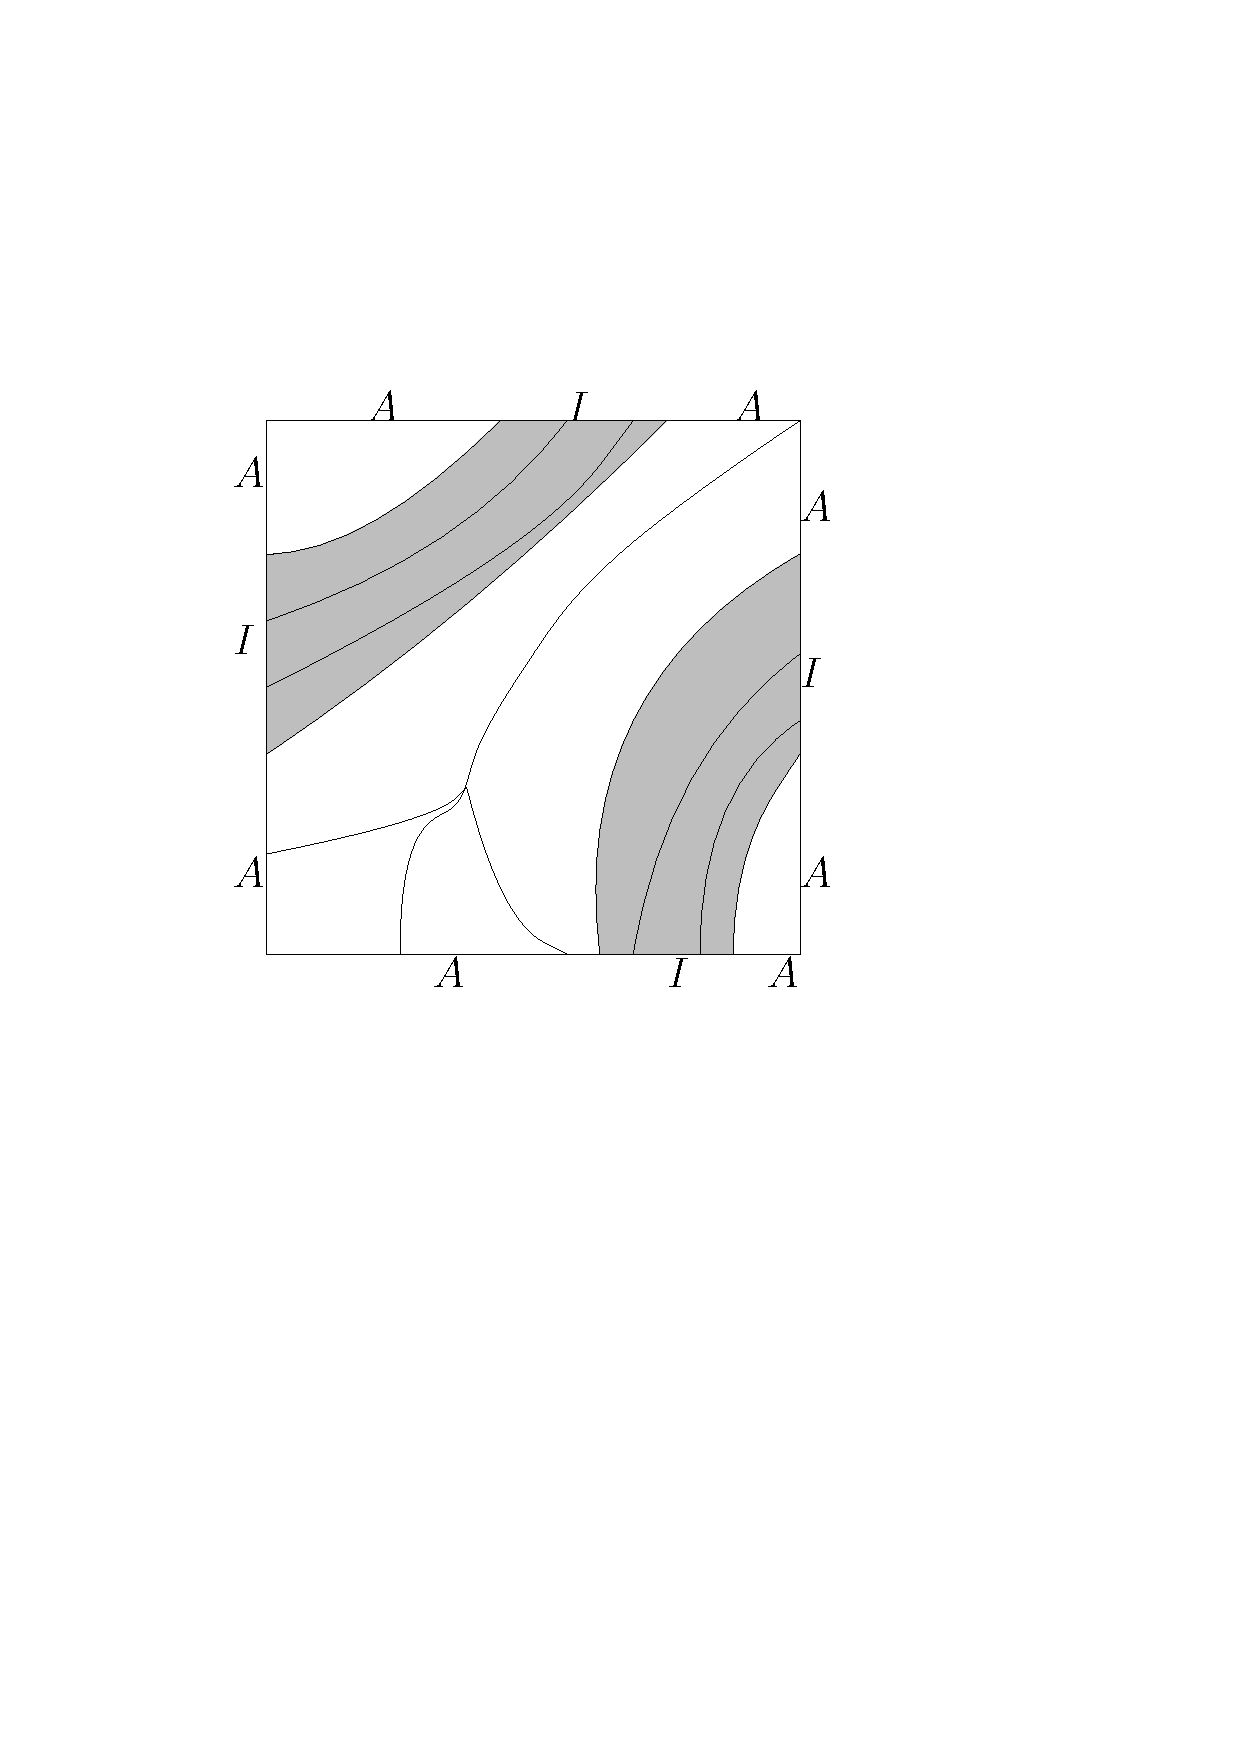
\includegraphics[width=0.5\textwidth]{figures/activeinactiveregions.pdf}
	\caption{Here the white regions are the active regions and the shaded regions are the inactive. The 
    		 boundaries between the regions encapsulating active and inactive region, are 
             defined by being the bisector of one marked and one unmarked generator\cite{HershbergerS99}.}
	\label{fig:activeinactiveregions}
\end{figure}

The algorithm will compute the active regions, which can be done in a time that is proportional to the 
number of marked generators in the cell $c$. Overall can this be done since we know the order of the 
generator along the boundary of $c$, which will help us finding the marked generators with unmarked 
neighboring generators. The calculated boundary of these active regions will have $O(1)$ segments. 
These segments will either be a transparent edge fragment, an opaque edge, of a bisector in $SPM(s)$.

We now let $e$ be a transparent edge fragment that's bounding an active region. Further let $W(e)$ be 
the wavefront that enter the active region by crossing edge $e$. Should $W(e)$ be the only wavefront 
entering through $e$, it will partition the active region into piece which we call $S$-faces. Each 
$S$-face has a unique predecessor in the $W(e)$ partitioning the area. The $S$ faces of an active 
region may not cover all of it, since each point in an $S$-face must be connected to its predecessor 
by a segment that intersect $e$. We define $S(e)$ to be this partition. So basically $S(e)$ are the 
building blocks of a shortest path map, which restricts the active regions and considers only 
generators in $W(e)$. Let assume a point $p$ lies in an $S$-face of $S(e)$ with predecessor $v$, then 
$S(e)$ assigns weight $d(s,v) + |\overline{vp}|$ to $p$. Points outside any $S$-face are assigned 
infinite weight by $S(e)$.

We can compute $S(e)$ in $O(m\log m)$ time, where $m = |W(e)|$, by using the propagation algorithm and 
the auxiliary data structures which will be introduced in section \ref{section:implwavefront}.

\subsubsection{Proof of correctness for computation of SPM}

The following proofs are taken from \cite{HershbergerS99}, and included for completeness.

The following lemma shows how to combine the wavefronts incident to different
boundary edges of an active region.

\begin{Lemma}[Lemma 4.12 in \cite{HershbergerS99}] \label{lemma:4.12} 
	Given the approximate wavefronts on the boundary of a cell $c$ and a set of
	$g$ marked generators in those wavefronts, we can compute the vertices of
	$SPM(s)$ inside $c$ in time $O(g\log g)$.
\end{Lemma}
\begin{proof}
	Consider an active region inside $c$ and two transparent edge fragments $e$
	and $f$ on the boundary of this active region. We can use the merge step
	from a standard divide-and-conquer Voronoi diagram algorithm\cite{CompGeo} to compute the
	portion of the region nearer to $W(e)$ than to $W(f)$ using weighted
	distance in time $O(|W(e)|+|W(f)|)$. More specifically assume that $S(e)$
	and $S(f)$ have both been computed. Let $m=|W(e)|+|W(f)|$. Each of $S(e)$
	defines a distance function on the points of the active region. The
	pointwise minimum of these two functions determines which points are nearer
	to $W(e)$ than to $W(f)$ under weighted distance. Consider a point $p$ in
	the $S$-face for some generator $v\in W(e)$. Point $p$ belongs to $v$'s
	$S$-face in $SPM(s)$ only if all of the segment $\overline{pv}$ is closer to
	$v$ than to any generator in $|W(f)|$. The set of  points $p$ such that the
	entire segment from $p$ to its predecessor is closer to $W(e)$ than to
	$W(f)$ is bounded by a single chain $\Gamma$ of $O(m)$ hyperbolic arcs (see appendix \ref{appendix:def}. (The
	number of arcs follows from Lemma \ref{lemma:3.2}.) To find $\Gamma$, first trace along
	a ray emanating from some generator $v \in W(e)$ marching through $S(e)$ and
	$S(f)$ simultaneously until the ray reaches the boundary of $c$ or reaches a
	point whose weight in $S(f)$ equals its weight in $S(e)$. This takes $O(m)$
	times since a line cuts $O(m)$ edges of $S(e)$ and $S(f)$ containing the
	current point trace along the hyperbola until it leaves one of the two
	$S$-faces then follow the hyperbola determined by the next pair of $S$-faces
	etc. This procedure takes $O(1)$ time per arc of $\Gamma$ or $O(m)$ time
	altogether (see Figure \ref{fig:traceray}). 
    
\begin{figure}[H]
	\centering
	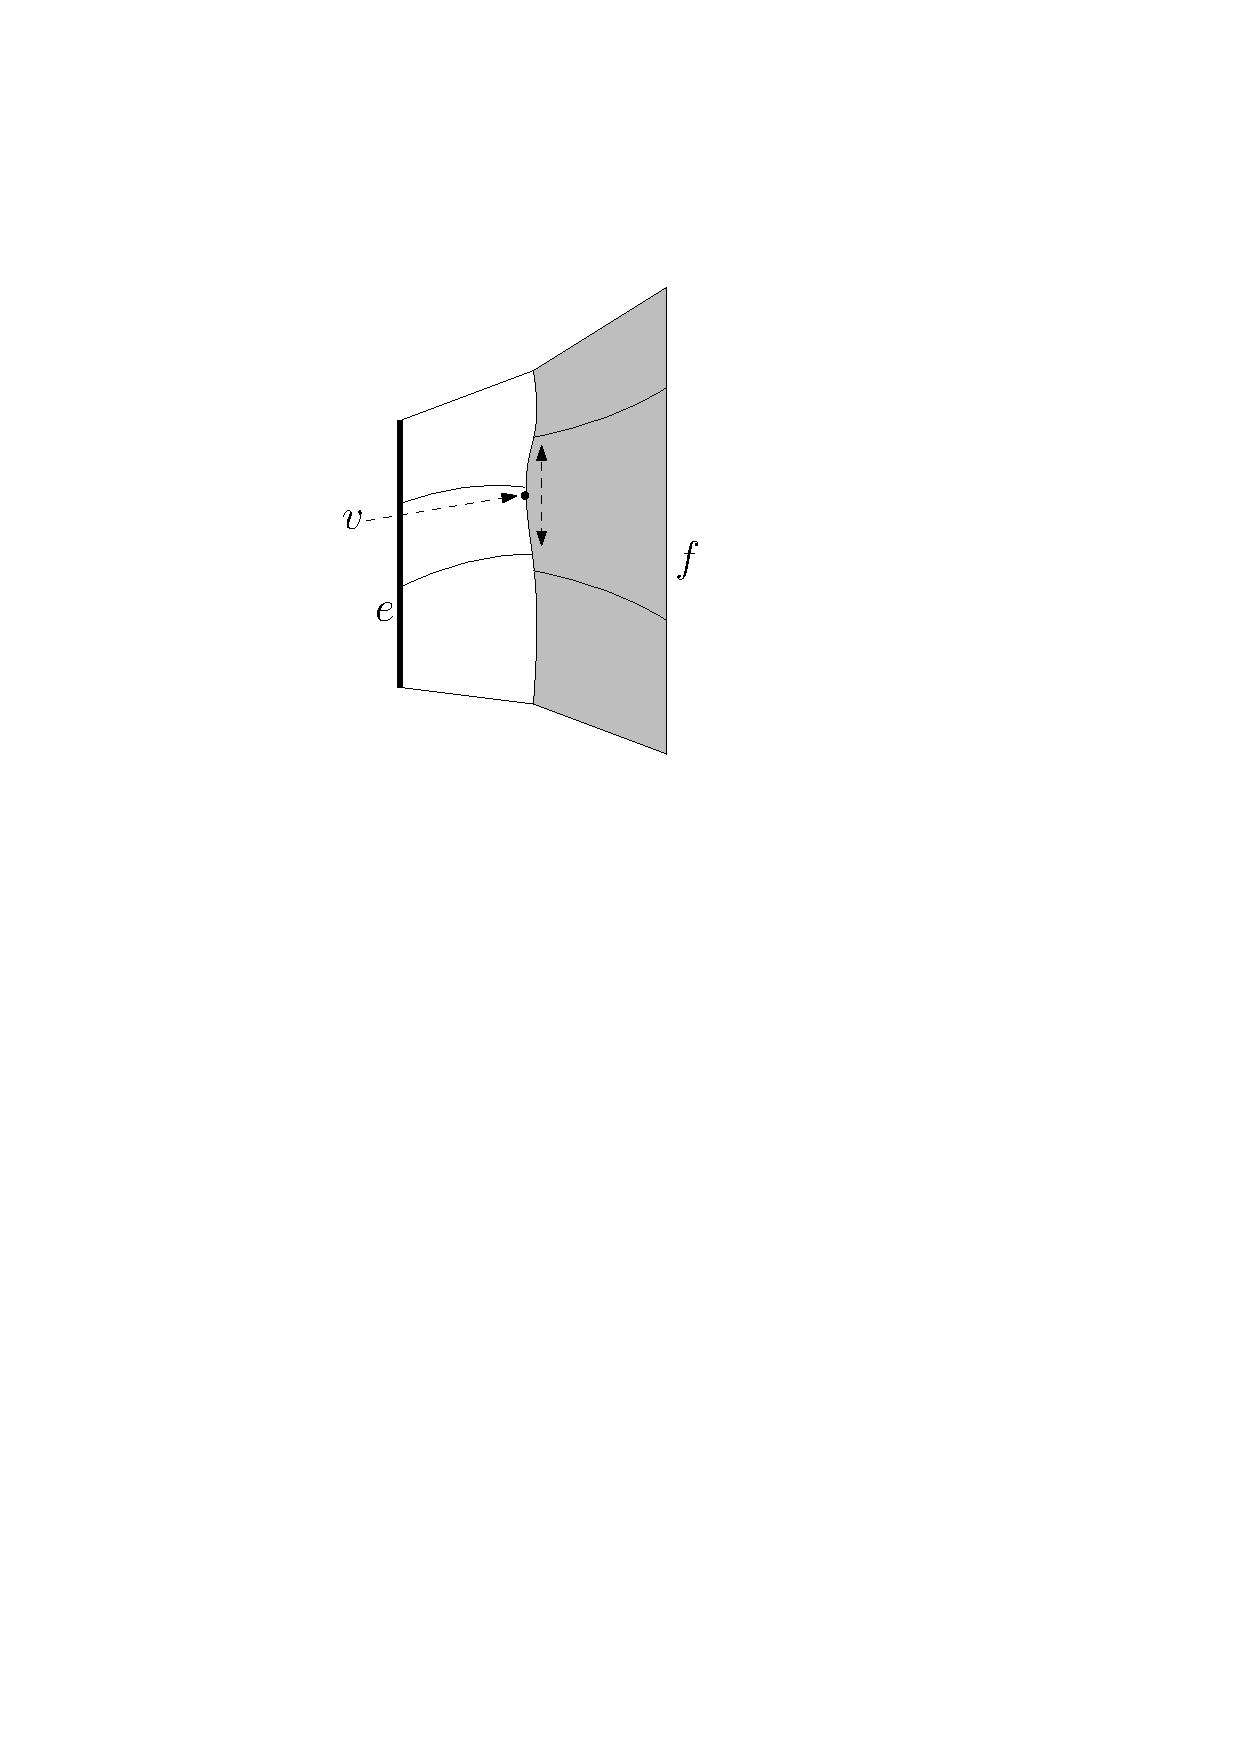
\includegraphics[width=0.35\textwidth]{figures/traceray.pdf}
	\caption{To find the region close to $W(e)$ than to $W(f)$ under weighted distance, 
    		 trace a ray from some $v \in W(e)$ through $S(e)$ and $S(f)$ until it hits a point 
             equidistant from the two wavefronts, then trace outward from the point along the bisector 
             $\Gamma$}
	\label{fig:traceray}
\end{figure}
    
    The tracing procedure computes region closer to
	$W(e)$ than to $W(f)$ for one edge $f$. Intersecting the results for all
	such edges $f$ on the boundary of the active region produces the region
	$R(e)$ claimed by $W(e)$ in $SPM(s)$. Intersecting $R(e)$ with $S(e)$ gives
	vertices of $SPM(s)$ to which $W(e)$ contributes. We repeat this computation
	for each transparent edge fragment to find all the vertices of $SPM(s)$ in
	%side 26
	the active region. Applying this algorithm to all active regions finds all
	vertices of $SPM(s)$ inside $c$.

	The partition $S(e)$ determined by each edge fragment $e$ participates $O(1)$
	times in a Voronoi-style merge, so the total cost of merging is $O(g)$.
	Hence the running time is dominated by the propagation algorithm which takes
	$O(g\log g)$ times altogether.
\end{proof}
\begin{Lemma}[Lemma 4.13 in \cite{HershbergerS99}] \label{lemma:4.13} 
	The shortest path map vertices computed cell-by-cell can be combined to
	build $SPM(s)$ in additional $O(n\log n)$	 time.
\end{Lemma}
\begin{proof}
	To compute $SPM(s)$ we compute all its edges separately then use a standard
	plane sweep to assemble them as follows. Create a list of the bisector
	endpoints discovered in the computation of Lemma \ref{lemma:4.12}, each identified by a
	key consisting of two generators. Put each three-bisector endpoint into the
	list three times, once for each bisector. Put each bisector/edge collision
	in once labeled with the generators of the bisector. Now sort the list to
	group together endpoints belonging to each bisector. Take the endpoints
	belonging to the bisector of a generator pair $(v,w)$ and sort them along
	the hyperbola determined by the weighted generators of $v$ and $w$. This
	determines all edges of $SPM(s)$ on the hyperbola. Doing this for all pairs
	that appear as keys in the sorted list gives all $O(n)$ hyperbolic arcs of
	$SPM(s)$. Finally with a standard plane sweep, we can combine these arcs
	with the edges of $\mathcal{O}$ to build the subdivision $SPM(s)$.
\end{proof}

\section{The list based data structure for wavefront propagation} \label{section:datastructurewavefront}

To keep track of our approximate wavefront, we use a list to keep track of the generators coming from 
obstacle vertices. For this list we need a data structure which supports two types of operations:

\begin{enumerate}
\item \textit{Standard list operations:} these are insert, delete, concatenate, split, find previous 
			  and next element, and search. Here the search operation locates the position of a query 
              point. This position is found in the list of bisectors defined by the generators 
              wavefront at a particular time. 
\item \textit{Priority queue operations:} these operations are used on the generators, to which we 
			  assign a priority. The data structure should be able to  update priorities and find the 
              minimum priority in the list.
\end{enumerate}

These two types of operations should be implemented in a flavor of self balancing binary trees. One 
could implement the operations e.g.\ in a red and black search tree\cite{IntroToAlg}. Here the generators will be located at the 
leaves, and each node should have a priority field which records the minimum priority of the leaves in 
it subtree.

The only requirements to the flavor of self balancing binary tree is the list operations should each 
take $O(\log n)$ time to process on a list of length $O(n)$. Each priority operation should likewise 
take $O(\log n)$ time each. 

Beside these operations we also need the tree to be fully persistent, s.t. we can operate on past 
version of any list. Each kind of operation uses $O(1)$ storage per node of the binary tree, which 
mean we can make the data structure fully persistent by path copying. The effect of using an operation 
affects $O(\log n)$ nodes of the tree, which also includes the ancestors of every affected node. We 
simple, before an operation modifies the tree, copy all the nodes that will be affected, and then
modify the copies. This way we create a new version of the tree while leaving the old version unchanged.
Since the data structure uses $O(\log n)$ for each operation, and we save a copy of size $O(\log n)$, 
the total storage usage of the data structure is $O(m \log n)$ where $m$ is total number of operations 
used. The above gives us the following lemma:

\begin{Lemma} [Lemma 5.1 in \cite{HershbergerS99}]
There is a linear-space data structure that represents an approximate wavefront an supports list 
operations and priority queue operations in $O(\log n)$ time per operation. The data structure can be 
made fully persistent at the expense of an additional $O(\log n)$ space per operation.
\end{Lemma}

\section{An implementation of the wavefront propagation} \label{section:implwavefront}

Concretely the idea of wavefront propagation is to propagate an approximate wavefront from an edge on 
the boundary of the cell containing the edge we want to propagate to. In particular, we want to propagate 
the wavefront $W(e)$, and compute $W(e,g)$ for every edge $g \in output(e)$, and in this process, assign the 
time (weight) of first contact between $W(e,g)$ and the endpoints of $g$. In this section we will show how 
to do this computation of $W(e,g)$ for all transparent edges $g$ on the boundary of $e$'s cell. 

We know from lemma \ref{lemma:4.1} that there is a constant number of edges in $output(e)$, which means 
they can only belong to a constant number of different cells. We will use this fact to compute $W(e,g)$ 
for all $g \in output(e)$. When propagating the wavefront cell-by-cell, one can think of this as splitting 
the wavefront $W(e,g)$ into multiple piece. Each piece is labeled by the sequence of crossings of the
transparent edges it follows from $e$ to $g$. The $W(e,g)$ is then made of these components wavefronts by 
concatenating the piece that are topological equivalent paths inside $\mathcal{U}(e)$. 

Since each of these component wavefronts is a list of generators, we may find that adjacent wavefront 
piece can contain duplicate generator that claims the common endpoint. One of these duplicates are to be 
deleted before the lists are concatenated.

As an example of the above see figure \ref{fig:weg}. Here $W(e,g)$ is assembled from $W(e',g)$ and 
$W(e'',g)$, where $e'$ and $e''$ are two edges on the boundary of $g$'s cell.

\begin{figure}[H]
	\centering
	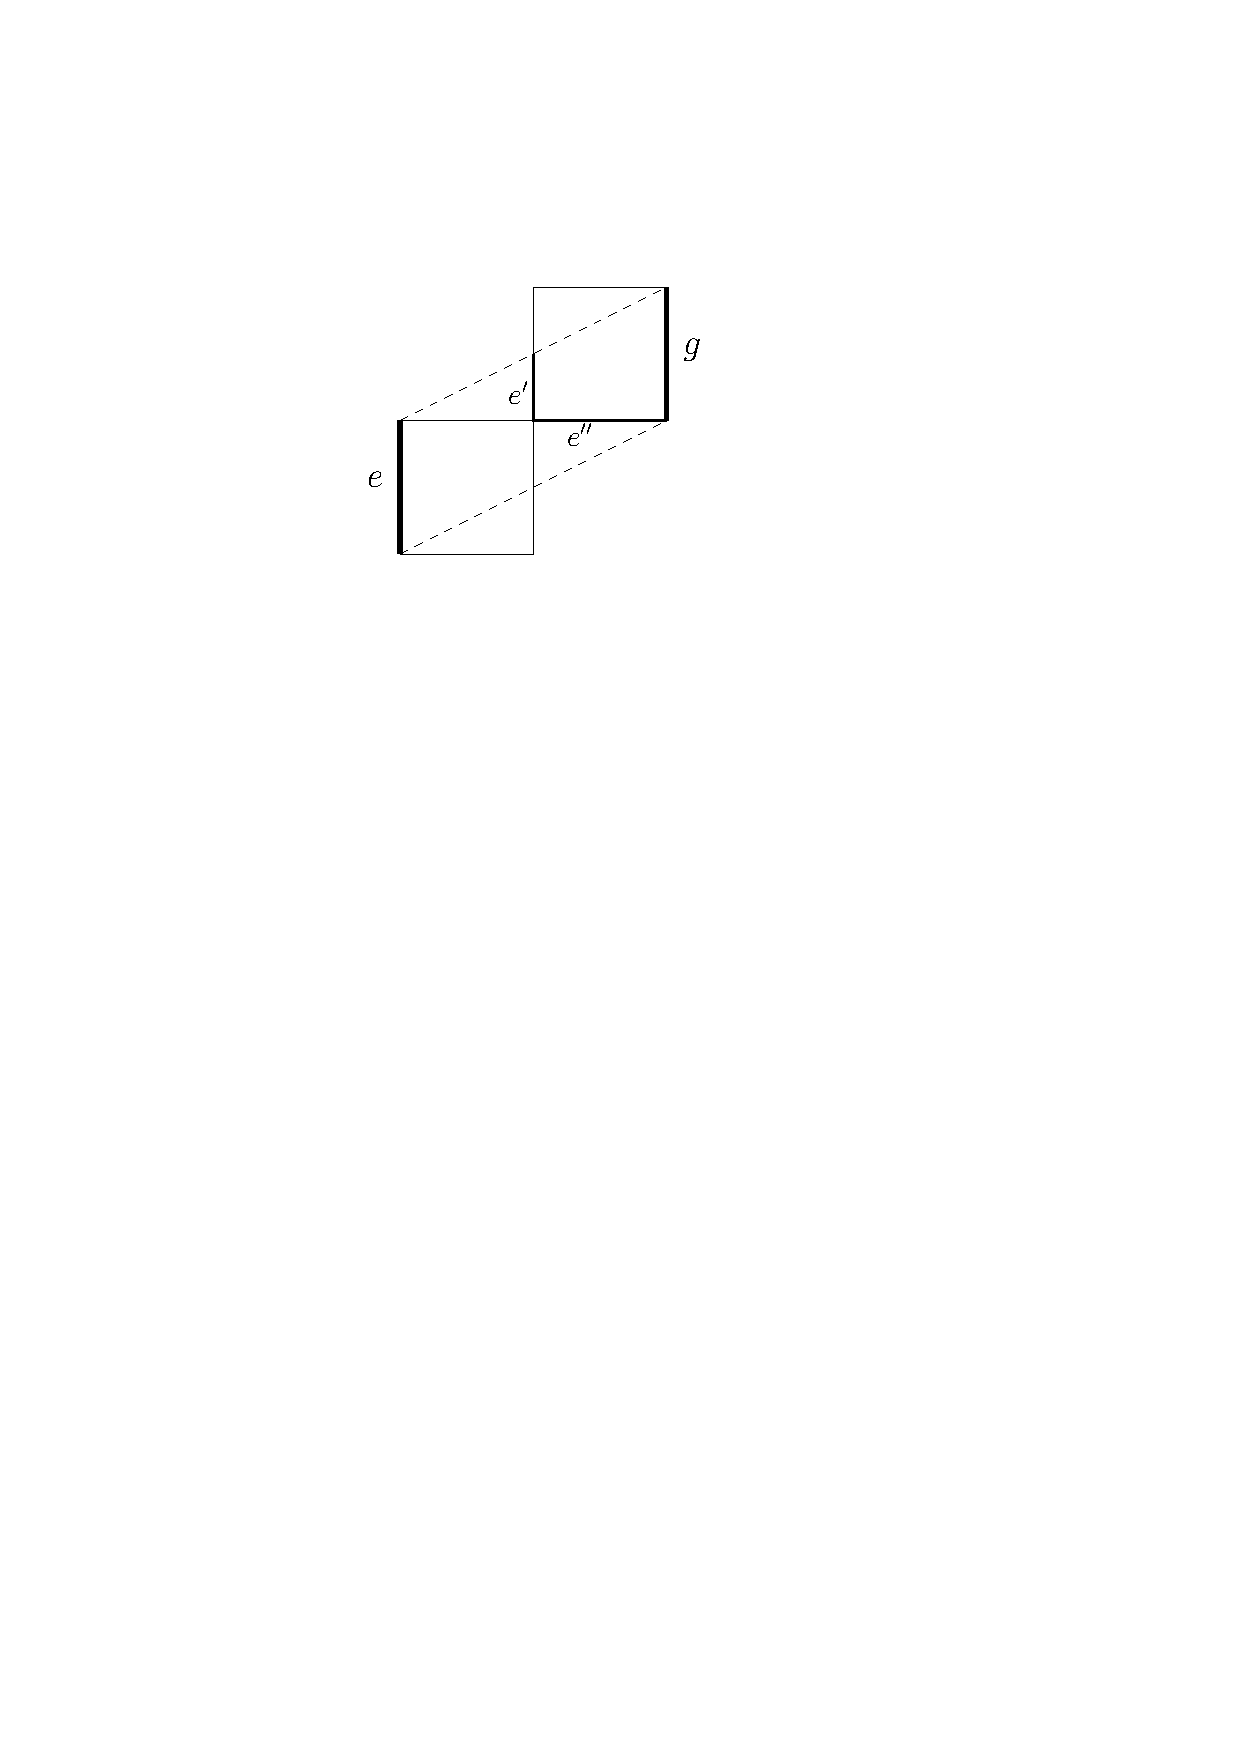
\includegraphics[width=0.4\textwidth]{figures/weg.pdf}
	\caption{$W(e,g)$ is assembled from $W(e',g)$ and $W(e'',g)$, where $e'$ and $e''$ are two edges on 
    		 the boundary of $g$'s cell\cite{HershbergerS99}.}
	\label{fig:weg}
\end{figure}

The propagation algorithm assumes that each cell $c$ is convex. Since we assumed the 
conforming subdivision could be build with square annulus's, this isn't satisfied immediately. For this we 
temporarily break a cell which isn't convex into subcells by adding transparent edges, which are 
\textit{parallel to $e$} through the points of nonconvexity. An example of this i shown in figure 
\ref{fig:preparingcells}.

\begin{figure}[H]
	\centering
	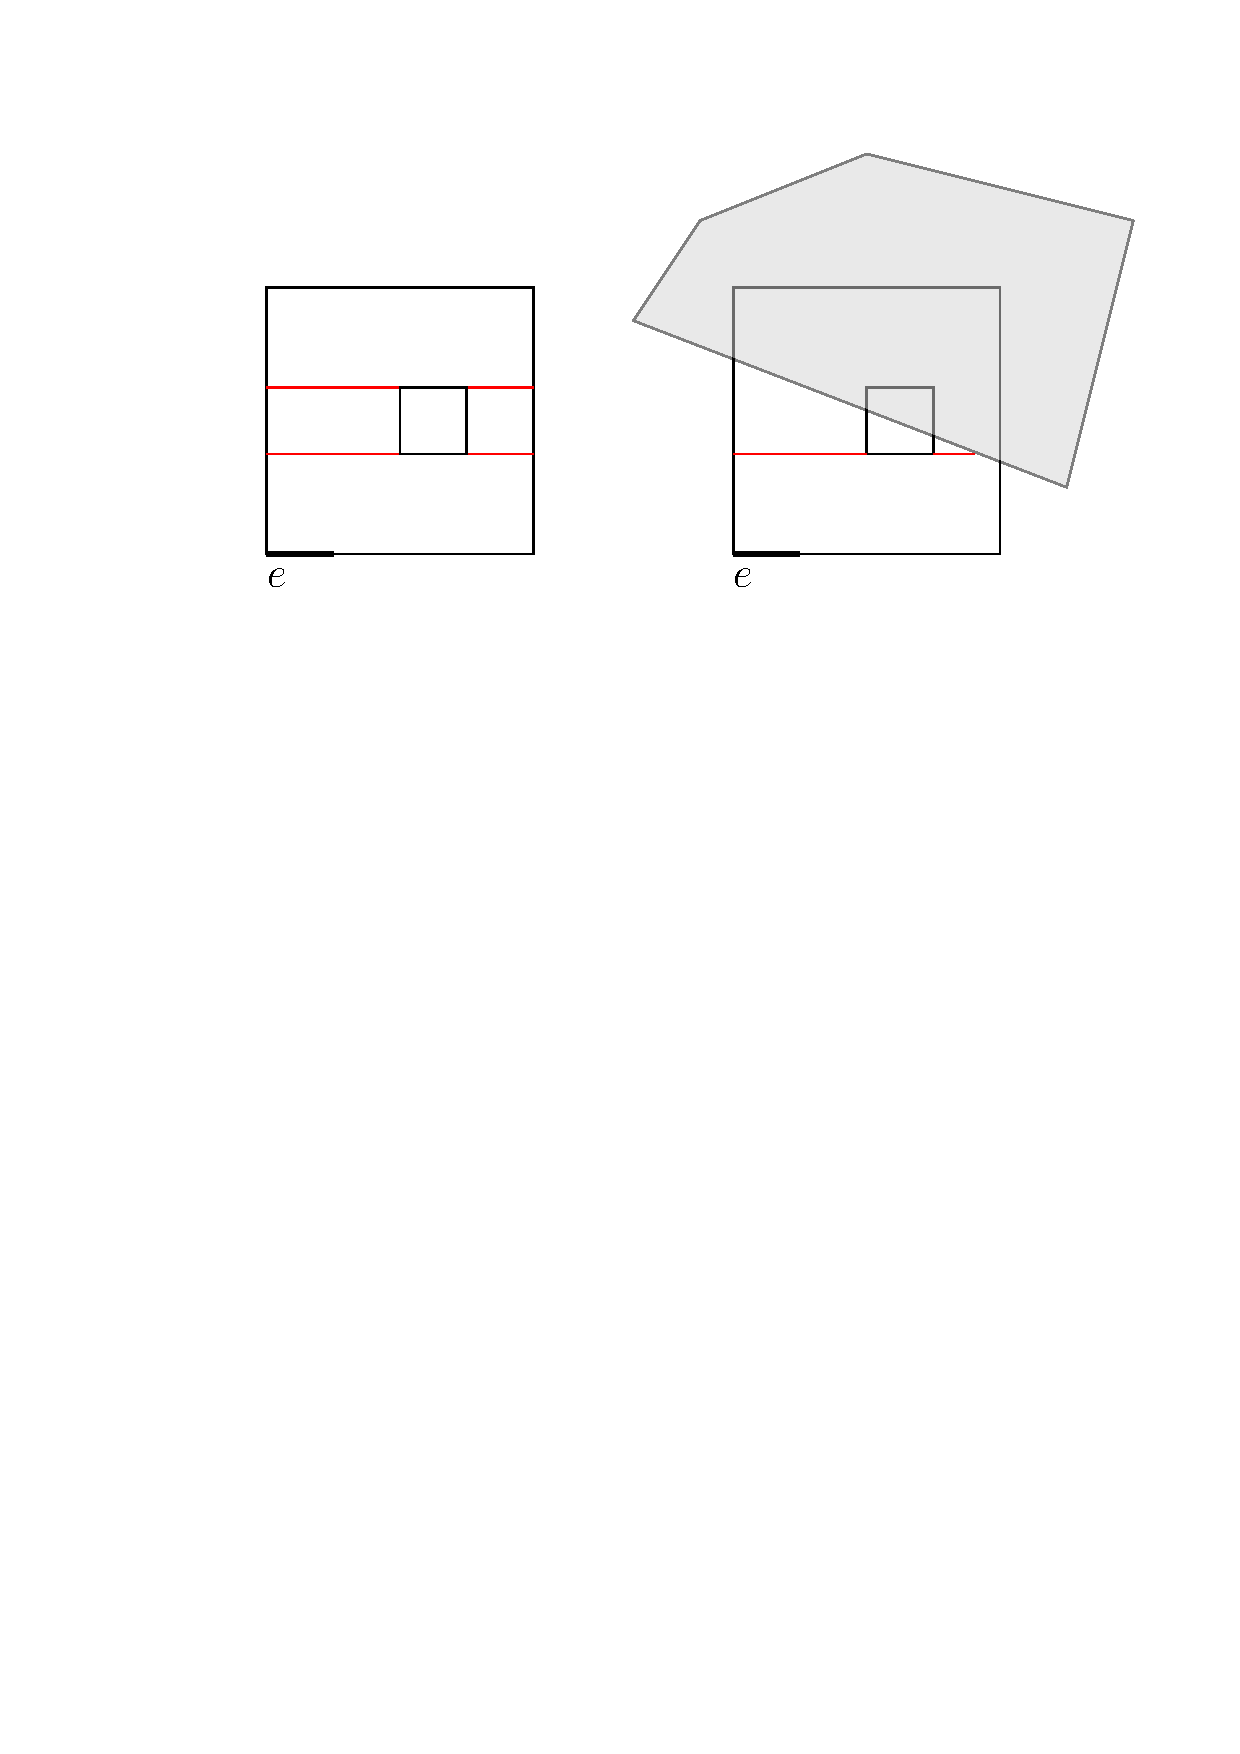
\includegraphics[width=0.7\textwidth]{figures/preparingcells.pdf}
	\caption{Insertion of transparent edges parallel to $e$ to fix the cells non convexity. The right 
    		 figure is the cases of an obstacle overlaying the cell\cite{HershbergerS99}.}
	\label{fig:preparingcells}
\end{figure}

Let $f$ be a transparent edge of the boundary of $c$ such that $f \neq e$. Then the propagation algorithm has 
the following invariant.

\paragraph{Propagation Invariant:} When a wavefront $W(e,f)$ is propagated for distance $2 \cdot | f |$
           beyond $f$, it intersects only a constant number of cells of the conforming subdivision 
           of the free space.  \\

We already saw in the former chapter that the conforming subdivision $S'$ already satisfy the Propagation 
Invariant, since, by the propagation invariant, each edge $f$ is well-covered with parameter 2. But since we 
just added some temporary transparent edges to non convex cells, we need to fix these in a way that abides to 
this invariant. This is done by dividing these added edges into $O(1)$ pieces, each no longer than the edges 
of $\mathcal{S}$ on the boundary of the annulus's outer boundary, one-eight the side length of the outer 
square, which we know is bounded by the minimum clearance property and uniform edge property of the conforming 
subdivision. These are explained in section \ref{section:def-well-covering-if-regions}. 

We now let $H$ denote the convex of $e$ and the inner square of the annulus as shown in figure 
\ref{fig:subdividedconvexhull}. A convex hull is the smallest set of points which makes the set convex \cite{CompGeo}.  
Should $H$ intersect an added transparent edge $f$, we further subdivide the 
edge segment $f \cap H$ into pieces of length equal to the inner square of the annulus, as also shown on figure 
\ref{fig:subdividedconvexhull}. 

\begin{figure}[H]
	\centering
	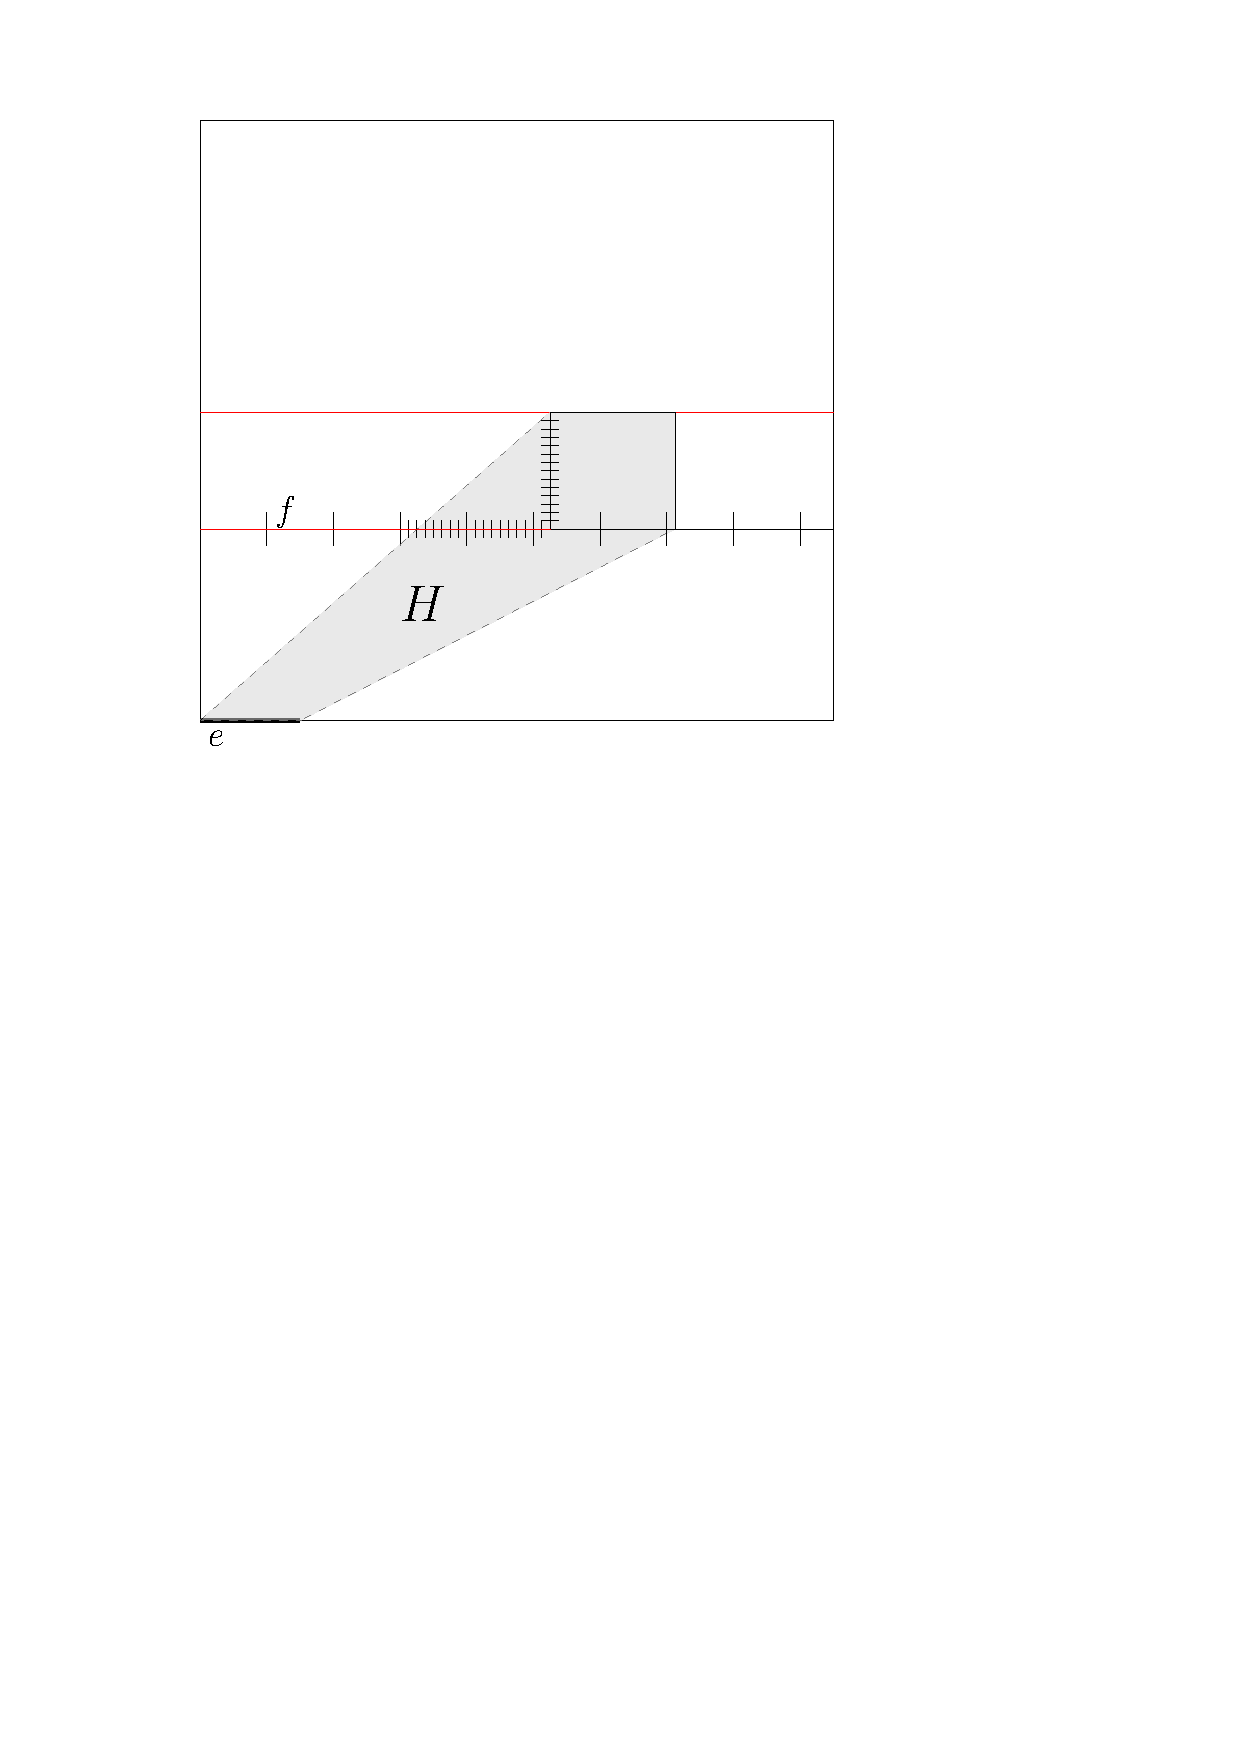
\includegraphics[width=0.6\textwidth]{figures/subdividedconvexhull.pdf}
	\caption{A subdivision of a cell, with a convex hull around a boundary edge $e$ and the inner square of 
    		 the annulus.}
	\label{fig:subdividedconvexhull}
\end{figure}

Due to $f$ being parallel with edge $e$ and the inner boundary of the annulus being well separated from the
outer boundary (see again the minimum clearance property) the total length of $f$'s edge segment inside $H$ is 
proportional to the side length of the inner square. By this it follows that the partition of $f$ only creates 
$O(1)$ edges. We can see that these subdivided edges satisfy the propagation invariant, by the following example. 
Given any such $f$, let $g'$ be an edge of $c$ such $W(e,f)$ leaves $c$ by passing through $g'$. Since $g'$ is an 
edge from the conforming subdivision of the free space, $\mathcal{S}'$, we know it is a fragment of an edge $g$ in 
the conforming subdivision of the obstacles vertices and $s$, $\mathcal{S}$. We know we from lemma 
\ref{lemma:admitsa2conformingsubdivision} (see appendix \ref{appendix:proofs}) that there are $O(1)$ cells of $S'$ 
within shortest path distance $2|g|$ 
of $g'$ by construction. Since the new transparent edge which makes the cell $c$ convex is subdivided into piece 
such that $|f| \leq |g|$, then this implies that the propagation invariant holds for the edge $f$.

\subsection{Dynamic wavefront propagation} \label{section:dynamicwavefront}

Up until now we have, in this chapter, kept the simulation of wavefront propagation rather static, in the sense that
we have look at the atomic examples of how to handle different cases at different time in the propagation process.
Now we take these ideas and see what happens when we let them operate in a dynamic setting. This means e.g. 
since a wavefront is a collection of generators, which one of the generators waves do we calculate first, and how do
we drop a generator when it has served its purpose, and so on. So we see what happens to the wavefront propagation 
when we add the element of time to the process.

So what happens to the combinatorical structure of the wavefront as it sweeps across the (convex) cells, and how 
does the wavefront $W(e)$ behave as it sweeps across a cell $c$ after entering it through the edge $e$? The 
simulation should detect and process each bisector event involving the generators from each wavefront, e.g. 
$W(e)$ that may occur inside $c$. The events are processed in an order of increasing distance to $s$. This is to 
simulate the element of time since the weight and therefore the distance to each generator is assigned by the 
arrival of the wavefront in unit speed, so distance and time are equivalent in this sense. So generator marked as 
event are process.

Let $W$ denote the current wavefront we currently are simulating, at any time in its simulation process. In the 
beginning of the simulation we have $W = W(e)$ as the approximate wavefront which passes through $e$ to compute cell
$c$. It might be the case that the edge $e$ is claimed by multiple waves, and therefore $W$ is a list of generators,
each claiming a portion of $e$. Every generator $v \in W$ defines a pair of bisectors with its neighbors in the 
list. If we let $v$ be the first generator in the list, then $v$ claims one of the endpoints of $e$, and its first 
bisector represented as the ray from $v$ through the end point of $e$. We define the last generator $v'$ 
of the generators similarly. Should $v = v'$ and claim the whole edge $e$, then there are no bisectors in the list, and the 
wave is the ray propagated from the generator through $e$. See figures \ref{fig:vandvprimesharingedge}, \ref{fig:vandvprimeallofe} and \ref{fig:visallofe}.

\begin{figure}[H]
	\caption{Crossing of two line segments}
	\minipage{0.48\textwidth}
		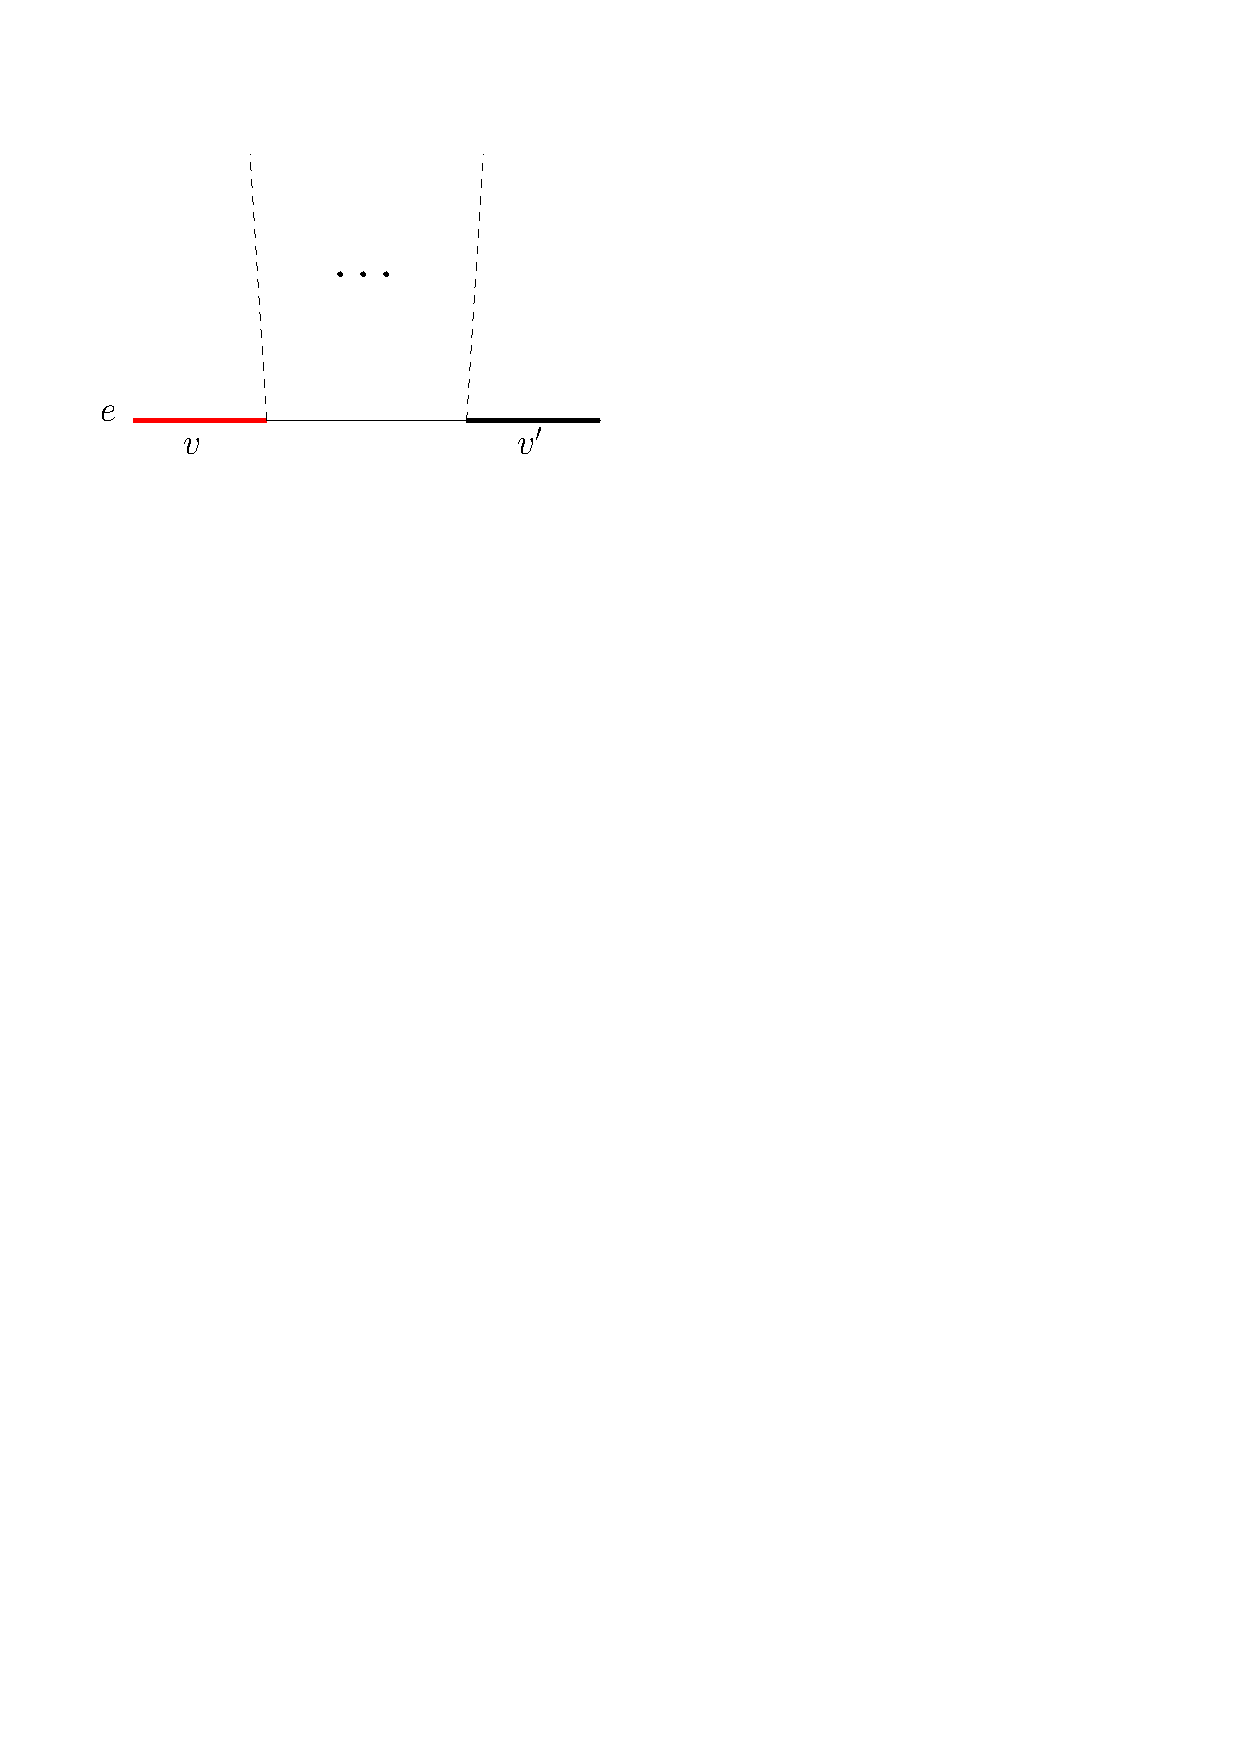
\includegraphics[height=3cm]{figures/vandvprimesharingedge.pdf}
		\caption{$v$ and $v'$ each claim the end points of $e$, with their bisectors being shared with other generators claiming the middle part of $e$, represented by the dots.}
		\label{fig:vandvprimesharingedge}
	\endminipage\hfill
	\minipage{0.48\textwidth}
		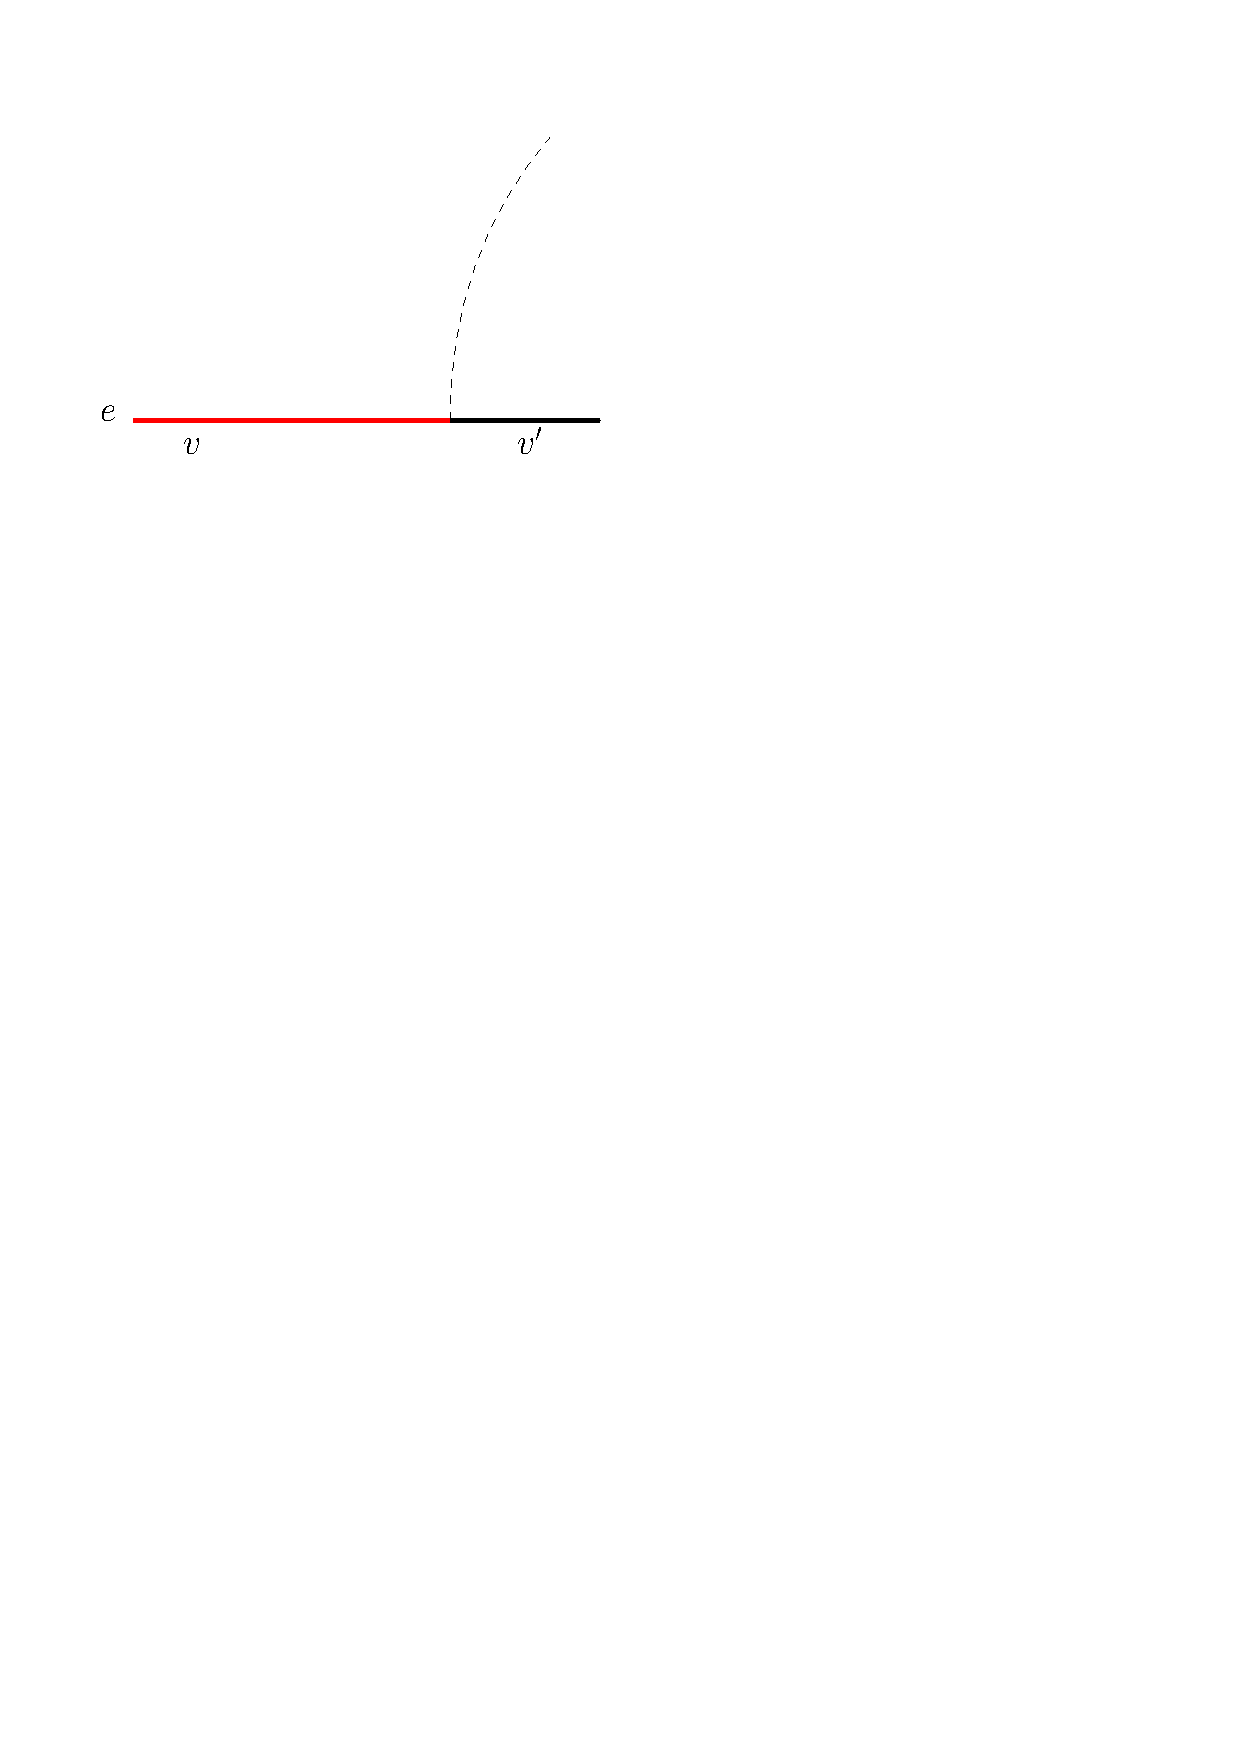
\includegraphics[height=3cm]{figures/vandvprimeallofe.pdf}
		\caption{$v$ and $v'$ claim all of $e$ and only have one bisector between them}
		\label{fig:vandvprimeallofe}
	\endminipage\hfill
	\centering
	\minipage{0.5\textwidth}
		\includegraphics[height=3cm]{figures/visallofe.pdf}
		\caption{$v$ claims all of $e$ and there are therefore no bisectors other than the ray projected from $v$ through $e$.}
		\label{fig:visallofe}
		\endminipage\hfill
\end{figure}

In order to process the bisectors event in the correct order, we will maintain the generators of $W$ in the priority queue which was 
describe in section \ref{section:datastructurewavefront}. The priority field which each node of the priority queue tree has, is 
assigned with its weighted distance to the point at which the two bisectors that defines $v$ and its neighbors intersect, beyond $e$. 
An example of this is given in figure \ref{fig:priorityvalue}. Here the bisectors defining $v$ and its neighbours intersects after 
passing through $e$, and meeting at the point $p$. This means that $v$'s priority value $priority(v) = d(s,v) + |\overline{vp}|$.

\begin{figure}[H]
	\centering
	\includegraphics[width=0.8\textwidth]{figures/priorityvalue.pdf}
	\caption{A visualization of what a generator $v$'s priority value, $|\overline{vp}| + d(s,v)$, could be with the
	         dashed lines being bisectors of the generators claiming $e$.}
	\label{fig:priorityvalue}
\end{figure}

The processing of the approximate wavefront propagation will be done in event of increasing priority up to some maximum priority 
$t_{stop}$. The $t_{stop}$ is calculated from the shape of the cell $c$, rules for this will be presented later in this section. 
The limit of $t_{stop}$ is calculated from the individual values of $t_{stop}(f)$ for each transparent edge $f$ of $c$. Initially
the values for all $f$ is $t_{stop}(f) = \infty$ and therefore $t_{stop} = \infty$. Also to keep track of the priorities through 
out the simulation, we initialize an empty set $T$ which will be cleared after each simulation.

At each step of the simulation, the generator $v$ with the lowest priority from the queue is processed, where one of following 
scenarios can happen.

\begin{enumerate}
    \item  If the event (the intersection of the $v$'s bisectors) happens inside the cell $c$, then $v$ is deleted, since it can no 
           longer propagates the free space, and we recompute the priorities for $v$'s neighbours. We mark $v$ in $W(e)$ for the cell 
           $c$ by the marking rules explained in section \ref{section:bisectorevents}, which also implies marking it in $O(1)$ number 
           of neighbouring cells to $c$ accord to the marking rules.
    \item If $v$'s event happens outside $c$, then we set $priority(v) = \infty$ and add $v$ to the set $T$. In this case the generator
          list is not changed since $v$ still has more free space outside of $c$ to propagate.
\end{enumerate}

If we where to process each bisector event of $W$ in their initialize time order, and not update them in the first of the above cases, 
then the neighboring generators of $v$ could participate in bisector event outside of cell $c$ before all bisector events inside $c$ 
were fully processed. 

So far we have seen the intersection of $v$'s bisectors if its neighbours engulfs $v$, as seen in figure \ref{fig:priorityvalue}, in 
which case we would mark $v$ by rule 3 of the generator marking rules. But it's also important to be aware that the bisector event or 
$v$ could also happen if either the intersection lies on a opaque edge of if they lie on different transparent edges with an opaque 
edge between them. In that case rule 1 above, should still do as stated, but would use rule 4 to mark $v$ for cell $c$ and its 
neighbours. Should the intersection point $p$ lie on a transparent edge, e.g. $f$, then we update our $t_{stop}$'s as follows:

\begin{align*}
    t_{stop}(f) &= \min(t_{stop}(f), d(s,v) + |\overline{vp}| + |f|) \\
    t_{stop}    &= \min(t_{stop}, t_{stop}(f))
\end{align*}

The update of $t_{stop}(f)$ is either the current $t_{stop}(f)$ or the weight as calculated the same way as in figure 
\ref{fig:priorityvalue} plus the length of the transparent edge $f$. This way we assure, that overestimate the priority 
since we would have swept all of $f$. By doing it this way, we also don't overshoot the estimate since it is still not 
$2\cdot|f|$ times greater than the time at which $W$ first comes to contact with $f$.

The $t_{stop}$ priority, which is in the priority queue, is either $t_{stop} = \infty$ in which case all events inside $c$ have been 
processed, or $t_{stop} < \infty$, which happens in the above update if there is a transparent edge $f$ on the boundary of $c$ with 
$t_{stop} = t_{stop}(f)$. We see that by updating $t_{stop}(f)$ this way, we ensure that all bisector events needed to produce $W(e,f)$
have indeed been processed. So now we move one to explain how to process $W(e,f)$. The wavefront $W(e,f)$ is calculated from $W$ in the
following way. First we locate the endpoints of $f$ in $W$, which can be done by can picking a bisector in $W$, and following its 
neighbors outwards, there is at least on such bisector (in the case of one, this bisector claims all of f). Mark the endpoint claiming 
generators by rule 2. From here we split the generator list into 3 parts. Those generators whose bisectors are between the two endpoint
claiming generators. Those are the one who will go through $f$, which after the reset of priorities will be the $W(e,f)$ wavefront, and
the other two sets are those who pass left and those who pass right of $f$, see figurue \ref{fig:wef}. The simulation process continues
with the left and right passing sets independently after the $t_{stop}$ has been reset in each set to be the minimum of $t_{stop}(g)$ 
over the transparent edges $g$ for that group. 

\begin{figure}[H]
	\centering
	\includegraphics[width=0.8\textwidth]{figures/wef.pdf}
	\caption{A visualisation of the three groups of bisectors that can occur in the calculation of $W(e,f)$. One going left of $f$, one
	         going right of $f$ (these two groups are marked with gray) and the middle group which is the group $W(e,f)$ consists of.}
	\label{fig:wef}
\end{figure}

So the above is the case of $t_{stop} < \infty$. Should we stop because we reach $t_{stop}$ and $t_{stop} = \infty$ then we split the 
current generator list at all the transparent edge endpoints, which will produce $W(e,f)$ for each transparent edge $f$, and some 
wavefront pieces that hit only opaque edges.

Should no transparent edges remain in some piece, then all bisectors in the piece hits an opaque edge, in which case we mark all the 
generators in that piece for cell $c$ and a $O(1)$ of neighboring cell by marking rule 4. We also make the necessary marking of rule 2 
and rule 3.

When finished the priority of each vertex in $T$ is reset, based on the bisectors it defines with its neighbours in the new list. This 
is done to ensure each wavefront fragment $W(e,f)$ has the proper priorities. Now we have computer $W(e,f)$ and we can determine the 
time the wavefront first makes contact, which is $d(s,v)+|\overline{vp}|$.

\subsection{Analysis of the wavefront propagation}

The propagation algorithm calls the self balancing binary priority queue $O(1)$ times with priority and list operations per bisector 
event processed and $O(1)$ for each edge in the conforming subdivision (transparent edge). Each operation takes by construction of the 
data structure $O(\log n)$ time and space. Since the data structure by construction is fully persistent, all the modifications we 
do when computing a single wavefront list $W(e)$ are independent.

The main result for section \ref{section:dynamicwavefront} can be summarized in the following lemma:

\begin{Lemma} [Lemma 5.2 in \cite{HershbergerS99}]
Every bisector event processed in the procedure described in section \ref{section:dynamicwavefront} either:
\begin{enumerate}
    \item Lies inside cell $c$.
    \item Involves a generator whose region is truncated by an opaque edge of $c$.
    \item Is associated with $t_{stop}(f)$ being set to a finite value for the first time for some transparent edge $f$ of $c$, or
    \item Lies within shortest path distance $2\cdot|f|$ of a transparent edge $f$ of $c$. 
\end{enumerate}
If the number of event is $m$, then the procedure takes $O(m \log n)$ time.
\end{Lemma}

This Lemma, together with the results of chapter \ref{chapter:shortestpathmap} and \ref{chapter:conformingsubdivision} gives us the 
following theorem due to Hershberger and Suri \cite{HershbergerS99}.

\begin{theorem}[Theorem 5.3 in \cite{HershbergerS99}]
Let $\mathcal{O}$ be a family of polygonal obstacles in the plane with pairwise disjoint interiors and a total of $n$ vertices. Given a
point $s$, we can construct the shortest path map from $s$ with respect to $\mathcal{O}$ in time $O(n \log n)$ and space $O(n \log n)$.
\end{theorem}

By this theorem we see that, one can compute the $SPM(s)$ by processing the point locations in the plane, where after 
one can make a shortest path query from $s$ to any point $t$ in the plane, which can be answered in time $O(\log n)$ 
due to \cite{DBLP:journals/siamcomp/Kirkpatrick83}. A shortest path $\pi(s,t)$ can be computed in additional $O(h)$ 
time, where $h$ is the number of edges in $\pi(s,t)$.




\chapter{Algorithm for shortest path with obstacle violations}

\section{Overview of $SPM_k$}

We begin this chapter by given a formal definition of $SPM$ and $SPM_k$.

\begin{mydef}
	\textbf{Shortest Path Map:} \\ 
	The shortest path map  of a
	particular source point s, denoted $SPM(s)$, is a subdivision of the plane
	into two-dimensional regions such that all the points in one region have the
	same, unique predecessor\cite{HershbergerS99}. In the case legal obstacle
	violations we use a shortest path map with k violations denoted by
	$SPM_k(p)$. This map has a fixed source and contains the set of unique
	shortest paths from $s$ to $p$, one for each number of violation we allow
	from $0,1,...,k$. 
\end{mydef}



\section{Algorithm for constructing $SPM_k$}

This section is dedicated to showing the extension of the Hershberger Suri algorithm which was presented in chapter 
\ref{chapter:conformingsubdivision} and \ref{chapter:shortestpathmap} for calculating a shortest $k$-path map, $SPM_k$ in time $O(k^2 \cdot 
n \log n)$. This is done by extending this continuous Dijkstra method into a $k$-garage structure. This way we can enter each level $i$ by 
going through an obstacle polygon in level $i-1$, and leave it into the next layer $i$. This can then be done up to $k$ times, which is 
equivalent to violating $k$ obstacles. So more precisely, when a wavefront hit an obstacle $O \in \mathcal{O}$, it claims the sub edges of 
the outer boundary of $O$, and then is re emitted into the interior of $O$, therefore also claiming the interior space of $O$. When reaching
the opposite side of $O$ from which it entered, it is re emitted into the free space free space a level higher than when entering. Therefore
this "vertical" movement in the interior of $O$ adds no time delay. So in this extension a wavefront at time $T$ contains all points at all 
levels which has $T$ distance to $s$. 

Another change has to be made to the Hershberger Suri algorithm which involves how we identifies generators i each level. Before we had a 
generator $g$ known by which vertex $v$ it start emitting from, and the time $t$ in which it starts to emit. When using the elevator we pass
through some subedges of $O$, which leads us to define the generators in term of a triplet, which now also involves the sub edge on the 
border of $O$ through which we enter this new level, see figure \ref{fig:tripletgenerator}.

\begin{figure}[H]
	\centering
	\includegraphics[width=0.8\textwidth]{figures/tripletgenerator.pdf}
	\caption{An example of a triplet generator where $v$ starts to emit at time $t$, and enter obstacle $O$ through edge $e$, which 
	         creates the new tiples generator $(v,t,e)$. }
	\label{fig:tripletgenerator}
\end{figure}

We can now imaging that entering the next level through $e$ is the same as emitting a wave from $v$ through the interior "triangular 
flap", shown in figure \ref{fig:tripletgenerator} with dotted lines, which is connected to $e$ and from there enter the free space at the 
next floor. Algorithmically we ignore the triangular flap, and start emitting directly from $e$, which is another difference compared to 
the unmodified Hershberger Suri algorithm where we only emitted from points, and not edges. So we do the following for each edge $e$ of 
the conforming sub division, as described in \cite{HershbergerKS17}:

\begin{enumerate}
    \item Find all boundary sources $(v,t,e)$ such that the well-covering region of $\mathcal{U}(f)$ which contains $e$.
    \item Initialize $covertime(f)$, which is the time at which $f$ would be engulfed by the wavefront minimizing over all boundary 
          sources $(v,t,e)$ with $e \in \mathcal{U}(f)$ and for each such source considering paths from $v$ with delay $t$, constrained to
          pass through $e$.
    \item For each source $(v,t,e)$ with $e \in \mathcal{U}(f)$, propagate its wavelet to $e$ inside $\mathcal{U}(f)$.
\end{enumerate}

By using the modified Hershberger Suri algorithm described above we get the following lemma, which we will use with out proof.

\begin{Lemma}[Lemma 22 in \cite{HershbergerKS17}]
Given $m$ boundary sources in a polygonal domain with $n$ vertices, we can compute the exit claims of the sources in $O((m + n) \cdot \log
(m + n))$ time and space.
\end{Lemma}

New we are ready to present the algorithm for constructing the $SPM_k$. The algorithm takes as a polygon $\mathcal{P}$ which encapsulate all 
the vertices in the plane we want in our $SPM_k$. The obstacles should be convex obstacles, which is a tighter condition than the unmodified 
Hershberger Suri algorithm, which also will work for non convex obstacles. Let $M$ denote the set of boundary sources, which will be 
passed to the modified Hershberger Suri algorithm. The algorithm computes two different things, namely the $(k-1)$-visibility region $V$ 
and the $k=$-path map $SPM_{=k}$, which together forms the $SPM_k$. The length from $s$ to a point $p$ in the plane by first locating the 
region in the $SPM_k$ which contains $p$ and then follow the $k$-predecessor of the region, back to $s$  adding their length.

\begin{algorithm}[H]
	\caption{Construct $SPM_k$} \label{algorithm:constructspmk}
	\begin{algorithmic}[1]
	    \State Set $M=\{s\}$
	    \State call the Hershberger-Suri algorithm on $\mathcal{P}$ and computer $SPM_0$
	    \State Let $V = \emptyset$
		\For {$i = 1$ to $k$}
		    \State \multiline{Using the modified Hershberger-Suri algorithm propagate the sources in $SPM_{i-1}$ the 
		                      obstacles in $\mathcal{P}$ and compute the set of boundary sources $M_{new}$ for $SPM_{=i}$}
            \State \multiline{Identify all the regions in $SPM_{=(i-1)}$ for which the predecessor is $s$. Observe 
                             that this is precisely the region $V' = V_{i-1} \setminus V_{i-2}$. Set $\mathcal{P}$ to be the 
                             new polygon domain with this region removed.}
            \If {$V = \emptyset$ then}
                \State {set $V = V'$}
            \Else 
                \State {Merge $V$ with $V'$ at the common vertices.}
            \EndIf
            \State {Set $M = M_{new}$}
            \State \multiline{Call the modified Hershberger-Suri algorithm  to compute $SPM_{=i}$ for input $P$}
        \EndFor
        \State \multiline{Merge $SPM_{=k}$ with $v$ at the boundary of regions of $SPM_{=k}$ that have $s$ as predecessor, 
                          i.e. $V' = V_k \setminus V_{k-1}$ to obtain $SPM_k$}
	\end{algorithmic} 
\end{algorithm}

When end this chapter with the theorem for the running time of algorithm above

\begin{theorem} [Theorem 23 in \cite{HershbergerKS17}]
If $P$ is a polygonal domain bounded by convex obstacles with a total of $n$ vertices, the shortest $k$-path map for $P$ with respect to a srouce point $s$ can be computed in $O(k^2 \cdot n \cdot \log n)$ time and $O(k \cdot n \log n)$ space.
\end{theorem}


\chapter{Lower bound of the "shortest path in the plane with obstacles" problem}
\label{chapter:lowerbound}
In this chapter we will show the shortest path without violation has a
$\Omega{(n\log n)}$ lower bound in the algebraic computation tree model, 
and therefore affirming that the Hershberger Suri algorithm is optimal.
First we will introduce the element distinction problem, then we present a
lower bound for that problem. Afterwards we present the sorting problem, and
making a reduction to the element distinction problem and thereby showing that
sorting must have at least the same lower bound as element distinction and
lastly showing that the shortest path in the plane without violations can be
used to sort number and thereby showing that the shortest path problem has a
lower bound which is at least the same.
\section{The Algebraic Computation Tree Model}
The idea of the The Algebraic Computation Tree Model is to construct a rooted
tree where each path from the root to a leaf is a membership test.
Let $W \subseteq \mathbb{R}^n$ be any set. The membership problem for $W$ is
the following:
\begin{align}
	\text{Given } x = (x_1,\dots,x_n) \in \mathbb{R}^n \text{ determine if } x\in W
\end{align}
Formally a computation tree $T$ for each vertex $v$ it holds that
\begin{itemize}
  \item If $v$ has one son it computes one of the following computations
			\begin{align}
				f_v:=f_{v_1} \circ f_{v_2}\quad \text{ or }\quad
				f_v:=c \circ f_{v_1}\quad \text{ or }\quad
				f_v:=\sqrt{f_{v_1}}
				\label{form:computation}
			\end{align}
  	 where $v_i$ is an ancestor of $v$ in the tree $T$ or $f_{v_i}\in
  	 \{x_1,\dots,x_n\}$, $\circ \in \{+,-,\cdot,/\}$
   \item If $v$ has two children it is a test instruction on the form
		\begin{align}
			 f_{v_1}>0\quad \text{ or }\quad
			 f_{v_1}\geq 0\quad \text{ or }\quad
			 f_{v_1}= 0
			 \label{form:comparison}
		\end{align}
   \item If $v$ is a leaf it is either labeled YES or NO, depending on
  	 weather the path down the tree $T$ makes $(x_1,\dots,x_n)\in W$
\end{itemize}
So given and input $x\in \mathbb{R}^n$ we can build a tree $T$ and find the
depth of the tree to see what the lower bound of the computation is.
The impotent thing to note is that we are allowed to make comparison (formula
\ref{form:comparison}) and computation (formula \ref{form:comparison}).

\section{Element distinction problem}

The element distinctness problem is as follows
\begin{mydef} \textbf{(Element distinctness problem:)} \\
	\label{def:distinction}
	Given $n$ elements $x_1,\dots,x_n\in \mathbb{R}$ is there a pair $x_i=x_j$
	where $i\neq j$?
\end{mydef}

The following theorem is due to Michael Ben-Or 83\cite{DBLP:conf/stoc/Ben-Or83}

\begin{theorem}
	\label{thm:distinction_lower}
Any algebraic computation tree that solves the n-element distinctness problem
must have complexity of at least $\Omega{(n \log n)}$
\end{theorem}

With that settled, we will move on to sorting

\subsection{Sorting of numbers}

\begin{mydef}[Section 2.1 \cite{IntroToAlg}]\textbf{(Sorting:)} \label{def:sorting} \\
    Given a sequence of $n$ numbers $x_1,\dots,x_n$ find er permutation
	$x'_1,\dots,x'_n$ such that  $x'_1\leq x'_2 \leq\dots\leq x'_n$
\end{mydef}

Now we make a reduction from distinction definition (\ref{def:distinction}) to
sorting definition (\ref{def:sorting}). We are given $x_1,\dots, x_n$, and wants to
see if there exists a pair $x_i=x_j$ where $i\neq j$. We do this by sorting the
values and afterwards make a linear scan to see if $x'_i = x'_{i+1}$ since the 
elements is in sorted order, two element that are the same will appear next to
each other in the sorted sequence, so we will find it using this approach.
Since the reduction takes $O(n)$ and the element distinction can be solved
using sorting that means that sorting must have at least the same lower bound,
$\Omega(n\log n)$, as element distinction. 

\subsection{Shortest path in the plane}
Now we make a reduction from sorting numbers to calculating the shortest path
in the plane with obstacles (See section \ref{problemdescription} for the
formal definition).
Given numbers $x_1,\dots,x_n\in \mathbb{N}$, and lets for simplicity say they are all positive
(i.e.\ $x_i>0$ for $i=1,\dots,n$) we construct the obstacle as follows: Take each
point $x_i$ and construct a rectangle with the following points
$(x_i,x_i^2),(x_i-1,x_i^2),(x_i-1,\max), (x_i,\max)$, where max is the maximum
value (see Figure \ref{fig:reduction})

\begin{figure}[H]
	\includegraphics{figures/reduction.pdf}
	\caption{An example of the reduction from sorting numbers to shortest path}
	\label{fig:reduction}
\end{figure}

Set $s=(0,0)$ and let
$i_{max}=\underset{i}{\arg\max}(x_i)$ and set $t=(x_{i_{max}},x_{i_{max}}^2)$.
This gives us a an instance of shortest path problem in the plane with obstacles where
each rectangle which lower right corner lies on the
function $f(x)=x^2$, this function is convex which results in every rectangles
lower right corner being visited on the way from $s$ to $t$. Now we can run our
SPM algorithm, get out a path which will be the sorted range of the numbers.

Given that the reduction (constructing the rectangles and finding $t$) takes
$O(n)$ we can conclude that we can make a reduction from number sorting to
finding the shortest path in the plane with obstacles. This mean that we have
shown a $\Omega{(n\log n)}$ lower bound on shortest path in the plane with obstacles.


\chapter{Conclusion}

In this thesis we have studied the problem of finding the shortest path in a plane with $k$ 
polygonal obstacle violations. First we showed a naive way for computing this problem, by 
building a visibility graph and using Dijkstra to find the shortest path with a maximum of 
$k$ allowed obstacle violation. This could be done in $O(n^3 + k \cdot n^2 + \text{Dijkstra})$, 
where Dijkstra runs in time $O((V + E) \log V)$. We implemented our naive algorithm a found 
our implementation ran in the expected time. 

Next we present an optimal solution of solving the shortest path problem without obstacle violation, 
which is due to Hershberger and Suri\cite{HershbergerS99}, and presented an extension of this solution 
into one which could handle paths with obstacle violation, which is due to Hershberger, Kumar and Suri
\cite{HershbergerKS17}. 

We began our discussion of the Hershberger-Suri algorithm with the construction of a conforming 
subdivision which builds a grid on top of the plane which give us some strong properties for subdividing 
it into a shortest path math. Here we considered both theoretical results and implementation details. 
Next we presented the wavefront propagation which uses the conforming subdivision to construct 
the shortest path map, from which we can query the shortest path between a source point $s$ 
and an endpoint $t$ in time $O(\log n)$ \cite{DBLP:journals/siamcomp/Kirkpatrick83}. 

Next we presented the extension of the Hershberger-Suri algorithm, with the needed modification
to the Hershberger-Suri algorithm and the overall algorithm which solves the shortest path with
$k$ polygonal obstacle violations in $k^2 \cdot n \log n)$ time. We also gave an overview of the
theory behind the solution to give a better understanding of the main ideas on which the algorithm
is build upon.

At last we gave a reduction of finding a shortest path without obstacle violation to sorting numbers
and proved the optimally of the Hershberger-Suri algorithm.

\section{Future work}

\newpage

\appendix

\chapter{Definition for a hyperbola and bisection}
\label{appendix:def}
\section{Hyperbola definition} 

\begin{mydef}
	\textbf{Hyperbola:} \\ 
	A hyperbola is a set of
	points, such that for any point $P$ of the set, the absolute difference of
	the distance $|PF_1|$, $|PF_2|$ to two fixed points $F_1$, $F_2$, also known
	as the \textit{foci}, is constant, usually denoted by $2a, a>0$\cite{Hyperbola}:
	
	$$H=\{P \mid ||PF_1|-|PF_2|| = 2a\}$$ 
\end{mydef}

\begin{figure}[H] 
	\centering
	\includegraphics[width=0.65\textwidth]{figures/hyperbola.pdf} 
	\caption{Example of a hyperbola} 
	\label{fig:hyperbola} 
\end{figure}

\newpage

\section{Bisection}

\begin{mydef}
	\textbf{Bisection:} \\ 
	Bisection is the division of something into
	two equal or congruent parts, usually by a line, which is then called a
	bisector. The most often considered types of bisectors are the segment
	bisector (a line that passes through the midpoint of a given segment) and
	the angle bisector (a line that passes through the apex of an angle, that
	divides it into two equal angles).\cite{Bisector-collinearity-convexPoly}
\end{mydef}

\begin{figure}[H] 
	\centering
	\includegraphics[width=0.65\textwidth]{figures/bisector.pdf} 
	\caption{Example of Segment Bisection} 
	\label{fig:SegmentBisection} 
\end{figure}
\chapter{Delaunay triangulation}\label{appendix:delaunaykruskal}

To understand what a Delaunay triangulation is, we start by understanding what a 
Voronoi digram is. The Voronoi digram is build around points in a plane, where 
the plane partition into a set of cells, where each cell has exactly one point 
in its interior. The special property for each of these cells is that each edge 
in there border is placed between two points, in such a way that the distance 
from the two points to any point on the edge is the same. The Voronoi digram can 
be computed in $O(n \log n)$ time \cite{CompGeo}. 

Delaunay Triangulation can then be understood as the dual graph of the Voronoi 
diagram. That is, we can build a graph, where the vertex in each cell of the 
Voronoi diagram gets a edge to another vertex if the vertex is a neighboring 
cell. This gives us a triangulation of the all the points in the plane, where
no edge overlaps.
\chapter{Survival guide}

\begin{figure}
\begin{center}
    \addtolength{\leftskip} {-2.5cm} % increase (absolute) value if needed
    \addtolength{\rightskip}{-2.5cm}
\begin{tabular}{| c | l |}
	\hline
	$n$ & number of vertices \\
	\hline
	$k$ & number of violation \\
	\hline
	$l_i,l$ & edge segments \\
	\hline
	$e,e_i,f,f_i$ & edges \\
	\hline
	$i,j$ & counting variables \\
	\hline
	$p,p_i,q,q_i,a,b,r$ & points \\
	\hline
	$s$ & stars point, source \\
	\hline
	$t$ & end point \\
	\hline
	$V$ & set of vertices, in the context of $G(E,V)$, else all vertices in the plane including $s$\\
	\hline
	$E$ & set of edges \\
	\hline
	$G$ & Graph \\
	\hline
	$p_{i.x}, q_{i.x}$ & $x$ coordinate of points \\
	\hline
	$p_{i.y}, q_{i.y}$ & $4$ coordinate of points\\
	\hline
	$v_i$ & vectors or vertices \\
	\hline
	$A,B,C$ & Figures, like triangles and square, or corners of triangles \\
	\hline
	$L_i$ & lines \\
	\hline
	$v_{\pi}$ & predecessor \\
	\hline
	$s_d, v_d$ & upper bound of weight of shortest paths \\
	\hline
	$w(\cdot, \cdot), w(\cdot)$ & weight function with one or two inputs \\
	\hline
	$Q$ & min priority queue \\
	\hline
	$\mathcal{S}$ & straight line subdivision \\
	\hline
\end{tabular}
\end{center}
\end{figure}


\begin{figure}
\begin{center}
    \addtolength{\leftskip} {-2.5cm} % increase (absolute) value if needed
    \addtolength{\rightskip}{-2.5cm}
\begin{tabular}{| c | l |}
    \hline
	$\alpha$ & well covering parameter \\
	\hline
	$C(e)$ & set of cells with $e$ in its interior \\
	$\mathcal{C}_i(e_i)$ & set of cells of $\mathcal{S}_i$ whose union $\mathcal{U}_{\alpha}(e_\alpha)$ the the well covering region $e_{\alpha}$ \\ 
	\hline
	$\mathcal{U}(e)$ & $\{c \mid c \in \mathcal{C}(e)\}$ \\
	\hline
	$c$ & cell \\
    \hline
	$\Delta$ & side length of figure \\
	\hline
	$x,y$ & $= j \cdot 2^i$ coordinate of $i$-quad \\
	\hline
	$b$ & $i$-box \\
	\hline
	$\mathcal{Q}(i)$ & $i$-quads at stage $i$ \\
	\hline
	$S, S', S_j(i)$ & equivalence class of $\mathcal{Q}(i)$ \\
	\hline
	$\equiv_i$ & transitive equivalence relation of overlap \\
    \hline
	$input(e)$ & edges who's wavefront is used for computing distance to $e$ from $\mathcal{U}(e)$'s boundary \\
	\hline
	$output(e)$ & $input(e) \cup \{f \mid e \in input(f)\}$ \\
	\hline
	$\partial$ & boundary \\
	\hline
	$V_S$ & points in the cores $S$ quads \\
	\hline
	$\overline{pq}$ & line segment between point $p$ and $q$ \\
	\hline
	$covertime(e)$ & time where $e$ is fully covered \\
	\hline
	$w,w'$ & wavelet \\
	\hline
	$O, O_i$ & obstacle \\
	\hline
	$\mathcal{O}$ & the set of obstacles in the plane \\
	\hline
	$g,g'$ & generators \\
	\hline
	$\pi(p)$ & set of shortest path from $s$ to $p$ \\
	\hline
	$\pi_k(p)$ & the shortest path from $s$ to $p$ \\
	\hline
	$SPM$ & shortest path map \\
	\hline
	$SPM_k$ & shortest $k$-path map\\
	\hline
	$T, T_i$ & minimum spanning tree or subset of edges \\
	\hline
	$T'$ & joined tree of $T_1$ and $T_2$ \\
	\hline
	$T_x$ & one of $\{T_1, T_2\}$ \\
	\hline
	$\mathcal{N}$ & set of minimum spanning trees \\
	\hline
	$G(i)$ & graph with set of vertices $V$ with edges weight of less than $6 \cdot 2^i$ \\
	\hline
	$|\cdot|$ & length of edges of size of set \\
	\hline
	$R_1$ & $\bigcup_{q \in S'} \{\text{the core of } growth(q)\}$ \\
	\hline
	$R_2$ & $\bigcup_{q \in S'} \{\text{the region covered by } q\}$ \\
	\hline
	$M$ & matching in graph \\
	\hline
	$q_u, q_v$ & $i$-quad q containing vertex $v$ or $u$ in its core \\
	\hline
	$MSF(\cdot)$ & minimum spanning forest at stage $i$ \\
	\hline
	$d(\cdot, \cdot)$ & distance function \\
	\hline
	$\Tilde{d}(s,e)$ & $\min(d(s,a),d(s,b))$ \\
	\hline
	$W(e)$ & approximate wavefront passing through edge $e$ \\
	\hline
	$W(f,e)$ & $\{w(f) \mid f \in input(e)\}$ \\
	\hline
	$W(f',e)$ & topologically different than $W(f,e)$ \\
	\hline
	$S(e)$ & S-face which segment intersects $e$ \\
	\hline
	S-face & piece of active region
	\hline
\end{tabular}
\end{center}
\end{figure}
\chapter{Tables}
\begin{table}[H]
\begin{tabular}{ |c|c| } 
 \hline
	n & time (in miliseconds) \\
	\hline
	2 & 0 \\
	\hline
	6 & 0 \\
	\hline
	18 & 0 \\
	\hline
	38 & 1 \\
	\hline
	66 & 9 \\
	\hline
	102 & 24 \\
	\hline
	146 & 50 \\
	\hline
	198 & 112 \\
	\hline
	258 & 235 \\
	\hline
	326 & 466 \\
	\hline
	402 & 848 \\
	\hline
	486 & 1481 \\
	\hline
	578 & 2462 \\
	\hline
	678 & 3939 \\
	\hline
	786 & 6083 \\
	\hline
	902 & 9271 \\
	\hline
	1026 & 13357 \\
	\hline
	1158 & 19278 \\
	\hline
	1298 & 27520 \\
	\hline
	1446 & 37018 \\
	\hline
	1602 & 50129 \\
	\hline
	1766 & 66930 \\
	\hline
	1938 & 88378 \\
	\hline
	2118 & 114971 \\
	\hline
	2306 & 148055 \\
	\hline
	2502 & 188859 \\
	\hline
	2706 & 238534 \\
	\hline
	2918 & 298675 \\
	\hline
	3138 & 371052 \\
	\hline
	3366 & 457771 \\
	\hline
	3602 & 559747 \\
	\hline
	3846 & 680632 \\
	\hline
	4098 & 822848 \\
	\hline
	4358 & 989762 \\
	\hline
	4626 & 1182116 \\
	\hline
	4902 & 1404667 \\
	\hline
	5186 & 1663503 \\
	\hline
	5478 & 1958169 \\
	\hline
	5778 & 2296425 \\
	\hline
	6086 & 2682430 \\
	\hline
	6402 & 3120744 \\
	\hline
	6726 & 3616376 \\
	\hline
\end{tabular}
\caption{Data from graph 1}
\end{table}

\begin{table}[H]
\begin{tabular}{ |c|c|c|c| } 
 \hline
	$n$ & crossing & visibility & Dijkstra\\
	\hline
	2 & 0 & 0 & 0 \\
	\hline
	6 & 0 & 0 & 0 \\
	\hline
	18 & 0 & 0 & 0 \\
	\hline
	38 & 1 & 0 & 0 \\
	\hline
	66 & 8 & 0 & 1 \\
	\hline
	102 & 22 & 0 & 2 \\
	\hline
	146 & 45 & 1 & 4 \\
	\hline
	198 & 104 & 2 & 6 \\
	\hline
	258 & 222 & 3 & 10 \\
	\hline
	326 & 447 & 4 & 15 \\
	\hline
	402 & 821 & 6 & 21 \\
	\hline
	486 & 1444 & 9 & 28 \\
	\hline
	578 & 2415 & 11 & 36 \\
	\hline
	678 & 3878 & 15 & 46 \\
	\hline
	786 & 6006 & 18 & 59 \\
	\hline
	902 & 9178 & 22 & 71 \\
	\hline
	1026 & 13244 & 28 & 85 \\
	\hline
	1158 & 19144 & 33 & 101 \\
	\hline
	1298 & 27359 & 40 & 121 \\
	\hline
	1446 & 36821 & 47 & 150 \\
	\hline
	1602 & 49895 & 56 & 178 \\
	\hline
	1766 & 66658 & 65 & 207 \\
	\hline
	1938 & 88071 & 75 & 232 \\
	\hline
	2118 & 114616 & 87 & 268 \\
	\hline
	2306 & 147650 & 100 & 305 \\
	\hline
	2502 & 188395 & 115 & 349 \\
	\hline
	2706 & 237995 & 131 & 408 \\
	\hline
	2918 & 298074 & 148 & 453 \\
	\hline
	3138 & 370383 & 167 & 502 \\
	\hline
	3366 & 457025 & 190 & 556 \\
	\hline
3602 & 558914 & 213 & 620 \\
\hline
3846 & 679704 & 238 & 690 \\
\hline
4098 & 821822 & 264 & 762 \\
\hline
4358 & 988634 & 298 & 830 \\
\hline
4626 & 1180886 & 328 & 902 \\
\hline
4902 & 1403311 & 363 & 993 \\
\hline
5186 & 1662007 & 400 & 1096 \\
\hline
5478 & 1956547 & 440 & 1182 \\
\hline
5778 & 2294661 & 481 & 1283 \\
\hline
6086 & 2680522 & 530 & 1378 \\
\hline
6402 & 3118674 & 574 & 1496 \\
\hline
6726 & 3614138 & 628 & 1610 \\
\hline
\end{tabular}
\caption{Data from graph 2}
\end{table}

\begin{table}[H]
\begin{tabular}{ |c|c| } 
 \hline
$n$ & time in miliseconds dividet by $n^3$ \\
\hline
2 & 0 \\
\hline
6 & 0 \\
\hline
18 & 0 \\
\hline
38 & 1.82242309374544E-05 \\
\hline
66 & 3.13047833708991E-05 \\
\hline
102 & 2.26157360291291E-05 \\
\hline
146 & 1.60661359272217E-05 \\
\hline
198 & 1.44285421297971E-05 \\
\hline
258 & 1.36838638480003E-05 \\
\hline
326 & 1.34503354733029E-05 \\
\hline
402 & 1.3053221060855E-05 \\
\hline
486 & 1.29016795495295E-05 \\
\hline
578 & 1.27498340864401E-05 \\
\hline
678 & 1.26385397648696E-05 \\
\hline
786 & 1.25270894447943E-05 \\
\hline
902 & 1.26330137388433E-05 \\
\hline
1026 & 1.2367070702209E-05 \\
\hline
1158 & 1.24147019560424E-05 \\
\hline
1298 & 1.25841634982224E-05 \\
\hline
1446 & 1.2243570102851E-05 \\
\hline
1602 & 1.21927454179994E-05 \\
\hline
1766 & 1.2152027041557E-05 \\
\hline
1938 & 1.21417937429069E-05 \\
\hline
2118 & 1.21006985351175E-05 \\
\hline
2306 & 1.20738331437455E-05 \\
\hline
2502 & 1.20580136097767E-05 \\
\hline
2706 & 1.20383485707373E-05 \\
\hline
2918 & 1.20210667777948E-05 \\
\hline
3138 & 1.20081459851104E-05 \\
\hline
3366 & 1.20034459584254E-05 \\
\hline
3602 & 1.19773474781993E-05 \\
\hline
3846 & 1.19642236814143E-05 \\
\hline
4098 & 1.19564913967957E-05 \\
\hline
4358 & 1.19582904652676E-05 \\
\hline
4626 & 1.19410690659842E-05 \\
\hline
4902 & 1.19248646628465E-05 \\
\hline
5186 & 1.19268580687987E-05 \\
\hline
5478 & 1.19119836093996E-05 \\
\hline
5778 & 1.19047328401354E-05 \\
\hline
6086 & 1.1899605218836E-05 \\
\hline
6402 & 1.18935399250374E-05 \\
\hline
6726 & 1.18851040850164E-05 \\
\hline
\end{tabular}
\caption{Data from graph 3}
\end{table}
\begin{table}[H]
\begin{tabular}{ |c|c| } 
	\hline
	$k$ & time in miliseconds \\
	\hline
	0 & 184927 \\
	\hline
	1 & 185173 \\
	\hline
	2 & 185082 \\
	\hline
	3 & 185218 \\
	\hline
	4 & 184888 \\
	\hline
	5 & 184901 \\
	\hline
	6 & 185203 \\
	\hline
	7 & 184971 \\
	\hline
	8 & 185074 \\
	\hline
	9 & 185320 \\
	\hline
	10 & 185211 \\
	\hline
	11 & 185254 \\
	\hline
	12 & 185479 \\
	\hline
	13 & 185317 \\
	\hline
	14 & 185491 \\
	\hline
	15 & 185355 \\
	\hline
	16 & 185504 \\
	\hline
	17 & 185928 \\
	\hline
	18 & 185985 \\
	\hline
	19 & 185669 \\
	\hline
	20 & 185842 \\
	\hline
	21 & 185879 \\
	\hline
	22 & 185980 \\
	\hline
	23 & 186128 \\
	\hline
	24 & 186250 \\
	\hline
	25 & 186189 \\
	\hline
\end{tabular}
\caption{Data from graph 4}
\end{table}


\newpage
\bibliography{papers}{}
The thesis is mainly build on \cite{HershbergerS99} and \cite{HershbergerKS17} which are read and understood in their entirety. The rest of the literature have been used "secondary litterateur" and we have therefore only read their abstract, or main results.
\bibliographystyle{plain}
\newpage
\printindex
\end{document}
